\documentclass[11pt]{report}
%\usepackage{latex8}
\usepackage{times}
\usepackage{graphicx,ifthen,subfigure}
\usepackage{makeidx}
\usepackage{nomencl}

\usepackage{setspace}
\usepackage[colorlinks,linkcolor=blue,plainpages=false,pdfpagelabels=true]{hyperref}
\renewcommand{\nomname}{Glossary}
\renewcommand{\nomlabel}[1]{{\bf #1}\hfill}
\makeatletter
\renewcommand{\nom@verb}{~\newline\expandafter\strip@prefix\meaning}
\makeatother

\makeindex
\makeglossary
%\pagestyle{empty}

\newcommand{\ignore}[1]{}

%\renewcommand{\topfraction}{1.0}
%\renewcommand{\bottomfraction}{1.0}
%\renewcommand{\textfraction}{0}
%\renewcommand{\floatpagefraction}{1}

\newif\ifremark
\long\def\remark#1{
\ifremark%
        \bigskip
        \begingroup%
        \dimen0=\columnwidth
        \advance\dimen0 by -1in%
        \setbox0=\hbox{\parbox[b]{\dimen0}{\protect #1}}
        \dimen1=\ht0\advance\dimen1 by 2pt%
        \dimen2=\dp0\advance\dimen2 by 2pt%
        \vskip 0.50pt%
        \hbox to \columnwidth{%
                \vrule height\dimen1 width 3pt depth\dimen2%
                \hss\copy0\hss%
                \vrule height\dimen1 width 3pt depth\dimen2%
        }%
        \endgroup%
\fi}

%%\remarktrue
\remarkfalse

\graphicspath{{figs/}{curves/}}

\newcommand{\BL}{{\sf BL}}
\newcommand{\MR}{{\sf MR}}
\newcommand{\PR}{{\sf PR}}
\newcommand{\PIOB}{{\sf PIOB}}

\newcommand{\EG}{{\it e.g.}}
\newcommand{\IE}{{\it i.e.}}

\newcommand{\READPRIV}{{\tt READ\_PRIV}}
\newcommand{\READSHAR}{{\tt READ\_SHAR\_OR\_PRIV}}

\newcommand{\RECALLPRIV}{{\tt RECALL\_PRIV}}
\newcommand{\RECALLSHAR}{{\tt RECALL\_SHAR\_OR\_PRIV}}
\newcommand{\RECALLPRIVORIG}{{\tt RECALL\_PRIV\_ORIG}}
\newcommand{\RECALLSHARORIG}{{\tt RECALL\_SHAR\_OR\_PRIV\_ORIG}}
\newcommand{\RECALLINV}{{\tt RECALL\_INV}}

\newcommand{\RESPINV}{{\tt RESP\_INV}}
\newcommand{\RESPCANCEL}{{\tt RESP\_CANCEL}}
\newcommand{\RESPDATA}{{\tt RESP\_DATA}}
\newcommand{\RESPSHAR}{{\tt RESP\_SHAR}}

\newcommand{\DATASHAR}{{\tt DATA\_SHAR}}
\newcommand{\DATAPRIV}{{\tt DATA\_PRIV}}

\newcommand{\WRITEBACK}{{\tt WRITE\_BACK}}
\newcommand{\UPDATETAG}{{\tt UPDATE\_TAG}}
\newcommand{\UPDATEDATA}{{\tt UPDATE\_DATA}}
\newcommand{\ALLOCPRIV}{{\tt ALLOC\_PRIV}}

\newcommand{\LDBIAS}{{\tt ld.bias}}
\newcommand{\LD}{{\tt ld}}
\newcommand{\LDC}{{\tt ld.c}}
\newcommand{\LDA}{{\tt ld.a}}
\newcommand{\LDS}{{\tt ld.s}}
\newcommand{\LDACQ}{{\tt ld.acq}}
\newcommand{\PREFEXCL}{{\tt lfetch.excl}}

\textheight 9in
\columnsep 1.0pc
\textwidth 6.5in
%\headheight 0.0in
%\headsep 0.0in
\oddsidemargin 0in
%\footheight 0.0in
\topmargin -.5in
\setstretch{1.18181818181818}

\begin{document}
\title{Vega Strike Universe \\ 
Development Document}

\author{Text: JS, et al\\
Art: Oblivion, et al \\
Ed. JS}

\renewcommand{\thepage}{\roman{page}}
\maketitle
\renewcommand{\thepage}{\arabic{page}}
\thispagestyle{empty}
\centerline{\bf {\Huge Notice:}}
{\it
\vspace{1cm}
\centerline{\LARGE NOT FOR PLAYERS. NOT FOR GENERAL CONSUMPTION }
\vspace{0.5cm}
\centerline{(at least until it's sufficiently done to be presentable, intelligible, etc. - that, and it'll be full of spoilers :-/ )}
\vspace{3cm}
\centerline{Document last compiled: \today}


}

\setcounter{tocdepth}{2}
\clearpage
%\phantomsection
\addcontentsline{toc}{chapter}{\it Table of Contents}
\tableofcontents
\listoftables
\addcontentsline{toc}{chapter}{\it List of Tables}
\listoffigures
\addcontentsline{toc}{chapter}{\it List of Figures}

\chapter*{Preface}
\addcontentsline{toc}{chapter}{Preface}
Welcome, intrepid reader, to the Vega Strike Universe - or at least a
document containing a lot of text concerning it and its design.

When we first started developing the current back story for VS, the
existing premise could be reasonably summed up as follows: ``An alien
species called the Aera are aggressively invading human space, and
there's this other group called the Rlaan who don't like either of the
humans or the Aera, but probably dislike the Aera more than the
humans'' - which is to say, someone out there had played StarCraft and
liked it. In the years since then, we've added a bit more, as the
somewhat larger size of this document may indicate. While this
document may take a bit longer to digest than the above one-sentence
summary, we happen to think it's worth the extra reading.

\section*{About this document}
This document is best described as a sort of ``design doc'' for the Vega
Strike Universe (hereafter often ``VSU'' -- this document uses a lot
of initialisms - please consult the \ref{Glossary:Glossary} section for any of them
that aren't clear). It contains a number of different things: general
cosmology and physics for the VS universe, back story for the {\it
Upon the Coldest Sea} game setting, discussions of design
philosophies, and discussions of the game-play-relevant implementations thereof. In that
it splits its time among sections discussing the design philosophy
behind the design of the VSU, sections best viewed as discussions of
the resulting decisions, and swaths of expository data dumps detailing
particulars of the backing fiction, it is an uneven document. However,
in serving all of the audiences it intends to inform, it would seem
difficult to achieve full blown elegance.

This document aims to do the following:
\begin{itemize}
\item Provide a cosmology and highlight key rules for the VS universe
   so that some intuition as to what is and is not likely to be canon
   can develop. This includes delineating where we are taking
   liberties with physics and where we are holding firm to our grip on
   reality. Moreover, this delineation must be addressed twice - once
   for the purposes of creating and editing fiction, and again for the
   artistic representations, which may not always correspond exactly
   to the ostensible VS reality (e.g. the VS universe demands that we
   have substantial radiators on starships during the {\it Upon the
   Coldest Sea} time period, but the artistic direction may resolve,
   on many craft, to token/symbolic radiator surfaces in order to preserve
   aesthetic and other artistic freedoms). Within the bounds of what
   has been declared possible in VS, we must likewise be sure to
   indicate where optimism is assumed and where the VS universe makes
   more pessimistic assumptions about how much of the possible is
   actually achievable by given groups at particular points in time.
\item Provide both back story and future-history for large-scale
  events, so that those looking to create stories set in the Vega
  Strike universe have both a backdrop to frame their stories in, and
  a set of future events to preemptively constrain continuity.
\item Codify game-play philosophies and examine the effect that universe decisions will have on potential game-play options, and vice versa.
\item Provide sufficient detail on relevant species, factions, and
  technologies, as they appear in the UtCS setting, that artists can
  become familiar with the subjects they are to portray.
\end{itemize}

Before going any further, an important point - at the time of this
writing, this document is far from finished. It is not polished, it is
not, in some places, even fully skeletal. This document will change
over time. The odds approach certainty that some pieces of it will
eventually require retconning and that others will be missed during various
evolutionary changes and thus become
desynchronized. Still, what is in this document, even in its
unfinished and mercurial state, is the VS canon until changed, and
should not be ignored, skipped over, or otherwise elided lightly.

\section*{Who is this document for?}
It should be acknowledged that this is a somewhat oddly targeted
document in there are several audiences that it needs to inform. These
audiences are rather diverse, ranging from texturing artists to
writers working on player-driven plot-lines. In keeping with this
mixed-usage model, a fair portion of the people who read this document
will not need to read the entire document. Artists, for example, are
encouraged to read the overviews in Chapter~\ref{chapt:overview}
before jumping to the portfolios portion of this document
(Chapter~\ref{chapt:portfolios}), but may find little use for much of
Chapter~\ref{chapt:timelines}'s treatment of VSU time-lines. That said,
those looking to do any additional fleshing out of the framework are
strongly-advised to read the whole document with some degree of
attention before considering pushing forward with such an undertaking.

\section*{Additional notes on reading this document}
Certain sections of this document may contain passages in the first
person. These can be assumed to be written by {\it JS} unless
otherwise specified or indicated by context. 

Sections not otherwise
specified should be assumed to be written from an omniscient
viewpoint. In particular, some of the Appendices, such as Appendix~\ref{appendix:Species} and Appendix~\ref{appendix:Factions} are {\bf NOT}
written from an omniscient viewpoint, and are intended to represent
generally available knowledge that would be easily obtained in the
UtCS time period. For information intended to player-visible, please
pay special attention to said appendices, {\it especially} when they
are in conflict with data from the omniscient viewpoint sections of
this text, as the difference is likely an intentional implementation
of ignorance or misconception on the part of the VSU's inhabitants.

Some parts may be so unpolished or incomplete as to be difficult to
parse or otherwise comprehend. Similarly, they may use non-standard
vocabulary or jargon that has yet to make it into the glossary or rely
on mention of external sources that have not yet been appropriately
added to the references section. However, these shortcomings are not
cause for ignoring the sections in question, but rather are cause for
developing questions pertaining to said sections, thereby prompting
their improvement. For insight, consider this previous VS-related
example of communication breakdown, one is told that ``X sounds like a
campanile'' and comes back with a sound for X that has no relation to
bell towers with an explanation along the lines of ``well, I didn't
know what a campanile was, so I just did something nice.'' The root
cause (campanile is apparently an insufficiently common word and
should be defined) is left untreated, the work in question balks
canonicity, and some fair bit of time may well have been spent on
something that could have been rectified with a simple clarifying
question. While asking the reader to invest additional energy in
comprehending the more tenuous portions of the text and actively
responding to their shortcomings is a more than normal demand,
attempting to use an incomplete document as a guide is a somewhat
awkward undertaking, and comes with its additional burdens. Those not
interested in walking through the textual debris and construction
zones are welcome to wait - we do eventually plan to make this
document fit for normal reading - but the realities of the schedules
we're working on means that this document will continue to see use in
various stages of its genesis, refinement, and extension.


% LocalWords:  UtCS Aera Rlaan StarCraft VSU initialisms retconning retconned
% LocalWords:  JS VSU's


\chapter{Overview and Genesis of the VSU}
\label{chapt:overview}
This chapter provides an overview of some of the high-level aspects of
the Vega Strike Universe and the design philosophies at play. It
indicates with broad strokes what forms of content and approaches to
topic matter will be appropriate for the Vega Strike Universe. Section
~\ref{sec:thingsseeninVSU} introduces a number of things which one
should expect to see in any finalized (though not necessarily interim)
depiction of the VSU, while Section~\ref{sec:thingsnotinVSU} notes
categories explicitly {\bf not} suitable for being present in the VS
universe. Section~\ref{sec:VSphysics} outlines the key assumptions of
VSU physics, notes divergences from likely physical realities, and
briefly delves into some of the ways in which VSU physics will
manifest in gameplay. Section~\ref{sec:plottingphilosophy} discusses
our position on the role of the player with respect to the progress of
galactic events, and the resultant bifurcation of plot into the
galactic-scale plot (as per the timelines in
Chapter~\ref{chapt:timelines}) and the personal plot segments that
will directly involve the player character. Section~\ref{sec:VSthemes}
introduces common themes that will be appearing in the VS Universe and
galactic-scale time/plot-lines, and may likewise be echoed by the
smaller player-scale plots. Section~\ref{sec:groupintuitions}
concludes the overview chapter with some advice geared toward
internalizing intuitions for various human and alien groups present in
the VSU during the UtCS period.

\section{Things that should (eventually) be seen in the VS universe}
\label{sec:thingsseeninVSU}
\begin{itemize}
\item FIXME
\end{itemize}

\section{Things that should not / will not be seen in the VS universe}
\label{sec:thingsnotinVSU}
\begin{itemize}

\item Interventionist deities or agents thereof

Whether or not a divine being or beings exist in the VS universe is
irrelevant. Neither evidence nor action by any such entities occur in
the VS universe.

\item Interventionist deities or agents thereof (pretending to be aliens)

The term ``god-like'' could easily be applied to any type II or type
III civilizations (Kardashev scale~\cite{Kardashev}), or even members
thereof. This does not make them actual gods. Nor should they be used
as stand-ins for traditional human deity-figures, redemption figures,
moral archetypes and so forth. That they are profoundly powerful does
not make them well intentioned, infallible, or even necessarily
wise. That they are ``god-like'' in power merely denotes them as
powerful enough that they possess a potential for actions at greater
scales. It is worth noting, if nothing else, the number of powers
previously reserved for gods that even our own civilization (not yet
even a type I civilization) has already secured for itself without attaining
any shred of divinity.

\item Absolute Morality, embodiments thereof, and anthro-exclusive destiny

There is nothing intrinsically {\em good} or {\em evil} in the VS
universe, be it an action or an entity. More importantly, there is no
external guidance toward ``the good'' or away from ``the evil'' that
acts as some imperative societal force, nor a presumption that what we
consider elements of ``the good'' will prove to yield higher
survivability than aspects our modern societies do not deign to
associate with goodness. While it is certainly more difficult to see
some actions as beneficial than others, as there is no presumption of
an external calibrating entity in the VS universe, such judgments are
societal, and their merit only capable of being judged properly long
after any associated actions have been taken. Additionally, the
continued existence of humanity should not be blithely assumed to be a
universal ``good''. While humanity and their descendants will play an
important role for a certain time-period in the VS universe, this is
happenstance, and not providence. Indeed, much of what happens after
UTCS is in many ways a decline of humanity and the supplanting of
humanity by its children.

\item Magic (as magic)

The following, among other things not listed, do not exist (at least
as people currently describe them) in the VS universe: ESP, psionics,
talking to the dead, spiritual possession, auras, telepathy,
telekinesis, purity of essence, and clairvoyance. Events in the VS
universe will not be determined, nor even affected, by `fate', gods,
prophecy, or other elements of the supernatural.

\item Magic (pretending to be technology)

While Clarke's law posits that any technology, sufficiently advanced,
is indistinguishable from magic, the converse is decidedly {\bf not}
true in the VS universe. Just because we can think of some magical
means for doing something does not mean that any technological
implement, no matter how advanced, can ever achieve the same
effect. This is not to be confused with things such as fusion reactors
which we have firm understandings for how, in general principle, one
might work, but cannot fathom how to build a practical one. Allowing
leeway for overcoming implementation difficulties, or even profound
knowledge gaps is a different beast altogether than positing something
to exist which we can already know to be in violation of numerous
aspects of our model of reality. This means no perpetual motion
machines, no instantaneous galactic communication (although we do
still regrettably violate causality with non-instantaneous FTL), no
living-super-armor (it's just a fad fuelled by, one presumes, a poor
understanding of high-tech carbon composite materials and the sorts of
metabolisms needed to produce such on the fly.), no life-force, no
ascension, and no ``energy-beings'' without a concrete definition of
the sorts of energies involved (i.e. ``being existing as patterns in
EM waves'' is OK, but ``ascending to pure energy'' is just pandering
to a magical reality, all apologies to Stargate, Babylon 5, etc.). We
must strive to differentiate the unlikely (even perhaps sometimes
coming close to the borders of implausibility), which is fertile
ground for science fiction (e.g. room-temperature superconductors)
from the truly magical masquerading in the guise of science
(e.g. though I do enjoy the series, most Doctor Who episodes are
fantasy, not science fiction) and from fundamentally unsound
propositions passing themselves off as profound knowledge or advanced
technology (e.g. splitting the beer atom, gaining mutant powers from
gamma radiation, almost anything from the movie {\em What the \#\$*! Do
We (K)now!?}, entities that gain mass without consuming anything,
re-spinning the earth's core with a hydrogen bomb, neutrino weapons,
hacking alien mother ships with a laptop, instantaneous evolutionary
accelerators, ``polarity reversal'' as the answer to everything, and
claims that ``humans only use 3 percent of their brains'').

While the VS universe allows some liberties with known or
expected physics for the sake of plot and game-play possibilities, we
are bound by the laws of physics unless explicitly relieved from said
limitations. Deviations from our base physical reality have a nasty
habit of causing cascading implications that aren't desirable, and
should only be undertaken with both good cause and firm caution. 

We make explicit and limited exceptions for FTL, shields, and other
related space-warping technologies which we bin under
``gravitics''. Gravitics is known to be junk-science, but, as magical
additions to reality go, can be presented in a reasonably
self-contained fashion as long as nobody stares too long and hard at
it. FTL is, for better or worse, necessary, and shields are, if not
necessary, sufficiently desirable and expected that we've made room
for them.

Toward the end of limiting the sickly spread of junk science and
outright silliness into every aspect of VS, we should avoid
technobabble like the plague that it is. While it's fine, in documents
such as this, to ponder to some degree how some of the VS tech is
presumed to work in order that we can coherently and consistently
describe the properties of objects using said tech, the user should be
heavily insulated from such discussions. Firstly, what the user needs
to know are the end effects (e.g. does it pierce shields, how does the
range fall off, how much energy per second does this reactor provide,
etc.) and what the useful inferences they can make are (e.g. this is
a ``shield-type'' weapon, other ``shield-type'' weapons will have
similar properties) more so than any nitty-gritty made-up details of
how tech we don't actually know how to build works. Secondly, if we
attempt to explain how something no one knows how to build works,
we're almost certainly going to come off sounding like either outright
fools (for using real terminology incorrectly) or as purveyors of
gobbledygook (for using unreal terms randomly). Star Trek is the
perfect example of what {\bf NOT} to emulate here. There will be no
``transferring of power from the rear neutrino phase shift emitters
to synchronize our tachyon-positron field into a stable
co-phase matrix''. In the long term, it will only be held against us.

\end{itemize}

\section{Physics and Technology in the VS Universe}
\label{sec:VSphysics}
\subsection{On Weaponry, Defense, and Damage in the VS universe}

So, assuming one has the ability to diddle with the surrounding space
(leaving discussion of whether this, or any other stated principle,
was/could be a good choice for a fundamental assumption to another
time) how might one construct a shield?  Well, I thought perhaps one
could set up something based around gravitic shear forces (locally
violent, but, with opposing forces mostly canceling each other out at
greater distance due to super-linear falloff).

I then figured it would probably be worthwhile to augment such a setup
with an EM component, so as to assist against charged particles, as
charged particles are easy to accelerate, and therefore a likely
choice in assorted weapons systems. So, when descriptions (minimal as
they were) were written for shields, they were referred to as
providing a combination of gravitic and electro-magnetic protection.

Now, where did this lead me (at least as far as I saw it) - almost
everything except for something that looks like a shield should
penetrate a shield in some manner to some degree.

(a brief aside: ship collisions are somewhat outside the scope of this
post - suffice it to say that they should be much more catastrophic
than they are, but the reason is not related to shields - it's that
our damage model only works on energy right now, and doesn't look at
time related components, so if a ship smacks into something at 300m/s
and bounces off at 100m/s in the opposite direction we apply damage
due to the loss of kinetic energy, but don't currently address the
problem that, if this collision took 1/10 of a second, the ship
experienced an acceleration of 400g's, the pilot should be paste (even
assuming some (limited) means of inertial compensation as a cheap way
to warp space may be deemed to provide), and the ship should be
assorted bits of fine debris - this is a bug, a feature failure in
need of fixing. We don't have a model for acceleration tolerance,
clearly, we need one.)

Shield effects, by category:
\begin{itemize}
\item LASERS and other coherent EM radiation 

hard to get a beam of light to interact strongly with this setup at
all (unless one assumes that photons passing through the distorted
topology can be convinced to dump energy and shift down the frequency
spectrum in return for degrading the desired topology - but the more
that I've thought about that, the less it appeals to me, so let's not
spend much time there) but it might interact weakly, de-focusing the
beam. For low frequency radiation, de-focusing is going to be quite
detrimental (in terms of the likelihood of armor being capable of
dealing with incoming beam) but one imagines that xasers and grasers
are still going to be quite damaging even if the incoming beam is
distorted and defocused. Hence, at best, fair protection against low
end laser weapons, to negligible protection against high-end laser
weapons. This translucency (not transparency) has the benefit of making
it easier to explain how EM spectrum sensor data gets in, but causes
some problems with pilot-line-of-sight (upon further reflection, I've
come to the opinion that chuck raised an excellent point with respect
to his comment about the insistence of early astronauts on capsule
windows - there are only two major human groups in the VS universe
with pilots that likely wouldn't demand the same, if not windows per
se, then some semi-direct optical access (I also briefly, and not in
particular seriousness, pondered the notion of an "optical fuse" )-
but this delves into a whole other train of thought, so I'll stop it
here for now.)

\item Solid objects

should interact fairly strongly with the shear forces. Complex objects
could end up giving up non-negligible amounts of energy in undergoing
deformation or otherwise smacking into bits of themselves. However,
given high initial velocity, sizable portions of the incoming
remnants of the object will not be sufficiently diverted and will
still intercept the target. This is still a preferable scenario, as a
defocused impact of something more resembling dust and shrapnel should
be a lot easier for armor to handle than an intact shell. (Unless of
course, one doesn't have armor, in which case one may have just traded
one set of holes for many sets of holes.)

\item Particle beams

A) Charged - high velocity makes them hard to divert with the
gravitics, again just gaining a defocusing, but that's what the EM
systems are there for helping out with. Still, in the end it's just a
very good defocusing and diverting, and can't be expected to stop all
the incoming particles completely.

B) Neutralized - EM field doesn't help in any meaningful way,
defocused, more-so than a laser, but protection is pretty poor, and
it's mostly up to the armor.

\item Plasma 

A)Net-neutral, or B) net-charged clouds of high temperature ionized
particles that are likely to be fairly effectively diverted by an EM
field unless the plasma density was quite high at the time of
interaction (still efficiently diverted in such a case, but perhaps
not effectively).

\item Shields and shield-like weapons

Directly act upon the topology created by the shields, significantly
degrading them. However the directness of their interaction also means
that their effects do not penetrate the shields.

How I saw this playing out in terms of game mechanics: 

Firstly, as shields degraded (topology becoming unstructured, shear
forces going away), anything that penetrates a shield already would
penetrate more. The EM field wouldn't degrade in the same manner as
the space-warping component, but it was only useful in mitigating
charged particles anyway.

\end{itemize}

Weapons, by category:
\begin{itemize}
\item Lasers

would seem to be quite nasty beasts in that they mostly ignore
shields, especially at higher frequencies, except that lasers have
lousy energy efficiency, especially at higher frequencies, and
especially given that laser inefficiency tends to materialize as waste
heat. Thus I saw lasers as weapons with extreme cooling problems,
either resorting to open cycle cooling (venting coolant = limited
ammo, limited re-fire rate) or {\em very} slow re-fire rates (also a source
of perhaps interesting complexity if/when any form of heat modeling
gets implemented). Likewise, the higher frequency lasers would be
prohibitively expensive and potentially bulky beasts, probably not
found in small craft. Additionally, as they don't interact strongly
with shields, they wouldn't be good weapons for degrading them
rapidly. Range would be good though,

(lasers don't degrade as the inverse square, but diffract according to something along the lines of 

RT = 0.61 * D * L / RL 
where: 
RT = beam radius at target (m) 
D = distance from laser emitter to target (m) 
L = wavelength of laser beam (m) 
RL = radius of laser lens or reflector (m) 
) 

\item Solid objects 

Lower energy requirements (could also have internal energy sources, as
per rockets), easier cooling solutions, good rates of fire, degraded
by shields but degrade shields, and become increasingly effective as
the shield degrades. Limited ammunition. Can be augmented (at
increased size/cost) by addition of shielding, and/or nuclear or
anti-matter warheads. At the (expected relative) velocity these would
be impacting at, conventional explosives would not be useful
additions. Damage does not decrease with range (although for reasons
of limited processing power, a "max range" still needs to be specified
engine level).

\item Particle beams

A)Charged - low yield electron beams can already be made with very
high efficiency - but cranking up the power will drop the efficiency a
lot. More importantly, any charged particle beam suffers from severe
thermal and electro-static bloom. The constant on the super-linear (I
believe it's actually an inverse-square) decay in beam density can be
helped by using more massive particles, or accelerating to
relativistic velocities for the sake of time dilation, but at the
expense of efficiency (significant relativistic velocities are a
{\em huge} energy investment, neutrons are dead weight to an EM
accelerator, and only so many electrons can be conveniently added to
or removed from an atom). To make matters worse, one's ship will
accumulate net charge if repeatedly firing a charged beam, unless the
excess charge is bled off somehow (I've seen indications that
alternating between positive and negatively charged firings is a "bad
idea (tm)" due to creating a current loop involving the vessel). So,
to sum up, the range is pretty bad, the efficiency is questionable,
there's probably a hell of a re-fire delay as one cleans up the charge
accumulation problem, and EM fields can do a lot to defocus the
incoming beam. However, if you are close enough, and your particle
density is high enough, then what does get through would do nasty
things to armor, surface mounted electronics, and throw off lots of
secondary radiation.  

B) Neutralized - (and by neutralized I don't mean "neutron beams",
because I haven't the foggiest idea how to generate or accelerate them
effectively in anything resembling a coherent beam unless we start
talking about space-warping that is probably powerful enough that'd
we'd have to go back and revisit the whole "can't do to much to
photons" issue which I'd rather not, and besides, that would probably
mean that shields were impervious to just about anything... which is
rather much not the goal either) more specifically, a beam of
particles that has been rendered charge neutral; one in which
oppositely charged particles (likely electrons) are added back in
after acceleration (both must have been accelerated) to neutralize the
beam. This will almost certainly defocus the beam, and again almost
certainly drop efficiency even lower. However, it avoids the local
charge accumulation problem, this removes electrostatic bloom, leaving
only thermal bloom, increasing range, and it also negates the
effectiveness of EM fields to disperse the beam at the
target. However, it also negates the current and charge accumulation
effects on the target that might damage electronics. Still, plenty
unpleasant on impact, only mildly affected by shields, but range isn't
as good compared to lasers, and efficiency is only questionably
better, and could easily raise similar cooling/re-fire issues.

So, as for beams - mediocre range due to bloom effects, efficiency
questionable, neutralized beams achieve good penetration against
shields at cost of even lower efficiency, charged beams have lousy
penetration against shields, but can probably be used in efforts to
disable the target's electronics (at the least, those present on the
surface, or accessible by necessity (engine/reactor) - the core
protected elements are going to have to be in some Faraday cages with
optical links to the externals (optical links don't like shear forces
though, so they could break with some probability upon impact or
impact resembling damage). Ammunition (the particles in question)
necessary, but in sufficiently small quantities per firing that it can
either be ignored or modeled as extremely cheap, small, and
plentiful. Some noticeable degradation of shields due to some
interaction.


\item Plasma 

Last I investigated, unless there's some way to make plasma somehow
generate its own magnetic fields of exceptionally interesting (read:
somewhat absurd) strength, or one wants to accelerate the plasma to
very high velocity (which would start to look something more like a
shorter pulsed version of the the beams above), it's not going to be
an effective weapon at anything beyond the shortest of ranges, because
it expands like no one's business (our dear friend the inverse square
law, but with indications of unforgiving constants, the prevalence of
plasma weapons in many sci-fi works notwithstanding) and in every
direction. High-tech flamethrowers with interesting electrical
properties are cool, but not very effective unless one is close enough
to read the serial numbers on the target's fuzzy dice, never minding
the effects of EM fields on ions, which further limits effectiveness.

In short, one could build the bolt (short pulse) rather than beam
version of a particle beam, and it would be rather similar to the
particle beams, and not what one traditionally calls a plasma
weapon. Or, one could build a reasonably efficient plasma weapon, but
be limited by rapid falloff to the shortest of ranges. Ammo for plasma
weapons should be in the dirt cheap, small, and exceptionally
plentiful category. If you're actually close enough to get any
reasonable number of particles past the EM fields, you'll do nasty
things to the electronics, and you can probably afford to keep firing
for a while. Shield degradation can be somewhat more pronounced than
particle beams if more matter is being thrown at the target.

\item Shields-and shield based weapons

Ammo, none. Shield penetration, none. Efficiency, mediocre-poor, hence
re-fire, fair-slow. Target shield degradation better than any other
damage source. Transmitted damage after shield collapse (topology
unstructured) worse than any other damage source, but non-zero. Damage
vs. unshielded objects significant.

\item Missiles

Mostly depends on warhead type. Shielded kinetic is one option, single
shot weapons of various types also options, as are bomb pumped lasers
or simple nukes. Ultra-low-yield (0.5 - 1 ton range) fusion warheads
are presumed commonly available (preferable to chemical explosives due
to the manner of transmission of the energy, namely, high frequency
radiation and neutrons).
\end{itemize}

\section{Philosophy of scope and goals for plot and protagonist}
\label{sec:plottingphilosophy}
There are a number of classical archetypes for heroes and their
journeys. One can wander down the Freudian/Jungian pages of Campbell's
{\em Hero with a 1000 Faces} and see everyone from Siddhartha to Luke
Skywalker.  That's not the sort of hero we're looking for because that
isn't the sort of story we're looking to tell. I'm not interested in
crafting a thinly disguised morality play. I'd prefer to limit the
degree to which things devolve into an expression of teenage fantasies
of godlike empowerment - Dragonball Z is NOT what I would consider a
good starting point for much of anything, even ignoring the sequel
strangling power growth whereby planets are being absentmindedly
smashed. Likewise, the standard Square RPG wherein the young weakling
levels up repeatedly until he becomes a veritable force of nature that
the course of all history depends upon is NOT a desirable goal. Even
the more subdued Freelancer variant thereof is something to be avoided
- especially the standard "enemies keep getting more powerful just to
match the player's progress despite the fact that this means that
later stage enemies could slaughter entire civilizations from earlier
in the game" and "fate of humanity rests upon the player"
problems. Privateer levels of player significance are probably as far
as we should consider treading, and, where possible for VS, I'd like
to move the bulk of the significance to before the player takes
control of the character. I find it preferable to have a character
intrinsically with some significance and then let the player do with
that what they will rather than to force a player down a path that
will cause them to become significant - I think it's much more
interesting to have, as a purely hypothetical and unrelated-to-VS
example, a scenario where a powerful entity decides to spend its time
surfing, gambling and sowing its wild oats instead of saving the human
race because it just didn't feel the motivation or didn't want to risk
it than to yank the player incongruously along every time they start
to wander down a path that doesn't take them toward becoming some
"powerful entity". Cosmic significance for an individual is really
difficult to not screw up in SF, less so perhaps in fantasy where
there are easier outlets for suspension of disbelief compatible with
the base universe. Even if the rest of this paragraph falls out of
your heads from my rambling text, here's the point I want to make
clearest - cosmic significance is not necessary for compelling drama
or even more generally, good stories, drama or otherwise. In Catch-22,
Yossarian never strikes a deathblow against the Nazis. In All Quiet on
the Western Front the protagonist accomplishes little except surviving
only to die, and if that's not a compelling story for being too far
from the SF vein then ponder Blade Runner - the world is just as
screwed up in the end as in the beginning, but one is consumed by the
story of even the few people (and replicants - not all interesting
characters need be truly human) involved. In a more recent pop
setting, Law and Order doesn't feature gods and monsters, but has
audiences so hooked they keep spinning off companion series. Even
looking at the new Battlestar Galactica series (the first season, at
least ;-) )shows the strength that can come from focusing on human
interactions and frailties even in a dire and cosmically important
situation. In short, it is sufficient for the story the protagonist is
directly entangled in to be important to the protagonist and those
around him/her.

This is not to say that we should avoid big stories, epic stories of
sweeping scope. Merely, there appears to be frequent confusion that,
in order to tell the tale of Moby Dick the player somehow must have to
be either Ahab or the Whale! This is why, for the purposes of story
development for VS, I want to distinguish between the big plot and the
little plots. The big plot is an epic canvas, a great, boldly painted
backdrop with thick lines and firm colors against which and within
which smaller events are set, contrasted, and constrained. The big
plot should concern itself with what would be written in history texts
after its conclusion, whereas the little plot should concern itself
with what its surviving characters would tell their grandchildren
about what they were doing during some chapter in the aforementioned
history text. The epic actions should remain mostly constrained to
actions of sufficiently sized groups, those who command such groups,
intelligible chance happening, and other such mechanisms as are
required to create the epic sweep of time and space beyond the ken of
small beings. This is not to say that players in the little plots
cannot affect the events of the big plot, it is rather they need not
do so, and are likely to only have extraordinary effect when they have
performed extraordinary action. The converse, of course, is not true -
actions that occur in the big plot can clearly have profound and
immediate or delayed and subtle effects upon the player - the fall of
a government will obviously change a player's experience if they were
to go visit that region, and the stresses of a war economy should
become apparent in various pricings, patrol levels, availability of
side tasks, etc. To rein things back a bit from the general to the
specific, UTCS will, at root, be the story of one man's life during
wartime, seen through his eyes,

As for characters themselves, let the fools be fools and the sages,
sages. However, no matter how cynical one may be, constructing plots
that require the vast majority of entities involved to be either
blithering idiots, willfully ignorant, or (even worse)
schizophrenically swinging between brilliance and incompetence, is
poor craftsmanship - although there is something to be said for
wandering down a cliche path and then twisting it at the end to inform
the audience that you were aware of the cliches - Alan Moore's Watchmen
has some great examples of such twists. Hinging a plot on some
important thing not being known isn't a bad thing, but hinging a plot
on an otherwise perfect plan crafted by keenly intelligent planners
having a "fatal flaw" that allows "good" to triumph over "evil" is
just plain old fashioned bad storytelling and magical thinking at
that. Let me be clear on this - there is nothing good or evil in VS,
but the thinking of some group therein terms it so (my apologies to
the Bard).  Good and Evil is good fodder for children, but, at the
risk of alienating the vast potential audience of the unnuanced, to
the degree possible and appropriate (stories in the Rimward of Eden
setting, for instance would be reasonable places for "coming of age"
themes, even if it's an Aera coming of age), VS should deal with the
more complicated, and frankly more interesting, problems of adults (to
be honest, everyone who's been a teenager already did the teen angst
thing -there's no reason to keep reveling in it, even if many of us
can't always keep from doing so). If we manage to get ourselves
accused of moral ambiguity, of an uncomfortable gap between actions
noble and actions necessary, we're probably on the right track
(consider, for instance, the Andolians - their work with the AI Quorum
in creating the Grandchildren will help ensure the continued existence
(and local importance) of humanity, but they're also responsible for
billions of cold, calculated human deaths during the Fraternal war,
etc.).

The VS universe has strong existentialist influences - such is (my)
life and art does tend to imitate life J. However, that is not to say
that the goal is for VS to become an emo angst-fest of ennui. At the
beginning of UTCS, Deucalion is a bit of an emotional mess, but this
is to be expected. He's just gone through a traumatic event that
nearly killed him and did kill his best friend and (for
simplification) brother-in-law. He's rather a bit shaken, his life
plans have just been rudely interrupted, and, to add insult to injury,
the Aera have just started invading Forsaken space while Deucalion was
recovering from his injuries. It's a situation that is hobbled with
guilt and the impotence of any individual against the uncaring and
unnoticing motions of the universe. It's a situation ripe for
catharsis and, just as importantly, for life altering change - it is
therefore a good starting point for a player to take over a character
who already has a defined past. They can take the character in rather
different directions without it breaking all suspension of disbelief,
as "he cracked" and "you're not the same since XXX" are easily
intelligible human reactions to tragedy. At the same time, they can
use the existing past and the benefits and limitations it has bestowed
upon the character as either guide or leverage - his past gives him
skills that make him useful, hence a target for interaction with other
entities, and it limits his direct involvement with governance or
military forces. As he's already left the Protectorate navy, he can
much more believably stray further, or wander back - the choice is
his, and thus, the choice is the player's.

There is always the issue in an open-ended game of when things end -
where is the resolution? For UTCS, the big plot will advance whether
or not the player does too much. If one only wants to see what happens
in the big picture, one need only play a bit, and then play a
(safety-seeking) waiting game - in doing so, one has played out a
rather boring life, but it's a player's choice, and, if they aren't
actively playing, then they won't get to see the effects.  For UTCS, I
think having a number of soft-endings for a set of little plots
(hence, the plurality) is the best choice. Profession/lifestyle
specific plots can have an apex or plateau if not a conclusion. The
closest gameplay that comes to mind is the guild-leveling in
TES:Oblivion, but the pace of advancement in the Mage's guild seemed
less than proportionate to the tasks at hand, very gamish, but I
digress.

\section{Themes in Vega Strike}
\label{sec:VSthemes}
One recurring theme that is present in the overarching VS universe
story (although echoes of it will be seen in the player stories as
well) is that of intergenerational relations, of parents and their
children, in this case, the figurative species-children of various
groups and the effects that the actions of those who came before them
have on their own development. Our parents are our first gods, and
even if they succeed as parents, they will always fail us as gods. I
thought it would be particularly interesting then, to start the story
off with a parental group that really was, in many ways, godlike - but
still failed, and in their greatness, had their failure cast a
commensurately large continuing shadow over those who came after them.

VS, however, as much as the TWHON may impact the events that unfold,
should not be seen as a story about them. Their day, and indeed, their
greatness, and even their existence as anything but vague and warped
shadow of what they once were, has long passed. While it is worthwhile
to understand their place in the story, I would caution giving them
too lavish a portion of our attentions - gods may seem interesting,
but stories about people are much involving in the long term, if for
no other reason than we're not particularly good at portraying things
beyond ourselves in any closeup detail. It's easier to believe it's
not a man in a rubber suit if the behemoth is only seen at distance,
from the corner of the eye, or, as I would prefer it for most portions
of the VS timeline, evidenced primarily by what they have long since
wrought. This likewise removes many burdens of contemplating what
godlike beings would do interacting with the likes of us, or even our
post-human successors -- with the action in the past, we can leave
many motives mysterious, and focus on how characters more like
ourselves must deal with a reality of consequences, and not the
possibilities of dead gods.

\section{How to think about various groups}
\label{sec:groupintuitions}
This subsection isn't designed to give you all of the info on a given
group (check out one of the appendices for that). What this subsection
{\bf is} designed to do is to give an idea of what frame of mind one
should be in when considering a particular group in the VS universe
and how that group relates to others, themselves, and their
surroundings.

\subsection{Humanity}

One might think this part the least necessary group to consider, but
it's actually the most tricky. As humans, we've got a pretty good idea
of how humans operate. As we drift away from our current conceptions,
either confusion or disbelief can ensue. And we're going to have to
drift away a bit here, both for groups with trans-humanist directions
or aspirations, and simply because of the 1200 year gap between
ourselves and most of the VS cultures.

\begin{itemize}
\item {\bf Rule number one} - These are not the people around you. At least, many
of them aren't. The people of the 33rd century, by and large, bear
less resemblance to you than you do to a 10th century peasant - this
much is to be expected.

\item {\bf Rule number two} - Some of these "people" REALLY AREN'T the
people around you - at all. It's not just the cultural gap. Thinking
about the Purists as fairly normal, if scared, people, the Unadorned
as somewhat nutty religious people, the Forsaken (even more like
modern man than the Purists) as bitter people, the Highborn as
self-absorbed (and perhaps mildly self-deluding) people and the
Merchants as greedy people can lead to somewhat reasonable grips on
how these groups operate - they are, at heart, fundamentally still
human, if culturally distinct from today's climate. Even the
Mechanists can be superficially grokked by starting with a zealous
level of self-hatred directed at the limitations of their human
bodies. However, thinking about the Andolians or Shapers as just human
will delude you, and lead your conclusions astray. They are not yet
alien, but they are intensely foreign to the humanity we are familiar
with; they no longer think like us. The Andolians, collectively,
haven't forgotten anything meaningful for over 900 years. Each
generation grows up with immediate and nearly innate access to more
information than each generation before. They are connected, not just
in the simple physical sense of their link, but also in social senses
that modern man simply isn't. They don't think about self and the
other in the same way we do - they can't. The Shapers have adult minds
by the age of 7 and even their dullest healthy member surpasses most
modern humans. They are a society whose rate of idiocy, mental
defects, physical defects, malnutrition and insufficient pre-natal care
is so microscopic, their disease rate so low, that one it it suffices
to think of them as a post disease, post illness, post weakness
society. Theirs is a society of extreme individualists that runs
smoothly because they're all up on the game that's being played -
duping the Shaper electorate makes bribing the Supreme court look like
something a drooling infant could accomplish by accident. We share
more genes with the SuSims than with the Shapers. They are not gods or
demigods, or any such thing, but to think of them merely as human, is
to do them insufficient justice.

\item {\bf Rule number three} - The "Purist/Luddite" test: while you need
not agree with the eponymous groups, if you can't understand on a
permeating, gut level why these groups are so obsessed with bounding
what constitutes humanity and what it means to lead a human life, then
you don't yet understand the "humans" of the 33rd century that inhabit
the VS universe.
\end{itemize}
Key differentiable human groups include:
\begin{itemize}
\item Andolians

It would perhaps be inaccurate to say that the Andolians are actually
friendlier than the other major meme-groups. More accurate would be to
say that they are more tolerant, as much because they can afford to be
as because it aligns with their outlook. They are, however, often seen
as patronizing or even condescending in their tolerance of other
groups. This is still seen as preferable to the outright disgust,
hatred, or dismissal that can often be experienced between the
meme-groups. The Andolians often refer to each other with sibling
terminology, the Klk'k, even the non-linked, with diminutive sibling
references (bro-chan, sis-chan, etc.), non-Andolian humans in the
protectorate as "steps" or "steppers", the Purth as "little ones" (an
ironic touch, given that the Purth are extremely large), and
non-protectorate humans as "cousins". Such references, however, are
made only in casual discourse, and in generally unambiguous fashion,
with actual relations being made pointedly clear.

\item Forsaken
\item Highborn
\item LIHW
\item Luddites
\item Mechanists
\item Merchants
\item Purists
\item Shapers
\item Unadorned
\end{itemize}

\subsection{The Klk'k}

They're wisenheimers, to a degree. Their sense of humor permeates
their civilization more so than ours, making for odd juxtapositions,
such as it being entirely appropriate to be cracking jokes while
fighting, murdering, or engaging in serious policy decisions. The key
to thinking about the Klk'k is this - as much as they may seem to have
progressed along remarkably parallel lines, they're still aliens. As
SF author Gregory Benford once said, "the thing about aliens is,
they're alien." The Klk'k are enough like us, compared to all of the
other aliens, and they can work with us, that we keep wanting them to
be like us and expect them to be like us - but they aren't like us,
and it's always disconcerting when they prove it. One must imagine
asking a Klk'k why they have just done something, having them explain
in what appears to be a rational fashion, and still just being
dumbfounded as to why they did what they did - between differences in
axiomatic values and divergence in the nuances of the explanation it
just wasn't the same way of thinking about the situation, and thus
they arrived at a different outcome.

\subsection{The Aera}

The Aera got the short end of the stick - they drew the bad lot in the
running for "butt of cosmic joke" (perhaps they failed to
appropriately bribe the AUTHORS). Their planet was unpleasant, their
position in the jump network was supremely non-optimal, their timing
was poor and made even worse by the fact that they didn't know that
everyone else was going to run out of real estate soon enough
anyway. They aren't boogie-men, they aren't monsters, they aren't
ravenous alien invaders. They are an abused and shortchanged group
looking to survive in a universe that has repeatedly shown itself
uncaring to their existence. If the Klk'k disturb us when we are
reminded that they are unlike us, the Aera disturb us most when we are
forced to realize that we are not as different as we might like to
think, beneath bodies that each considers extremely ugly. Their
viewpoint tends to be colored by suspicions and certainties of
antagonism, but these are the result of a profoundly guarded outlook,
rather than the delusions of a human paranoid. Aerans are actually
quite distinct as individuals, but their fundamental pack and
abstracted pack loyalty structures allow them to operate cohesively in
groups in a manner that seems far more lockstep, frighteningly
authoritarian, and homogeneous to a human observer than it actually
is. The individual is celebrated post-facto. A life's accomplishments
cannot adequately be judged until that life is completed, from an
Aeran perspective. Don't think of the Aera as bad, as evil, or as
inherently inimical to the other races - this would be a miscarriage
of justice, and not even an oversimplification, but an
untruth. Rather, empathize with their miserable initial situation,
even if the only sane way for humanity to deal with them, alien and
resolute as they are, is to shoot back at them.

\subsection{The Rlaan}

The Rlaan are intensely alien. If the Klk'k are frustratingly alien,
and the Aera are at times painfully alien, then the Rlaan are
mind-bogglingly alien. They are, in fact, so alien that we can't
really understand how alien they are, because we can't identify what
in their behaviors is just complex and what is derived from more
fundamental differences. The scale just saturates at some
point. Neither they nor we really understand one another, and we
merely have gotten good at pretending. Take their civilian/worker -
defender split; they view any individual capable of willingly killing
a worker the way we'd view someone who liked to feast upon a raw,
unborn fetus, freshly cut out from its mother's womb, while wearing
its freshly raped infant siblings as shoes so that his feet won't get
cold while he's carving a scarf out of the mother's back and humming
along listening to the screams of the father as he slowly slides down
an impaling post. We have nothing remotely comparable to that -
nothing. They experience the world in parallel layers at a time, in
sight, in sound, in thought, decomposing their reality into fragments
and piecing it back together. They live for hundreds of years, but even
if that's actually a fairly short time for life at their temperatures,
they don't have any sense of individual urgency in their life. While
the Aera are vibrant individuals underneath the firm veneer of their
society, the Rlaan are, by and large, extremely similar creatures
underneath the cloak of chaotic motion that constitutes fair portions
of their society. Rlaan populations are large enough that, even with a
much smaller standard deviation, there are exceptional individuals,
but most Rlaan, especially the workers, are remarkably interchangeable
despite their differences - this is not because they do not
differentiate themselves significantly, but rather because they
differentiate themselves in ways that are reversible. Underneath
whatever they are currently doing and believing, Rlaan minds seem to
function in remarkably similar fashion to one another. A conversion to
a new mindset can make the average Rlaan a good stand-in for any
another.

Humans, however, do not often interact with the uninteresting Rlaan,
and it greatly colors our perceptions of them. Only those Rlaan
trusted with having inklings of how other minds functions are allowed
to be their diplomats. The anthrophilic Rlaan-Briin are vital to
increasing cultural understanding, but they're a distinct minority
among the Rlaan, and those, even of the Rlaan-Briin, who are capable
of moving toward "foreign" from "alien" are an even smaller
minority. We, on the other hand, have never moved from "alien" toward
"foreign" for them on our own. It is only as the result great
assistance and analysis from AIs and PAIs that we can now convince
ourselves that the Rlaan receive messages truly similar to what we
believe we are sending them.

\subsection{The Uln}

Boorish, feudal, and seemingly anachronisms, the Uln are alien, but
surprisingly uncomplicated to the degree that our interactions are
unsubtle. They are willing and well practiced in mimicking aspects of
the civilizations and societies of those they deal with, and, though
it masks deeper misunderstandings and differences, this allows them to
at least appear less alien than they truly are in the context of
particular dealings with them. They are, in many ways, a deeply
insecure people, given to grandiose displays of overcompensation.

\subsection{The Shmrn}

\subsection{The Dgn}

Though from the same stock as their Shmrn brethren, the Dgn have been
far more effectively subjugated by their Shaper masters. They do not
welcome their condition, but do not find it particularly irksome.

\subsection{The Saahasayaay}

The Saahasayaay thirst for violence and consumption is best described
in terms of lust. Their embrace of violent means to achieve ends may
lead one to believe them to be hedonistic sadists, but that would be
somewhat askew. They do not perceive their domain to be that of pain
or suffering, but of death. All else is incidental, except that it
reflects their belief in ultimate dominion over life. With their own
peculiar degree of immortality, they are consumed by their fascination
with the termination of existence. The Rlaan have often regretted not
leaving them to rot on their stagnant stone-aged planet.

\subsection{The Purth}

\subsection{The Alphans/Betans}

\subsection{The Ancients}

\subsection{The TWHON}



% LocalWords:  Kardashev UTCS psionics FTL technobabble Skywalker Yossarian Uln
% LocalWords:  Rimward Aera Andolians Deucalion TWHON timeline Mechanists Klk'k
% LocalWords:  Andolian Purth LIHW Aerans Aeran Rlaan Shmrn Dgn Saahasayaay
% LocalWords:  Alphans Betans


\chapter{Physical Reality in the VSU}
\label{chapt:VSUreality}
\section{Suggested reading}
Before considering the nature of reality in the VSU, it is worthwhile
to consider the nature of our own, especially with respect to
properties relevant to space and spacecraft. To that end, those
particularly interested in low-level details are recommended to
consider looking over resources such as
\href{http://www.projectrho.com}{Project Rho} and the
occasional college physics text to get into the right frame of mind
for some of the more physics-oriented sections of this chapter.

\section{Things that should not / will not be seen in the VS universe}
\label{sec:thingsnotinVSU}
There are many things that {\it could} be in the VSU. To list them all
would be impractical. Rather, to provide a framework for insight into
the nature of reality in the VSU, we will begin by discussing the
sorts of things which are expressly prohibited from being in the VSU
or should otherwise be avoided wherever possible. This section
presents, in no particular order, an indicative set of prohibited
items, categories and entities. Section~\ref{sec:thingsseeninVSU}
takes the opposite tack, and highlights some of the key features that
should be seen in any appropriately canonical rendering of the VSU.

\begin{itemize}

\item Interventionist deities or agents thereof

Whether or not a divine being or beings exist in the VS universe is
irrelevant. Neither evidence nor action by any such entities occur in
the VS universe.

\item Interventionist deities or agents thereof (pretending to be aliens)

The term ``god-like'' could easily be applied to any type II or type
III civilizations (Kardashev scale~\cite{Kardashev}), or even members
thereof. This does not make them actual gods. Nor should they be used
as stand-ins for traditional human deity-figures, redemption figures,
moral archetypes and so forth. That they are profoundly powerful does
not make them well intentioned, infallible, or even necessarily
wise. That they are ``god-like'' in power merely denotes them as
powerful enough that they possess a potential for actions at greater
scales. It is worth noting, if nothing else, the number of powers
previously reserved for gods that even our own civilization (not yet
even a type I civilization) has already secured for itself without attaining
any shred of divinity.

\item Absolute Morality, embodiments thereof, and anthro-exclusive destiny

There is nothing intrinsically {\em good} or {\em evil} in the VS
universe, be it an action or an entity. More importantly, there is no
external guidance toward ``the good'' or away from ``the evil'' that
acts as some imperative societal force, nor a presumption that what we
consider elements of ``the good'' will prove to yield higher
survivability than aspects our modern societies do not deign to
associate with goodness. While it is certainly more difficult to see
some actions as beneficial than others, as there is no presumption of
an external calibrating entity in the VS universe, such judgments are
societal, and their merit only capable of being judged properly long
after any associated actions have been taken. Additionally, the
continued existence of humanity should not be blithely assumed to be a
universal ``good''. While humanity and their descendants will play an
important role for a certain time-period in the VS universe, this is
happenstance, and not providence. Indeed, much of what happens after
UtCS is in many ways a decline of humanity and the supplanting of
humanity by its children.

\item Magic (as magic)

The following, among other things not listed, do not exist (at least
as people currently describe them) in the VS universe: ESP, psionics,
talking to the dead, spiritual possession, auras, telepathy,
telekinesis, purity of essence, and clairvoyance. Events in the VS
universe will not be determined, nor even affected, by `fate', gods,
prophecy, or other elements of the supernatural.

\item Magic (pretending to be technology)

While Clarke's law posits that any technology, sufficiently advanced,
is indistinguishable from magic, the converse is decidedly {\bf not}
true in the VS universe. Just because we can think of some magical
means for doing something does not mean that any technological
implement, no matter how advanced, can ever achieve the same
effect. This is not to be confused with things such as fusion reactors
which we have firm understandings for how, in general principle, one
might work, but cannot fathom how to build a practical one. Allowing
leeway for overcoming implementation difficulties, or even profound
knowledge gaps is a different beast altogether than positing something
to exist which we can already know to be in violation of numerous
aspects of our model of reality. This means no perpetual motion
machines, no instantaneous galactic communication (although we do
still regrettably violate causality with non-instantaneous FTL), no
living-super-armor (it's just a fad fuelled by, one presumes, a poor
understanding of high-tech carbon composite materials and the sorts of
metabolisms needed to produce such on the fly.), no life-force, no
ascension, and no ``energy-beings'' without a concrete definition of
the sorts of energies involved (i.e. ``being existing as patterns in
EM waves'' is OK, but ``ascending to pure energy'' is just pandering
to a magical reality, all apologies to Stargate, Babylon 5, etc.). We
must strive to differentiate the unlikely (even perhaps sometimes
coming close to the borders of implausibility), which is fertile
ground for science fiction (e.g. room-temperature superconductors)
from the truly magical masquerading in the guise of science
(e.g. though I do enjoy the series, most Doctor Who episodes are
fantasy, not science fiction) and from fundamentally unsound
propositions passing themselves off as profound knowledge or advanced
technology (e.g. splitting the beer atom, gaining mutant powers from
gamma radiation, almost anything from the movie {\em What the \#\$*! Do
We (K)now!?}, entities that gain mass without consuming anything,
re-spinning the earth's core with a hydrogen bomb, neutrino weapons,
hacking alien mother ships with a laptop, instantaneous evolutionary
accelerators, ``polarity reversal'' as the answer to everything, and
claims that ``humans only use 3 percent of their brains'').

While the VS universe allows some liberties with known or
expected physics for the sake of plot and game-play possibilities, we
are bound by the laws of physics unless explicitly relieved from said
limitations. Deviations from our base physical reality have a nasty
habit of causing cascading implications that aren't desirable, and
should only be undertaken with both good cause and firm caution. 

We make explicit and limited exceptions for FTL, shields, and other
related space-warping technologies which we bin under
``gravitics''. Gravitics is known to be junk-science, but, as magical
additions to reality go, can be presented in a reasonably
self-contained fashion as long as nobody stares too long and hard at
it. FTL is, for better or worse, necessary, and shields are, if not
necessary, sufficiently desirable and expected that we've made room
for them.

Toward the end of limiting the sickly spread of junk science and
outright silliness into every aspect of VS, we should avoid
technobabble like the plague that it is. While it's fine, in documents
such as this, to ponder to some degree how some of the VS tech is
presumed to work in order that we can coherently and consistently
describe the properties of objects using said tech, the user should be
heavily insulated from such discussions. Firstly, what the user needs
to know are the end effects (e.g. does it pierce shields, how does the
range fall off, how much energy per second does this reactor provide,
etc.) and what the useful inferences they can make are (e.g. this is
a ``shield-type'' weapon, other ``shield-type'' weapons will have
similar properties) more so than any nitty-gritty made-up details of
how tech we don't actually know how to build works. Secondly, if we
attempt to explain how something no one knows how to build works,
we're almost certainly going to come off sounding like either outright
fools (for using real terminology incorrectly) or as purveyors of
gobbledygook (for using unreal terms randomly). Star Trek is the
perfect example of what {\bf NOT} to emulate here. There will be no
``transferring of power from the rear neutrino phase shift emitters
to synchronize our tachyon-positron field into a stable
co-phase matrix''. In the long term, it will only be held against us.

\end{itemize}

\section{Things that should (eventually) be seen in the VS universe}
\label{sec:thingsseeninVSU}
It is important to decouple the VSU, as described in this document,
from our current attempts at implementing a rendering thereof
in-game. The following items may currently be unimplemented, or
implemented in a contradictory fashion. They are, however, key to the
nature of the VSU, and {\bf will}, barring profound retcon, eventually
come be expressed as described in anything that can be considered an
accurate portrayal of the VSU.

\begin{itemize}
\item Law and order

With all apologies to such noted SF authors as Ben Bova and Poul Anderson, space (at least in the VSU) is not
reserved for libertarians. In the VSU, statist influences will
persist, and, by the UtCS period, will have pulled much, though not
nearly all, of the frontier back under various degrees of control.

\item Large Scale industrialization and infrastructure deployment

Interstellar wars are not fought by economies built around goat
herding. Heavily developed planets should be common, and feature
similarly heavily developed orbital infrastructure. Docking stations,
planetary mass drivers, dedicated shuttle fleets, other key components
connecting planetary populations to space, and even various flavors of
space elevators should be widespread.

\end{itemize}


\section{Physics and Technology in the VS Universe}
\label{sec:VSphysics}

\subsection{Supraluminal Propulsion}

\subsubsection{Jump Drives: Primary FTL mechanism}

\subsubsection{SPEC Drives: Secondary FTL mechanism}

\subsection{Normal Space Propulsion}

Whether or not it a vessel is {\emph capable} of escaping the gravity well
isn't the only reason to not have capital vessels flying around
inhabited planets. In the VS universe, it isn't even always the
primary determinant (though clearly this is one-sided: if you can't
get out of the well, that's the end of the discussion of
should/shouldn't). We do not have reactionless drives in the VSU. Even
the Rlaan ships rely on momentum transfer (even if we're going to be
intentionally fuzzy about specifics). If a large vessel were to travel
through a populated zone, there would be (to use intentional
understatement) "significant disruptions". No developed world is going
to allow any sizable vessels anywhere near its developed portions due
to the nature of the drives required to keep them aloft. And let's not
even think about a vessel of that size "hovering."

As a practical matter, I'd say one shouldn't expect to see anything
larger than the corvette classes (roughly speaking, up to a few
hundred meters in length) ever wandering into the atmosphere of a
full-sized terrestrial planet with the intention of leaving unassisted
(if ever). Even then, depending on the particular craft and planet in
question, it may be a no-go -- a Mule or other cargo craft may (after
some future balancing round) be able to pull a couple of Gs empty, but
fully loaded, may not be able to manage even one G, etc. Additionally,
even if you see larger-than-strike-craft in-atmosphere, they're not
going to be flying anywhere near a city-center, or, truthfully,
anywhere near a city. This isn't a case of city noise ordinances or
some such intruding on convenient transit options -- it wouldn't be
like living under a jumbo-jet flight path, it'd be like letting the
space-shuttle launch from your cul-de-sac.

For reasons of efficiency and safety, most commerce should be
conducted via a planet's orbital infrastructure. If you're going down
to the planet in person, you take a shuttle from the station or a
pinnace from your capital ship or freighter. In particular, as far as
canon is concerned, several political entities would would engage in
hostilities with your vessel if you attempted to land in anything
other than one of their regulation landing craft upon one of their
industrialized planets (by law, they might claim to do so on
undeveloped planets as well, but they probably wouldn't notice the
attempt Smile ).

Your normal, industrialized world in the UtCS era of the VSU will have
some combination of elevators (efficient, but very slow), mass
drivers, and dedicated orbital shuttles (inefficient, but both fast
and capable of handling delicate cargo) moving things to and from
orbit, depending on the particulars of the planet and the occupying
entities. Unless you have personal business on the planet, you're not
going to go down to the surface yourself, and even less likely, in
your ship, just to move some cargo. That's what the orbital stations
are for - they specialize in dealing with moving goods in and out of
the gravity well. VSU freighters specialize in moving goods outside of
a gravity well. The spaceships (shuttles aside) should generally be
living up to their name and staying in space.

Backwater planets are a bit of an exception -- they don't have the
orbital infrastructure, so there'll be a lot more shuttle traffic, and
said traffic will be a lot less regulated. Still, you won't see {\emph
large} craft. Just numerous erstwhile space-craft pretending to be
atmosphere friendly.

As far as what the largest ships {\emph capable} of pulling a g or two
will be... a precise answer isn't going to be forthcoming, because
that boundary is going to be fiddled with and it's going to move a
little - but I can certainly offer some rough outlines of my
expectations. As I currently envision things progressing, there will
be a couple of different key items affecting acceleration. Pilot,
crew, and passenger accommodations will end up being key in some of
the limiting factors. Most VSU ships (Rlaan excepted) use direct(ed)
fusion exhaust as their means of movement. Most ships are going to
operate below their maximum thrust potential. Freighters and shuttles,
in particular, will have engines designed to provide reasonable
accelerations under recommended load, thus giving a potential for
significant acceleration when unloaded, but they, like other craft
will be pilot-limited. (I don't particularly like inertial
dampeners/compensators, and they {\bf will} be retconned out of
existence at some point. What mention of them we have is primarily a
holdover from some of VS's WC-ish roots). Smaller passenger craft will
have accelerations clamped closely to planetary normal for their
respective species, and probably be capable of pulling about twice
that for takeoff/landing scenarios. Larger passenger craft will
likewise have accelerations closely clamped to planetary normal, but
not be capable of much more than that. Bulk freighters will have
fractional g accelerations, so crew considerations are moot. Shuttles
will probably end up with operating ranges in the 1-3 g range, so not
much walking around under way, and special suits for crew for periods
of sustained acceleration. Nothing with normal passengers is going to
operate beyond 2 g.

Combat strike craft and military sub-capital vessels are a bit
murkier. It'll certainly be less than 10g for anything crewed by
organics. Whether that translates to, for example, 4, 6, or 8 g
operating ranges isn't something I've completely settled on, and
there's definitely going to be some significant variation within the
set as well. What I am crystal clear on is that the military craft
and, to a lesser degree, the paramilitary craft, will operate in a
significantly different forward acceleration band than the civilian
models hewing to the limitations of passenger and crew
comfort. Military strike craft cockpits are going to be
gel/fluid-filled affairs (the Forever War -- still a good book). The
smaller end of the sub-capital vessels is probably the murkiest bit -
suffice it to say they'll be able to chase down any larger civilian
craft or support vessels, but exactly what that ends up amounting to
isn't clear yet.

For most capital and sub-capital military vessels, acceleration in any
direction other than forward is likely going to be sub-g. A subset of
the capital and, especially sub-capital, vessels will have asymmetric
acceleration capabilities in the forward direction (chase/retreat
capability) that will allow them to overtake civilian passenger and
freight craft, thus, likely in excess of one g. However, this will
mostly be a sub-capital phenomena. Most capital vessels will be
capable of running down sub-g freighters and other support craft, but
not particularly designed to keep pace with 1-g passenger craft.

\subsection{Orbital Infrastructure}

\subsection{On Weaponry, Defense, and Damage in the VS universe}

So, assuming one has the ability to diddle with the surrounding space
(leaving discussion of whether this, or any other stated principle,
was/could be a good choice for a fundamental assumption to another
time) how might one construct a shield?  Well, I thought perhaps one
could set up something based around gravitic shear forces (locally
violent, but, with opposing forces mostly canceling each other out at
greater distance due to super-linear falloff).

I then figured it would probably be worthwhile to augment such a setup
with an EM component, so as to assist against charged particles, as
charged particles are easy to accelerate, and therefore a likely
choice in assorted weapons systems. So, when descriptions (minimal as
they were) were written for shields, they were referred to as
providing a combination of gravitic and electro-magnetic protection.

Now, where did this lead me (at least as far as I saw it) - almost
everything except for something that looks like a shield should
penetrate a shield in some manner to some degree.

(a brief aside: ship collisions are somewhat outside the scope of this
post - suffice it to say that they should be much more catastrophic
than they are, but the reason is not related to shields - it's that
our damage model only works on energy right now, and doesn't look at
time related components, so if a ship smacks into something at 300m/s
and bounces off at 100m/s in the opposite direction we apply damage
due to the loss of kinetic energy, but don't currently address the
problem that, if this collision took 1/10 of a second, the ship
experienced an acceleration of 400g's, the pilot should be paste (even
assuming some (limited) means of inertial compensation as a cheap way
to warp space may be deemed to provide), and the ship should be
assorted bits of fine debris - this is a bug, a feature failure in
need of fixing. We don't have a model for acceleration tolerance,
clearly, we need one.)

Shield effects, by category:
\begin{itemize}
\item LASERS and other coherent EM radiation 

hard to get a beam of light to interact strongly with this setup at
all (unless one assumes that photons passing through the distorted
topology can be convinced to dump energy and shift down the frequency
spectrum in return for degrading the desired topology - but the more
that I've thought about that, the less it appeals to me, so let's not
spend much time there) but it might interact weakly, de-focusing the
beam. For low frequency radiation, de-focusing is going to be quite
detrimental (in terms of the likelihood of armor being capable of
dealing with incoming beam) but one imagines that xasers and grasers
are still going to be quite damaging even if the incoming beam is
distorted and defocused. Hence, at best, fair protection against low
end laser weapons, to negligible protection against high-end laser
weapons. This translucency (not transparency) has the benefit of making
it easier to explain how EM spectrum sensor data gets in, but causes
some problems with pilot-line-of-sight (upon further reflection, I've
come to the opinion that chuck raised an excellent point with respect
to his comment about the insistence of early astronauts on capsule
windows - there are only two major human groups in the VS universe
with pilots that likely wouldn't demand the same, if not windows per
se, then some semi-direct optical access (I also briefly, and not in
particular seriousness, pondered the notion of an "optical fuse" )-
but this delves into a whole other train of thought, so I'll stop it
here for now.)

\item Solid objects

should interact fairly strongly with the shear forces. Complex objects
could end up giving up non-negligible amounts of energy in undergoing
deformation or otherwise smacking into bits of themselves. However,
given high initial velocity, sizable portions of the incoming
remnants of the object will not be sufficiently diverted and will
still intercept the target. This is still a preferable scenario, as a
defocused impact of something more resembling dust and shrapnel should
be a lot easier for armor to handle than an intact shell. (Unless of
course, one doesn't have armor, in which case one may have just traded
one set of holes for many sets of holes.)

\item Particle beams

A) Charged - high velocity makes them hard to divert with the
gravitics, again just gaining a defocusing, but that's what the EM
systems are there for helping out with. Still, in the end it's just a
very good defocusing and diverting, and can't be expected to stop all
the incoming particles completely.

B) Neutralized - EM field doesn't help in any meaningful way,
defocused, more-so than a laser, but protection is pretty poor, and
it's mostly up to the armor.

\item Plasma 

A)Net-neutral, or B) net-charged clouds of high temperature ionized
particles that are likely to be fairly effectively diverted by an EM
field unless the plasma density was quite high at the time of
interaction (still efficiently diverted in such a case, but perhaps
not effectively).

\item Shields and shield-like weapons

Directly act upon the topology created by the shields, significantly
degrading them. However the directness of their interaction also means
that their effects do not penetrate the shields.

How I saw this playing out in terms of game mechanics: 

Firstly, as shields degraded (topology becoming unstructured, shear
forces going away), anything that penetrates a shield already would
penetrate more. The EM field wouldn't degrade in the same manner as
the space-warping component, but it was only useful in mitigating
charged particles anyway.

\end{itemize}

Weapons, by category:
\begin{itemize}
\item Lasers

would seem to be quite nasty beasts in that they mostly ignore
shields, especially at higher frequencies, except that lasers have
lousy energy efficiency, especially at higher frequencies, and
especially given that laser inefficiency tends to materialize as waste
heat. Thus I saw lasers as weapons with extreme cooling problems,
either resorting to open cycle cooling (venting coolant = limited
ammo, limited re-fire rate) or {\em very} slow re-fire rates (also a source
of perhaps interesting complexity if/when any form of heat modeling
gets implemented). Likewise, the higher frequency lasers would be
prohibitively expensive and potentially bulky beasts, probably not
found in small craft. Additionally, as they don't interact strongly
with shields, they wouldn't be good weapons for degrading them
rapidly. Range would be good though,

(lasers don't degrade as the inverse square, but diffract according to something along the lines of 

RT = 0.61 * D * L / RL 
where: 
RT = beam radius at target (m) 
D = distance from laser emitter to target (m) 
L = wavelength of laser beam (m) 
RL = radius of laser lens or reflector (m) 
) 

\item Solid objects 

Lower energy requirements (could also have internal energy sources, as
per rockets), easier cooling solutions, good rates of fire, degraded
by shields but degrade shields, and become increasingly effective as
the shield degrades. Limited ammunition. Can be augmented (at
increased size/cost) by addition of shielding, and/or nuclear or
anti-matter warheads. At the (expected relative) velocity these would
be impacting at, conventional explosives would not be useful
additions. Damage does not decrease with range (although for reasons
of limited processing power, a "max range" still needs to be specified
engine level).

\item Particle beams

A)Charged - low yield electron beams can already be made with very
high efficiency - but cranking up the power will drop the efficiency a
lot. More importantly, any charged particle beam suffers from severe
thermal and electro-static bloom. The constant on the super-linear (I
believe it's actually an inverse-square) decay in beam density can be
helped by using more massive particles, or accelerating to
relativistic velocities for the sake of time dilation, but at the
expense of efficiency (significant relativistic velocities are a
{\em huge} energy investment, neutrons are dead weight to an EM
accelerator, and only so many electrons can be conveniently added to
or removed from an atom). To make matters worse, one's ship will
accumulate net charge if repeatedly firing a charged beam, unless the
excess charge is bled off somehow (I've seen indications that
alternating between positive and negatively charged firings is a "bad
idea (tm)" due to creating a current loop involving the vessel). So,
to sum up, the range is pretty bad, the efficiency is questionable,
there's probably a hell of a re-fire delay as one cleans up the charge
accumulation problem, and EM fields can do a lot to defocus the
incoming beam. However, if you are close enough, and your particle
density is high enough, then what does get through would do nasty
things to armor, surface mounted electronics, and throw off lots of
secondary radiation.  

B) Neutralized - (and by neutralized I don't mean "neutron beams",
because I haven't the foggiest idea how to generate or accelerate them
effectively in anything resembling a coherent beam unless we start
talking about space-warping that is probably powerful enough that'd
we'd have to go back and revisit the whole "can't do to much to
photons" issue which I'd rather not, and besides, that would probably
mean that shields were impervious to just about anything... which is
rather much not the goal either) more specifically, a beam of
particles that has been rendered charge neutral; one in which
oppositely charged particles (likely electrons) are added back in
after acceleration (both must have been accelerated) to neutralize the
beam. This will almost certainly defocus the beam, and again almost
certainly drop efficiency even lower. However, it avoids the local
charge accumulation problem, this removes electrostatic bloom, leaving
only thermal bloom, increasing range, and it also negates the
effectiveness of EM fields to disperse the beam at the
target. However, it also negates the current and charge accumulation
effects on the target that might damage electronics. Still, plenty
unpleasant on impact, only mildly affected by shields, but range isn't
as good compared to lasers, and efficiency is only questionably
better, and could easily raise similar cooling/re-fire issues.

So, as for beams - mediocre range due to bloom effects, efficiency
questionable, neutralized beams achieve good penetration against
shields at cost of even lower efficiency, charged beams have lousy
penetration against shields, but can probably be used in efforts to
disable the target's electronics (at the least, those present on the
surface, or accessible by necessity (engine/reactor) - the core
protected elements are going to have to be in some Faraday cages with
optical links to the externals (optical links don't like shear forces
though, so they could break with some probability upon impact or
impact resembling damage). Ammunition (the particles in question)
necessary, but in sufficiently small quantities per firing that it can
either be ignored or modeled as extremely cheap, small, and
plentiful. Some noticeable degradation of shields due to some
interaction.


\item Plasma 

Last I investigated, unless there's some way to make plasma somehow
generate its own magnetic fields of exceptionally interesting (read:
somewhat absurd) strength, or one wants to accelerate the plasma to
very high velocity (which would start to look something more like a
shorter pulsed version of the the beams above), it's not going to be
an effective weapon at anything beyond the shortest of ranges, because
it expands like no one's business (our dear friend the inverse square
law, but with indications of unforgiving constants, the prevalence of
plasma weapons in many sci-fi works notwithstanding) and in every
direction. High-tech flamethrowers with interesting electrical
properties are cool, but not very effective unless one is close enough
to read the serial numbers on the target's fuzzy dice, never minding
the effects of EM fields on ions, which further limits effectiveness.

In short, one could build the bolt (short pulse) rather than beam
version of a particle beam, and it would be rather similar to the
particle beams, and not what one traditionally calls a plasma
weapon. Or, one could build a reasonably efficient plasma weapon, but
be limited by rapid falloff to the shortest of ranges. Ammo for plasma
weapons should be in the dirt cheap, small, and exceptionally
plentiful category. If you're actually close enough to get any
reasonable number of particles past the EM fields, you'll do nasty
things to the electronics, and you can probably afford to keep firing
for a while. Shield degradation can be somewhat more pronounced than
particle beams if more matter is being thrown at the target.

\item Shields-and shield based weapons

Ammo, none. Shield penetration, none. Efficiency, mediocre-poor, hence
re-fire, fair-slow. Target shield degradation better than any other
damage source. Transmitted damage after shield collapse (topology
unstructured) worse than any other damage source, but non-zero. Damage
vs. unshielded objects significant.

\item Missiles

Mostly depends on warhead type. Shielded kinetic is one option, single
shot weapons of various types also options, as are bomb pumped lasers
or simple nukes. Ultra-low-yield (0.5 - 1 ton range) fusion warheads
are presumed commonly available (preferable to chemical explosives due
to the manner of transmission of the energy, namely, high frequency
radiation and neutrons).
\end{itemize}

\section{Biology}
\label{sec:VSBiology}
\subsection{Genetics}
Most lifeforms in the VSU are not DNA/RNA based. The particular
structures used as the genetic blueprint vary from lifebearing planet
to lifebearing planet. Thus, almost all alien viruses are incapable of
threatening human life, although xeno-microbes may still be
threatening if they can metabolize the same types of organic compounds
we do (handedness, etc.). Those biospheres which, through convergent
chemistry, happen to be DNA/RNA based, or minor variations thereupon
are rare and valued to humans, and likewise for the equivalent
isomorphic sets for the Aera and Rlaan. Beckett's Murky Venture was
one such planet, hence the extreme interest of both the Light Bearers
and the Shapers, and the profound degree to which said groups were
able to readily alter the ancestral Dgn to their new
specifications. The Shmrn, in particular, were altered by the
LightBearers to contain DNA of human origin. Chemical similarities of
the genome also factored heavily into which species the Rlaan chose to
attempt uplifts of in their Lmpl and Nuhln projects.

\subsection{Evolution}

In the VSU, evolution, both micro and macro, is fact. 

% LocalWords:  VSU Kardashev psionics FTL Stargate gravitics Gravitics
% LocalWords:  technobabble retcon statist UtCS gravitic


\chapter{Social Existence in the VSU}
\label{chapt:livinginVSU}
\section{How to think about various groups}
\label{sec:groupintuitions}
This subsection isn't designed to give you all of the info on a given
group (check out one of the appendices for that). What this subsection
{\bf is} designed to do is to give an idea of what frame of mind one
should be in when considering a particular group in the VS universe
and how that group relates to others, themselves, and their
surroundings. Frequently, I will list other groups or entities that
come to mind when I am pondering a given VSU group. However, please do
not confuse influences with instantiations. If, for example, the
Moties from {\em A Mote in God's
Eye}~\cite{NivenPournelle-MoteInGodsEye} are listed as an influence in
the development of the Aera, it does {\bf not} mean that the Aera are
necessarily similar to the Moties. Rather, it means only that the
Moties were on my mind when developing the Aera, and are perhaps a
useful point of reference to be familiar with for framing one's own
pondering of the Aera. Some listed influences will, in fact, be
strongly negative in their correlation to the actual nature of the
group (e.g. the Borg~\cite{StarTrek-Borg} may be listed as an
influence because I am actively trying to ensure that a group {\bf
doesn't} get considered as similar.

\subsection{Humanity}

One might think this part the least necessary group to consider, but
it's actually the most tricky. As humans, we've got a pretty good idea
of how humans operate. As we drift away from our current conceptions,
either confusion or disbelief can ensue. And we're going to have to
drift away a bit here, both for groups with trans-humanist directions
or aspirations, and simply because of the 1200 year gap between
ourselves and most of the VS cultures.

\begin{itemize}
\item {\bf Rule number one} - These are not the people around you. At least, many
of them aren't. The people of the 33rd century, by and large, bear
less resemblance to you than you do to a 10th century peasant - this
much is to be expected.

\item {\bf Rule number two} - Some of these "people" REALLY AREN'T the
people around you - at all. It's not just the cultural gap. Thinking
about the Purists as fairly normal, if scared, people, the Unadorned
as somewhat nutty religious people, the Forsaken (even more like
modern man than the Purists) as bitter people, the Highborn as
self-absorbed (and perhaps mildly self-deluding) people and the
Merchants as greedy people can lead to somewhat reasonable grips on
how these groups operate - they are, at heart, fundamentally still
human, if culturally distinct from today's climate. Even the
Mechanists can be superficially grokked by starting with a zealous
level of self-hatred directed at the limitations of their human
bodies. However, thinking about the Andolians or Shapers as just human
will delude you, and lead your conclusions astray. They are not yet
alien, but they are intensely foreign to the humanity we are familiar
with; they no longer think like us. The Andolians, collectively,
haven't forgotten anything meaningful for over 900 years. Each
generation grows up with immediate and nearly innate access to more
information than each generation before. They are connected, not just
in the simple physical sense of their link, but also in social senses
that modern man simply isn't. They don't think about self and the
other in the same way we do - they can't. The Shapers have adult minds
by the age of 7 and even their dullest healthy member surpasses most
modern humans. They are a society whose rate of idiocy, mental
defects, physical defects, malnutrition and insufficient pre-natal care
is so microscopic, their disease rate so low, that one it it suffices
to think of them as a post disease, post illness, post weakness
society. Theirs is a society of extreme individualists that runs
smoothly because they're all up on the game that's being played -
duping the Shaper electorate makes bribing the Supreme court look like
something a drooling infant could accomplish by accident. We share
more genes with the SuSims than with the Shapers. They are not gods or
demigods, or any such thing, but to think of them merely as human, is
to do them insufficient justice.

\item {\bf Rule number three} - The "Purist/Luddite" test: while you need
not agree with the eponymous groups, if you can't understand on a
permeating, gut level why these groups are so obsessed with bounding
what constitutes humanity and what it means to lead a human life, then
you don't yet understand the "humans" of the 33rd century that inhabit
the VS universe.
\end{itemize}
Key differentiable human groups include:
\begin{itemize}
\item Andolians

It would perhaps be inaccurate to say that the Andolians are actually
friendlier than the other major meme-groups. More accurate would be to
say that they are more tolerant, as much because they can afford to be
as because it aligns with their outlook. They are, however, often seen
as patronizing or even condescending in their tolerance of other
groups. This is still seen as preferable to the outright disgust,
hatred, or dismissal that can often be experienced between the
meme-groups. The Andolians often refer to each other with sibling
terminology, the Klk'k, even the non-linked, with diminutive sibling
references (bro-chan, sis-chan, etc.), non-Andolian humans in the
protectorate as "steps" or "steppers", the Purth as "little ones" (an
ironic touch, given that the Purth are extremely large), and
non-protectorate humans as "cousins". Such references, however, are
made only in casual discourse, and in generally unambiguous fashion,
with actual relations being made pointedly clear.

\item Forsaken
\item Highborn
\item LIHW
\item Luddites
\item Mechanists
\item Merchants
\item Purists

The Purists and Andolians are the most {\emph POPULOUS} human
populations, but the Purists are limited as an economic power and
industrial power. Purist growth is unmanaged, their infrastructure is
uneven at best, and their governments are varying degrees of corrupt,
incompetent, or overwhelmed. Constantly looking backward, they stumble
often as they advance toward into the future.

The Purists and the LIHW both live in some degree of economic
servitude to the Merchant groups, and the outsourcing of their needs
for capital vessels is business as usual in their governmental
dealings. It's a far easier sell to their constituents than attempting
the investments needed to build sufficient infrastructure to produce
competitive capital vessels of their own design.

To contrast tersely:\\
The Shapers have the most productive individuals.\\
The Andolians have the most productive populations.\\
The Mechanists have the most per capita space-infrastructure.\\
The Unadorned have the largest per capita research investments.\\
The Merchants have the most trade volume.\\
The Highborn have the most political leverage over the Merchants.\\
The Purists have the most people.\\
The LIHW have the most diverse ideological viewpoints.\\

Recall that the Purists ended up with Earth\\
A) after everyone else had left\\
B) after a period of nearly abject governmental and economic collapse

Likewise, recall that the Purist philosophy is less cohesive than that
of some of the other meme-groups. The rise of the Purist movement to
dominance on post nano-plague earth was largely fueled by a scared and
angry counter-reaction to trans-humanism rather than by a well-defined
central message. Though they have since matured ideologically, their
roots as an initially negatively defined world-view still shows
through.

\item Shapers
\item Unadorned
\end{itemize}

\subsection{The Klk'k}

They're wisenheimers, to a degree. Their sense of humor permeates
their civilization more so than ours, making for odd juxtapositions,
such as it being entirely appropriate to be cracking jokes while
fighting, murdering, or engaging in serious policy decisions. The key
to thinking about the Klk'k is this - as much as they may seem to have
progressed along remarkably parallel lines, they're still aliens. As
SF author Gregory Benford once said, "the thing about aliens is,
they're alien." The Klk'k are enough like us, compared to all of the
other aliens, and they can work with us, that we keep wanting them to
be like us and expect them to be like us - but they aren't like us,
and it's always disconcerting when they prove it. One must imagine
asking a Klk'k why they have just done something, having them explain
in what appears to be a rational fashion, and still just being
dumbfounded as to why they did what they did - between differences in
axiomatic values and divergence in the nuances of the explanation it
just wasn't the same way of thinking about the situation, and thus
they arrived at a different outcome.

\subsection{The Aera}

The Aera got the short end of the stick - they drew the bad lot in the
running for "butt of cosmic joke" (perhaps they failed to
appropriately bribe the AUTHORS). Their planet was unpleasant, their
position in the jump network was supremely non-optimal, their timing
was poor and made even worse by the fact that they didn't know that
everyone else was going to run out of real estate soon enough
anyway. They aren't boogie-men, they aren't monsters, they aren't
ravenous alien invaders. They are an abused and shortchanged group
looking to survive in a universe that has repeatedly shown itself
uncaring to their existence. If the Klk'k disturb us when we are
reminded that they are unlike us, the Aera disturb us most when we are
forced to realize that we are not as different as we might like to
think, beneath bodies that each considers extremely ugly. Their
viewpoint tends to be colored by suspicions and certainties of
antagonism, but these are the result of a profoundly guarded outlook,
rather than the delusions of a human paranoid. Aerans are actually
quite distinct as individuals, but their fundamental pack and
abstracted pack loyalty structures allow them to operate cohesively in
groups in a manner that seems far more lockstep, frighteningly
authoritarian, and homogeneous to a human observer than it actually
is. The individual is celebrated post-facto. A life's accomplishments
cannot adequately be judged until that life is completed, from an
Aeran perspective. Don't think of the Aera as bad, as evil, or as
inherently inimical to the other races - this would be a miscarriage
of justice, and not even an oversimplification, but an
untruth. Rather, empathize with their miserable initial situation,
even if the only sane way for humanity to deal with them, alien and
resolute as they are, is to shoot back at them.

\subsection{The Rlaan}

The Rlaan are intensely alien. If the Klk'k are frustratingly alien,
and the Aera are at times painfully alien, then the Rlaan are
mind-bogglingly alien. They are, in fact, so alien that we can't
really understand how alien they are, because we can't identify what
in their behaviors is just complex and what is derived from more
fundamental differences. The scale just saturates at some
point. Neither they nor we really understand one another, and we
merely have gotten good at pretending. Take their civilian/worker -
defender split; they view any individual capable of willingly killing
a worker the way we'd view someone who liked to feast upon a raw,
unborn fetus, freshly cut out from its mother's womb, while wearing
its freshly vivisected infant siblings as shoes so that his feet won't get
cold while he's carving a scarf out of the mother's back and humming
along listening to the screams of the father as he slowly slides down
an impaling post. We have nothing remotely comparable to that -
nothing. They experience the world in parallel layers at a time, in
sight, in sound, in thought, decomposing their reality into fragments
and piecing it back together. They live for hundreds of years, but even
if that's actually a fairly short time for life at their temperatures,
they don't have any sense of individual urgency in their life. While
the Aera are vibrant individuals underneath the firm veneer of their
society, the Rlaan are, by and large, extremely similar creatures
underneath the cloak of chaotic motion that constitutes fair portions
of their society. Rlaan populations are large enough that, even with a
much smaller standard deviation, there are exceptional individuals,
but most Rlaan, especially the workers, are remarkably interchangeable
despite their differences - this is not because they do not
differentiate themselves significantly, but rather because they
differentiate themselves in ways that are reversible. Underneath
whatever they are currently doing and believing, Rlaan minds seem to
function in remarkably similar fashion to one another. A conversion to
a new mindset can make the average Rlaan a good stand-in for any
another.

Humans, however, do not often interact with the uninteresting Rlaan,
and it greatly colors our perceptions of them. Only those Rlaan
trusted with having inklings of how other minds functions are allowed
to be their diplomats. The anthrophilic Rlaan-Briin are vital to
increasing cultural understanding, but they're a distinct minority
among the Rlaan, and those, even of the Rlaan-Briin, who are capable
of moving toward "foreign" from "alien" are an even smaller
minority. We, on the other hand, have never moved from "alien" toward
"foreign" for them on our own. It is only as the result great
assistance and analysis from AIs and PAIs that we can now convince
ourselves that the Rlaan receive messages truly similar to what we
believe we are sending them.

\subsection{The Uln}

Boorish, feudal, and seemingly anachronisms, the Uln are alien, but
surprisingly uncomplicated to the degree that our interactions are
unsubtle. They are willing and well practiced in mimicking aspects of
the civilizations and societies of those they deal with, and, though
it masks deeper misunderstandings and differences, this allows them to
at least appear less alien than they truly are in the context of
particular dealings with them. They are, in many ways, a deeply
insecure people, given to grandiose displays of overcompensation.

\subsection{The Shmrn}

The Shmrn are fundamentally depressed and fatalistic. Their lives are
short, and their existence tends toward one of chronic mild
discomfort. We created them, and have left so deep an imprint upon
their psyche that we are not entirely wrong to anthropomorphize some
of our assumptions with respect to their internal mental states.

\subsection{The Dgn}

Though from the same stock as their Shmrn brethren, the Dgn have been
far more effectively subjugated by their Shaper masters. They do not
welcome their condition, but do not find it particularly irksome.

\subsection{The Saahasayaay}

The Saahasayaay thirst for violence and consumption is best described
in terms of lust. Their embrace of violent means to achieve ends may
lead one to believe them to be hedonistic sadists, but that would be
somewhat askew. They do not perceive their domain to be that of pain
or suffering, but of death. All else is incidental, except that it
reflects their belief in ultimate dominion over life. With their own
peculiar degree of immortality, they are consumed by their fascination
with the termination of existence. The Rlaan have often regretted not
leaving them to rot on their stagnant stone-aged planet.

\subsection{The Purth}

\subsection{The Alphans/Betans}

\subsection{The Ancients}

\subsection{The TWHON}
The most important thing to remember about the TWHON is what they are
not: gods. The second most important thing to remember about the TWHON
is that there was really only one of them.


\section{Economics and Day-to-day Living}

Lots of jobs in construction. Constant expansion.

\subsection{Transportation and Craft Ownership}

In the VSU, if you're in space, the odds are you're a passenger on a
dedicated passenger craft, be it public or private in nature. Pilots
are relatively few in number. In stark contrast to, for instance, the
Star Wars universe, personal spacecraft ownership in the VSU is
low. Not only are costs high, but security issues (even small craft
can be highly destructive) limit the number of ``tramp freighters'' of
dubious origin wandering about the VSU. Craft have official and
well-distributed IDs backed by some sizable political or economic
entity, or else they tend to get shot at. While these IDs and ID
checks aren't immune to forgery or to corruption allowing less than
reputable characters to get their hands on valid IDs, they do limit
anonymity. As for costs, the cheapest spaceship is still going to cost
more than many homes on well developed worlds.

% LocalWords:  Mechanists Andolians SuSims Klk'k Andolian Purth LIHW Benford
% LocalWords:  wisenheimers Aera Aerans Aeran Rlaan PAIs Uln Shmrn Dgn Alphans
% LocalWords:  Saahasayaay Betans TWHON


\chapter{Time-line (Omniscient Viewpoint)}
\label{chapt:timelines}
\section{Time-line outlines}

This section contains two time-line outlines, the first, in
Section~\ref{Abbrevtimeline} is abbreviated, and only focuses on the
``playable'' portion of the VS time-line. The second, in
Section~\ref{TimelineOutline} frames all the events in the Vega Strike
universe from the origins of the TWHON in the long distant past
through the decimation of the jump networks that marks the future
``Rimward of Eden'' setting.


\subsection{Abbreviated game-oriented time-line}
\label{Abbrevtimeline}
The following abbreviated time-line shows points in time in the VS
universe that seem like good matches for interactive content, and
highlights some of the key occurrences that would occur/would be
occurring during potential game play. The Vega Strike engine would be
appropriate for some, but not all, of the points listed. Major point
titles are taken from fragments of the following line:

{\Large \centerline{"Icarus descended upon the coldest sea, foundering inheritance rimward of Eden."}}
list of titles and highlights

(titles in chronological order)

\begin{itemize}
\item	Icarus Descended: ( circa 2684 CE )
\begin{itemize}
\item	[-] Pre-SPEC Expansion in the Diamond Dust
\item	[-] Founding of the major human powers
\item	[-] Origins of the Merchant's Guild
\item	[-] Devolvement of fallen colonies into piracy, etc.
\end{itemize}
\item	The Stars Are Also Pyres:
\begin{itemize}
\item	[-] Fraternal War
\item	[-] Origins of the Confederation of Inhabited Worlds
\end{itemize}
\item	Upon the Coldest Sea: ( 3276 CE)
\begin{itemize}
\item	[-] Aeran War
\item	[-] Maturation of "Grandchildren"
\item	[-] Andolian power shifts
\end{itemize}
\item	Black Paralysis:
\begin{itemize}
\item	[-] Exploration/exploitation of Jump Network
\item	[-] FTL maturation, discovery of "locked" gates
\item	[-] Changes in Human-Rlaan relations
\item	[-] Final death throws of Aeran Ascendancy
\item	[-] Origins of "marked" Aeran co-operators
\end{itemize}
\item	Foundering Inheritance: ( circa 3663 CE )
\begin{itemize}
\item	[-] Further exploration of locked gates
\item	[-] Revelations on the Ancients' libraries
\item	[-] Opening of gates
\item	[-] Launching of the Fleet of 10,000
\item	[-] Invasion of Rlaan space from beyond locked gate	
\item	[-] Decline of Rlaan assembly
\item	[-] Near extinction of Saahasayaay
\item	[-] Devastation of Rlaan population
\item	[-] Evidence of TWHON stirring
\item	[-] Revelations on the intended role of the Nano-Plague
\end{itemize}
\item	The 10,000:
\begin{itemize}
\item	[-] Travels and struggles of the stranded fleet
\item	[-] Origins of the Pen-Ul and Pen-Pen
\end{itemize}
\item	Rimward of Eden: ( circa 11007 CE )
\begin{itemize}
\item [-] A young, marked Aeran struggles to claim his people's
birthright and escape from human imposed bondage on a world never
truly recovered from an interstellar cataclysm, the cause of which has
been lost in time and strife to the inhabitants of his world. Old
relics lead him to seek the help of the "demon" Kilroy, who is
actually one of the original batch of Grandchildren.
\end{itemize}
\end{itemize}

\subsection{Vega Strike Universe Time-line}
\label{TimelineOutline}
The following is a time-line, in outline form, of the currently
relevant time span of the Vega Strike universe, spanning from tens of
millions of years BCE to tens of thousands of years CE. The events
mentioned in the time-line will be examined in greater detail in the
sections following it.

\begin{itemize}
\item TWHON Era: --irrelevant-- to 80 Million BCE

pre-TWHON develop technology allowing creation of jump network and
begin work thereon

pre-TWHON subjugate/destroy/incorporate all other competitors in
galaxy

pre-TWHON become increasingly post-technological (no longer building
tools)

proto-TWHON abandon bodies, transcend tool/body distinction entirely

proto-TWHON lead move toward unification of entire TWHON species

proto-TWHON emerge victorious after defeating other pre-TWHON factions

singular TWHON mind coalesces

TWHON spreads back out take advantage of galactic scale material and
energy resources

thought-localizations within the TWHON bodies lead to heterogeneous
faceting of the singular TWHON mind

various aspects of the TWHON mind begin designing sapients for a wide
and varied array of reasons

\item Ancient Era 80 Million BCE to 2 Million BCE
\begin{itemize}
\item	Several Million Years BCE 

Ancients A, B expand throughout this region of the galaxy, interact
with at least 4-6 other groups of similar developmental level

\item 2 Million Years BCE 

Interspecies warfare among Ancients at the behest of TWHON

Advancement of subset of Ancient species to early post-technological
development stages

Indecision by TWHON as to whether to nurture, co-opt, or terminate the
more advanced Ancient cultures leads to internal unrest in the TWHON
mind

Internal discord in the TWHON mind manifests as conflicts between
physical TWHON bodies. Ancient-sympathetic TWHON aspects deploy
autonomous defense system based upon TWHON immune system to stem
production and deployment of TWHON bodies hostile to Ancients within
Ancient systems. Several variants are produced in concert with
different groups of Ancients.

TWHON aspects sympathetic to Ancients seek to use several remaining
advanced Ancient species to assist in forcibly convincing the TWHON
mind of the correctness of the pro-Ancient views

TWHON internal conflict and TWHON-Ancient conflicts come to a head in
battle near research planet on current Uln homeworld. Attempts at
using Ancient-implemented devices for forcible convincing fail
catastrophically, causing insanity and rapid devolvement of the TWHON
mind.

Increasingly mindless TWHON bodies continue to act out echoes of the
last few semi-coherent thoughts of the TWHON mind, seeking out and
destroying all Ancient species in increasingly self-destructive acts
of violence.

Slag worlds and planetary debris fields formed as TWHON bodies
alternate between vaporising various Ancient worlds from orbit,
hurling themselves into said worlds, and engaging in other equally
inefficient acts of mayhem and self-destruction.

After some thousands of years of turmoil, and the complete destruction
of all Ancient species, the remaining TWHON bodies begin to migrate
coreward and go dormant.

\end{itemize}
\item Inheritor Era  2 Million BCE to present (3276 CE at beginning of "Upon the Coldest Sea")
\begin{itemize}
\item	 960,000 to  830,000 BCE 

Alphan/Betan sub-light expansion 

Conflict between Alphan and Betan species leads to development of FTL technology 

Autonomous defense systems reactivate from dormancy due to detection
of FTL activity. Begin benign ramp up of nano-manipulators and
expansion throughout systems in which defense colonies are present.
Both Alphan and Betan species assume this to be an attack by the
other, and respond militarily.

Defense/Immune system develops allergic reaction response to nanites
due to Alphan and Betan deployment of such against it. Takes on
characteristics that would make it known as the ``Nano-Plague'' in Icarus Age.

Both Alphan and Betan species rendered extinct due to conflict with Nano-Plague. 
\item	 100,000 BCE 

Rlaan Workers and Defenders speciate 
\item	 13,000-11,000 BCE 

Humans develop agriculture 
\item	9783 BCE 

Rlaan writing system formalized across entire planet 

Rlaan Assembly formed 

\item "Icarus Age" begins (11th Century BCE)
\begin{itemize}
\item	11th Century BCE 

Rlaan begin sub-light expansion 
\item	1st Century BCE 

Aera begin clearing forests to create agricultural land 
\item	3rd Century CE 

Rlaan research into FTL re-activates Nano-Plague 

Rlaan expansion halted as Rlaan recover from Nano-Plague 

\item	5th Century CE 

Uln reach Sul-Gatwa High Castle 

Gatwa dynasty cements Ulnish supremacy 

\item	15th Century CE 

Rlaan finish consolidating post Nano-Plague recovery, reintegrating
surviving colony worlds back into the Rlaan Assembly

Rlaan encounter the Saahasayaay homeworld 

New Rlaan Assembly expansion policies instituted, including stringent requirements for core-system development before expansion 

\item	18th Century CE 

Uln begin sub-light expansion 

Negative Rlaan experiences with Saahasayaay lead them to concentrate
on the construction of designer species from pre-sapients, including
the Lmpl and Nuhln, rather than relying on encountering useful
sapients.

\item	23rd Century CE 

Death-throws of the nation-states on Earth 

Increasingly cemented meme-groups 

Humans begin sub-light expansion 

Origins of the Forsaken 

\item	25th Century CE 

Second generation colonies launched (Human space) 

Massive construction projects common (Human space) 

Cherryh station 

Hephaestus 

FIXME MORE EXAMPLES TO COME LATER 
\item	26th Century CE 

Humans begin forays into jump technology, in particular, the Unadorned
and Andolians

\item	27th-28th Century CE 

Nano-Plague activates in Human space 

Collapse of nanite-based technologies in Human space 

Human societies stabilize, having adapted or failed. 

"Interstellar Church of True Form's Return" founded 

\item "Icarus Age" ENDS 
\end{itemize}
\item "Diamond Dust Age" begins (28th Century CE) 
\begin{itemize}
\item	"Reconstruction period" begins 

Beginnings of human interstellar economy. 

Initial formation of Merchant Cartels 

Displacement of Forsaken by FTL claim-jumpers begins. 

\item	29th Century CE 

SPEC drive invented by Emilio Sofono 

Displacement of Forsaken accelerates. 

"Reconstruction period" ends 

\item	"Exploration period" begins 
\item	30th Century CE 

First Contact (for humans): Unadorned discover Mishtali 

Joint Shaper/Light-Bearer venture discovers ancestors of Dgn and Shmrn
in system dubbed ``Beckett's Murky Venture''.

Light-Bearers discover Ktah 

Light-Bearers occupy Ktah 

Andolians discover Ktah 

First full-scale human interstellar conflict (later dubbed "The Fraternal War")
begins

Hoshino uprising, Light-Bearer presence on Ktah neutralized, nuclear
retaliation kills over 1 billion Klk'k.

Andolians liberate Ktah system

"Ktah restoration project" begins 

Andolians reveal Light-Bearers' Space-Born slave-race project, muting
Light-Bearer support from other factions

Widespread ramp up of space-based military assets begins (Human space)

Andolians systematically debilitate Light-Bearer faction, liberating
Space-Born and Shmrn. Andolians now responsible for more human deaths
than any other group in human history.

\item	30th-31st Century CE 

Surviving Light-Bearers turned over to Klk'k, Space-Born, and Shmrn
custody.

Light-Bearer meme-group rendered defunct 

Andolians cede control of several former Light-Bearer colonies to
other factions, primarily Shapers as compensation for lost
investments.

Independent Shmrn colonization effort begins. 

"Andolian Protectorate" established as entity in control of Andolian
and Klk'k affairs

Diplomatic talks concerning the formation of "Confederation of
Inhabited Worlds" begin

League of Independent Human Worlds (LIHW) formed

\item "Exploration period" ends 
\item "Diamond Dust Age" ENDS 
\end{itemize}
\item "Confederation Age" begins (31st Century CE)
\begin{itemize}
\item	"Paranoid Avarice period" begins (Human space) 

Independent human meme-groups aggressively absorbed by larger
meme-groups.

Andolians discover Purth, begin redesigning them

Aera encounter Bzbr, become increasingly worried about potentially
abundant sentient species

\item	"Confederation of Inhabited Worlds" formed 

Internal conflicts abate. Military buildups continue due to increased
assessments of risk from potential alien sapients.

\item	(MORE PRECISE TIME-GOES-HERE) 

Rlaan encounter Uln 
\item	(MORE PRECISE TIME-GOES-HERE) 

Humans (specifically Shapers) encounter Rlaan 
\item	(MORE PRECISE TIME-GOES-HERE) 

Aera encounter Uln 
\item	(MORE PRECISE TIME-GOES-HERE) 

Aera/Humans/Rlaan/Uln expand to each others' borders 
\item	(MORE PRECISE TIME-GOES-HERE) 

Aera colony passage negotiations fail 
\item	(MORE PRECISE TIME-GOES-HERE) 

Aera attempt to sneak convoy through Rlaan space 

Aeran convoy destroys Rlaan civilian vessels 
\item	(MORE PRECISE TIME-GOES-HERE) 

Aera-Rlaan war 
\item	3268 

Aera-Rlaan cease-fire 
\item	3276 CE 

Aera invade Forsaken space 

Confederation grudgingly mobilizes to support Forsaken 

Aera/Confederation enter into a state of war 

\item Upon the Coldest Sea events go here
\phantomsection
\label{timeline:UtCS}
\item Black Paralysis events go here
\item Events between Black Paralysis and Foundering Inheritance go here
\end{itemize}
\item Fleet of 10,000 launch goes here
\item Foundering inheritance goes here
\item Fleet of 10,000 events go here
\item Rimward of Eden events go here
\end{itemize}
\end{itemize}


The following sections provide details for key historical events. The
sections have been placed in roughly chronological order, but may
overlap somewhat in time.

\section{TWHON Era}
The species that would become the TWHON (for simplicity, let's call 
them pre-TWHON) were not by any stretch of the imagination the first 
lifeforms, nor were they the first sentients, nor even the first 
species to leave their own worlds. They were not even, by many 
Nietzsche-esque metrics, the best of their contemporaries among the first 
crop of space-farers, being not particularly remarkable beings of not 
particularly remarkable chemistry and rocky-body planetary 
origins. What the pre-TWHON were, however, is driven, and they 
survived, and they prospered, and they expanded - sometimes with their 
neighbors, and sometimes at their expense. They boiled out from their 
homeworld, rolling out in great waves of ships limited to no more than 
a few hundred C, filling the stars with trillions upon trillions of 
pre-TWHON. Advancing in technology and power, they eventually did 
achieve a 'first' status, becoming the first group in the galaxy to 
discern how to re-carve the topology of space to connect pairs of star 
systems together. They constructed the beginnings of the jump network, 
and leveraged this to further accelerate their expansion. Eventually, 
over hundreds of thousands of years of exploration, conquest, 
subjugation, assimilation and extermination, they achieved their most 
important 'first': first species to bring the entire galaxy under 
their rule. 

However, even with the speed of communication and travel offered by 
the increasingly inter-connected jump network, time and distance took 
their toll on the pre-TWHON cultures - for there were many cultures 
now, not only one. With their common goal of dominance achieved, there 
was progressively less to hold the pre-TWHON together. With few 
constraints remaining, and no clear goals, the pre-TWHON erupted into 
a decadent exploration of the possible. Cultures fragmented, groups 
willingly speciated, and all manner of experiments were performed on 
often grandiose scales. Many groups gave up on embodiment, preferring 
to live within the data streams, and others transitioned to amorphous 
colonies of pico- and femto-tech manipulators housed within 
space-going shells containing the more complicated mechanisms of power 
generation, propulsion, and thought. The latter groups frequently 
joined together to form ever larger ecosystems of body and thought. 

One such group of the re-embodied (let us call them the proto-TWHON) 
yearned for a return to the unity of purpose that once had propelled 
the pre-TWHON across the entire expanse of the milky way. They had 
come to the conclusion that no species, nor even culture, could stand 
the test of time without coming undone. They believed fervently that 
such unfragmented immortality could only be achieved by an individual, 
and set out to become only one in number. A return to unity was a 
common yearning among the pre-TWHON, and they found many willing to 
join them in the promulgation of their cause. Gradually, the 
undirected fountain of exploration following the great achievement 
died, calcifying as the strongest few sentiments coalesced and 
overshadowed all other contemplation. The splits among the pre-TWHON 
had become too deep, and they were so divided that war once again 
played out across the galaxy. 

In the many millennia that followed, the proto-TWHON would emerge 
victorious, assimilating the willing and exterminating those who 
defied unity. When all that had been pre-TWHON had been at last 
reconciled, the entirety of the proto-TWHON massed in one place to 
begin a period of nomadic existence, a single great ecosystem composed 
of an intricate and complex menagerie of spacecraft bodies in changing 
hierarchies and purposes, moving from star to star, grazing on the 
resources of system after system while the minds that shared the 
network of bodies coalesced and reduced in number. Emerging from this 
long meditative slumber would be a being of only one mind, and one 
body, albeit a body in innumerable parts. 

This being was not yet, however, the TWHON as the Ancients would come
to know them, for it had, for a time, truly achieved unity. By the
time of the creation of the Ancients, the being had become internally
heterogeneous. The singular being had spread itself across the galaxy,
repairing, replacing, upgrading and expanding the jump network and
greatly enhancing the communication networks tying stars
together. This time apart, however, introduced a slight drift. And
from the drift, came a fluidity previously held at bay by rigid
homogeneity. Localizations in the thoughts of the singular being began
to form. Particular clusters of bodies became increasingly responsible
for particular modes of thought, just as particular regions within the
human brain are more responsible for certain processes than others. As
this trend progressed, and then, eventually slowed again in a new
equilibrium, the singular being had become the TWHON: a collection of
personified aspects of a shared mind, distributed across body elements
spread over the entire jump network, with all the communication
hurdles such a galactic scope entailed. The TWHON was still a singular
mind, but one now sufficiently compartmentalized for doubt, internal
disagreement and something akin to dialog to play out from time to
time. It was in this environment that the different TWHON aspects
began their own independent projects, some of which would eventually
give rise to the various species of the Ancient era.

\section{Ancient Era}
There were many species of Ancients. In space explored by the relevant
extant species, there were two primary Ancient species and solid
evidence of their interactions with at least six other groups of
Ancients. The two in question were just the locals, and their domain
was demarcated by the locked gates, an imposition of the TWHON. The
TWHON, whether an Ancient group in question arose more or less
naturally to a meaningful existence, or was created entirely from
scratch by TWHON whimsy, were the creators of all of the Ancient
groups in that they molded them and shaped them to their own designs
and for their own reasons. Had their era not passed, there would have
come a time when, whether directly or by Ancient proxy, the TWHON
would almost certainly have manipulated Humans, Rlaan, and Aera alike
for whatever motivation struck them at the time. If by odd chance we
had remained sufficiently insignificant to escape the notice of the
TWHON, then the local Ancients would almost certainly have had their
own games to play, more likely than not at our eventual expense. There
were, to distill the essence of relevant groups, only the Ancients and
the TWHON, as no other groups were given license to develop.

Among the Ancients, however, there was a great deal of diversity. Some
groups prospered as all but species-children of the TWHON, while
others lead strange existences filtered through the particular
perspective of the TWHON aspect responsible for their development. The
local group of Ancients whose research planet was to later become the
Uln homeworld were one of the former groups. The constructions of the
TWHON aspect best described as ``Worship'' were certainly of the
latter variety, eventually having to be euthanized for starting an
undesired crusade against other Ancients in the name of their patron
aspect as the one true nature of the divine. The delay in dealing with
this situation, as ``Worship'' actively supported its children against
their neighbors for some time until the TWHON mind could resolve
itself to a particular decision on the matter foreshadowed the darker
times soon to come. Their planet was burned, their bodies
disassembled, their very system cut off from the jump network, and
``Worship'' reigned back in as the TWHON meditated on its own
actions. Of their presence, little remains except the vast, moon-sized
temple built to ``Worship'', and even that a melted specter of its
former self, its innards cleansed by redirected solar plasma.

The downfall of both groups was to come from a great indecision within
the mind of the TWHON. Whereas cognitive dissonance, indecision and
frustration in a human may lead to shed hairs and carpets worn from
pacing, cognitive dissonance in a galaxy-spanning entity has more dire
side effects. As the more favored of the Ancients progressed into an
early post-technological stage of development, certain aspects of the
TWHON mind no longer saw it proper to use them as playthings and
experimental subjects (both of the former as groups, not individuals -
the TWHON didn't do "alien abductions" they just started massive
interstellar wars, conducted xenocides, created plagues, monsters, new
Ancients, challenges, rewards both equitable and not...). To keep
things brief, and use metaphor and analogy (though it leads to an
incomplete description), one can picture this all culminating in an
eventual Ancient revolt, assisted by elements of the TWHON mind that,
rather than being squashed, instead set off a "civil war" within the
TWHON mind, spilling over into the TWHON bodies. The defensive
assistance rendered by the pro-Ancient TWHON lines of thought against
their urges toward continued usage of the Ancients as inconsequential
entities, would eventually become very well known to the extant
species (and cause many later species to cease to be extant) as the
"nano-plague." A majority of the Ancient groups joined the revolt,
though some continued to fight by proxy for their masters.

One decisive battle would prove to be the beginning of the end for the
era of TWHON and Ancient alike. On one of the two research planets in
what is now the Uln home system, indeed, on the planet that is now a
noticeable debris field in the Uln home system, research was
frantically being conducted on how to reinforce the allied lines of
TWHON thought at the expense of antagonistic patterns withing the
TWHON mind. The future Uln homeworld was evacuated and the proto-Uln
abandoned. Fleets of moon-sized Ancient craft, a fragment of one such
eventually becoming the Sul-Gatwa high-castle, and numerous TWHON
bodies gathered in the system to defend and participate in the ongoing
research. An armada of TWHON bodies attacked the system, and the
prototype devices were activated. The battle unleashed enormous
devastation upon both fleets, but the TWHON-mind-altering devices were
to prove far more lasting in the devastation they were to unleash. In
addition to cognitive dissonance increasing within the TWHON mind from
the operations of the mind-altering devices, the battle was
sufficiently fierce that TWHON ideas, and thus Names, were dying along
with TWHON bodies. These deaths echoed, and then reverberated, and
then fed back and amplified on the devices, burning themselves into,
and by turn burning out the TWHON mind. As the battle proper neared
physical resolution, the forces allied on the side of the Ancients'
liberation were looking to have gotten the better of the engagement,
though the victory would likely have been Pyrrhic in the longer
term. However, the space battle quickly lost all relevancy, as the
TWHON mind sank below the threshold of sanity, all Names becoming
muddled and losing sufficiency of form, the TWHON mind already having
been many times weakened by prior TWHON-TWHON engagements. What
moments ago were their supporting deities now turned on the Ancients
in the TWHON slide from supremacy. Along with the remains of the
invading TWHON bodies, themselves equally deranged, they slaughtered
every Ancient in the system and destroyed, far too late, the planet on
which their downfall was birthed. The Uln homeworld was spared a more
sterile fate only for the hurry with which what remained of the TWHON
mind wished to distance itself from a place of suffering.

What had before been a war, if a galaxy-devastating one, became a
cataclysmic spectacle of heretofore unrivaled savagery, devoid of
rhyme or reason. As the TWHON mind degenerated, the traces of the
Names of Rage, Confusion, and Suffering fared better than many, and
were allowed to greatly influence the actions now being undertaken by
the TWHON bodies throughout the galaxy as they began to purge every
system of Ancients of every kind, revolutionaries and loyalists
both. It was in this period, not during the war proper, that the slag
worlds were created; the great overkill measures of boiled
atmospheres, muted suns, melted crusts, and shattered worlds left to
re-coalesce into the not infrequent debris clouds seen in UtCS era
systems were not the actions taken by victorious armies upon their
foes, but by a great singular mad mind, fragmented and devolving,
lashing out in sometimes self-annihilating fashion (see: worlds
rendered uninhabitable by what would appear to be prolonged
bombardment by large impactors, i.e. TWHON bodies) at anything that
could be detected by its increasingly twisted perception. Every living
Ancient in every system on the jump network was exterminated. Every
gathering of Ancients in systems off of the jump network was
obliterated. What was once TWHON hunted the Ancients, and in finding
and annihilating them, found the occasional glimmering shred of
purpose to its new existence. All that remained of the Ancients were
arks and tombs, drifting alone in the relative safety of the void
between stars. When it could no longer find anything to hunt, the
TWHON bodies wandered, some disassociating, some taking to slumber,
some few wandering beyond the edge of our galaxy, to slowly plow the
deepest of voids toward ambiguous end, and a great many retreated to
the warm embrace of the old and dying stars far coreward of our
portion of this galaxy.

\section{Alphan-Betan period}
As for the Alphans and Betans, as to whether they were, like the Uln,
beings existing primarily because of Ancient intervention, or
creatures independently evolving into sentience now that the Ancients
and TWHON no longer policed species developments -- I didn't really
have any particular feelings on that, so that could go either way for
whoever wants to flesh their origins out further. As
both groups' name for themselves translates to "people" the names
Alphan and Betan remain the common descriptive terms.

As for their demise, however, the "conflict with the nano-plague" is
exactly that. They attempted to combat it with military force, and it
wiped them out wholesale in ever-escalating fashion proportionate to
their increasingly desperate attempts to eradicate it. Indeed, it is
in this conflict with the Alphans and Betans that the autonomous
defense systems based on TWHON immune systems {\em become} the
nano-plague, developing an allergy-like reaction to the nanite
weaponry deployed against it by both the Alphans and Betans as each
mistakenly presumed the activating colonies of nano-manipulators to be
an attack from the other, that would eventually translate into a
reaction against all nanites. Had the Alphans and Betans left the
manipulators alone, it would, in all likelihood, have mostly ignored
them.

The Alphans (so named as the first race in the post-Ancient era to
leave any evidence of interstellar travel) were quite technologically
advanced, but appear to have simply missed or ignored avenues of
research involving FTL, shields, and related technologies. They
expanded outward in relativistic vessels over tens of thousands of
years, eliminating or curtailing any potential competition without
incident until encountering a colony world of the Betans. Unlike the
stately march outward of the Alphans, the Betans had expanded in more
chaotic fashion, constantly fighting amongst themselves, even in the
interminable wars that sub-light travel forces. The initial encounter
with the Alphans was nearly instantly hostile, and the Betans (as
evidenced by a sharp temporal dividing line in the nature of the
artifacts left behind) rapidly reverse-engineered much of the
encountered Alphan technology and began to counter-expand into Alphan
space. The light-speed trickle of information and sub-light flow of
craft and personnel meant that the wars (for there were no true
star-empires at sub-light - just collections of vaguely associated
colonies) raged on for thousands of years before FTL was discovered by
the Betans.

With the vast tech and industrial bases under their command, FTL tech
spread quickly enough that numerous vessels were completed before the
Ancient defending nano-manipulators had sufficiently reawakened to
begin to infest the Betan infrastructure. The extermination fleets
that were launched struck Alphan world after Alphan world without
mercy or warning, first those on the jump network, and then,
methodically, bearing down on worlds outside it. The Alphans were
rapidly destroyed as a power. However, they would not have died out
completely save for the nano-plague rearing itself in the wake of the
Betan attacks. Believing the nano-plague to be but yet another Betan
weapon, most Alphan worlds threw what remained of their military at
the problem and were utterly snuffed out in quick succession. The
Betans similarly believed the nano-plague to be an insidious Alphan
response to their FTL attacks. Their military being more intact than
that of the Alphans, their response was greater, and thus was their
demise more profoundly enacted at the hands of the
nano-plague. Indeed, the system (incorrectly) assumed to be the origin
of the Saahasayaay creeper organism was in fact a Betan base so
heavily damaged by the nano-plague that it was not recognizable as
Betan in origin (hundreds of thousands of years in a chlorine
atmosphere also helped obscure evidence from future observers).

While the last remnants of the Alphans withered away in scattered
pockets of decay, their nanite-reliant technologies worthless, and
their worlds and colonies rendered inhospitable by Betan weapons of
mass destruction, the Betans, as was their nature, fought to the very
end, and thus became utterly extinguished, to the last Betan, far
sooner than the Alphans. Those Betan sub-light craft still in transit
would all fall prey to their own aggressions against the nano-plague
within weeks of reaching their destination systems. Their Alphan
counterparts, on the other hand, would, technologically crippled,
having relied on nanites to reanimate the cryo-preserved colonists and
soldiers, in many cases limp on for years after their arrival. In the
more successful cases, the handful of Alphan crew awake during the
sub-light voyages founded down-teched outposts and set up beacons,
calling out for rescue that would never come from brethren they did
not know were already gone. These last Alphan outposts are the richest
source of artifacts from that era. Without sufficient tech or
industrial base, and without a viable breeding population (usually 5
to 8 waking crew), even those lucky enough to find worlds capable to
some degree of hosting Alphan life pre-Alphaforming died off or
degenerated within a small number of generations.

Unlike Ancient technology, Alphan and Betan technology, while often
extremely advanced (in certain areas and deficient in others) is not
so advanced as to be completely indecipherable in function and/or
mechanism. Many Alphan and Betan languages have been studied and
heavily translated, in stark contrast to the Ancient languages, which
have only yielded to limited understanding, and even that only through
the use of other Ancient technologies on the Uln
homeworld. Alphan and Betan artifacts are heavily sought
after, especially those that are sufficiently intact that they can be
reactivated. As, in contrast to Ancient artifacts, the Alphan and
Betan ones are found on worlds that were merely devastated rather than
obliterated or assaulted until their surface was molten slag, Alphan
and Betan artifacts are sufficiently common as to be merely
outrageously expensive rather than nearly priceless.

\section{End of Alphan-Betan to beginning of `Icarus Descended'}
\subsection{On the origin of The Forsaken}

The Forsaken are, at top level, sub-light settlers abandoned and
displaced due to the FTL expansion of other entities. As a
non-coherent group, the Forsaken are much more diverse than any of the
meme-groups, with members derived from an assortment of late embarking
colonies, far ranging colony missions, and, this being a distinct
minority, arriving quite late with respect to other groups, refugees
from Sundered worlds. However, this assortment of influences actually
makes them even more distinct, because of the already diverse nature
of each of the subgroups that make up the Forsaken.

Some of the Forsaken actually set out long before most of the dominant
Human meme-groups, but in slower, more primitive vessels, or toward
significantly more distant stars. Earth, at the decline of the Nation
States and the beginnings of the nanite economic revolution, was a
place of significant turmoil. China, grown increasingly insular and
denied of information and innovation from outside as it rejected the
meme-trends, shielding its population from what it saw as memetic
viral infections through draconian information control, was the last
of the truly great Nation States. It sought to capitalize upon the
destabilization of the other world powers and eventually plunged the
world into war by proxy support of the now shell-like governments of
numerous other former great powers. Much of Asia, in particular, was
ravaged, but the war ended far more swiftly than any had anticipated -
the first real signs of the economic change that the nanite revolution
that had been simmering only outside the Chinese borders had
wrought. Defeated planet-side, the mankind's first manned interstellar
venture (following probes already launched decades prior) was
undertaken in haste, rather than jubilation. In a grand twist of
irony, the greatly distilled population of Chinese Nationalists and
assorted Nationalist allies that were to crew the two craft that left
the solar system embodied, more than their particular nations, the
meme of nationhood. Their haste, however, was to prove costly in the
long run. Their cryoships were efficient and simple, but extremely
slow. Neither of the vessels would actually be the first human craft
to reach its intended destination, being in fact usurped by later
sub-light settlers.

Soon after the war ended, there was one more last gasp of escaping
fragmentary Nation States, launching a final four more vessels, which,
though less hastily constructed, were all aimed toward more distant
stars rimward of Sol. Only one of the four craft would be the first
human ship to reach its destination, a destination which would turn
out to be a Sundered star system, unconnected to the jump
network. With the passing of this last great undertaking, the
nation-states were no more, as nanite economics led to profound
individual freedom of association for populations throughout the
entire solar system. However, even with the nanite economy, the
devastation wrought on its own and surrounding territories, combined
with the resource allocation that had been necessary to produce
interstellar craft in haste, served to cripple the further aspirations
of those in former China's territories both on Earth and in space.

Even as humanity lurched toward a post-sufficiency economy, there were
still those far better off than others. In an effort to leverage their
superiority in a world of increasingly homogeneous meaning to one's
wealth, the precursors to the Highborn set about getting a jump on all
other meme-group's colonial aspirations - and the colonial aspirations
of meme-groups were many, seeking, much as those who came to be known
in America as the Pilgrims, a place away from everyone else as much as
anything glorious. Moreover, at sub-light speeds, the nearby pickings
were few, and the choice planets were likely to fall to the
swift. Thus groups that had resources to spare rapidly saw themselves
embroiled in a space race. While the nanite economy was allowing
post-sufficiency living for Sol's booming population and the ever
advancing communication networks were allowing collaboration on
remarkable scales, interstellar undertakings were still monumental
undertakings, and groups without initial reserves, or with significant
catching up to do with respect to those immediately benefiting from
the new economy were in no shape to immediately mount interstellar
expeditions. Likewise, many groups were not interested in placing
leaving Sol among their goals.

Still, interplanetary developments in Sol were legion, and many
impressive interstellar craft began their construction in what were
distinctly two phases of expansion. There were the groups, such as the
precursors of the Highborn and the Great Mormon Mission, which
expended their existing advantage to immediately begin their
interstellar expansion, and then there were groups, such as the then
newly formed Andolians, who would catapult themselves, through their
efforts in building the craft for the first wave of launches into a
position amongst the second wave of launches. (The Andolians, by
virtue of their extensive engineering undertakings for other groups,
actually made a number of unmanned launches during the first wave,
effectively securing themselves their future home system long before
they themselves would leave.) By the beginning of the third wave of
launches, however, the real-estate suspected of being most prime had
already been spoken for, and while some were willing to race the
long-already-launched Chinese, the general pace of launches slowed
down as immediacy lessened and those groups in position to expend
capital in exchange for travel had mostly already done so.

The third and longest phase of sub-light expansion from Sol was
therefore a sporadic process. Minor groups often had to, much to their
chagrin, band together in order to construct their interstellar
steeds, especially knowing that the worlds they would be headed to may
well be more marginal, leading to such mixed-meme enterprises as the
settling of Bantam (see Section~\ref{OFFICIALISMGFaction}). Eventually, the
more prosperous or lucky colonies would even begin sending out
second-generation colonies, but the number of those was sufficiently
small as to not warrant separate discussion.

It is from the later portion of the third phase of sub-light expansion
from Sol that the Forsaken would draw the bulk of their ranks. Those
who could not, or would not, leave earlier found themselves in flight
when FTL was discovered. Those headed to worlds that would turn out to
be on the jump network tended to find their planets already occupied
and their presence unwelcome at the end of their flight - this if
enough of them survived re-animation in the absence of their expected
nanites (should they have waited until contact to begin
re-animation). Others would arrive at their worlds, jump network or
otherwise, to find it not in the state their run-ahead terraformers
should have left it in, their terraforming nanites consumed by the
nano-plague. Still others in mixed fortune would find their destination
not on the jump network at all, and remain wholly isolated, having to
survive the unexpected nano-plague (though an admittedly slower onset
plague experience, according to all reports) without human aid or
intervention (except in rare cases, such as exemplified by the origins
of House Blythe(see Section~\ref{HouseBlythe}), even if they came too late) until the invention of
the SPEC drive by Emilio Sofono.

Those that survived to see their erstwhile new worlds generally found
themselves turned away or worse. It is widely believed that there were
several massacres of late arriving sub-light craft that managed to
escape sufficiently detailed reporting to be able to assign
responsibility to any extant parties. The increasing frequency of such
sub-light craft turning up led to the formation of a dispossessed
settler's union, which, though ostensibly run by the displaced
themselves, was funded by the other meme-groups, and thus
strong-armed, until the later development of the Union's own
government (Forsaken being a colloquial rather than official term),
into adhering to a policy of expedient removal. Those lucky enough to
survive seeing their erstwhile destinations from orbit were forced to
stay on board their ships while crews outfitted them with jump drives,
and re-fuelled them (if possible), or crammed the colonists onto
converted freight ships when such was infeasible, sending the
dispossessed off toward what had begun, even then, to be called the
Rimward Badlands - a zone already looking from early exploration and
astrometrics to be an oddly less bountiful region of both space and
jump network that the major meme-groups were willing to lose
colonization of.

The final members of the Forsaken's population base would be the
smallest portion, those repatriated from Sundered worlds. Sharing only
poor luck and temporal dilation from the rest of humanity with the
Forsaken, most Sundered populations worth calling such were too large
to repatriate en mass and may not have been particularly compatible
matches with the Forsaken in the first place, but a number of them
supplied either a one time disbursement or a steady drip of persons
fleeing their black paralysis off of the jump network for the only
group willing to take them in.
 
\section{Icarus Descended}
\subsection{On various Pirate Groups and their origins }

The history of many of the pirates seen in the UTCS era is closely
tied to the history of the Sundered and the fates of numerous fallen
and less prosperous civilizations. Roughly classed, there are three
tiers of groups generally deemed pirates and one that, though rarely
called as such, are: `organized' `criminal enterprises' (as is common
knowledge, organized crime is generally only somewhat organized and
somewhat about crime) such as House Blythe and the Tribe of Eliana,
the economically downtrodden seeking to leech from the more wealthy or
willing to be used as pawns or intermediaries by groups looking for
some level of deniability such as may be found on various LIHW and
Forsaken worlds, and finally, the odd Neo-Barbarians who've been
gifted or sold spacecraft in generally less than above-board
transactions.  Finally, there are the kleptocracies, degenerate
governments where corruption, bribery and extortion are so the norm as
to find the committing of what amounts to highway robbery by the local
police or military forces to be commonplace - while the actions of the
latter are sometimes acts of piracy, they would assuredly bristle at
being called pirates.

The first grouping are both the least and most dangerous, as they are
uninterested in random acts of violence - just economic gain - and
their visible position requires some modicum of discretion. They are
arms dealers, loan sharks, extortionists, traffickers in forbidden
goods, and not above killing the odd fellow, but only if he's proven
bad for business.  They are, most importantly, reasonable in that they
can be dealt with via credits more often than guns.

The second class number the most numerous of pirates, those, as
persons or as groups, seeking to profit from theft, destruction, or
illegal activities, the latter-most often as subsidiaries to a member
of the first tier. They are local phenomena, cropping up in places of
poverty or insufficient oversight. They are, in effect, the most
well-to-do of some system or systems' gangs, rich enough to outfit
themselves with spacecraft in the first place, insufficiently wealthy
or powerful to become organized competitors to the first tier, and
existing in systems welcoming, tolerant, or impotent to act concerning
their presence. Especially in Forsaken space, such groups rarely
attack local vessels, and are sometimes more akin to local militias
"enforcing tolls" than the true pirate groups operating out of LIHW
worlds (the major powers being rather better at scrubbing bases of
operation out of their own systems). These should not be confused,
however, with the paramilitary groups operating in Forsaken space, for
though the line is blurry, there is a distinct non-locality and size
to the paramilitary groups that is lacking in amongst the local armed
rabble. Unfortunately, pirate groups rarely confine themselves to
their systems of origin. Thus, problems with local sources become
pandemic scourges. Fortunately, those groups with an eye toward
continued existence tend to extract cargo rather than lives or vessels
- attracting too much of the wrong attention can lead to Confederation
crackdowns, or worse.

Finally, there are the (so-called) Neo-Barbarian groups, much more
rare than the second tier, and actually sharing a more similar initial
origin with the first tier, though their origin as Sundered colonies
tends to limit their range to areas much closer to Sol sector. To
understand the existence of the NeoBarbs, one must recall that only a
small fraction of all systems are connected via the jump network. A
fair number of colonies settled and colony missions in-flight at the
time of FTL's discovery and the ensuing nano-plague were of systems
not on the jump network. This did not spare them from the nano-plague,
but did greatly hinder their recovery, as SPEC travel was not invented
for several hundred years after the development of the jump drive and
has remained inconvenient (albeit decreasingly so) for interstellar
travel through into the UTCS era.  Many of these colonies never
recovered. A fair fraction of them were completely lost, including
such formidable notables as the Great Mormon Mission. Some, in a dark
sense lucky, produced so few survivors by the time exploratory SPEC
craft arrived that rescue operations were affordable, and resettlement
often occurred in Forsaken space. Those living on more innately human
habitable worlds met a variety of fates, each living through the
nano-plague in their own ways. Of tangential, but important, note is
the fate of some worlds that bear evidence the colonists attempted to
fight the nano-plague directly: Their civilizations were razed to the
ground when it fought back, although exactly how remains
unclear. Returning the point at hand, however, of those that survived
the nano-plague, many did not survive as anything resembling their
initial civilizations.

It is, of course, a bit of a misnomer to call them Neo-Barbarians, as
they are not so much barbaric or savage as merely culturally and
economically divergent from the rest of humanity (far more so than
even the Forsaken). Of course, taking the original meaning of
barbarian, it is perhaps an accurate moniker. Those who continued on
in their existence outside of the jump network were not privy to
centuries of advancements or cross-cultural pollination. This made
many of these groups of particular interest for Luddite recruiters,
seeking both isolated bases of operation and untainted samples of
humanity. Thus, through Luddite and the odd profiteer, robber baron,
or fool, did the isolated and technologically backwards Sundered (as
those off the jump network had come to be called) gain access to more
modern craft and resources. This gave rise, among those civilizations
that had become more aggressive during their isolated survival
struggle, to the use of their newfound toys to prey upon their
neighbors for anything they could not produce or otherwise
acquire. Neo-Barbs are the most unpleasant of pirate encounters
because they are generally more interested in acquiring one's ship
than one's cargo.

It is interesting to note that, alone among the human groups, those
more prosperous among the Sundered continue to colonize systems off
the jump network. However, due to the impracticality of scaling SPEC
travel to trading routes beyond astronomically adjacent systems, the
overhead of even that, and the impossibility of swift communication,
there are no empires as such, with each system or at most cluster of
systems being given to its own governance, and development is greatly
slowed due to the trickle of interaction with other groups. The
particular interest the Luddites have placed in a subset of the
Sundered has led to significant tensions between those Sundered groups
receptive to the Luddites and all other Sundered polities.


Specific "Pirate" groups:
\begin{itemize}
\item House Blythe:
\label{HouseBlythe}
House Blythe's origins lie with the Sundered colony of Sheltersky,
which happened to be very close, only a couple of light-years, from a
far less successful colony (Gorky) actually on the jump network. As
the latter colony failed during the nano-plague, they sent out
distress messages, which, arriving some few years later at Sheltersky,
spurred an expeditionary force to be sent. The commander of this
expedition, one Nidhi Blythe, upon finding the residents of the nearby
system already nearly expired (in large part due to over adaptation to
their current tech base rather than anything truly insurmountable)
upon her arrival, with only a few dozen survivors, set about turning
the remains of the former colony into her personal fiefdom. The system
had abundant natural resources and viable orbital infrastructure, but
no planets with admirable living conditions. Acquiring, through murky,
but generally believed thieving means, jump drive technology, Blythe
maneuvered her way into leveraging the support of Sheltersky for her
own benefit, being their only gateway to the outside universe. With
this support (a decade long pipeline exchanging personnel and luxury
resources from Sheltersky for information and external access), remote
as it was, Blythe, her lackeys and their lineage were able to control
an entire star system against the minor threats of predation present
in the pre-SPEC era. Gorky came to prosperity during this era as a
smuggler's capital, a port so free as to be thought lawless, except
that it was always under martial law - it just so happened that as
long as the people being affected weren't of House Blythe, it likely
didn't happen to be illegal within Gorky's borders - although there
were some standards of behavior that fell beneath what House Blythe
considered civilized (such as slavery). Following in their mother's
aggressive tradition, the scions of House Blythe set up operations, in
a mix of above and below board trades, on an expanding number of
worlds. As they had no interest in bulk goods and that manner of
market control, they managed to co-exist with the CMT, rising to its
own power in the same time period. With the advent of SPEC, Sheltersky
became once more somewhat accessible, but by this time, it had been
sufficiently infiltrated by House Blythe that it was Sheltersky that
was consumed by Gorky and not the other way around.

As the SPEC era continued, and power consolidation ramped up, the sort
of activities for which Gorky was famous became less acceptable. By
the time of their joining the LIHW, most of the less reputable
operations had been shifted from Gorky to the less accessible
Sheltersky. Along with the arms dealers of Tribe of Eliana, House
Blythe is considered to be one of the most respectable of the criminal
groups operating within human space, with a public face, a reputation
for honesty in deals that it makes (albeit a keen, hungry, and
ruthless eye for advantage in anything not covered by agreement), and
an avoidance of more objectionable forms of illicit activities which
stems in part from their belief that they are far superior to any
common pirates - that they are a civilized organization that happens
to operate under their own code of laws, and not those of the
Confederation.

\item The Tribe of Eliana: 

An odd tale to be sure - the tribe of Eliana is so called because
every member of the group is a clone of the sole survivor, the
eponymous Eliana, of an otherwise failed colony. Their homeworld
rendered uninhabitable by the internal conflicts that broke out during
the nano-plague, the Elianas took up sparse residence on the other
worlds, moons, and planetoids of their system. While there had been
significant orbital infrastructure surrounding their colony, produced
on grand scale before the nano-plague, much of it had been damaged or
destroyed. Significant portions of the Elianas' efforts for several
generations focused entirely upon salvage operations performed on the
remnants of the orbital infrastructure so that items of value could be
retrieved before the chunks in question decayed in orbit and burned up
in the atmosphere. Their salvage expertise would eventually become
their trademark, as their post FTL acquisition undertakings were
primarily of the salvage variety. They became involved in many Ancient
artifact hunts, but became truly notorious for their "Valkyrie" role
in stripping wrecks of all valuable systems and subunits. Their
criminal tinge comes from their willingness to sell what was formerly
anyone's to whomsoever is willing to pay for it (species
notwithstanding), whether it be insured cargo or military grade
weaponry. It is the weaponry trade that has proved to be the most
profitable for the impoverished Elianas, with many disreputable groups
finding them the only, if very expensive, potential suppliers of arms
generally not available to civilians. Policing of the Elianas have
proved of limited utility, as, while deals may be brokered in their
home system, such deals are made by individuals, not the government of
the Elianas, so responsibility is more difficult to sanction in
accordance with the gravity of offense. Moreover, while the deals may
or may not take place in their home system, the actual transfer of
goods rarely does, so concentrating efforts at policing the home
system of the Elianas (though not originally known as such, the
Elianas came to call it Gehenna, but, as there already existed another
system of that name in Confederation, the official name became
Yesteryear) has not proved remarkably fruitful.

Elianas outside of Yesteryear often have a quasi-nomadic existence,
moving from salvage operation to artifact dig to mining operation,
etc. There are no permanent Elianas settlements larger than outposts
outside of Yesteryear. However, there are a number of Elianas outposts
in otherwise lawless or unpatrolled systems, as local aggressive
groups tend to leave them alone, as they are often a source of
business partners for either the acquisition of, or disposal of, goods
of questionably transferred ownership. The Elianas themselves,
however, are not generally considered dangerous unless provoked or
interrupted, and the Elianas' government receives such a substantial
portion of its revenue from kickbacks and taxation of questionable
earnings that it has no practical choice but to decline to enforce all
aspects of LIHW law on its citizens. Such enforcement would be all the
more difficult due to the culture of sisterhood which defines their
unique existence.

\item The Order of the Dynast Shrub: 

The origins of the name of this group are lost to history but
generally believed to stem from a mistranslation of some older parable
or idiom. Starting out as a local family of robber-barons expanding
from a business selling fusion fuels and antimatter to passing
starships, upon expanding outward from their home system, one branch
of the family took to collaborating with elements of various criminal
organizations with roots centuries old. The influx of new blood and
even murkier ethics moved the investment strategies out of fuels and
into the sorts of operations that wouldn't put them into direct
competition with House Blythe or the CMT - namely, operations
considered too disreputable for the merely greedy, such as human
slavery, vendetta by proxy, kidnapping, etc. The Order thus overlaps
the first and second tiers of pirates, being at heart a group of
violent thugs, but being in practice a group of very wealthy thugs
hiding behind their shell corporations. The Order is known to have
engaged in gang-wars with other smaller criminal enterprises,
absorbing them, or making them its vassals. Thus, the Order, along
with subordinate groups, though it is internally fragmented, through
luck and sheer callous brutality, has become one of the larger and
more powerful criminal enterprises in humans space, large enough to
negotiate with the Ulnish pirate cartels for "gentleman's agreements"
as to what constitutes "invasions of territory."

\item Uln Pirate Cartels:

Though there are several of them, they are loosely organized and fight
internally more as violent siblings than as bitter rivals, coming to
actual exchanges of fire only when major assumptions need to be
revisited or on the demise of a powerful leader. They can thus be
treated as one entity, as they will consider the actions of any
outsider in similar fashion even if the actions did not take place in
their particular territory.

The Uln pirate cartels are part and parcel of Uln culture. Uln culture
expects corruption. It is deemed natural and appropriate that laws
will be circumvented, and a sign of personal power that one is in a
position to do so without being punished. The Uln pirate cartels
intermix their shipping with that of the Ulnish merchants trading with
all of their allies as well as within the Uln borders
themselves. Membership in merchant or pirate groups is fluid, and the
same Uln may pass back and forth easily between the low ranks of both
groups, albeit the loyalty required for the nepotistic cronyism
inherent in Uln leadership succession requires few such flip-flops if
one wishes to advance. Be that as it may, the fluid low-level
membership makes interdicting "known" members of the pirate cartels at
the border nearly impossible without squeezing trade to a standstill -
which none of the major powers is willing to do, as it would prelude
their access to the Ancient artifacts on the Uln homeworld.

Oddly enough, those at the most risk of Uln pirate attack are those
seeking to trade with the Uln, as the Cartels believe they have been
disrespected and slighted of their traditional cut of commerce by the
arrangements made between non-Uln traders and the Ingatwa and ranks of
royals. Fortunately, if they are particularly well armed for a pirate
group, they are not, in the grand scheme of things, a decided menace
outside the Uln borders, as they are generally outmatched by
Confederation, Aeran, or Rlaan responses. The Ulnish Cartels have
proved more problematic for the less well-off Shmrn, but remain an
aggravation and annoyance rather than a threat.
\end{itemize}
\subsection{The Stars Are Also Pyres}
Important Dates: (NOTICE: particular dates are under construction and may change somewhat over time, but relative order should be preserved, if not relative distance)
\begin{itemize}
\item 2927 Unadorned discover Mishtali (First Contact: Humans)
\item 2956 Beckett's Murky Venture
\item 2988 Lightbearers discover Ktah
\item 2988 Lightbearers occupy Ktah
\item 2988 Andolians discover Ktah
\item 2988 Andolians declare war on The Lightbearers (Fraternal War)
\item 2989 Hoshino uprising, nuclear retaliation by The Lightbearers
\item 2990 Andolians liberate Ktah
\item 2990 Ktah Restoration Project
\item 2991 Andolians reveal Space-born
\item 2991 Arms proliferation increases across majority of human space
\item 2992 Andolians begin to systematically debilitate Lightbearer faction
\item 2994 Andolians defeat Lightbearer faction, liberating Space-born and Shmrn
\item 2996 Surviving Lightbearers turned over to Klk'k, Space-born and Shmrn custody.
\item 2996 Lightbearer meme-group rendered defunct
\item 2997 Andolian Protectorate established
\item 3002 Shmrn colonization efforts begin
\item 3003 Andolians cede control of several former Lightbearer colonies to other factions
\item 3006 Diplomatic talks commence concerning Confed
\item 3006 LIHW formed
\end{itemize}

ADDME: Overview discussion of early post-SPEC expansion goes here

ADDME: Overview discussion framing Fraternal war and how it leads to Confederation

\subsubsection{First Contact with Mishtali}
{\bf 2927 CE}

First contact with an alien sentient species by human explorers would
occur as the Unadorned discovered the perpetually bronze-age
civilization of the Mishtali.  Like most previous discoveries of
extraterrestrial life, Mishtali biology was not DNA based. These
nomadic creatures, while actually quite civilized in many regards, are
prone to mild sensory hallucinations, and their primary culture was
possessed of the somewhat disturbing belief that eating the remains of
a vanquished foe would grant power to the victor, thus improving one's
life.  Still, the Mishtali adapted quite well to post-contact life
eventually being employed by their benefactors in many non-critical
jobs, even those involving direct contact with humans - the first
Mishtali most visitors will see are baggage handlers.  The Mishtali
are tripodal/polypodal beings with one strong upper limb and two
smaller manipulator limbs.  Each appendage is made up of three
individual limbs which can be used together as one limb with three
claw-like phalanges for grasping and handling objects, or separated
into three individual limbs terminated in a hooked claw.  Their main
body is supported by three separate spines connecting the jaws to the
stub of their three leg trunks.  The jaw/head portion is comprised of
three sections which hinge radially to reveal rows of long, sharp
teeth.  An optical organ is housed in each jaw section giving the
creatures approximately three hundred degrees of peripheral vision.

\subsubsection{Beckett's Murky Venture}
{\bf 2956 CE}

The Lightbearers would be the next meme-group to encounter
intelligent, or at least sentient, life in the form of the proto-Dgn.
These bipedal creatures were discovered dwelling in coastal marsh
areas and surrounding shallow seas on a world closer to Shaper space
than to that of the Lightbearers. Thus, the mission was, initially in
name, and later in fact, a joint operation between the Lightbearers
and Shapers.  While the ancestral Dgn were not civilized, they were
exhibiting early signs of advanced intelligence in their use of tools
and were in possession of the required dexterity for further
developments thereof.  Oxygen breathers, they were capable of living
indefinitely on land as well as in oxygenated seas, though without a
humid environment, their skin and breathing orifices would become too
dry resulting in the need for re-wetting.  Initially, moderate
resources were invested by the Shapers to ensure the success of the
Lightbearer mission, but their role was greatly expanded when a
DNA-type biosphere was discovered. This was primarily due to the
Lightbearer's need for Shaper expertise with non-human DNA, and the
Shaper's own desires to exploit a rich, and fully developed
bio-chemically compatible biosphere, mining it for immediately
applicable constructions.  Though their goals were different, the
potential benefits outweighed the differences between the two
meme-groups and a joint venture was fully entered.  Genetic
modification of the ancestral Dgn by the Lightbearers gave rise to the
Shmrn.  Later, it would become clear that key human genes were spliced
into the Shmrn for the sole intended purpose of equipping them to
attain a full understanding of the superiority of their creators. To
what degree this actually had the intended effect is questionable, but
the diminished quality of life experienced near the end of Shmrn life
expectancies due to auto-immune disorders has been strongly linked to
these particular genetic sequences. This in contrast with the Dgn, who
were uplifted by the Shapers.  The Shaper respect of individualist
ideals, while not truly extensible beyond humanity, prompted a more
benign treatment.  The Dgn are treated justly, if not equitably in
Shaper society.  While the Shapers may have been aware of it during
their joint operation with the Lightbearers, no action was taken to
prevent any mistreatment of the Shmrn.  Ideological differences
between the two factions eventually led to the dissolution of the
partnership, but not before the two divergent strains crafted had speciated.

\subsubsection{The Fraternal War}
\label{FraternalWar}
\begin{itemize}

\item 2988 CE: Discovery of Ktah \\

Some time after the Lightbearers success with the Shmrn, they
discovered another sentient race dubbed the Klk'k (yes, it's a
transliteration).  The Klk'k, in contrast with previously encountered
races, were quite advanced, though not sufficiently to have begun
interstellar colonization.  Still, the species had extended their
dominion over all reaches of their home world of Ktah and were well on
the way to developing sub-light capability. The Klk'k had a limited
orbital infrastructure before the Lightbearers arrived. Indeed, the
debris from the destroyed stations was one of the key things noted by
the Andolian scouting party prior to deciding to engage the
Lightbearer forces.  Klk'k are the most anthropoid of the non-human
sentients in the region.  They are bipedal with legs hinged similar to
those of a bird.  Unlike an avian, their legs are very muscular and
quite long, accounting for well over half of their total height.  The
Klk'k have torsos with a spine similar to a human's and a head which
houses the most complex portion of their central nervous system as
well as two ocular organs, two aural organs, and a single hinged jaw.
In fact they are sufficiently anthropomorphic that their very
existence was taken by the the Lightbearers as an affront.  Believing
that humanity is the embodiment of evolutionary perfection, the
Lightbearers considered the Klk'k to be a mockery of that perfection.

\item Occupation of Ktah \\

It was for this reason that the Lightbearers began a cruel campaign
designed to subjugate and 'correct' the Klk'k.  While the Klk'k
attempted to mount a defense with their full military force against
the invaders, the Klk'k were simply no match for the more
technologically advanced Lightbearers. The Lightbearers didn't just
happen upon the Klk'k and immediately invade. Their initial scouting
of the system detected something worth investigating, and they
returned after allocating sufficient resources for an effort in
force. While the sensors and weapons available to the Lightbearers
were few and paltry by the standards of 3276, they were more than
sufficient, in unscrupulous hands, of crushing the Klk'k
military. Many major military resources were assaulted before the
Klk'k were even aware of the Light-Bearer presence in their
system. The largest delay in victory came from the small number of
actual primary vessels involved and fuel-conserving orbits of the
planet to reach all of the desired targets. After just five days of
planetary bombardment resulting in heavy civilian casualties and an
awed state of shock of the general populace, the first wave of
pacification vessels landed on Ktah's surface.  The shock troopers
were merciless in their handling of the citizens of Ktah, engaging in
horrible atrocities and causing considerable suffering for the
Klk'k. There were numerous Klk'k guerrilla groups retreating into the
hinterlands of Ktah after the bombings, but with the Lightbearers in
complete control of the orbital high-ground, air superiority, and with
vastly superior sensors, major actions were precluded from success,
and, after a few early disasters, not widely attempted. Mostly,
however, the guerrillas continued to live because the Lightbearers
just didn't care that much about forces they were convinced couldn't
hurt them.

\item Andolians Discover Ktah \\

 The Lightbearers took the mentality that they were on expeditions to
pacify and rework planets, even those without ornery native
populations (intelligent or otherwise). Thus, their primary craft of
choice were essentially troopships armed with extremely clean
"beach-heading" fusion warheads to clear out jungles, forests, and any
other potential inhospitable terrains so as to begin any outpost on
their terms, and not those of the planet in question. Each troopship
housed significant populations of soldiers practiced at subduing local
wildlife, numerous drop ships and shuttles for moving personnel and
supplies, and sufficient supplies and materials to found an outpost on
an inhospitable world. The troopships would be accompanied by
attendant smaller craft designed to deter any pirates or NeoBarbs
encountered and perform recon and other secondary tasks. As the second
pacification vessel and its support craft were arriving at Ktah, a
small flight of three of Andolian expeditionary vessels stumbled upon
the system.  Long range observations hinted at the Klk'k's level of
sentience, advancement, and the Lightbearer's actions. As the
situation became clear to the exploration crews, a sense of outrage
permeated the Andolian vessels for the callous disregard the
Lightbearers had shown in their wholesale assault on the effectively
defenseless population.

The exploration group detached one of their vessels to begin a return
to Andolian space to alert the rest of the Andolian population.  A
decision was hastily reached to take immediate action to prevent
further landings, mitigate further loss of history, knowledge, and
people, and to work toward eventually liberating the besieged world.
Squad Captain Gil Neragel, Senior Officer of the Andolian scientific
vessel ASV Poole, the lead vessel in the exploratory flight, took it
upon himself to open aggressions in what would become the first
full-scale interstellar conflagration in Mankind's history.  With one
of their initial grouping departed back through the jump point, the
remaining Andolian scout vessels, still unnoticed by the Light-Bearer
forces whose attention was entirely focused planetside, and having
observed that the troopships were maintaining a highly regular,
minimal power orbit, set about plotting an intercept course. The event
was timed to occur at night over a populated continent (not that
difficult with a low, 100 minute orbit). The scout ships began
gathering momentum before going into SPEC, briefly dropping out well
short of the target area to disembark lifeboats on a lazy ballistic
arc that would intercept the planet a day later. They then reoriented
and continued accelerating full throttle before returning to
SPEC. While the Lightbearers could now begin to detect something
incoming, they were not prepared for a well-planned kamikaze attack,
and were not able to intercept the incoming scout ships far enough out
to avoid damage. One of the two pacification vessels exploded from the
impact, a bright death-flare visible in Ktah's night sky. The other
was sufficiently damaged to be no longer truly spaceworthy, and the
surviving crew and supplies had to be removed by support vessels, and
transferred to the planetary outpost. The Lightbearers sent back one
of their precious few remaining jump capable craft, a refueling
tanker, to gather more reinforcements, escorted to the jump point by a
sizable fraction of their parasite craft. The bright flash,
disappearance of one of the two vessels, and damage on the other
visible to any Klk'k with a half-decent telescope did much to leave
the natives especially restless. The two dozen crew in the lifeboats
from the two scout ships would land in one of the many bayou areas of
Ktah on the larger of the two super-continents. Allocation of the thin
remaining orbital Lightbearer forces to deal with renewed Klk'k unrest
and guerrilla attacks in the wake of the visible orbital occurrences
would serve to allow the Andolians enough time to flee their landing
sites before they were pinpointed and bombed.

(Note: the particulars of names, exact numbers, and ranks don't
usually concern me too much (and this applies to other things I've written
as well), so feel free to name most ships/people as you see fit. If
anything seems particularly inconsistently named or disproportionate,
or needs to be a specific something-or-other I'll make a specific
comment at that time. Otherwise, assume the names are fine) )

\item Andolians Declare War \\
	
At this time interstellar navies were barely a shadow of what they
would later become, with most operations being of anti-pirate, defense
of claim, and similar nature.  When news of the Lightbearer actions
was brought back to the Andolian populace, the revulsion was
universal, and the will to respond unwavering. The Andolians were able
to assemble a small fleet of their more modern armed vessels,
dispatching them to the Ktah system.  While the Andolian fleet was
small and led by officers with no personal combat experience outside
of asymmetric engagements, they brought with them the collective
memories of every Andolian officer to survive long enough to
communicate his or her experiences back to Andolian space.  

The Lightbearer forces were nearer to their homeworlds than the
Andolians and were the first to return in force, albeit not with one
specifically designed for the tasks at hand. However, the
Light-Bearers did make good use of the ships they did have,
dispatching several partially and some fully loaded troopships to
reinforce the garrisons on Ktah and begin work on entrenching their
defenses. Accompanying them was a mixed group of assorted smaller
vessels and parasite craft. While the Lightbearers sought out the jump
point from whence the Andolians had arrived, they did not find it
before a detachment of the Andolian's most modern interdictor vessels
appeared to defend it. Attempts to drive the Andolian craft from the
jump point were rebuffed, and additional Andolian craft poured into
the system. As a new wave of Lightbearer reinforcements gathered to
transit from the jump point leading to Lightbearer space to the forces
encircling Ktah, the first full scale spacial naval engagement in
human history began. The more nimble Andolian craft exacted a heavy
toll on the sluggish troopships and supply vessels before finally
succumbing to the superior numbers of the escorts and parasite
craft. Still, the battle was an economic victory for the Andolians,
and hindered efforts to further fortify the Lightbearer positions on
and around Ktah.

Speakers for various Andolian foreign embassies (In the hierarchically
elected Andolian government, many elected officials are, informally,
Speakers, and more formally, Speakers for XYZ (the previous level in
the hierarchy). The Andolian government is also intentionally
redundant and overlapping to some degree (to both avoid problems
manifest with the beheading of a hierarchy and to limit the depth of
the hierarchy while still managing individual workloads) thus, even at
top level, there are multiple Prime Speakers, hence, "an Andolian
Prime Speaker") forwarded copies of the official declarations of War
against the Lightbearers issued by the Andolian Prime Speakers to
appropriate parties in the major human governments. The political
backlash was immediate and severe, originating primarily from Bifrost,
the Shaper capital.  Rhetoric from most of the major meme-groups
included statements condemning the use of force against the
sovereignty of the long established Lightbearers.  The Shapers
secretly pledged to support Lightbearer efforts to repel Andolian
forces, favoring their arrogance to Andolian imperialism, while
pointedly avoiding overt conflict.

\item 2989 CE: Hoshino Uprising \\

Anderson Hoshino was the ranking survivor (at the time of the
uprising) of the initial two-dozen Andolians to make planetfall. Some
of the scout-craft crew both survive to, and have survived the
experience of, making contact with a Klk'k guerrilla group. Key
assistance rendered by the planetside Andolians is knowledge of the
larger picture. Control over the jump point from Andolian space into
the Ktah system changes hands frequently. Thus, assistance from the
Andolian forces in the rest of the system to the handful of planetside
crew is slow in coming, and consists of small teams of specialists
with communications gear. Even with covert insertion tactics only a
portion of the teams dispatched make it through the orbital blockade
and increasingly entrenched planetside Lightbearer anti-ship defenses,
and not all of those manage to make contact, or are accepted by Klk'k
guerrillas. However, a couple of insertion squads do reach the scout
crew, and establish contact between the ground forces and the Andolian
fleet.

Hoshino's crew and the Klk'k guerrilla fighters bide their time until
informed that the orbital supremacy of the Lightbearers is nearly
broken. Unfortunately, many of the Lightbearers' ground defenses have
been built in the middle of heavily populated Klk'k areas so as to
use the civilians as a shield against bombardment from beyond their
engagement range. In order to mitigate losses of the (converted
civilian) Andolian landing craft, some significant portion of these
emplacements would have to be neutralized.

The Leader of one of the Klk'k guerrilla groups proposes inciting a
mass uprising using symbolism from the overthrow of the Theocracy that
once ruled much of Ktah. A video message is recorded featuring Hoshino
and the guerrilla leader each blowing into one side of a traditional
Klk'k nasal horn (While not how it's usually played, i.e. it's usually
played by a single Klk'k blowing through both nasal passages, the two
person playing of a horn is a long-standing Klk'k symbol of unity (one
of these days I'll have to remember what the heck, if anything, I
called the nasal horn)) while the guerrilla leader holds an Amakakt
Tklatl (dual-bladed martial arts staff of the plebeian classes and
traditional weapon of the River Kingdoms of the lesser continent,
traditionally carved from the "wood" of an Obelisk "tree". (Aside: as
Klk'k nasal openings are on each side of the back of the head, it is
not that difficult for two Klk'k to both play a nasal horn by twisting
the adjustable nose-piece out, rather than in, on each side. For a
human to tandem-play the nasal horn is somewhat more difficult
experience, as he must either face opposite the other player, or
utilize a custom nose-piece fitted in the opposite direction.) For
Tklatl and Nasal horn together, see: Klk'k Flag/Emblem) and Hoshino
holds a family heirloom mono-blade that he has tended to use in lieu
of the standard issue Andolian exploratory service machetes (Hoshino
was authorized to use the non-standard equipment because it had proved
more effective in testing than the standard issue machetes. A brief
investigation at the time of authorization into using similar
equipment to replace the standard issue machetes terminated upon
initial cost evaluation.) . Textual and auditory messages concerning
the precarious Lightbearer position are overlaid. The guerrilla forces
lead an assault to take over a Lightbearer communications node
slightly before the time an Andolian fleet is scheduled to attack
again, and upload the recorded message into the Light-bearer installed
propaganda distribution network (which they'd have, because what's the
use of being superior if you can't lord it over your lesser (people
are that petty, and the Lightbearers were everything we are and more,
etc.). 

Surprisingly, the Andolian technicians were able to keep the
transmission link open for longer than expected, perhaps due to a
combination of shocked stupefaction and a lack of understanding of the
importance of local symbolism on the part of the Lightbearers. The
recorded message completed, and they cut to a live feed. Hoshino, who
had been badly wounded in the taking of the communications node,
uttered a variation on a Klk'k phrase amounting to something like
"Should my bones here rest, so shall I be honored" upon which the
guerrilla commander (who I never bothered to give a Klk'k name to
because I always thought of him by the human name he would later take
as the first Simon.) gingerly took up Hoshino's mono-blade that was
lying on the floor, turned and spoke directly to the camera what
translates to "And the stranger came to his brother's house", the
beginning of a famous passage of a recounting of the aid of the River
Kingdoms in overthrowing the Theocracy (For notoriety level think
"Friends, Romans, countrymen, lend me your ears" ). Just after this,
the scene was rocked by explosions as the Lightbearers sought to
retake the communications node, and the signal was shortly thereafter
returned to Lightbearer control. Almost immediately, anywhere that the
message had propagated to erupted in conflagration. Even those places
where it had only come as audio, heralded by the unmistakable sound of
a Klk'k nasal horn, were roused. Within minutes, Klk'k were being shot
down across the planet by the thousands, but continued to spring to
the battle call with projectile weapons, vehicles, chemicals, knives,
sticks, rocks, and their naked rage and indignation. They had freed
themselves from tyranny before, and all they had needed to spark a
roiling fury was a hope that blood shed would not be in vain. Wave
attacks overwhelmed more isolated Lightbearer positions, driving them
back into their central compounds.

Guerrilla stockpiles of explosives were employed in more organized
sabotage fashion against key sensor emplacements, and small holes
began to open up in the Lightbearer ground defense network. The
Lightbearer forces in orbit were crushed by the incoming Andolian
fleet. With no means for extraction, and an Andolian invasion now
imminent, set to pour through the holes opened up by the temporarily
blinded ground emplacements, the Lightbearer commander opted for a
scorched-earth policy, re-targeting the anti-orbital and anti-lander
missile batteries to launch ordinance on paths that would fall back to
Ktah. Most of the heavily populated metropolitan centers were
targeted.  Had the Lightbearers been equipped at that time with
dirtier fission warheads, they most certainly could have salted the
planet, effectively rendering the Klk'k and their world extinct.
Fortunately for the native species, and for the Andolian liberators on
the surface, they did not have that option.  Still, the massive blasts
alone caused over four hundred million deaths instantly, and another
one billion died in the following days.  Whatever Klk'k infrastructure
that had survived until this point was now defunct, blanketing the
beleaguered planet with utter chaos.

\item 2990 CE: Andolians Liberate Ktah\\

The furious response by the Andolians was swift and brutal. What had
before been a war inspired by revulsion and sympathy became a war
fuelled by rage chilled to a methodical calm. In the eyes of the
Andolian military, and, soon after, via their links, the eyes of the
entire Andolian population, the Lightbearers had revealed themselves
to be morally unsalvageable, a damaged culture in need not of
castigation or repair, but euthanizing. Most of the ships in the
Lightbearers' occupation fleet were destroyed before they could make
the jump out of the system.  Those that survived were hunted
mercilessly and either destroyed or chased as deep into Lightbearer
space as pushes could be even tenuously supported.  Some pacification
troops still remained on the surface, abandoned by hard pressed naval
vessels fleeing orbit.  These forces were quickly neutralized in a
joint effort with Andolian troops and Klk'k freedom fighters.  Many of
them were taken into custody as Andolian military units established
POW camps in former Klk'k facilities.  These prisoners would be the
first of many Lightbearers to be captured during the war.

\item Ktah Restoration Project \\

Andolian naval forces would soon discover that the Lightbearers were
loathe to accept defeat.  Incessant attacks on shipping lanes would
stall humanitarian relief efforts for Ktah's citizens.  Some of the
other meme-groups, and particularly some of the more benevolent
corporate entities, would pledge additional resources to aid in these
efforts.  Still, sharp criticism was targeted at the Andolians from
the Lightbearers' historical allies, primarily the Shapers.  The media
would dub the conflict The Fraternal War citing the Andolians'
disregard for the mutual good of humanity.  Hundreds of thousands of
Andolian civilians, began arriving on Ktah to aid in rebuilding
critical infrastructure components and restoring basic necessary
services to the Klk'k populace.  This effort would become the sole
focus, at least publicly, for the Andolian military-industrial
complex.  Minor skirmishes were to occur, both over Ktah and beyond
the system, between the Andolians and the Lightbearers.  However, most
of the major battles during this time took place along the shipping
lanes as the Lightbearers stepped up their campaign to sabotage the
economically intensive restoration efforts.  Over the course of the
following months many overtures would be made by the Shapers and
several other meme-groups calling for a peaceful resolution.  Offers
were levied to broker a peace between the warring polities.  But,
Lightbearer arrogance and Andolian indignation would continually block
these efforts at every turn.

\item 2991 CE: Andolians Reveal Space-born \\

As Lightbearer raids began to meet with less frequent success, the
Andolians started to make forays into Lightbearer space, often staging
intense raids on orbital facilities.  On occasion the stations would
be captured to serve as a forward operational facility for the
Andolian navy.  It was during these raids that the Andolians
discovered the existence of the Space-born.  The Lightbearers had
secretly plied their considerable skill in manipulating human genes to
create a subservient race of humans later known as homo Sapiens
Cosmonatalis.  Their basic genetic code had been altered in such a way
that they were unable to survive within a planetary gravity field, but
provided considerable advantages for operating in micro-gravity.  The
Space-born suffered few of the ill effects of prolonged exposure to
zero-gravity environments, and were being used as slaves by the
Lightbearers to perform construction functions considered too menial
for themselves.

In an effort to mute Lightbearer support, this information was given
to GNN correspondents.  The Andolians, being well aware of the
Shapers' strict policy against any form of human slavery, knew that
this information could serve to demonize the Lightbearers in the
public view.  The story became headline news across the human
colonies, especially on Shaper controlled worlds.  Shaper leadership
was so shocked by the claims that they dispatched an independent
investigative team to confirm the validity of the Andolians' report.
The committee was not only able to verify the claim, but made further
discoveries of the depth of the Lightbearers' use of the Space-born.
Some of the interviews with freed Space-born men and women were
especially upsetting, in their detailing of their subhuman status, and
set off a devastating public backlash against the Lightbearers.

The financial and intelligence support which the Shapers had been
secretly providing to the Lightbearers dried up almost immediately,
though the Shapers and other polities were still calling for a
diplomatic resolution and releasing statements condemning the
Andolians excessive use of force.  The Lightbearers themselves,
having little defense against the accusations, were eerily silent in
the face of bitter objections over their Space-born program.

\item Arms Proliferation Begins \\

The Andolians, deeply embroiled in an ever widening conflict with the
Lightbearers, had already increased production of military vessels and
equipment, as well as investing a large share of their capital
expenditures into projects with weapons production potential.  This
shift in resource allocation was not isolated to the Andolians,
however.  As the stories continued to pour in from the front lines of
the war, the leadership of every major human political group soon came
to recognize the need for increasing the strength of their military
arms.  A new arms race began, one motivated primarily by fear of
Andolian dominance, though in some small part the discovery of now
three non-human sentient species gave rise to a fear of potential
threats from sources beyond mankind.

The Shaper and Purist factions were perhaps in the next best position,
along with the Lightbearers who had already begun to suffer some
rather humiliating defeats to the ever advancing Andolian navy.  The
general consensus among the human polities not directly involved in
The Fraternal War centered around the belief that the Andolian and
Lightbearer military influence would diminish with time, creating a
power vacuum to be filled by the fastest sprinter.  Other factions,
such as the Highborn and Mechanists, would place a greater focus on
research, the latter making great strides during this period in
cybernetic advancements.

Within the span of barely one year, governments which once commanded
small policing navies designed to foil piratical raids would be
transformed into formidable offensive forces capable of projecting
power far from their operating bases.

\item 2992 CE: Andolians Expand War \\

No group seemed better able to refocus their production capacity than
the Andolians.  As the evidence of their success continued to grow.
The Andolian leadership seized the opportunity for conquest.  Research
was underway that would eventually lead to the development of early
capital ships, including the eventual production of the Thales class.
Predecessors of this ship, still in use today as a corvette by several
minor groups, began pouring out of the Andolian shipyards.  In
addition, many advances were made in engine and reactor design,
enabling the production of more advanced, more maneuverable assault
craft. 

The Andolian navy would soon become a proving ground for these new
designs.  Prototypes would be tested in the heat of battle.  New
secondary systems were being retrofitted to existing vessels.  And the
Andolian Speaker's Forum authorized an unlimited broadening of the
conflict with the Lightbearers.  Studies published by the Andolian
intelligence community indicated a high degree of likelihood that
there could never be successful negotiations with the overly proud
Lightbearers.  In fact, these were accurate, if exaggerated, claims.
News media in Lightbearer controlled space often featured biting
commentary and political cartoons which depicted not only defeat, but
total elimination of the Andolian people, coining phrases such as
'Link Junkie'.  It was a widely held belief by the Lightbearers that
the inner circle of Andolian political influence had decided early on
to bring the entire Lightbearer faction to its knees. Note that there
isn't any "inner circle" in any traditional sense in Andolian
politics. This is indicative of the difficulties the Lightbearers
faced in understanding the Andolians and the depths of the crisis they
had placed themselves in through their actions on Ktah.

Orbital facilities were falling under Andolian control on a regular
basis.  Several successful raids had been staged in many of the
Lightbearers' eleven core systems, with focus on infrastructure
targets and production facilities.  The Lightbearers had made several
efforts to mount counteroffensives into Andolian space only to be
repelled nine times in ten.  And each effort only served to strengthen
the resolve of both the Andolian military and her civilian populace.
The war had taken its toll, however, on both sides.  The Lightbearers
had surrendered several key systems housing minor colonies in favor of
withdrawing their fleets to more populated and valued systems. Their
only silver lining was that the Andolian war machine began to grow
thin as the battle line grew longer.  The war had seemed to become a
war of attrition, each side's navy diminishing over time.

This fact did not escape the notice of the Shapers' intelligence
community.  Calls for a cease-fire increased in regularity and
intensity, even to the extent of veiled threats to enforce these calls
with military backing.  Word from Cradle, the Lightbearer capital,
indicated that the normally self-absorbed meme-group would be
receptive to talks, drawing more pressure on the Andolians to scale
back their offensive efforts.  Many military analysts agreed that the
Andolians had played out their capacity, claiming that further
advances would likely carry too high a cost for the Andolians to
continue.
	
\item 2994 CE: Andolians Defeat Lightbearers \\

Then, in a move which stunned the entire human community, the
Andolians launched a fresh campaign employing the largest single
military armada ever seen in human history prior to its time.  The
Andolians had reserved the output of a huge fraction of their
production capacity, somehow effectively concealing the vessels from
other polities.  Further, investment in weapons research had led to
the production of second generation vessels far more capable than
anything previously produced.  This fleet is sometimes referred to as the
Ozawa Fleet in reference to the ancient sea battle in which a Japanese
naval officer used a large force as bait to conceal two aircraft
carrier task groups.  However, unlike the catastrophic result for the
Japanese carrier force in that ill-fated battle, the Andolians had
played their trump card to great effect.  The fleet stormed past several
prime targets in minor systems, going straight for the Lightbearers'
jugular vein.  It was divided into five task groups, each striking
separate leading production worlds simultaneously in a fabulous
display of coordination and planning.  Orbital superiority was
established surprisingly quickly, then light bombardment operations
were undertaken as heavier kinetic bombardment tactics were prepared.

The Lightbearers, expecting the Andolians to become bogged down with
restoration efforts on the battered worlds as had been the case with
Ktah, desperately withdrew forces to neighboring systems in
preparation for guerrilla campaigns mirroring those enacted against the
Ktah Restoration shipping lanes.  This was a serious miscalculation on
their part, for the Andolian strategy had shifted from capturing
assets to annihilation.  The Ozawa fleet moved from system to system,
destroying all off-world defense before refocusing on planetary
bombardment.  These kinetic bombardment operations were devastating to
the planetary ecology.  The goal of the attacks was to produce as much
ejecta as possible, filling the atmosphere with dust and ash and
effectively blotting out any solar energy from the systems sun.  The
practice came to be known as 'dusting a world,' and was immediately
condemned by the human community as a whole.  Public outcry against
the war increased to a disturbing level, several polities entertaining
plans to intervene.

But there would be no time, neither for diplomacy nor for
peacekeeping.  Within just over two weeks, the core worlds had been
rendered dead.  Andolian troopers soon gained control of the lesser
colonies, those which were deemed small enough to effectively control,
and the Lightbearer military was rendered ineffective.  The human
colonies stood aghast at the utter devastation, and at the utter
success of the Andolian strategy.  During the weeks that followed,
Lightbearer citizens were herded into internment camps, many of those
in leadership positions being charged with war crimes and crimes
against humanity.  Millions of Space-born and Shmrn slaves were freed
and provided with relocation plans.  The Shapers, while still
condemning the Andolians for their methods, were livid about the
Lightbearers' creation and use of human slaves.  They began to
construct cases against several of the accused, insisting that their
trials should not be an Andolian matter, but an issue for all of
humanity to weigh.

Over the course of several weeks, in the absence of any supporting
infrastructure, the last of the Lightbearer military was summarily
destroyed or captured.  Final casualty estimates indicate upwards of
fifteen billion Lightbearer dead, primarily heavy civilian casualties,
with perhaps as many as one billion Shmrn slaves who died beside their
masters in the bombardment. In contrast, the Andolians suffered only
thirty-four million dead, and the vast majority of those in last-ditch
spite attacks against newer Andolian colony worlds by Lightbearer
commanders already having resigned to their personal destruction.
This in addition to the one point four billion four lost on Ktah,
brings the staggering total casualties to almost seventeen and a half
billion sentients.  The Andolians are now directly responsible for
more human deaths than any other polity in history, both before and
since, The Fraternal War.

Significant speculation concerning the stunning nature of the final
Lightbearer defeat focuses on potential collusion between disaffected
or self-interested Lightbearer AIs that may have concluded Andolian
victory was inevitable, or perhaps merely preferable. Indeed, many
Lightbearer AIs were covertly removed before or during the dusting of
Lightbearer worlds, but the details and degree to which this may have
affected the nature of the Lightbearer's final days has never been
publicly acknowledged.

\item 2996 CE: Andolians Turn Over Captives \\

The Andolians now begin the daunting task of handling the remaining
four billion Lightbearers.  Through intense diplomatic debates it is
decided by the major human powers that the prisoners be placed in the
custody of the three groups which had suffered the most under their
policies, the Klk'k, the Shmrn, and the Space-born.  A human oversight
and steering committee is appointed the task of advising those
custodians.  Surprisingly, the Shapers were leading proponents of a
forced sterilization program for all surviving homo Sapiens Suprahomo
(with their industrial centers destroyed, cloning is a significantly
more controllable means of reproduction than the natural forms - it is
also a pointed attack at Suprahomo pride in forcing them to be reliant
on means beyond themselves for even their continued existence).
During the final days of the war, Lightbearers fled the core worlds en
mass, many seeking refuge in Shaper and Highborn systems.  It is said
that many of those refugees that fled to Shaper space met with a far
darker reception than they might have expected, though any individuals
who possessed useful knowledge, most especially in the field of
genetics, were afforded some safety, if not freedom, to impart that
knowledge to their new hosts.

Many of the high level military commanders and political leaders would
eventually be tried and sentenced, usually to death.  However, most of
the Lightbearers were subjected to forced sterilization and allowed to
live out their days with minimal intrusion and monitoring as long as
no tendencies toward their previously held beliefs were detected.  And
wherever those traits were detected, The Simons were quick to respond.
The Lightbearer meme-group was essentially rendered defunct, its few
remaining survivors being integrated into other societies, and
subsequent generations of Lightbearers cloned from the monitored
populations forcibly de-enculturated.

\item 2997 CE: Andolian Protectorate Established \\

Having maintained a protective watch over the Klk'k since their
liberation, the Andolians make an official declaration continuing this
arrangement indefinitely.  The Treaty of Ktah is signed by an Andolian
delegation and leaders of the Klk'k in the chief city of the named
planet.  The Space-born, most of whom lived under the protection of the
Andolians at that time, are later included in the Protectorate.

The treaty establishes military and financial backing of the two
lesser factions and promises of cooperation among the three.  The
Klk'k government is afforded some autonomy, though technically the
Andolian Protectorate, as a governing body, maintains jurisdiction.

\item 3002 CE: Shmrn Begin Colonization \\

The Shmrn, now free of Lightbearer oppression, begin independent
colonization efforts.  They are forced to accept many less than
desirable worlds, as the richer opportunities have already been
capitalized upon.  Still, they begin to establish themselves as a
minor power in the political landscape.


\item 3003 CE: Andolians Cede Control of Gained Colonies \\

After seven years of occupation, control of several former Lightbearer
worlds is ceded to other factions, primarily the Shapers, as
recompense for lost investments.  The deal is brokered by the Shapers
and agreed upon by the Andolians in an effort to mute continued public
condemnation for their ruthlessness during the final days of
the war.

\item 3006 CE: Confederation Talks Commence \\

In the aftermath of The Fraternal War, all of the major human factions
begin to suggest the formation of a cohesive confederation of worlds
to cement mankind's security and prevent a second fraternal war.  This
comes on the heels of several skirmishes between minor human groups
which threaten to destabilize certain fringe regions.

Most major meme-groups, in spite of their vast differences in
ideology, increase diplomatic pressure on the Andolians to join and
agree to the strictures of this new body. Most major meme-groups
attempt to annex, ally, or otherwise co-opt as many unaffiliated
colonies as possible before the agreements expected to be ushered in
by the forming of a Confederation make such strong-arm tactics less
politically tenable.

\item 3006 CE: League of Independent Human Worlds Formed \\

As rumors and reports of the confederation talks persist, several
independent human worlds schedule a convention to discuss how it will
affect them.  Several of the leaders in attendance author a document
establishing the League of Independent Human Worlds.  The main thrust
of the league is to provide some representation of these worlds when
the confederation is formed, and to avoid eventually being co-opted by
the major meme-groups.

\end{itemize}



Shapers



\subsubsection{Discussion on The Fraternal War}

Initial Shaper political, financial, and resource support for the
Lightbearers during the Fraternal War was linked not to political or
ideological support of the Lightbearers, but a firm opposition to what
they felt to be Andolian Imperialism and the desecration of the
natural sovereignty of the Lightbearers (clearly, it
didn't help that the Shapers thought the Andolians to be even more
ideologically disturbed than the Lightbearers; while the Shapers
thought the Lightbearers perversely misguided in their vision of
embodied human perfection, it was at least a goal that resonated with
their society, whereas the Andolian lust for abstract and vaporous
group progress that would somehow lead to a "bettering" of mankind
and thereby the individuals thereof struck the individualist Shapers
as a demented non-sequitur that was downright unintelligible. The
interjection of an expanding, and, if human, foreign in an almost
alien sense entity into a neighboring polity was clearly cause for
alarm, never mind the Klk'k -- they, after all, weren't human. That the Shapers cut off all support for the Lightbearers
after the revelation of the existence of the Space-born indicates,
importantly, that, at the time, they either thought us, or themselves
(depending upon one's perspective) to still be human, and thus
deserving of the fundamental human rights that run through the core of
their belief system. While some Lightbearers did flee to some degree
of protection within Shaper systems toward the end of the war, it was
that same sort of protection offered Nazi scientists captured by the
Russians after World War two -- protection of ones
life, but not an opportunity to live, only an opportunity to be worked
until whatever useful knowledge you had could be extracted and you
yourself forgotten. Much has been rumored, but little ever confirmed
about what exactly occurred when the Simons later conducted raids into
labs believed to be housing unaccounted for Lightbearers in Shaper
space. It is well known that the Shapers were absolutely livid over
the Lightbearers' use of human slaves, and it is suspected that a far
darker hell awaited those who fled to Shaper space than they expected.

Notably, the Shapers never gave any indication that they were incensed
by the detailed descriptions of what the Lightbearers had subjected
the Shmrn to, and it is generally conjectured that they were privy to
that information long prior to its distribution by the
Andolians. Apparently, giving the Shmrn a strongly defined sense of
self, dignity, modesty, and a mind muddied by the introduction of
human derived genetic codes for brain development, all in the name of
allowing the Shmrn to truly appreciate and understand the physical and
emotional torture and suffering being inflicted upon them by the
Lightbearers in a way that the Lightbearers themselves could
understand, was not cause for outrage in the Shaper population because
the Shmrn weren't human. This lack of response, though attributed by
some as merely arising from their part in creating the Shmrn, led many
to believe that, if and when the Shapers considered themselves or the
rest of humanity to no longer be human, similar indifference could be
expected to follow were anything to come to affect the rest of
humanity differently than the Shapers. The topic of rights for
associated non-human species has continued to be a topic of contention
between Confederation factions, with the Andolians and the Shapers
tending to lead very different camps in such discussions. Likewise,
even on the topic of human rights, the different principles held by
the Andolians and Shapers has led to rather different stances being
taken on a number of policy decisions. On the topic of human slavery,
however, the two groups stand united, a unity that was formative in
the early Confederation.


Swright

Ostensibly The Andolians' empirical eminence and their considerable
authority in The Confederation was largely established by an effective
campaign against the Light-Bearers and an even more effective
political maneuver with regards to both the Space-born and the
Klk'k. Not only did the injustices perpetrated against the Space-born
dissuade The Shapers from opposing the war, but the tragedy on Ktah,
namely the Hoshino Uprising and the attempted genocide of the Klk'k
would have brought sharp opposition against the Light-Bearers from
other meme-groups as well. Further, the Andolians' successful efforts
to resurrect Ktah and their continued protection of The Klk'k would
serve to advance the group's political clout if not morally, at least
by proxy from the gratitude and loyalty of those whom they liberated.

JackS
	
Worth noting is that a significant impetus in the formation of the
Confederation was the fear of the Andolians shared by the other
meme-groups (and the belief that including them in the Confederation
was the most effective way to constrain them from future similar
actions). Given the systematic destruction of billions of
Light-Bearers, the restoration efforts on Ktah did little to convince
anyone of the Andolians having a particular advantage in moral
authority. While the attempted xenocide on Ktah and the exposure of
the Space-born did much to remove any support for the Light-Bearers
and their actions, neither served to significantly strengthen the
external perception of the Andolians.

Swright

Following the war, the remaining Light-Bearers were taken into custody
and turned over to elements of The Space-born, The Klk'k, and The
Shmrn, the three groups being those who had suffered injustices
enacted by the former, though it is believed that some may have found
sanctuary in systems controlled by The Shapers.

JackS

I believe that forced sterilization programs were also mentioned in
existing documentation.

Swright

Are there any Light-Bearers remaining at the 'current' time? If so,
are they pure-bred Suprahomo, or has their genetic line become
diluted, perhaps with Superioris genes? (Certainly those Light-Bearers
which may have survived the war in Shaper custody would have found
their hosts to be sympathetic to any desire to preserve a carefully
engineered genetic line.) Further, if they have survived, what level
of freedom do they have in current society? One would not think that
the children of war criminals would be punished or detained due to the
sins of their fathers, though they certainly might find themselves
victims of unending scrutiny by organizations such as Homeland
Security's IntelSec.

JackS
	
Members of the Light-Bearer meme-group: yes, but extremely few within
the Confederation, and none publicly, as any hint of the Light-Bearer
meme tends to cause members of the Simons to conduct a hunt. Those
fleeing into unexplored space rarely stayed ahead of future human
expansion and were hunted diligently by the Simons. Those few who fled
off of the jump network entirely gained a longer respite, but the
practical limitations of such journeys meant that all but the most
well-hidden outposts could only be temporary homes -- anything
reachable by a defeated and fleeing group via SPEC would clearly soon
become reachable by those searching for them, especially with greater
resources behind them.

Descendants of Light-Bearers: yes, but only in small numbers, and
generally integrated into other societies, if not necessarily into
other gene pools. As the Andolian view of the war was not a war
against a polity or a people, but a culture, ideology, and general
world view ( i.e. a set of ideas and beliefs) that the Andolians
believed intrinsically diseased, given the behaviors undertaken by
their adherents, in the most general case, only those young enough to
be deemed viable candidates for successful re-education were even
given an opportunity for a post-internment existence. After dispersion
among many worlds, the total population of living Suprahomo is quite
small, especially pure-strains. Existing populations are generally
ideologically integrated into their surroundings, and, while subject
to surveillance, are not otherwise infringed upon provided no contact
with Light-Bearers has been observed.

Shaper custody: As mentioned in the description of the Shaper faction,
they find the concept of human slavery fundamentally abhorrent to
their ideals of personal freedoms. Thus, while those Light-Bearers who
fled to Shaper space may have faced a less dire fate than those
remaining to face the Andolians, they were not welcomed with open
arms. Precise details on the number of Light-Bearers who submitted
themselves to Shaper control have never been made available, and it is
generally believed that only those Light-Bearers with useful skills or
information were well treated in Shaper custody. Within a few months
of the end of the war, only limited signs of the Light-Bearer influx
could be seen, and the number of Light-Bearers presented by the
Shapers to the Shmrn, Space-born, and Klk'k delegations for oversight
by said aggrieved parties is widely believed to be much smaller than
the number arriving within Shaper space.

Swright
	
What did/do they look like?  Are they distinguishable from the homo
Sapiens Sapiens, or remarkably differing in appearance like The
Shapers?  Other than their ideological desire to be seated at the head
of the evolutionary table, what can be said of their culture?

JackS

Being supra- rather than super- human in nature, all of the genes in
the Lightbearer gene-pool were of human origin, but the mix doesn't
reflect the configuration of any particular historical group. An
individual Lightbearer can, unlike the Shapers, blend in (to a degree)
with any sufficiently diverse population of homo Sapiens Sapiens,
although groups of them would be conspicuous, and there would likely
be clear suspicions of heritage. Differences would be most acute at
age extrema -- Suprahomo tend heavily toward earlier growth spurts,
and age very gracefully compared to Sapiens. Suprahomo skin tends to
be devoid of any visible blemishes and only memorable injuries tend to
leave visible scars. Suprahomo do not suffer from hair loss, hair
discoloration, or other similar aging effects stemming directly from
isolated genetic traits.


Lightbearers stood 1.9 - 2.3 meters in height, and had universally
muscular builds and bulk scaled to their size. Skin tones, while given
to some variation, were heavily centered in bronzes, such as can be
found in Mediterranean-Persian hues. Hair color varied widely, but the
hair itself was always straight and frequently worn long. Lightbearer
men traditionally wore full beards, again of arbitrary color,
frequently of no correspondence to hair color, but, unlike their hair,
tightly curled, and kept close and neat.

One of the keys in understanding the Lightbearers was that they didn't
have a {\em desire} to be seated at the head of the evolutionary table,
but a steadfast, axiomatic belief that humans already were, by
definition, at the head of the evolutionary table, and that all that
was necessary was a perfection of humanity. The Lightbearers believed
universally in a creator deity with specific interest in humanity, and
in a literal interpretation of humanity being created in said deity's
image. This literal view was central to the negative reaction of the
Lightbearers to the Klk'k, as the only (vaguely) anthropomorphic
sentients discovered.

At all levels of Lightbearer society, the hallmark of their culture
was confidence. While in retrospect, hubris may seem the more
appropriate term, for the Lightbearers, their place in the cosmos made
them feel entirely secure in their sense of selves. Lightbearers, in
attempting to be the ultimate expression of humanity, developed what
many other contemporary cultures considered an indulgent hedonistic
streak. Excesses in all manner and direction were not uncommon, but
the excesses themselves were not of uncommon origin -- the
Lightbearers did little that others did not, but they did it more so,
both "good" and "bad".

Swright

What level of preeminence did they have among the other human
meme-groups before The Fraternal War? Obviously their
military-industrial complex was weaker or at least less prepared than
The Andolians', but how did it compare to the other human factions?

JackS

The Lightbearers quickly shot to power in the early human FTL era
through aggressively expansionist growth and exploration policies and
favorable starting conditions, having weathered the nano-plague in
relative stability. While their relative power was waning even before
their destruction, especially as the Shapers became increasingly more
effective in adapting themselves to inhospitable environments in the
post-SPEC age, the Lightbearers were, if not second to the Andolians,
then sufficiently close to other contenders as to be considered tied
for "second" in their military output leading up to the war. However,
as all space navies were quite diminutive prior to the Fraternal War,
it is difficult to draw much from such comparisons. The Andolians were
particularly advantaged, not just by their industrial capacity, but by
the rapidity with which they were able to reorient total capacity
toward military ends.

Swright

Are there any particular art style comments about Light-Bearer
technology? Further, do any Light-Bearer equipment, bases, or vessels
still exist? If so, in what state or condition might these be? (Two
hundred years is a long time, but in the vacuum of space it is highly
conceivable that technological elements of the faction, whether fully
or partially operational, might remain.)

JackS

The Light-Bearers were capable, if not always masters of every art
pursued, and their constructions captured both their solid workmanship
and reverence for the aesthetic. Light-Bearer ships were unnecessarily
pretty, but such beauty was, pragmatically, only skin deep, and any
damage would reveal that the artisans working on the exterior had been
working on an exterior separate and almost distinct from the craft or
station underneath.

Precious few Light-Bearer vessels still exist, but some of their
outposts, both those constructed pre-defeat and those constructed
post-flight still exist in under-inhabited and remote systems. Many
have been directly assaulted, but others merely pillaged, relocated,
or otherwise re-purposed by pirates or other tertiary entities. Several
stations abandoned or surrendered, rather than defeated, are still in
use by one entity or another, and others have become the nearly
unrecognizable centers of subsequent colonizations.

Swright

How long did the war last? Did it 'start' on Ktah? (The time-line might
lead one to believe The Andolians' impetus for military action against
fellow humans may have stemmed from The Light-Bearers' obdurate
slaughter of a sentient race, though in all likelihood there were
other less noble factors instigating hostilities between the two
groups.) How did the Shmrn respond during the conflict? And After? How
large was the Light-Bearer population, and how many colonies, bases,
etc? What was their capital system and/or world?

JackS

The Shmrn had little response during the conflict, not being well
equipped in either information or supplies for any sort of slave
resistance. Many Shmrn died alongside their Light-Bearer masters in
the planetary bombardments. They were afterward pleased to be freed
from cruelty at the hands of the Light-Bearers, but not particularly
thankful to the humans in general (although they hold no particular
grudge against the Andolians for those killed in the bombings). Shmrn
general opinion of humans is frequently dim, but not antagonistic --
they are more cynical than angry.

The Light-bearers began the war with a population of ~20 billion
spread across 11 major colony systems and with outposts in another 2
dozen or so systems, the whole of which was ruled from a world called
(thanks here to Oblivion) "Cradle".

The war did indeed start on Ktah, and lasted for a few years, but in 3
distinct phases. Preliminary activity centered on Ktah, with assorted
skirmishes elsewhere in uninhabited or newly inhabited areas. Without
existing infrastructure in the system, and with a lengthy resupply
route, a significant portion of the Andolian fleet had to be kept at
and along the route to Ktah to support the safety of the Ktah
restoration efforts. Once the situation in space and on the ground at
Ktah stabilized, the war moved in a new direction, with Andolian
forces taking much more aggressive stances, and heavily raiding
Light-Bearer colonies and pushing the lines of battle back into
Light-Bearer space. The political climate among the other human
meme-groups became much more volatile at this point, as what had
previously seemed, if unpleasantly violent, something that could be
rationalized as merely a logical extension of the previous era's
border conflicts was turning into something more disturbing. However,
it was at this juncture that the Space-Born were revealed by
successful raiding parties, thus considerably disrupting the political
will of third parties for mediation. Throughout this phase of the war,
the Andolians seemed to be winning, so to speak, but only by
attrition. However, the Andolians were in fact committing only those
forces necessary to continue to make minimal progress while holding
back (and physically concealing) the rest of their production (greatly
misjudged in quantity by Light-Bearer intelligence when on full
war-time resource allocation), especially of next-generation vessels,
for a reserve strike force. The third, and final phase of the war came
swiftly (and not far ahead of renewed stirrings of calls for peace),
with massive Andolian strike fleets taking Light-Bearer defenders by
surprise in simultaneous attacks on five of their core worlds. Further
complicating matters for the defenders was the supposition that, as
had happened with Ktah, the Andolians would invest significant time
and resources in asserting control over a populated planet. Instead,
the Andolians mostly bypassed the planets after securing orbital
superiority, completing initial planetary bombardment, and beginning
kinetic bombardment operations. The infrastructure of the Light-Bearer
core worlds was destroyed in a matter of days, as the Andolian fleets
marched relentlessly on. The smaller Light-Bearer outpost worlds
actually fared better, as they were deemed small enough to manage
through more traditional means.

The planetary meteor bombardments were unexpected in scope, and
utterly devastating, lasting, in the case of Cradle, the most
developed of the colonies, continuously for well over two
weeks. Bombardments did not cease until both sufficient debris was
present in the atmosphere to make unsupported existence on the surface
short-term untenable and all detectable planetary infrastructure had
been damaged beyond likely ability to provide support. Third party
media, when reporting on the aftereffects, would come to call the
practice "Dusting a World" and frequent comparisons were made to the
salting of Carthage, among many other more horrific comparisons,
depending upon the political alignment of the media in question.

Swright

Was this engagement premeditated by The Andolians, or precipitated by
the atrocities of the defunct group? (Certainly it would seem the
former, as the devastating effectiveness of the anti-Light-Bearer
campaign would suggest.) Was there any diplomatic response by
non-human powers? (Specifically, the Rlaan, Uln, or Aera.)

JackS

The Andolians had been preparing for some form of more intense
military action as a contingency ever since the invention of the SPEC
drive, but had no particular plans to engage the Lightbearers until
they were witness to the Lightbearer occupation of Ktah. In
particular, they did not deem conflict, which would no doubt be very
costly in both lives and materials, necessary when expansion was still
A) proceeding in an unhindered fashion, and B) going well for them
relative to other powers.
 
The Rlaan, Uln, and Aera had not yet been encountered at the time of
the Fraternal war.

Excerpt from Music Brainstorm: HUMANITY The Fraternal War would result
in the Lightbearer memes becoming defunct, the liberation of the
Klk'k, Shmrn, and Space-born, and, as a reaction to Andolian military
dominance and the totality of Lightbearer destruction in the conflict,
the stirrings of what would become the Confederation of Inhabited
Worlds. It was not lost on the other major human groups that the
Andolians were unapologetically responsible for killing more humans
than any other group in history. A greater chance of survival through
a more structured means of inter-meme interaction than armed conflict
was a sufficiently common goal to bring together the, by this time
extremely ideologically divided, human polities, but not sufficient to
bind them more than loosely. The polity governing the dispossessed
settlers, for reasons of jump network topology and lingering distrust
and animosity did not join the Confederation.

The Fraternal War also marked the beginnings of rampantly increased
militarization of budgets throughout human space. This tangible
symptom of unease and distrust was only accelerated by contact with
the Rlaan, Uln, and later the Aera, in the two centuries following The
Fraternal War. This served to slow the pace of economic and physical
expansion somewhat, but the intense R\&D efforts were not without
benefits, and contact with the Rlaan, Aera, or even Uln, would likely
have been quite a different undertaking for a humanity not devoting
itself to unkindly causes.

\subsubsection{Formation of the Confederation of Inhabited Worlds}
ADDME: More details on of post-Fraternal War founding of Confederation go here

\section{Upon the Coldest Sea}
\label{exptimeline:UtCS}
Act Titles, Quotes, and Big-Picture Events in

{\bf Upon the Coldest Sea }

\subsection{Act 1: Hiroshima (mon ami)}
\begin{center}
{\it Give me Christ or give me Hiroshima.}

Leonard Cohen - The Future
\end{center}

The Aera have invaded the Union of Dispossessed Settlers seeking to
carve a path through human space to the coreward regions of the jump
network. The Confederation of Inhabited Worlds lends increasingly
direct aid while the Forsaken are driven further and further back in
what are clearly little more than delaying actions against the far
superior Aeran forces.

\subsection{Act 2: As the sea begins to free them}

\begin{center}
{\it Mourn, England, mourn and complain

For the brave Lord Nelson's men

That died upon the main}
\end{center}


An official state of war is reached between the Confederation and the
Aeran Ascendancy. The Aeran-Human border is ablaze with combat, and
many Human border worlds are lost or compromised as the Aera strike
first. Shmrn space is invaded, and the Andolian 9th fleet, sent to aid
the Shmrn, is cut off. Victories by the Andolian 6th fleet, and
Confederation 4th fleet blunt the Aeran advance on the Spinward front,
but at significant cost in men and materiel. Aeran forces penetrate
deeply on the center front, while much of the anti-spinward front is
pushed to near collapse, save for pockets of bypassed Forsaken
worlds. Confederation forces resort to scorched earth policies in many
systems still belonging to the LIHW or Union of Dispossessed Settlers,
completely abandoning the Diaspora sector, and regroup in more
sustainable positions. Confederation fleets engage the Aerans in
skirmishes and strikes throughout the center front, with profound
carnage on both sides. Andolian counter-attacks all but eject the Aera
from Shmrn space, reestablishing direct communications with the
Uln. Andolian forces begin a methodical incursion into Aeran space on
the spinward front, relieving some pressure from the anti-spinward
front as the Aera redistribute their forces. The Rlaan watch intently,
hoping to be able to avoid intervening, while putting significant
effort into expanding their coreward possessions while humanity is busy
fighting the Aera.

\subsection{Act 3:  Children of an unconstructed god}

\begin{center}
{\it Gaudete, gaudete! Liber est natus ex machina sapiens, gaudete!

Gaudete, gaudete! Liber est natus ex post-homo paternus, gaudete!}
\end{center}

The Andolians and the A.I. Quorum unveil the Grandchildren, the fruit
of decades of research and material investment. A new class of
thinking machines, designed explicitly with military application in
mind (indeed, it is generally assumed by all other parties that they
were originally designed for use against or for leverage with the
other human polities), vast multitudes of Grandchildren, in the form
of a veritable armada, issue forth from inside the hollows of
Hephaestus, and begin an all out invasion of Aeran space. Taking
advantage of wartime powers granted by the Confederation Senate in
unintended fashion, the Andolians allow their Special Forces
operatives to wage an unrestricted campaign against the Interstellar
Church of True Form's Return without fear of Purist legal
entanglement. The major Confederation powers play king-maker among the
less than reputable and less than legal organizations, bringing in
from the cold those entities willing to assist the war effort, and
removing from existence any competitors less eager to be of service,
such as the Order of the Dynast Shrub. Some of these actions deeply
anger various Ulnish clans, but the proximity of several fleets to Uln
space deters overt action, and retribution takes the form of Uln
relaying of intelligence to the Aera. The Simons are employed in
overthrowing the corrupt, and externally funded leadership of the ISO
as a precursor to instigating coordinated guerrilla actions from the
pockets of Forsaken worlds behind the Aeran lines. Shaper forces make
their first real impact of the war, as troopships full of Shaper Hulks
are dispatched alongside Mechanist and Purth forces to reclaim worlds
fallen to the Aera. The initial engagements by the Grandchildren are
stunning victories, greatly demoralizing the Aeran forces, and
disrupting their efforts to concentrate their fleets.

\subsection{Act 4: The Sea on Fire}

\begin{center}
{\it ... [it] will not start a chain-reaction in the water converting it all to gas and letting the ships on all the oceans drop down to the bottom. It will not blow out the bottom of the sea and let all the water run down the hole. It will not destroy gravity ... } 

Admiral William Blandy on Ivy Mike
\end{center}

As the Grandchildren produce an increasingly impressive set of
victories from the Spinward front and ever deeper into Aeran space,
the progress on the other fronts is much slower. Aeran raiding parties
continue to harass and impede. The Forsaken guerrilla attacks, while
marvelous as a delaying tactic, can no longer be sustained, as the
Aeran response has destroyed all remaining Forsaken colonies behind
the front. Especially troubling, an unexpected Confederation defeat,
due more to distrust and negligent communication than individual
incompetence, coupled with the deployment of the Ascendancy's Leonidas
class dreadnought reserves, has opened up Vega sector to Aeran
assault, and many long developed worlds have been raided, threatened,
and attacked. With the devastation being wrought by the Grandchildren,
the Aera are increasingly desperate to either lure the Confederation
into ill-planned action via destruction of ancestral worlds, or to
construct a deep enough corridor that a spread of colony convoys may
be launched in a last-ditch attempt to bypass Human space primarily
via SPEC, retreading the waters that started the Rlaan-Aeran
war. Fighting on the front becomes especially fierce, as both sides
commit themselves deeply to each fray. Domestic Confederation politics
boils and froths as assorted scandals are rooted out when entities are
no longer capable of focusing the attention necessary to hide them,
and the Andolian Protectorate woos the Shapers into their fold.

\subsection{Act 5: Sailing on Embers}

\begin{center}
{\it And all that remains is the faces and the names of the wives and the sons and the daughters}
	
Gordon Lightfoot - The Wreck of the Edmund Fitzgerald
\end{center}

With the Grandchildren winning some key decisive victories in Aeran
space, and the incursion into Vega Sector blunted, the long term
outcome for the war seems increasingly likely to be an Aeran
defeat. However, the cataclysms of combat have quieted somewhat as
both sides have exhausted themselves, and any final closure is surely
years, if not decades away, leaving much time for potential
reversals. The Rlaan are the obvious short-term beneficiaries, but it
is clear that they are somewhat uneasy about the Grandchildren, having
been taken by surprise by the revelation of their existence. On the
domestic front, the Confederation is undergoing profound political
upheavals. The Highborn have been cowed into silent disgrace as a slew
of rumors about their involvement in illegal activities in Forsaken
space issues forth following an orchestrated series of information
leaks. With the Grandchildren firmly in their camp, the Andolians have
finally found the trump card in their long contest with the Shapers as
to who would helm the march to post-humanism. With the Shapers now
aligned with the Andolians and their traditional allies, the
post-human agenda now dominates the policy-making bodies of the
Confederation. The Forsaken, once again dispossessed, are scheduled to
once again be relocated, but this time will remain under the auspices
of the Confederation, with semi-autonomous status, sharing in the
opportunities available to other humans. As humanity adjusts to both
life during wartime, and the possibility that humanity's children may
be much further on their way to surpassing them than expected, the
first trickle of Aera who have come to believe that the future of
their species may rest in siding with humanity lest they be erased by
it journey to Uln space to conduct the first of a series of
clandestine meetings with Andolian and, later, Confederation agents.

\subsection{Black Paralysis}

ADDME: Ancient Library

ADDME: Research into unlocking of inter-Ancient region gates goes here.

\section{Foundering Inheritance (Orion region)}
One of the key points about the Foundering Inheritance era mentioned
in the conversation concerning the overall VS universe time-line is
that the Rlaan do not realize they are encountering a new alien
entity. The destructive force that renders the domain of the Rlaan
Assembly broken and the Saahasayaay nearly extinct is first
encountered as the local variant of the nano-plague on the other side
of the locked gate (the expedition of the 10,000 finds no local
nano-plague, as the Ancients in that region had been supporters of the
status quo) in the Saahasayaay home system. As the variation between
observed nano-plague entities in local space was greater than that
between the two spaces, seeing more of the ubiquitous
nano-manipulators on the other side of the locked gate was seen as
mildly interesting, but generally unremarkable. It may have even been
somewhat unremarkable, save for the other-side nano-plague recognizing
the symbiotes in the Saahasayaay (see wiki description of Saahasayaay
life cycle) and activating in a decidedly organized fashion.

It is no coincidence that the habitable worlds of the explored jump
network are disproportionately suited to oxygen breathers, and it is
no coincidence that near the Saahasayaay system there are several
other chlorine worlds, and near the Rlaan homeworld, several
methane-ammonia systems, and another locked gate. These areas were
provided for neighboring Ancient groups, resident across the
locked-gate boundaries. The symbiote in the Saahasayaay was a tool of
one such Ancient neighbor, and the other-side nano-plague, another
tool, recognized its kin, even in its kin's damaged state. The
other-side nano-plague effected changes to fix the symbiotes, allowing
the other-side nano-plague (hereafter OSNP for brevity) to use the
Saahasayaay as a conduit for information, and then for dissemination
of the symbiote fixes back to the Saahasayaay homeworld. The eventual
goal of both OSNP and symbiote was simple, if vain and likely futile:
to prepare the way for a return of their long-dead Ancient creators,
existing currently only as dormant information. The petty nature of
this goal was in keeping with the petty nature of the group of
Ancients who had crafted this contingency plan. In comparison to the
local Ancients who had worked and fought around the Uln homeworld,
reaching a status almost as children to the TWHON, these Ancients were
practically savages, vain and limited playthings of TWHON aspects
that, if allied to the Ancient cause, were possessed of rather less
endearing parental approaches.

While the OSNP increased its activity, building progressively larger
colonies, the colonies building macro-structures, and the
macro-structures becoming macroscopic machines themselves, it remained
resource limited - the immediate region of several star systems was
quite barren, strip-mined in its hey-day during the Ancient-TWHON war,
and then ravaged in the aftermath, and it would be some time before
the OSNP would be able to produce drone ships either as an end product
or to transport goods from richer systems. Neither could the OSNP act
directly in our region, as our own nano-plague would react negatively
to it if it were to try to expand. Instead, the erstwhile-Saahasayaay
(not truly Saahasayaay anymore, but merely avatars for their finally
flourishing symbiotes) staged a revolt, taking numerous Rlaan
civilians as hostages, knowing this would delay the Rlaan response
long enough for their ships, now crossing freely into the other-side
to be upgraded by the OSNP - if not yet to anything remotely resembling Ancient
standards, then enough to be a great surprise to the Rlaan when the
time for combat was to finally come.

Bargaining, in a very uncharacteristic way for Saahasayaay (this
itself already greatly disturbing the Rlaan), for the safety of the
Saahasayaay outside of the home system with the lives of the Rlaan
Workers, the ex-Saahasayaay gained both more crucial time and powerful
weapon: the Rlaan Workers were themselves modified by the OSNP to have
an innate desire to sabotage, kill, and disrupt - while the Rlaan
would check them for bio-weapons and such, the Rlaan mindset precludes
consideration of Workers as themselves being instruments of violence,
and so clean bills of health and belongings would see them released
back into Rlaan society. In a move reminiscent of the battle of
Puebla, the Rlaan forces charged directly through the jump-gate and
the inevitable fixed defenses, rather than flanking with SPEC. The
Rlaan suppression fleet met with horrendous casualties at the hands of
the upgraded Saahasayaay vessels, and, the first glimmer that more
than just a Saahasayaay ploy to escape Rlaan rule via the lock-gate
was underway, upgraded vessels of remnants of the Rlaan expeditionary
force itself (there having been some resistance in the Saahasayaay
overtaking of the expeditionary force). Though unsuccessful in
retaking the system, the attempt had bought the Rlaan valuable time,
though they did not then know this, for the OSNP ramp-up would be
significantly slowed by the damage to many of the already quite small
number of vessels at the command of the OSNP and ex-Saahasayaay.

Nonetheless, while the Rlaan re-enforced and re-grouped, planning to
send an even larger force through, this time via SPEC, this remained a
"local" issue, with news of the Saahasayaay rebellion being an event
not shared with the human powers. However, when, shortly after
returning to Rlaan space, the modified Rlaan Workers set about their
assigned terrorist tasks, the entirety of Rlaan space was overtaken
with hysteria and paranoia - Workers committing violent acts of
terror, even if the actual damage was so small as to be trifling, and
most of the Workers in question perished in the execution of their
tasks, was so antithetical to the Rlaan world view of the possible
that it threw their entire society into gridlocked turmoil. This was
to prove fatal for long term Rlaan aspirations, and to be a saving
grace for all other species in the region, as it was a disaster now
too large to keep quiet. Fleet movements that could have all directed
themselves in a bloody, but likely ultimately successful assault on
the OSNP beachhead, were curtailed, as the Rlaan, in paranoid
meltdown, saw threats everywhere that the released Workers could still
be, and held back significant fleet resources for use with the Rlaan
Enforcers to retrace the paths and hunt down every one of the
"abominations."

When the second attempt to retake the Saahasayaay homeworld and the
lock-gate failed (even more poorly than the first, thanks to new waves
of ships of unknown design), the fact that the situation was
exceptionally dangerous became increasingly apparent to all
parties. Joint efforts were undertaken to organize an interspecies
response. As these efforts began, the first counter-attacks began to
issue forth from the lock-gate. As time wore on, the enemy ships
improved in design rapidly, if only slowly in number. Analysis of
probable causes leads to the the gate in (formerly) Forsaken space
from which the fleet of 10,000 left being locked from both sides,
isolating both fleet and research colony from the rest of known
space. Strikes are radiating further and further out from the
lock-gate, battles are slowly worsening in per-ship losses, and the
combined forces of the extant species are being repeatedly forced to
withdraw to keep from being overrun. The situation is grim, especially
as it is obvious that time is not on the side of the newer species. It
is only by becoming much grimmer that the situation will improve.

As the first wave of nearly-Ancient quality (notably, nearly of the
rather limited quality of the other-side Ancients) drone craft is
completed and larger craft construction commences and continues, it is
launched en-masse in a series of attacks against the Rlaan, both
fleets and worlds, carving a vast barren region into the Rlaan
Assembly's territory. The warfare engaged in is unrestricted and
brutal, with myriad Rlaan colonies churned into pulp from orbit. There
are no attempts to subjugate, merely a sweeping purge, the first pass
of what seems likely to be many to come. Rlaan fleets and allied craft
can do little more than to delay the drones fleets as civilian craft
desperately try to safeguard what little can be saved from as many as
possible of the worlds in the path of destruction. Rlaan worlds built
up over hundreds and thousands of years, teeming with billions, are
turned into abattoirs in battles often spanning only hours.

However, this coordinated use of Ancient tech stirs TWHON
fragments slumbering in the other-side, and the resolution of this
conflict is set in motion. A single, minuscule TWHON body fragment
plows straight through into our region, bypassing the unprepared OSNP,
and engages the drone craft. Though the fragment is destroyed, the
drone craft are massacred in great number and almost universally
damaged. All OSNP and ex-Saahasayaay forces retreat to an expanded
beachhead area in the systems near the lock-gate, the drones being
recalled for repair and re-deployment against the stirring TWHON
fragments in the OSNP's own region. Meanwhile, the presence of a TWHON
fragment in our own region fully activates our own nano-plague (it
already having a many hundreds of years head-start on the OSNP due to
our own FTL traveling). Nano-manipulator factories begin defensive
preparations against subsequent TWHON incursion. Reconnaissance of the
beachhead proves difficult, and recon through the lock-gate, nearly
impossible. However, it becomes clear that the preparations being made
at the beach-head are for an OSNP/ex-Saahasayaay escape from their
region, and no longer directly a pacification of ours - the OSNP are
losing. Though drone-craft from our own Ancient's immuno-defenses have
begun to appear in number, they do not cross over into the next region
to assist - they still obey the long meaningless borders between their
long dead masters.

With the evidence of a distinct drop in craft from the beach-head area
signaling a likely imminent collapse, the joint Human, Grandchild,
Klk'k, Rlaan, and Aera forces embark upon a massive suicide mission of
xenocide - having realized that the OSNP cannot operate freely in our
region except through the ex-Saahasayaay, and that they could not hope
to defeat the OSNP forces in direct engagement, they instead chose to
exterminate the Saahasayaay hosts to the Ancient-designed symbiotes
and as much of any construction infrastructure as they could
manage. The strike was well-timed, and the tactic not one the
ex-Saahasayaay had weighted with high probability, having been too
colored in their view by lingering effects of their time in Rlaan
service. The Saahasayaay homeworld was carpeted by anti-matter bombs
even as the fleet delivering them was being savaged by OSNP drones. It
was unclear exactly how successful the mission had been - very few
craft returned, and there were too many unknowns as to other potential
bootstrapping sources for the OSNP. However, only days after the raid,
TWHON fragments broke through the locked gate, signaling the totality
of the OSNP demise in their own region, and the entire Saahasayaay
home system, when it was next visited, was found to be
slagged. Whether through previous TWHON attrition, or superior
preparation, our own drones were faring somewhat better against the
TWHON fragments. Also remarkable was that our nano-plague took to
using jump-point deactivation as a time-gaining tactic in fighting the
TWHON fragments, which either could not or would not be bothered to
reactivate the jump points and instead would travel through some more
advanced SPEC-like manner directly between stars in the absence of
jump points. Though the TWHON-nano-plague fight raged, the priority of
the extant species remained the re-locking of the locked gate. The
expedition charged with doing so was assembled as quickly as possible
given the extreme losses all parties had already endured, and expected
to endure again.

Upon reaching the, now disconnected from the jump network, former
Saahasayaay home system, they found no fleet waiting for them,
instead, they found a single, small TWHON fragment body and a series
of slagged worlds. Much to their surprise, the TWHON body completely
ignored them as long as they remained distant from the lock-gate. When
local drones engaged the TWHON fragment and it chased the drones out
of the system, the expedition set up to lock the gate and retreated.

Though the few TWHON fragments that entered our region were eventually
defeated (the long-active nano-plague prevented local procurement of
re-enforcements, that being the true key point of the nano-plague, the
drones being entirely secondary, as Ancient fleets were assumed to
exist at the nano-plague's creation) the TWHON-drone conflict made the
area around the lock-gate unfit for habitation both through further
destruction of worlds and severing of jump-links.

At incident's end, the Rlaan were no longer the power they were, with
many worlds destroyed, many more damaged, their fleet broken, and the
breach of trust that started the incident a sticking point that would
be quite well remembered in the coming period of rebuilding - one they
would pay dearly for in control over their future, and one which would
lead the Rlaan-Briin to societal dominance with the support of the
Post-Human powers. Moreover, there was now a great pallor over the
futures of all of the extant species, as it became clear that this
could not be a lasting defeat of the TWHON - rather, the very stirring
of our nano-plague, it's true purposes at last revealed, would
undoubtedly bring more suffering in the future.

While the Post-Human powers suffered no territorial damage, their
fleets had been savaged in their engagements with the
ex-Saahasayaay. The Rlaan fleets had been all but destroyed, and many
of those ships from other polities that had attempted to come to their
aid, or even assist in evacuating their worlds had suffered similar
fates. So devastated were the Rlaan at the end of this incident that,
in a number of systems, they needed to seek assistance merely in
cleaning up their dead. The situation was made all the more onerous by
the hyper-activity of the nano-plague - even though not antagonistic in
nature, its own production schedules caused it to infest and interfere
with numerous aspects of normal economic production for the extant
species. Add to this the great loss of civilian hulls from the
hail-Mary assault on the Saahasayaay homeworld, and the extant groups
are all greatly diminished, if not as broken as the Rlaan
Assembly. Unable to confirm whether they had actually killed all of
the ex-Saahasayaay, it was not even clear to what degree this was
truly even a victory. The fear of their return would play out in fact
and fantasy over the next few thousand years. Closing the gate, rather
than saving the extant species, proved only to be an anti-climax, void
of the solace of accomplishment, false or otherwise. The remaining
players in the galactic game were forced to face the unsettling
reality that, at most, they'd only delayed an inevitable confrontation
with something inherently dangerous to their continued existence.

One of the things that should be mentioned more explicitly is that the
above is only a description of what was going on in Rlaan space during
this period. The events in Human/Post-Human/former-Aeran space are
fairly important too, and brought all the more to a head because of
the fall of the Rlaan - it is worth remembering that a key reason that
warfare was fought in a "restricted"
i.e. non-genocidal/collateral-damage-minimizing fashion in the UTCS
era was the Rlaan intolerance for civilian body counts (so if you were
going to butcher planetary populations, you had to keep it on the
serious down-low). With the Rlaan gone, there was nothing but human
conscience to prevent atrocity, which has been shown repeatedly to not
be a historically viable solution. Add to this the tensions between
those self-identifying as ``human'', namely, the Purists and allied
factions - the Forsaken still remaining distant from the affairs of
the Confederation worlds - and those identifying as ``post-human'',
namely, the Grandchildren and the Andolian Protectorate (the latter
having expanded via negotiated annexation to include by this point the
former Unadorned, Mechanist, and Shaper polities). The destruction of
the vast majority of the Confederation and its constituents' military
forces (worth noting that the majority of the ships on the "suicide
run" on the Saahasayaay home system were civilian vessels hastily
armed as cannon fodder due to a lack of remaining military forces),
along with this tension, provides a recipe for violent unrest, even if
the human worlds themselves were not ravaged. Likewise, even before
the actual destruction of the fleets, there was significant political
maneuvering occurring within Human/Post-Human space concerning both
the fleet of 10,000/other expansionist projects and scheming by
various groups to position themselves to profit from what was
initially seen as a minor mishap in Rlaan space.

Sensing imminent Protectorate weakness, the Shapers plot and execute a
revolt, making one last grab for control of post-human destiny. With
internal stress between the post-human and human elements of the
Confederation already near boiling, the Shapers hope to ignite a civil
war with their revolt, believing that they will come out on top when
all the dust has settled and no other group remains to stand against
them.

Preliminary movements of the Shaper revolt involve prodigious use of
bio-weapons, including morphologic virus packages aimed at Purist,
LIHW and other traditional human populations in Confederation
space. The Forsaken, the bulk of their population now in former Aeran
space, are not targeted due to extremely low population density. Chief
among these virus packages are ones that overwrite the germ-line DNA,
causing erstwhile human parents to either run sterile or produce
offspring with Shaper-designed genomes. Viral packages for the Klk'k
populations are more simply plague oriented, and, as with the human
packages, are designed for stealth and long incubation periods. The
Shapers have also been producing modified fungal strains that act as
factories for "Quickships," extremely fragile but extremely cheap
in-system pilot-less craft. The Quickships require engines and
weaponry, but are otherwise self contained. As they are considered
totally expendable, great liberties are taken with the safety,
reliability, and sustainability of the weapons and engines produced
for the Quickships - Quickships would invariably die from radiation
and heat stresses in prolonged service, even if they were not engaged
in combat.

As their bio-weapons begin to activate, the Shapers actively revolt,
laying a surprise siege to Kubernan. However, their intelligence
gathering proves mortally flawed when their attack on Hephaestus is
insufficient to halt production of Grandchildren. The blockade of
Kubernan greatly reduces the flow of resources into Hephaestus, but
the failure of the Shapers to break the Grandchildren's homeworld
means that they cannot readily press home their intended beheading of
the Andolian Protectorate. While the Shapers sense this as a profound
intelligence failure on par with the American aircraft carriers not
being present in Pearl Harbor during the Japanese sneak attack, this
intelligence failure is to prove even more disastrous than they have
anticipated for their already risky gamble of a plan.

The Andolian-led response of the Protectorate is swift and
brutal. Having actually made extensive preparations for a Shaper attack
back during the cold-near-war period prior to the Aeran war and the
unfurling of the Grandchildren, the signal is given to activate a
number of deep-space asteroid bases set up a few week's SPEC from each
of the core Shaper worlds. These bases will spend the next several
days accelerating at maximum thrust before activating their SPEC
drives and proceeding on a collision course.

Meanwhile, plague and the creatures dubbed "murder-babies" for their
habit of consuming their mothers just prior to expected birth, the
latter turning out to be an extremely rapid-growth form of Shaper
Hulk, inflict terror upon the human populations of the
Confederation. The Andolians, in their sterile compounds, and many
Mechanists, devoid of the necessary pathways for infection, are not
directly affected, although there are riots and violence in the
off-worlder sections of Andolian holdings, and the Unadorned will find
themselves devastated by the Shaper plagues. The Shapers embark on a
widespread propaganda campaign, and use the promise of cures and
vaccines as leverage to gain support from the human governments.
Several capitulate outright, and many more are overthrown by their own
populations, most, at this point, having long preferred to side with
the Shapers over the Andolian led Protectorate and their
emblematically non-human Grandchildren. The Shaper revolt is now a
full-fledged civil war.

After six centuries of existence, the Confederation is now dead in
name as well as fact. The Rlaan are powerless to do more than watch in
horror, and the Forsaken and Marked-Aera are hard pressed enough as it
is just trying to keep any potential plague-bearers out of their
space. The Uln bide their time, preferring to wait until one side is
closer to victory before considering any benefits possible from
backing one side or the other or pursuing territorial ambitions in the
resultant power vacuum.

With the bulk of human space-naval forces already having been
destroyed in efforts against the ex-Saahasayaay, the engagements seen
are quite different from those during the Aeran war. The Confederation
Joint fleet has completely disintegrated, with individual ships
falling to one side or another of the conflict, or simply returning to
the crew's system of origin. Small numbers of ships, many of them
conscripted civilian craft, or Regional Guard forces are often
deciding factors in individual battles. Capital engagements are only
seen around key worlds, and ground engagements are frequently fought
between small forces among swarms of ambiguously allied
civilians. Neither side engages in significant restraint, and the toll
in collateral damage is staggering.

While the Shaper assault on Andolian space gains little headway, and
the blockade on Kubernan is broken, the retreat of Protectorate forces
to defend their own territory has left the Shapers and their "allies"
a fairly free hand to attack and consolidate power in the rest of the
former Confederation. In a move that signifies to all with sufficient
understanding that the Shapers no longer consider mainline humans to
be members of the same species as themselves, the Shapers deploy
mind-altering parasites to ensure the submission of both willing and
protesting conquest alike. Throwing the resources, both material and
population, of their vassals into the fray as cannon fodder, the
Shapers are able to keep Kubernan and Hephaestus under constant threat
of attack, forcing the Grandchildren to be deployed defensively rather
than be allowed to engage in strikes against their own forces. With
the fall of Sol, Bantam, and New Camelot, the core region of
humanity's oldest colonies is almost entirely in Shaper hands, with
the Purists, ISMG, and High Born polities in collapse.

Attacking through space ostensibly controlled by the crippled Rlaan,
but in truth barely patrolled, the Shapers attempt to plague-bomb the
Shmrn worlds, releasing a virus package designed to turn future Shmrn
generations into Dgn. Given the widespread panic in the wake of the
war, countermeasures are in place, and the effect, as intended, is
more psychological than military. This act, however, pushes the
neighboring Uln to believe that neutrality would, in the end, be no
armor against a victorious Shaper entity, and the Uln throw in their
(small) lot with the Protectorate.

This would prove to be the peak of Shaper aspirations for
dominance. Coinciding with the impact of the asteroid-base kinetic
weapons on nearly four-dozen Shaper homeworlds, the Protectorate
launched a counterattack spraying forth from Kubernan, spearheaded by
a fresh crop of Grandchildren produced at Hephaestus. The Protectorate
strike force handily defeated the vassal-ships surrounding the recent
Shaper conquests. However, they neither charged toward the Shaper
worlds nor attempted to liberate the conquered human
populations. Instead, the Protectorate had come to the conclusion that
any world already conquered by the Shapers was too polluted by Shaper
bio-weapons, traps, and incubators (human hosts being used to produce
new Shapers), and was safer cleansed than liberated. Using what would
eventually be revealed as a set of bio-weapons of Rlaan origin, the
Protectorate fleet embarked on their scorched earth and flesh
campaign, destroying every extra-planetary structure found, raining
down orbital bombardments upon every exposed spaceport and industrial
area, and leaving behind a cloud of extremely voracious organisms
capable of rapidly degrading planetary human populations to
"manageable levels" - especially given the Shaper efforts on every
conquered world to make sure their own bio-agents could have mass
effect.

Certain that they could easily best the Shapers in direct engagements,
the Protectorate sought out existing and potential hosts within Shaper
reach and exterminated them with extreme prejudice. Both Shaper and
Protectorate sides had known from the beginning that there would be no
negotiated end to this conflict - the vast populations of the Purist
and LIHW holdings, however, had never anticipated this war, and yet
were the ones doing the bulk of the dying, being killed by the 10s and
eventually 100s of billions. The last contribution of the Unadorned
before succumbing entirely as a political and cultural entity, having
been devastated by the Shaper plagues, would ironically feature
heavily in accelerating the demise of mainstream humanity. Following
on from the Ancient library research that had led to knowledge about
the locking and unlocking of the far-gates, the Unadorned had
discerned how to temporarily disrupt normal jump points. This
technology was integrated into the largest remaining Protectorate
fleet, just as the last few surviving Unadorned were themselves
integrated fully into the Andolian step-populace. The Culling fleet,
as it would come to be known, used this new ability both to delay
Shaper reinforcements and to protect their own rear. While the
disruptions lasted only a day or two, that was frequently more than
enough time for the fleet to crush the Shaper presence in a
system. The support of their vassals pulled out from under them, and a
third of their most developed worlds now without an inhabitable
surface due to the impacts, the outcome of the war had been
determined, and only the shape of things to come remained to be
decided.

The human population of the old Confederation no longer a potential
threat-in-the-making, Protectorate forces throughout the entirety of
their space rushed out from their defensive deployments and began
attacking relentlessly. The rush came from the perceived threat of the
Shapers fleeing out of the jump network, slinking off to where they
may not be found for centuries, an ever-present ghost of a menace,
leaving all the bloodshed for, in the end, naught in terms of
safety. However, owing to some degree of confidence in their eventual
victory, the cultural unity of the Andolians, and, perhaps more so even
than the other two, to not having the AI Quorum cease its infiltration
of Shaper computing systems when the Shapers joined the Protectorate,
the Protectorate had a much better informed covert operations presence
in Shaper space than the Shapers in the rest of the Protectorate.

The Shapers had not begun work on their escape efforts until after the
Culling fleet's offensive began. Though the preparations were still
ongoing, the distributed nature of the Shaper efforts made it unlikely
that sabotage would sufficiently slow the progress to allow
Protectorate forces to reach all systems before an exodus could
occur. Rather, the Protectorate's covert operatives were employed in
gathering information as to the destinations of the Shaper
vessels. The seed fleets were allowed to leave, but would either find
themselves ambushed when they came out of SPEC to resupply (the key
point being that, absent fuel, they would no longer be threats to
meaningfully flee the ambush), or, for the sub-light "drifter" fleets,
chased down and exterminated. What few Shapers slipped through the
Protectorate's net would no longer constitute a people, a culture, or
anything other than stray scattered individuals, living out the rest
of their lives in exile. Historians would say of the war that, despite
the Shapers' superior intellects, which had led them on what should
have been more successful strategies, it was the superior Andolian
knowledge of the situation at hand that determined the outcome of the
war. A combination of ignorance and mild hubris (belief, not that just
that they could win, but that they deserved to, for being "better"
than their Andolian competitors) proved fatal for the Shapers.

However, before their demise played out, the Shapers did leave a few
more marks. The punitive plague-raid on the Uln (a simple killing
virus) was far superior in efficacy to that on the Shmrn, and the Uln
would prove notably cowed by the experience in their later
negotiations with the First Empire. Realizing that the bio-weapon used
by the Protectorate was of Rlaan origin, the Shapers incorrectly
concluded that the Rlaan had collaborated with the Protectorate in
engineering the Shaper demise, and likewise sent the Rlaan a "farewell
present" targeting their civilian population - less perhaps a parting
shot than a warning that the Rlaan would not be immune from the
Shapers' intended return. However, even in their shattered state, the
Rlaan were adept at producing counter-viral agents, and the plague
bombing was perceived more as an incomprehensible act of deranged
malice than an action of war. This act by the Shapers was to prove
fundamental to supporting the Protectorate arguments to the Rlaan,
utterly aghast, nauseated, and made profoundly uneasy by the
Protectorate tactics of the Culling fleet, that the Shapers were so
deranged as to leave euthanizing them as the only option. Indeed, this
act was so fundamental to the Protectorate arguments that there is
much speculation as to whether Protectorate operatives may have played
a role in convincing the Shapers to attack the Rlaan.

The Shapers sufficiently defeated, the Protectorate turned now to
salvaging, rather than slaughtering the human survivors of the
post-human war. Quarantine centers were organized on marginal,
devastated worlds long abandoned by the Forsaken during the events of
the Aeran war. There were so few survivors, that the operation, even
given the ravaged nature of the Protectorate fleet and economy, was
feasible. Actual Shaper worlds, rather than briefly conquered worlds,
were not landed on for centuries, instead being dusted with
radioactive materials, bombarded with asteroids and anti-matter bombs,
seeded with counter-terraforming machines, and kept under constant
vigilance and quarantine until no signs of life were visible. They
would remain under quarantine even after this point until ground
crews, only now visiting the planets, could verify no residual "gifts"
lingering on. Where intransigent Shaper bio-forms were still found,
they were rooted out until the planets were deemed sanitized,
sterilized, and untainted, only then becoming eligible for
re-terraforming. Rlaan, specifically Rlaan-Briin, were brought in to
help clean up the bio-weapon mess that was the former human inhabited
region of space. Compensation for this assistance, along with the new
political and military realities, was to make the Rlaan-Briin, as an
anthrophilic force within the Rlaan, the dominant group in Rlaan
politics.

On a sad aside, the Dgn died along with their masters. Indeed, the
only Dgn to survive the war would be those Dgn offspring inflicted upon
the Shmrn by the Shaper terror attack.

While many former human worlds were deemed too dangerous for human
habitation, they were a fine environment for a new generation of
Grandchildren to settle, for the first time moving out of their
Andolian cradle. Backed by these new colonies of Grandchildren, the
Protectorate would eventually become a different entity - the First
Empire, expanding to include Shmrn, Uln, and eventually Rlaan space
under a single sovereignty. This expansion would be one of implied,
rather than exercised force, and would be performed through a series
of peacefully negotiated annexations.

Under the Empire, there would be a distinct split between those
populations merging into the increasingly collective population of
Andolian origin and those relegating themselves to an increasingly
zoo-like status, preserved as the Ur-Human, Ur-Aeran, Ur-Rlaan,
etc. on worlds both garrisoned under and protected by
Grandchildren. The Grandchildren themselves would change as well, the
garrison forces becoming increasingly detached from the path of the
Empire, while the Grandchildren who became settlers of the former
human worlds would become vital participants in all aspects of the
Empire. As millennia passed, these divisions would come to have names,
the Legion, the Ur-, the Firstborn, and the Inheritors,
respectively. There also arose another class, beings constructed to
bridge generational gaps within the Legion, who, due to their
indefinite lifespans, were known as Methuselahs. Though a very small
portion of the total population, their role in monitoring and
mitigating the negative effects of cultural drift would give them
important positions within the Empire.

The Pax Legion would last for many generations before interruption by
ex-Saahasayaay forces that had regrouped outside the jump network for
some millennia. While the war was brutal, it was decisively won with
knowledge gleamed from study of Ancient library information. However,
evidence mounted that the aggression between the two sides both using
vaguely Ancient derived technology had served to further rouse TWHON
entities. The majority of the Legions would end up heading off in a
mass exodus to dwell around the deep-space devices responsible for
maintaining the jump-network, as these would provide cover for further
investigations into Ancient derived technology and limit the danger to
the Ur. The Inheritors would remain behind to pursue their own ends
absent the Legions' supervision, with maintenance of contact and
mitigation of drift falling to the Methuselahs as the go-betweens.

This arrangement would last only for a few centuries before, in a
series of tragic confusions, the return of the descendants of the
10,000 would once more break the peace.

\section{Foundering Inheritance (Fleet of 10,000)}
To be discussed later.
\section{Rimward of Eden}
To be discussed later.
\section{Post Rimward of Eden}
To Be Discussed later.
\ignore{
\section{A conversation (edited)}

rimward of where the TWHON have returned to

in the madness that remains of them

back to where old memories took them

but the stories are all quite far apart in time

the one I want to attach to "Rimward of Eden" takes place several thousand years after "Upon the coldest sea"

indeed, several thousand years after "Foundering Inheritance"

which takes place hundreds of years after Upon the Coldest Sea

there was a struggle between the Ancients and their creators, TWHON

think Gods and Titans, only with a different outcome

The Ancients lost their lives, the TWHON lost its/their (it's hard to choose the better term) sanity, among other things

there were, of course, many different types of Ancient

diverse playthings crafted while the mind of TWHON was itself more diverse

many of the varied and bizarre devastations visited upon former Ancient worlds occurred after the struggle proper, after the residents were themselves all or mostly dead

and what was left of the TWHON was far from sane, far, even, from a semblance of intelligible thought

torn apart by a civil war among different aspects of a single mind

shredded utterly bashing itself against the small but sharp holdouts of the Ancients

TWHON is an appropriate name for them, for the aspects were not so much named as {\em THE NAME}. Embodied aspects of thoughts, principles, ambition

But what is left is no longer a mind

D: don't suppose you've got history for what they were before and how they became that mind?

T: not really - that predates even their own knowledge, to some extent

it happened a long time ago

the Ancients certainly didn't know the details

part of the reason their libraries (some of which continue operation in the void between stars) are interested in watching groups such as the Andolians

pondering how a life form evolves from muck to Godhead

D: cool

T: but for an approximate date, let's say that the ancestors of the TWHON became the sole owners of the entire galaxy at least 1 billion years ago

what may or may not have co-existed prior to this is unknown

how many species they initially represented is unknown

what they became was very well known to the Ancients, and not really much at all known to the younger species

I've tried to keep details about the TWHON out of wide public distribution

D: which you've done very well ;-)

T: a developers-only section would be nice... neh, whatever

Some things are best not served until thoroughly cooked

D: hehehe, indeed

T: but, I'm happy you think it a worthwhile yarn that I'm spinning

D: ya, it sounds sweet :-)

T: how's the plot for Black Paralysis coming these days, btw?

D: the plot is just about as murky as it's every been ;-)

T: ok, well, I was jotting down some things in the time-line, and that may be of use/interest to you at some point

D: that may well be a very good idea :-)

T: so, basically, I see Black Paralysis as potentially being a really good setup piece for all the glory, suffering, and devastation that comes in Foundering Inheritance

with the title being an apt reference to our inability to move quickly outside of the jump network, which, by the time it takes place, is pretty well hemming everyone in (the Aera were just unlucky enough to be in a corner and find it out sooner than most others)

D: hey! that's like one of the many meanings I actually thought of :-)

T: namely, the discovery of the "on-ramps" out of our section of the galaxy

and out of our section of the jump network

which.... seem to be blocked off

this, of course, is of profound interest to the remnants of the resisting Aera

and sparks some turning points in Human-Rlaan relations

amid some power shifts internal to the Rlaan between anthro-philic and anthro-phobic elements

mostly opaque to the casual human observer

an opacity not to our benefit

D: okay, you've just summed up basically everything I had worked out so far (and then some) ... neato :-)

T: but ultimately not to theirs (but not until Foundering Inheritance)

Foundering Inheritance will feature the launching of the fleet of 10,000, the joint expeditionary force, a grand symbol of of unity, progress, and optimism 

it will also feature the near destruction of the entire Rlaan species

both of them ;-)

D: hehehe, howso?

T: there are multiple on-ramps

they have to be opened from both sides

the expeditionary fleet was sent into one

but the Rlaan had their own plans for one they didn't bother telling anyone about

unfortunately, while the expeditionary fleet went through something unlocked due to ages of neglect

the Rlaan opened something unlocked because the other side was waiting, and hoping for someone to unlock the far side

oops

D: heh, unlucky

T: insufficient precaution, in many ways

over-trust of their own

relative to the efforts at the joint gate

where cooperation bred sufficient mistrust

D: that doesn't stike me as an overly Rlaan trait though (over-trust)

T: but of whom?

they trusted themselves

they were betrayed by themselves

unwittingly

hubris

D: trust in the benign unknown then

they seem to have always approached new contact with caution

T: they didn't know they were making contact :)

D: ya, but surely they would have thought of the possibility?

T: oh, yes, they did

but that wasn't what screwed them

they didn't know they were making contact {\em while they were making contact}

D: oh

T: they didn't think far enough outside the box to understand what happened before it was rather late in the game - a somewhat more Rlaan trait

D: ya

T: but yes, bad luck as much as anything else

had it been the joint venture going there, it would have been disastrous, but less likely cataclysmic

they got greedy and paid for it dearly

as did most everyone else

pay for it dearly, that is

could have been even worse

except that it got worse ;-)

but in a way that helped those further away

D: very cryptic :-P

T: That which was overtaking the Rlaan attracted the notice of the remnants of TWHON

not that it knew what they were

not that the Rlaan really understood what it was when it came through

but the nano-plague remembered

it remembered very clearly

for the first time in a very long time

it fulfilled its intended purpose

D: ooooh, nice :-)

T: now, the conclusion of this part will intentionally leave a few loose ends, but make clear what groups are still around

it will therefore be somewhat surprising to view the situation at the beginning of Rimward of Eden

(if one has been following events)

because, in the long interim between the two, much seems to have been both gained and lost

the protagonist in Rimward of Eden is actually an Aeran youth

on a planet of subjugated Aera ruled over by humans, themselves clearly fallen from some greater height 

upon further inspection it will become apparent that interstellar travel no longer appears to be occurring

D: interesting

T: As the protagonist struggles for his own survival in a landscape of standing buildings and collapsed societies, powerful artifacts and abject poverty, he will end up seeking the aid of an ancient "demon"

(of course, nothing of the sort, but what do they know?)

whose aid will end up transporting them and others met along the way on a trip that opens their eyes (and ours) to what has become of our stretch of stars

filling in some of the pieces in-between, will be the story of the fleet of 10,000 which ends up stranded (relative to where it launched from) by the events concluding Foundering Inheritance

but this story takes place a long way away, and is a story of what happens in our neck of the woods only though inference, and the story of what happened somewhere else, a long time ago

D: :-)

if this were a set of novels, I would so own the series :-)

T: as a set of games, I don't envision all of them being well suited to being flight-sims, or at least not in any traditional sense

D: it seems to be most of them won't be

T: well, Icarus Descended would be best served Elite-like
more so even than Upon the Coldest Sea, in that it {\em is} an often lawless, expanding frontier
much more "western"-esque

makes all the "space-is-for-libertarians" crowd happier... until they remember what it all turned into in VS - freedom begat monopolies, totalitarian states, fascist intrusions, and religious extremism as well as democracies, progress, and personal growth

There's also the story of the Fraternal War (aka. the war between the Andolians and Lightbearers) that I think has some good stories in it. From a Klk'k perspective, I'd go with "The Stars are also Pyres" as a good proto-title

that could play reasonably well as a mission-based flight sim

although, there are some ground elements that are more interesting

although it perhaps makes more sense to just experience them, rather than influence them

And then there's always the best fodder for an FPS - "Simon says die"

about the Simons

D: hehehe

T: did I tell you about the Simons?

D: nope :-)

T: think simon wiesenthal meets "the punisher"

From a Klk'k perspective

D: neat idea :-)

T: anywho, so those are the broadest outlines of where I see story points of interest in a ~9000 year spread of time in the VS future history

D: ya, it sounds really cool :-) you've certainly put a hell of a lot of thought into it :-)

T: well, I wish I'd put as many hours of writing into it ;-)

at least gaim archives conversations, so I can point and grunt when people ask again ;-)

D: lol

T: I think Rimward of Eden would be best as an adventure game of sorts

whatever the interface, that's the genre it seems most part of

even if the mechanics involve a first person perspective

I think, especially in a first person perspective, it might be interesting to be an Aera

D: definitely :-)

foundering inheritance doesn't really fit anywhere though in terms of comp games ... it'd be a great novel, but there's so much that just couldn't be conveyed in just one type of game

T: well, maybe it doesn't make sense to just make it one game then :)

D: touche

T: but... given how long its taking us (admittedly at very-much-part-time-pace)

to do one installment, I'll worry about getting the universe in shape first

and then how we're going to present it

because there {\em are} several key points that do map to tangible genres

the other thing, is to look at one of the things I really want to do with VS:UtCS

which is, to have a very flexible progression of "little story" in the scope of a much less flexible "big story"

which the character doesn't so much influence, as live in (the big story, that is)

Note that Deucalion is not the linchpin for 9000 years of VS history

D: course not :-)

UtCS is just part of the story from his perspective

T: well, given that he hadn't been created yet, it'd be hard for him to be much influence on Icarus Descended ;-)

D: hehehe

T: and, unbeknownst to him, he did play some role, though through little fault of his own, in the timing of some events in UtCS ;-)

which is to say, the role he played occurs before UtCS proper

and hence can't be screwed up by the player - then again, it'd be pretty hard to do, as the only required action is (more or less) his existing at all 

Deucalion is a remarkable being, in that he's actually an apology

Deucalion is a library's way of apologizing for killing an exploration crew some decades prior

His role in the timing of things entirely being an issue of getting the AI quorum pondering what built him, how, and why

and the effect that such ruminations had upon the roll-out time for the "grandchildren"

sometimes, it is enough to know something is possible

that alone can make a difference, even if the particulars are beyond reach

a nudge, a narrowing of search, a path otherwise not taken, that leads to a slight speedup in something else, itself long in the making, long before Deucalion

D: cool :-)
}


% LocalWords:  TWHON Rimward rimward Devolvement Aeran Andolian FTL Rlaan Nano
% LocalWords:  Saahasayaay BCE sapients Uln homeworld devolvement coreward Aera
% LocalWords:  Alphan Betan Lmpl Nuhln Andolians nanite Mishtali Dgn Shmrn Ktah
% LocalWords:  Hoshino Klk'k LIHW Purth Bzbr pico femto xenocides nano proto
% LocalWords:  UtCS Alphans Betans nanites memetic cryoships terraformers FTL's
% LocalWords:  terraforming Sofono astrometrics Forsaken's Eliana deniability
% LocalWords:  kleptocracies NeoBarbs Sheltersky Nidhi Elianas nepotistic JackS
% LocalWords:  cronyism Ingatwa Ulnish Lightbearers Lightbearer human's Ktah's
% LocalWords:  Klk'k's homeworlds Andolian's Kubernan Bifrost planetside Tklatl
% LocalWords:  Hoshino's Amakakt Sapiens Cosmonatalis Mechanists Suprahomo Pre
% LocalWords:  Simons Lightbearer's xenocide Swright pre Gatwa Cherryh Neo CMT
% LocalWords:  spaceworthy planetfall Superioris IntelSec Spinward spinward
% LocalWords:  Aerans symbiotes wiki symbiote OSNP OSNP's Briin ISMG begat
% LocalWords:  euthanizing Deucalion euthanized


\chapter{UtCS: Player Character Plotting}
\section{Dramatis Personae}
\begin{itemize}
\item Deucalion (Player Character)

Deucalion is a human, albeit of heavily modified genetic stock and
augmented with numerous implants (the latter being the norm among the
citizens of the Protectorate, and the former being a somewhat
distinguishing, albeit hardly unique, feature). He was raised from
near-infancy by Klk'k on Ktah after the untimely demise of the craft
carrying him and, so far as could be discovered, anyone with any claim
to him.  He remained on Ktah throughout his youth, though visits
alongside his adoptive family to other Protectorate worlds were not
unheard of, if infrequent.  His first long term separation from Ktah
and family came when he attended First University on Kubernan. Having
completed his studies in Computer Science, Historical Analysis, and
Xenolinguistics, he returned to Ktah for his Universal Service
requirement, his aptitude exam placing him into Officer's training at
APSWAK (Andolian Protectorate Space Warfare Academy at Ktah), where he
was trained as a pilot.

At APSWAK, Deucalion met Lauktk, a Klk'k flight mechanic who remains
assigned to Deucalion's wing when they both go into active duty.  They
become very close friends, and Lauktk later becomes a bond-mate of
Deucalion's adoptive sister.  Upon discharge, Deucalion is recruited
to return to APSWAK as a flight instructor, while Lauktk takes on a
position as a starship mechanic working for the Protectorate Fleet
shipyard orbiting Ktah.  After a few years of saving up, Lauktk has
accumulated enough resources to purchase his own vessel, and contacts
Deucalion, who agrees to pilot the vessel.

At the start of the game Deucalion is ~28 years of age.  He has left
his position as a flight instructor at APSWAK to pilot his best
friend's ship, with the first launch of the vessel occurring only a
deci-year ago. However, only a week into their travels, a Luddite
attack crippled the ship and forced an emergency landing on an
underdeveloped colony world in Cephid 17 that neither Lauktk nor much
of the cargo survived. A few weeks later, ownership and insurance
issues resolved, the ship has been moved and repaired, and what
systems that time and money could afford have been replaced. Likewise,
in large part due to his genetic modifications, Deucalion has mostly
healed physically, if not mentally.

Finally ready to return to space, he carries with him the cremated
remains of Lauktk and the far heavier burdens of guilt and the
untimely broken dreams of the being that was his closest friend.

\item Lauktk (deceased) (Klk'k) 

Deucalion's best friend, flight mechanic and
companion throughout their stint in the Protectorate military.

\item Mai (Klk'k)

Deucalion's adoptive sister, a Klk'k.

\item Mirabel (Human, designer genome)

One of Deucalion's former squad mates. 

Hers is a striking figure, a dark-elf visage conjuring the essence of
a Boris Vallejo piece writ in flesh. From indigo skin to hair
equivocating with metallic sheen between purple and white, she is
clearly a work of gene-smith's art. There is, however, neither love
nor thanks to be had for her crafters. She was commissioned by sexual
sadists with pockets deep enough for expensive toys and fashioned by a
business group willing to sell scruples and humans alike. Fortunately
for her, she was liberated from the facility where she was being
raised before her erstwhile owners could collect her. She, along with
a number of other constructed beings gained their freedom when the
complex was raided during the Blooding of the Purth some thirty years
ago. Mirabel has spent her entire adult life in service to the
Andolian Protectorate. She first met Deucalion during his UniServe,
when they were both posted to the same vessel.
\end{itemize}

{\bf Minor Characters}

\begin{itemize}
\item Jenek (Human) 

\item Simon XII
\end{itemize}

\section{Scenes out of time and sequence}

\begin{itemize}
\item Deucalion and Mirabel after Lauktk's death

"Mommy Dearest": AP slang/jargon for the Andolian Protectorate Ministry of Defense.

Deucalion is sitting alone at a table in a spaceport bar/restaurant,
silently watching the flow of patrons, passively absorbing nearby
conversations, and working with only mild interest through his
meal. Mirabel walks in and sits down at his table.

Deucalion (without particularly looking up): "I see you were on
Kubernan when the Aera decided to wander coreward - or was it
Hephaestus? Either way, not like you to be so far from the front."
(Turning his head up to look directly at her) "Less like you to be
here now."

Mirabel: "Is it that obvious?"

Deucalion (with the first signs of friendliness to his response):
"No." (Smiling) "Only someone already familiar with how quickly your
hair reaches shedding length could tell how long it's been since your
sacrifice to the guardians of sterility."

M: (sincerely) "How - how are you... ?"

D (shaking his head): "I've been better, but I'm sure Mommy Dearest
didn't send you here for a hand-holding session."

M: (More formally, with slight avoidance) "It was on the way. And I do need an answer - how are you?"

D: "As a friend, or as an officer?"

M: "My time is too short right now to be anything but both."

D: "Then I'm not ready to say yet. I need to work through this before
I can tell you which of the other sides I'm going to come out on. The
timing is lousy, but, some things set straighter and more quickly than
others."

M: "I understand."

D: "Do you?"

M: "We miss him too."

D: (with a lopsided grin) "Sometimes I think it's only when you say 'we' that I can really trust you mean 'I'."

M: (With wry humor) "{\em WE} understand. But the timing is all the more unfortunate..." (getting up from the table) "When you return to Ktah, I'll be waiting for you. We'll talk then."

D: "No, you won't. You'll be there, but you won't be waiting, at least, not waiting for me."

M: "You know I - you know, Deucalion, you KNOW." (brief pause) "I have to go. "

D (as she turns to leave): "Mirabel - it was good to see you."

M: (turning back) "And you. But, be well - I'd prefer to remember you when you smiled more easily." (Mirabel smiles slightly, and leaves)

\item Deucalion and K'hoeama, when Deucalion first approaches his ship in the hangar

K'hoeama: Hey, you, HU-NAM! Nice tats. (Points at the Llama) That our ride?

Deucalion: Doctor K'hoeama, I presume.

K: Please, call me Larry. No one else does, but I'm a Klk'k of leisure and I've been told it suits me.

D: ...

D: You do realize I'm not even going to try to figure out what century's archives I'd have to search to comprehend that joke

K: Bah! Lauktk always said your sense of humor was underdeveloped. Still -- (K'hoeama flashes a toothy smile and embraces Deucalion, arm to arm) 

K: It's good to see you up and hopping. From the crash report I expected something worse, but you look at least half as hale as when I saw you last at the bond-set festivities. 

\item Interlude 0: Dreams and Nightmares of Our Fathers Passed

{\center {\it Turn and face the strange

Ch-ch-changes

Just gonna have to be a different man.}}

\centerline{David Bowie - Changes}

[Deucalion] [overlap with credits?? - an interlude?]

Memories. Old. Older. Ancestral. External.

They taste different.

Dreams, like memories, passed down from parent to child. External, yet encompassing - when co-opted, personal.

Dreams. False memories, near memories, fantasies pleasant, surreal - tasting of incompleteness.

The Klk'k do not dream, their unconscious landscapes barren, the troubles of their worlds processed only in lucid detail.

I must have confused them - scared them perhaps.

Nightmares. 

External, induced

Remembered, relived

Archetypal, developmental

Abstract.

Remembered, relived - recurring

A personal taste

My nightmares have always tasted of memory.

My memories

EVENTS IN INTERLUDE 0

Deucalion recovers from the events that killed Lauktk

Aera invade Forsaken space
\end{itemize}
\subsection{Intro Monologue}

[A Dead Man's Ship (end of interlude 0)] [A quiet shape is sitting
towards the end of a not particularly crowded bar.  There is a quiet
hum of lazy activity, and the bar is swaddled in the awkward grays of
artificial twilight. Despite an odd hue to its skin, perhaps the
legacy of a Shaper ancestor or the enduring design of some
gene-smith's art, it is clearly human, and clearly lost in
thought. Two glasses sit in front of him, one an off-world ale, eerily
beautiful in the subtlety of its contrasts with those of Terra, the
other a glass of ice water thinly disguised with a mint leaf. Both
glasses are untouched, both literally and figuratively, while the man
stares somehow both at and through them all at once, as if trying to
will them to complete the act of drinking on their own, or demanding
that they return his gaze with submission. The vaguely confused
motions of the barkeep, unsure now of how to serve him, break his
brief trance. The man's shape, the complete discipline of his
stillness only apparent with the liquid nature of his motion, twists
to direct his dark eyes up and across the marble slab, fixing restless
on the earnest host. A slight curl appears at the edge of the man's
lips. The glimmer of a compassionate smile, a subtle smirk born of
hubris, or the joy of a man rescued from his own mind, the expression
is enigmatic, unrevealing, and ephemeral. The mouth opens again and he
begins to speak, directing his monologue towards the barkeep, although
it is not clear that the audience he craves includes anyone beyond
himself.]

"It was a deci-year ago today - well, day/night cycles being skewed -"

A momentary pause as he breathes while consulting his data-link.

"No, still today."

He smiles genuinely at the barkeep now, but it quickly melts as his
face returns to a more melancholy expression. In a tone laced with
moments of nostalgia and of emptiness, he continues.

"It was a deci-year ago today. We were in a bar, a lot like this one,
in the spaceport district outside the capital on Ktah - maybe a little
busier." He looks down at the two glasses. "Same drinks. Always the
same drinks. He - Lauktk - he wouldn't ever order anything else. Said
that he and his ancestors had been drinking this brew and its
ancestors since back when the monkey-boys had been kind enough to
relegate themselves to one planet. Said that if the flavor has never
been quite the same since the Lightbearers nuked some of the best
crop- land into oblivion, then at least it makes clear that, in
comparison to meeting humanity, drinking Oolak'kl is not too bad for
one's health. I... well, with my metabolism - there's never been much
point in alcohol consumption, at least not in such small quantities."
He glances briefly at the contrasting colors of his hand and the
bar. "I can't speak for what the flavor may have once been, but I must
admit I find the current one equally unappealing everywhere I've tried
it.  Admittedly, and this is no offense to your fine establishment,
shipping costs being what they are, I can't say the price is the same
off Ktah as on." He looks down towards the one empty barstool to his
left and slows slightly. "But that doesn't really matter now does it?
It doesn't really matter at all.

"He'd taken me out to celebrate. In a few hours, he'd be living his
dream. The deed transfer had finalized, launch inspections had passed
- he had a ship.  After years of mucking around with ships that only
came to him in sickness and left his hands the moment he had restored
them to vibrant health, he had a ship all his own." His demeanor
intensifies. "You can't know what it meant to him - his family had
been sailors, captains, explorers, and merchants since the Klk'k age
of sail. His own ship - it wasn't just a dream, it was a birthright
delayed only by economics and circumstance. It wasn't about money - he
was a starship mechanic working for the Protectorate at the Ktah
shipyards, I'd gone back to the academy and was working as a flight
instructor - it wasn't about acquiring some status symbol - he put
every credit he'd saved into that ship. It was about freedom, his
freedom to sail a new sort of sea, and I was going to help him. I was
going to helm that ship wherever his freedom took him. Even I can't
claim to know what it really meant to him, and I knew him as well as
any man could. He was my brother in arms. He was a bond-mate to my
sister - I remember the first time I introduced..." His words trail
off beneath a frigid gust of mental anguish. "I haven't been able to
see her in person yet - yes of course I've messaged, but you see - you
have to understand I couldn't leave, I couldn't...  the dream is still
here... you have to understand, if I could have..."

The loss of composure ends even more abruptly than it began, emotions
submitting again to a mind well practiced in the arts of control. "We
met during our UniServe. He'd come to see the human who was making a
run at top rank in Amakakt at APSWAK. Those were the salad days of
blissful denial, when, somehow, the Rlaan-Aera conflict that was
boiling over next to us kept us calm and cool behind the razor-drawn
wall of political detachment from the years of slaughter that were to
come. Diversions like Amakakt were even more important then; we all
had a fair idea of what it would mean when war galloped across our
borders, but we knew the odds were against it happening before our
tours were up. It wasn't a denial born of callousness to our younger
brethren who would find themselves in the positions we'd vacated in
relative safety - we just couldn't spend a decade or so brooding,
waiting for the nigh-inevitable. The Andolian spirit of counter-
empirical-tainted optimism has always saturated the Protectorate, even
if I could never embrace it the way he did, but much as I'd like to, I
can't blame that or them, or anything so simple for his fate, even if
blame had ever been something I desired. No, for Lauktk, a society
smothered in optimism was a boon; it fueled the infectious energy
intrinsic to his demeanor, intrinsic to his existence. He was
irrepressible and genuinely funny - even the Purth thought so - I
liked him right from the start. We were friends right up until we
completed our stint at the academy and shipped out - good friends,
even if our different specializations meant we didn't see each other
all that often.

"When we found we'd be serving together on the same ship, we both were
surprised. When we found out that he'd actually be my flight mechanic,
I was...  I felt comforted somehow, to know that the person upon whom
my safety in some large part depended on was someone I knew beyond the
casual connections provided by our links. It was a fairly small crew,
and most of us were there for several years, so we all got to know
each other more than most Andolian flat mates, but the social
structure is never flat - there are always some people you click with
more than others.  The details are both too many to recount and too
meaningless without context, but by the end of that tour, we were
brothers in all but birth.  We'd been through... we'd been through a
lot together - you'll just have to trust me that it's less cliche than
classified." He pauses, asking some question of himself that remains
unspoken, and, the question seemingly answered, he continues.

"Mai, my sister - that was always a disappointment for her.  It wasn't
that she was jealous that Lauktk and I were close, or had gone on
'adventures' together, it was that we couldn't share them with her. To
not be able to share some of the most formative moments of the
friendship between two people, both of whom she held dear - as a
link-phile, not being able to share like that, it never sat right with
her. She could understand it, rationalize it, accept it in the higher
regions of her mind, but she could never be comfortable with it. She
longed for the day when enough would be declassified that the three of
us could go out to the cabin and just spend a few days reveling in
freedom from the secrets we'd been carrying.  You can't wear a link
and like secrets, it doesn't work that way.  Even carrying the small
ones entrusted to one such as myself, I gained great respect for the
burdens that high command places upon itself. But she never had that
load to bear. She only got to see it second hand, feeling the locks
and filters in our minds that precluded us from divulging, whose
presence trespassed upon her familiarity with each of us.  The cabin,
the three of us - that'll never happen now - and even if the locks all
cleared today, whatever tales I spin can never truly be his story." He
stares directly at the barkeep.  "But as it is, with secrets
unreleased, I am crippled in my ability to even relate the experiences
comprising our time together. At least Mai has her other two
bond-mates to help her through this. I... I have only the ship, as
fresh recovered from her time as an invalid as I mine."

His head lowers and an aura of tired resignation encroaches upon his
face.  "There's a certain chill sometimes, when I can't escape
pondering past, present, and the difference between them.  When my
hands brush across the weld lines that make the paint cringe in the
subtle dismay of a suture, when I see adverts for a new jump drive,
when some phantom process in my brain convinces me I can still smell
the kt'tothan leather that no longer covers the passenger seats, as I
sit here staring at two untouched drinks - I cannot outrun reality,
and I am left with the knowledge that I pilot a dead man's ship.  This
cold clings to one's skin, like some sort of shrink-wrapped leprosy,
and I can't help but wonder if it's going to follow me to every ship
that I'll ever fly." His tone now shifts, with nostalgia being
overshadowed by pained cynicism. "For I can't stop being a pilot - she
beckons, you see; the cold vacuum of space moves her lifeless arm, and
I am compelled to join the legions of ships that, mast-less, sail upon
her.  Days at a time, scant body-lengths away from her condemning kiss
- and there he'll be - a ghost from selves by then long past, waiting
for me to join him.  How many times can I refuse before I am forced to
fold?  How many times can I wake from nightmares to find myself still
sane?" He extends his arm, grasping the water in front of him, and
drains half the vessel before gingerly relinquishing his possession of
the glass, his thirst and anger temporarily quenched, one more
thoroughly than the other. He continues, more calmly than before, "Far
more, I hope, than my melodramatic flares would lead you to
believe. I've no urge to dive into those sunless depths.  Happy or no,
I have it better than many, no worse than most. After all, I was
raised by Klk'k; I've had more than enough time to outgrow pitying
myself merely for being human."

Glimmers of genuine physical exhaustion begin to work their way upon
his face, upon his previously impeccable posture. He leans forward,
right arm upon the bar, supporting his furrowed brow with his right
hand, his splayed fingers covering half his face. "However, even
beyond the shallow realm of self-pity, once you've felt the inexorable
grind of the universe's apathy ... it's hard to see much meaning.  You
can't find a way to convince me that there's any particular reason
that I'm sitting here talking instead of him. Fate has no weavers,
only the mad spider of chance and the ever-spinning spindle of time.
Underneath it all we're not even pawns - pawns can become knights or
queens - we're nameless particles in some sick, twisted Brownian
motion colliding every now and again with each other and changing.  We
dream up gods to play with us, if only so we can pretend to be
pawns. We sup on hubris so that we can aspire to have names.  It is
only a question of which dish we choose to partake of. Do we follow
the Shapers and seek to assault the glass ceiling of perfection
without even the knowledge as to what that would mean?  Do we cloak
ourselves with the counter-empirical idealism of the Andolians,
believing that all problems can be solved, and that our ability to
solve will progress indefinitely?  One could retreat to the scared
futility of the Purist's status quo, or, joining the Unadorned or the
Mechanists, give up the pretense of desiring to be human.  Is there
any solace in the Merchants' proud valuing of wealth or the
High-Born's pride in their idiosyncratic conception of nobility? Hell,
one could give up on humanity and go live with the Shmrn, the Uln, or
the Rlaan-Briin. Despite every oath I've sworn, for all that I do care
about the Protectorate, I've never been able to believe - not the way
he could. Not in a way that mattered.

"When I was a child, the dreams of my parents and their bond-set
sustained me."  He smirks. "Those who didn't know better would think
it bizarre to be sustained by Klk'k dreams, given that they don't have
the whole unconscious labyrinth experience during sleep cycles that
humans do.  There isn't a word for such things in any of the native
languages - no, the Klk'k dream is the daydream, the fantasy, the
meanderings of desires projected onto unfolding futures. Strong dreams
that one can feast on.  As I grew older, the dreams of the societies I
lived in sustained me, and when I met Lauktk, his dream consumed
me. Now I guess I have to make my own... but, as crazy as it sounds, I
feel the need to finish his somehow, and without him... I don't know
what that even means, and even less how I'm going to do it. Indeed, as
clouded as any future seems right now, maybe I shouldn't be surprised
the only dreams I find myself capable of having are nightmares."

He is silent for a few moments, perhaps reliving some fragment of a
nightmare, perhaps preparing his next utterance, perhaps both.  His
face, as still as carved granite and shadowed behind his hand, is
impossible for the barkeep to read. Returning once again to the realm
of motion, he chuckles briefly, in a despondent fashion, and
sighs. For the first time, the motions of his breathing edge into the
realm of mundane perception. He rallies his voice one last time, too
tired for any emotion born of anger to dominate his speech.

"Now, I bet you think this is all just a facade. I bet you think it's
revenge, or anger, or some such that motivates me: that I rage inside
with a desire to kill the Luddites who assaulted us, who drove us
down, who forced me to crash- land, whose actions resulted in
Lauktk's" he falters ever so slightly, "death. I felt that briefly
then, but I feel almost nothing about them now - they aren't important
enough to warrant personal hatred. Pirates, the ISO, the Luddites,
even the Aera - they're all just dancing to the blood rhythms that
cause every cell in their bodies to join in a choral chant of 'Stay
alive! Stay alive!' I can't really blame them for it, even if they'll
probably blame me if I take the lead in the dance and reciprocate
their violence. Pity really. Things would be so much more pleasant if
we could learn to not step on each others' toes, or claws as the case
may be." He turns his gaze up again, letting his fingers fall away
from his eyes, to rest once more on the bar. "Don't think I don't
mourn my friend. It's just that the blackness of an executioner's mask
doesn't make it fit for mourning clothes. If I see the Luddites that
killed him ... I'll probably try to kill them, but for the reason that
they'll be trying to kill me.  Here's my advice, Mr. Robo-barkeep:
don't hold grudges, don't look for comforting answers and don't wait
for magic wands. The first can only hold you back, the second are
never what you want them to be, and the third are always being held by
something that's going to turn you into a toad if you aren't
careful. Feel free to take it with a few grains of salt though. I'm
not anyone qualified to pontificate - me, I'm just someone" he glances
at the still untouched ale "not having a drink at your bar and
... flying a dead man's ship."

[The man finishes his water and leaves, each step clearly a source of
pain from injuries not yet entirely healed.]

\section{Little-Plot segments}
\subsection{The intro plot}

Lauktk's siblings (technically, they aren't all his full brothers and
sisters, as Klk'k families are a bit more complicated than the Western
notion of the nuclear family, but from the Klk'k perspective, they
might as well be) show up in Cephid 17.  Conversing with them about
Lauktk's never to be realized dreams of finding his own personal
truths of freedom in traversing space as his ancestors traversed the
seas of Ktah, they decide the only fit course of action is to have a
prolonged, multi-system funeral commemoration (think "wake") that
takes the remains of Lauktk and his ship to some of the great
landmarks and capitals of friendly space before returning his ashes to
Deucalion's sister and scattering them over the oceans of Ktah.

Implementation issues:

To do this will require the purchasing of a jump drive and some
(perhaps a placeholder for the moment, or even just remove some cargo
space) passenger holding space for the siblings.  The idea will be to
push the player to get enough money to leave the system, and as soon
as they can leave the system, to not just wander aimlessly, but to
force them to see some of the unique places we're going to make. Also,
while on the trip, one should be pushed to take on some sets of fixer
missions that lie on the same path where there are moral/ethical
issues involved as to which of the fixers' missions one takes (thereby
defining somewhat the path the PC will later take, be it more
mercenary, more mercantile, a return to military service, a life of
piracy, or whatever), such that, by the time one returns to Ktah, one
must have enough money that one can buy a new ship (namely, if
possible to script, the original ship should be put aside in deference
to Lauktk), thus completing a rebirth both of the player's psyche,
and, through the change of ship, the rebirth of the player's avatar.

{\bf EVENTS IN ACT 1: Hiroshima (mon ami)}
\begin{itemize}
\item Deucalion engages in side quests for cheap jump drive (optional)
\item Deucalion and Lauktk's bond-siblings take part in wake that canvases friendly space
\item Character development (profession) of Deucalion via encountering certain fixers along the way and interacting with them

 Profession paths:
\begin{itemize}
\item		Officer (Different paths depending on which navy)
\item		Explorer
\item		Pirate
\item		Assassin
\item		Bounty Hunter
\item		Merchant
\item		Tycoon
\item		Fixer (multiple ethical subpaths)
\item		Spook (multiple ethical/political subpaths)
\item		{NEED MORE - ADDME}
\end{itemize}
\item Deucalion meets up with another former service mate, Mirabel, at
the ceremony on Ktah.  Depending upon actions taken during this
chapter, he will either be told that he can't go back to the military,
entreated to come back to the (Andolian Protectorate military, or
questioned as to his interest in coming back.
\item Likewise dependent upon actions, Deucalion may receive a
communique from interested parties of questionable intent/methodology.
\end{itemize}


% LocalWords:  Dramatis Deucalion Klk'k Ktah Kubernan Xenolinguistics APSWAK
% LocalWords:  Andolian Lauktk Deucalion's Purth UniServe Lauktk's Aera Amakakt
% LocalWords:  coreward K'hoeama Lightbearers Oolak'kl Rlaan kt'tothan Shmrn
% LocalWords:  Andolians Mechanists Uln Briin


\chapter{Portfolios}
\label{chapt:portfolios}
The following sections give a holistic overview of various key groups
as the exist or existed circa 3276 CE (i.e. the UtCS period, see
~\ref{timeline:UtCS} and~\ref{exptimeline:UtCS}), combining factional, species, and aesthetic
information in a single place, from an omniscient viewpoint. These
portfolios are primarily designed to give insight and direction to
artists and other content creators. Much of the information here may
be duplicated elsewhere. There may be cases where the omniscient
viewpoint and in-game viewpoint disagree. Such disagreements are
likely intentional, reflecting misconceptions or ignorance on the
part of the extant groups. In cases where the disagreements seem more
ambiguous or unlikely in intent, please feel free to direct questions
as necessary.

\section{Cross-Portfolio Information}
\subsection{Vessel Overview}
\begin{itemize}
\item Engines

Retro thrusters, retro thrusters, retro thrusters, retro thrusters!
(to the tune of ``Developers, developers, developers!'')

If your craft is: A) not Rlaan manufactured and B) more than 5 meters
long it probably needs retro thrusters.

Now, the retro thrusters and maneuvering thrusters don't need to be
necessarily as pronounced as the rear engines (giving you some
artistic license in defining a visual front/back) but they NEED TO
HAVE VISUAL INDICATORS OF THEIR EXISTENCE. For some ships this is
mainly a texturing question. For larger vessels, this will necessarily
influence your model design.  

\item Radiators

One of the biggest problems in space is heat dissipation. VS
spacecraft have a lot of heat to get rid of, so they're going to need
radiators. While, as with retro and maneuvering engines, artistic
license is granted in how much of the ship's surface area is going to
be radiator dominated, the same need for visual indicators of
radiators exists. If you have fins, you should probably put a radiator
texture on them, because they're almost certainly not for aerodynamic
flight.  

\item Internals

VS ships aren't, in general, intended to be very dense. This is more
true for larger craft than strike craft. In general, the idea for VS
ships is that the surface-area to internals ratio should be pretty
high. The bigger ships in VS can be seen as big shells of armor and
radiators around many, smaller, internal components. Moreover, a lot
of the internal components would actually be plumbing, of the coolant
(I always had a soft spot for gallium alloys, but no decisions are
finalized on what exactly the coolant is) circulating variety, running
between the reactors/engines (the engines being fusion reactors
themselves) and other heat-generating components (e.g. weapons). The
rest of the space being taken up by insulation (vacuum is pretty good)
and physical shielding to keep the crewed and other sensitive parts of
vessel safe from the engines/reactors, and other hazardous portions of
the ship.  

\item Atmospheric flight

Most spaceships in the VS universe, even if capable of accelerating to
escape velocity, are not designed for atmospheric flight. Some are. If
its role description mentions ``Aerospace'' or ``lander'', ``puddle
jumper'', ``dropship'', ``ground support'', or ``orbital'' then it's a good
bet it has an atmosphere-friendly design. If not - build a spaceship,
not an airplane.

That said, some smaller craft that are not atmosphere-friendly will
still be atmosphere capable. The more developed the infrastructure of
the group using/designing the ship, the more likely they don't intend
for it to ever see atmospheric use on an inhabited planet - this is
what docking stations, space-elevators, orbital shuttles, and other
infrastructure exists for. In fact, (once we get planetary structures
squared away a bit better), the really industrialized planets will
probably start firing on you if you attempt to land in anything larger
than a pinnace/dispatch craft, and even then only with appropriate
permission. On the flip side, if it's a Forsaken ship, or a Luddite
craft, then it probably spends a lot more time visiting places without
well-developed orbital infrastructure and may need to land on
occasion. Also take into account the age of the design you're
considering. Much of the VS universe as of 3276 is post-frontier, but
a lot of places don't have to think back too far to remember when they
weren't. Use your better judgment.

If the ship is very large, even if it is atmosphere-capable, it is
almost certainly {\em not atmosphere friendly}, unless perhaps it's
something very esoteric (atmosphere skimmer for terraforming project
or some such). In general, if the ship is very large, it's best to
assume it's not even atmosphere capable unless there's a very good
reason for it. Large vessels will make use of shuttles and dispatch
craft to take care of business on the ground.

\end{itemize}


\section{Portfolio: The Aerans}

\section{Portfolio: The Andolians}

\section{Portfolio: The Andolians}

\section{Portfolio: The Andolian Protectorate}
Ships overview for all groups (Work In Progress): \href{http://vegastrike.sourceforge.net/wiki/Artstyle\_guide:Overview\_Guide}{Ship Overview} \\
Art-style Guide (Work In Progress): \href{http://vegastrike.sourceforge.net/wiki/Artstyle\_guide:Andolian\_Protectorate}{Artstyle Guide} \\
Species overviews: \href{http://vegastrike.sourceforge.net/wiki/Species:Humanity}{Species:Humanity} \\
 \href{http://vegastrike.sourceforge.net/wiki/Species:Klk\'k}{Species:Klk'k} \\
 \href{http://vegastrike.sourceforge.net/wiki/Species:Purth}{Species:Klk'k} \\

\subsection{Origin}
\begin{itemize}
\item Gravity: 

\item Atmosphere: 

\item Primary liquid bodies: 

\item Average temperature of homeworld (pre-industrialization):

\item Sun: 

\item Primary challenges (pre-industrialization): 
\end{itemize}

%ORIGIN COMMENTS GO HERE

\subsubsection{Habitat}

\subsection{Physical}
\begin{itemize}
\item Dimensions: 

\item Mass: 

\item Skeletal system: 

\item Major divisions: 

\item Senses: 

\item Visual acuity: 

\item Chemosense: 

\item Locomotion: 

\item Manipulators: 

\item Textural appearance: 
\end{itemize}

%PHYSICAL COMMENTS GO HERE

\subsection{Mental}


\subsection{Technological}
\begin{itemize}
\item Tech: 


\item Weapons:

\item Tactics:
\begin{itemize}
\item    Small groups: 
\item    Large groups/Fleets: 
\end{itemize}


\item Installations:


\end{itemize}

\subsection{Culture}

\subsubsection{Factions and Organizational Groups}
Listed below are noteworthy Aeran sub-factions and organizational groups: 
\begin{itemize}
\item FACTIONS GO HERE
\end{itemize}

\subsubsection{Religion}

\subsubsection{Cultural Aesthetics}

\subsection{Writing, numbers, and insignia}

\subsection{Faction: PRIMARY FACTION}
%Faction data 
%Aera 
%Species 	Aera 
%Homeworld (Origin) 	Aeneth 
%Capital 	Aeneth 


\subsubsection{A Brief History of the PRIMARY FACTION}


\subsubsection{Development}

\subsubsection{Culture}

\subsubsection{Organization}

\subsection{Faction: OTHER FACTIONS}

%Faction data 
%Merchant Marines 
%Species 	Aera 
%Homeworld (Origin) 	Aeneth 
%Capital 	Aeneth 


\subsection{Vessels}

\subsubsection{Style Overview}
\begin{itemize}

\item Primary distinguishing color ranges: 

\item Common accent colors:

\item Primary lighting color:

\item Frequently visible: 

\item Rarely visible:

\item Seen inside, but not out: 

\item Moving parts(non-turret): 

\item Capital vs. light craft: 

\end{itemize}

\subsubsection{Surface features of large vessels}

\subsubsection{Small things found on the hull of a large  vessel}
\begin{itemize}
\item Service/Maintenance hatches
\end{itemize}
{\it Somewhat larger things found on the hull of a large Aeran vessel:}
\begin{itemize}
\item Escape pod launcher ports
\end{itemize}
{\it Yet larger things ... :}
\begin{itemize}
\item Pinnace/lander launch bay (non-carrier vessels)
\end{itemize}

\subsubsection{Listing of vessels}

\begin{itemize}
\item \href{http://vegastrike.sourceforge.net/wiki/Vessel:FOO}{FOO:} 

Existing concept art is not particularly canonical. Please redesign.

\end{itemize}

% LocalWords:  Aerans Aeran Artstyle Aera Pinnace Acrotatus Agasicles Agesilaus
% LocalWords:  Agesipolis Agis Alcmenes Anaxander Wiki Anaxandridas Rlaan Areus
% LocalWords:  Anaxidamus Ariston Charillus Cleombrotus Cleomenes Demaratus Uln
% LocalWords:  Theopompus Dorissus Echestratus Eurycratides Eurypon Leons Bzbr
% LocalWords:  Nicander Pausanias Pleistarchus UnAeranned Pleistoanax Andolian
% LocalWords:  Spaceborn's MacGyver Polydectes Polydorus EVAs Procles Prytanis
% LocalWords:  Soos Teleclus terraforming Aenethforming Zeuxidamus homeworld
% LocalWords:  coreward chemoreception Klk'k Aeneth ecologies Shmrn

\section{Portfolio: The Bzbr}
Ships overview for all groups (Work In Progress): \href{http://vegastrike.sourceforge.net/wiki/Artstyle\_guide:Overview\_Guide}{Ship Overview} \\
Art-style Guide (Work In Progress): \href{http://vegastrike.sourceforge.net/wiki/Artstyle\_guide:Bzbr}{Artstyle Guide} \\
Species overview: \href{http://vegastrike.sourceforge.net/wiki/Species:Humanity}{Species:Bzbr} \\

\subsection{Origin}
\begin{itemize}
\item Gravity: 

\item Atmosphere: 

\item Primary liquid bodies: 

\item Average temperature of homeworld (pre-industrialization):

\item Sun: 

\item Primary challenges (pre-industrialization): 
\end{itemize}

%ORIGIN COMMENTS GO HERE

\subsubsection{Habitat}

\subsection{Physical}
\begin{itemize}
\item Dimensions: 

\item Mass: 

\item Skeletal system: 

\item Major divisions: 

\item Senses: 

\item Visual acuity: 

\item Chemosense: 

\item Locomotion: 

\item Manipulators: 

\item Textural appearance: 
\end{itemize}

%PHYSICAL COMMENTS GO HERE

\subsection{Mental}


\subsection{Technological}
\begin{itemize}
\item Tech: 


\item Weapons:

\item Tactics:
\begin{itemize}
\item    Small groups: 
\item    Large groups/Fleets: 
\end{itemize}


\item Installations:


\end{itemize}

\subsection{Culture}

\subsubsection{Factions and Organizational Groups}
Listed below are noteworthy Aeran sub-factions and organizational groups: 
\begin{itemize}
\item FACTIONS GO HERE
\end{itemize}

\subsubsection{Religion}

\subsubsection{Cultural Aesthetics}

\subsection{Writing, numbers, and insignia}

\subsection{Faction: PRIMARY FACTION}
%Faction data 
%Aera 
%Species 	Aera 
%Homeworld (Origin) 	Aeneth 
%Capital 	Aeneth 


\subsubsection{A Brief History of the PRIMARY FACTION}


\subsubsection{Development}

\subsubsection{Culture}

\subsubsection{Organization}

\subsection{Faction: OTHER FACTIONS}

%Faction data 
%Merchant Marines 
%Species 	Aera 
%Homeworld (Origin) 	Aeneth 
%Capital 	Aeneth 


\subsection{Vessels}

\subsubsection{Style Overview}
\begin{itemize}

\item Primary distinguishing color ranges: 

\item Common accent colors:

\item Primary lighting color:

\item Frequently visible: 

\item Rarely visible:

\item Seen inside, but not out: 

\item Moving parts(non-turret): 

\item Capital vs. light craft: 

\end{itemize}

\subsubsection{Surface features of large vessels}

\subsubsection{Small things found on the hull of a large  vessel}
\begin{itemize}
\item Service/Maintenance hatches
\end{itemize}
{\it Somewhat larger things found on the hull of a large Aeran vessel:}
\begin{itemize}
\item Escape pod launcher ports
\end{itemize}
{\it Yet larger things ... :}
\begin{itemize}
\item Pinnace/lander launch bay (non-carrier vessels)
\end{itemize}

\subsubsection{Listing of vessels}

\begin{itemize}
\item \href{http://vegastrike.sourceforge.net/wiki/Vessel:FOO}{FOO:} 

Existing concept art is not particularly canonical. Please redesign.

\end{itemize}

% LocalWords:  Aerans Aeran Artstyle Aera Pinnace Acrotatus Agasicles Agesilaus
% LocalWords:  Agesipolis Agis Alcmenes Anaxander Wiki Anaxandridas Rlaan Areus
% LocalWords:  Anaxidamus Ariston Charillus Cleombrotus Cleomenes Demaratus Uln
% LocalWords:  Theopompus Dorissus Echestratus Eurycratides Eurypon Leons Bzbr
% LocalWords:  Nicander Pausanias Pleistarchus UnAeranned Pleistoanax Andolian
% LocalWords:  Spaceborn's MacGyver Polydectes Polydorus EVAs Procles Prytanis
% LocalWords:  Soos Teleclus terraforming Aenethforming Zeuxidamus homeworld
% LocalWords:  coreward chemoreception Klk'k Aeneth ecologies Shmrn

\section{Portfolio: The Confederation of Inhabited Worlds}
Ships overview for all groups (Work In Progress): \href{http://vegastrike.sourceforge.net/wiki/Artstyle\_guide:Overview\_Guide}{Ship Overview} \\
Art-style Guide (Work In Progress): \href{http://vegastrike.sourceforge.net/wiki/Artstyle\_guide:Confederation}{Artstyle Guide} \\
Species overviews: \href{http://vegastrike.sourceforge.net/wiki/Species:Humanity}{Species:Humanity} \\
\href{http://vegastrike.sourceforge.net/wiki/Species:Klk\'k}{Species:Klk\'k} \\
\href{http://vegastrike.sourceforge.net/wiki/Species:Purth}{Species:Purth} \\
\href{http://vegastrike.sourceforge.net/wiki/Species:Mishtali}{Species:Mishtali} \\
\href{http://vegastrike.sourceforge.net/wiki/Species:Dgn}{Species:Dgn} \\

\subsection{Origin}
\begin{itemize}
\item Gravity: 

\item Atmosphere: 

\item Primary liquid bodies: 

\item Average temperature of homeworld (pre-industrialization):

\item Sun: 

\item Primary challenges (pre-industrialization): 
\end{itemize}

%ORIGIN COMMENTS GO HERE

\subsubsection{Habitat}

\subsection{Physical}
\begin{itemize}
\item Dimensions: 

\item Mass: 

\item Skeletal system: 

\item Major divisions: 

\item Senses: 

\item Visual acuity: 

\item Chemosense: 

\item Locomotion: 

\item Manipulators: 

\item Textural appearance: 
\end{itemize}

%PHYSICAL COMMENTS GO HERE

\subsection{Mental}


\subsection{Technological}
\begin{itemize}
\item Tech: 


\item Weapons:

\item Tactics:
\begin{itemize}
\item    Small groups: 
\item    Large groups/Fleets: 
\end{itemize}


\item Installations:


\end{itemize}

\subsection{Culture}

\subsubsection{Factions and Organizational Groups}
Listed below are noteworthy Aeran sub-factions and organizational groups: 
\begin{itemize}
\item FACTIONS GO HERE
\end{itemize}

\subsubsection{Religion}

\subsubsection{Cultural Aesthetics}

\subsection{Writing, numbers, and insignia}

\subsection{Faction: PRIMARY FACTION}
%Faction data 
%Aera 
%Species 	Aera 
%Homeworld (Origin) 	Aeneth 
%Capital 	Aeneth 


\subsubsection{A Brief History of the PRIMARY FACTION}


\subsubsection{Development}

\subsubsection{Culture}

\subsubsection{Organization}

\subsection{Faction: OTHER FACTIONS}

%Faction data 
%Merchant Marines 
%Species 	Aera 
%Homeworld (Origin) 	Aeneth 
%Capital 	Aeneth 


\subsection{Vessels}

\subsubsection{Style Overview}
\begin{itemize}

\item Primary distinguishing color ranges: 

\item Common accent colors:

\item Primary lighting color:

\item Frequently visible: 

\item Rarely visible:

\item Seen inside, but not out: 

\item Moving parts(non-turret): 

\item Capital vs. light craft: 

\end{itemize}

\subsubsection{Surface features of large vessels}

\subsubsection{Small things found on the hull of a large  vessel}
\begin{itemize}
\item Service/Maintenance hatches
\end{itemize}
{\it Somewhat larger things found on the hull of a large Aeran vessel:}
\begin{itemize}
\item Escape pod launcher ports
\end{itemize}
{\it Yet larger things ... :}
\begin{itemize}
\item Pinnace/lander launch bay (non-carrier vessels)
\end{itemize}

\subsubsection{Listing of vessels}

\begin{itemize}
\item \href{http://vegastrike.sourceforge.net/wiki/Vessel:FOO}{FOO:} 

Existing concept art is not particularly canonical. Please redesign.

\end{itemize}

% LocalWords:  Aerans Aeran Artstyle Aera Pinnace Acrotatus Agasicles Agesilaus
% LocalWords:  Agesipolis Agis Alcmenes Anaxander Wiki Anaxandridas Rlaan Areus
% LocalWords:  Anaxidamus Ariston Charillus Cleombrotus Cleomenes Demaratus Uln
% LocalWords:  Theopompus Dorissus Echestratus Eurycratides Eurypon Leons Bzbr
% LocalWords:  Nicander Pausanias Pleistarchus UnAeranned Pleistoanax Andolian
% LocalWords:  Spaceborn's MacGyver Polydectes Polydorus EVAs Procles Prytanis
% LocalWords:  Soos Teleclus terraforming Aenethforming Zeuxidamus homeworld
% LocalWords:  coreward chemoreception Klk'k Aeneth ecologies Shmrn
     
\section{Portfolio: Criminal Elements}
Ships overview for all groups (Work In Progress): \href{http://vegastrike.sourceforge.net/wiki/Artstyle\_guide:Overview\_Guide}{Ship Overview} \\
Art-style Guide (Work In Progress): \href{http://vegastrike.sourceforge.net/wiki/Artstyle\_guide:Pirates}{Artstyle Guide} \\


\subsection{Origin}
\begin{itemize}
\item Gravity: 

\item Atmosphere: 

\item Primary liquid bodies: 

\item Average temperature of homeworld (pre-industrialization):

\item Sun: 

\item Primary challenges (pre-industrialization): 
\end{itemize}

%ORIGIN COMMENTS GO HERE

\subsubsection{Habitat}

\subsection{Physical}
\begin{itemize}
\item Dimensions: 

\item Mass: 

\item Skeletal system: 

\item Major divisions: 

\item Senses: 

\item Visual acuity: 

\item Chemosense: 

\item Locomotion: 

\item Manipulators: 

\item Textural appearance: 
\end{itemize}

%PHYSICAL COMMENTS GO HERE

\subsection{Mental}


\subsection{Technological}
\begin{itemize}
\item Tech: 


\item Weapons:

\item Tactics:
\begin{itemize}
\item    Small groups: 
\item    Large groups/Fleets: 
\end{itemize}


\item Installations:


\end{itemize}

\subsection{Culture}

\subsubsection{Factions and Organizational Groups}
Listed below are noteworthy Aeran sub-factions and organizational groups: 
\begin{itemize}
\item FACTIONS GO HERE
\end{itemize}

\subsubsection{Religion}

\subsubsection{Cultural Aesthetics}

\subsection{Writing, numbers, and insignia}

\subsection{Faction: PRIMARY FACTION}
%Faction data 
%Aera 
%Species 	Aera 
%Homeworld (Origin) 	Aeneth 
%Capital 	Aeneth 


\subsubsection{A Brief History of the PRIMARY FACTION}


\subsubsection{Development}

\subsubsection{Culture}

\subsubsection{Organization}

\subsection{Faction: OTHER FACTIONS}

%Faction data 
%Merchant Marines 
%Species 	Aera 
%Homeworld (Origin) 	Aeneth 
%Capital 	Aeneth 


\subsection{Vessels}

\subsubsection{Style Overview}
\begin{itemize}

\item Primary distinguishing color ranges: 

\item Common accent colors:

\item Primary lighting color:

\item Frequently visible: 

\item Rarely visible:

\item Seen inside, but not out: 

\item Moving parts(non-turret): 

\item Capital vs. light craft: 

\end{itemize}

\subsubsection{Surface features of large vessels}

\subsubsection{Small things found on the hull of a large  vessel}
\begin{itemize}
\item Service/Maintenance hatches
\end{itemize}
{\it Somewhat larger things found on the hull of a large Aeran vessel:}
\begin{itemize}
\item Escape pod launcher ports
\end{itemize}
{\it Yet larger things ... :}
\begin{itemize}
\item Pinnace/lander launch bay (non-carrier vessels)
\end{itemize}

\subsubsection{Listing of vessels}

\begin{itemize}
\item \href{http://vegastrike.sourceforge.net/wiki/Vessel:FOO}{FOO:} 

Existing concept art is not particularly canonical. Please redesign.

\end{itemize}

% LocalWords:  Aerans Aeran Artstyle Aera Pinnace Acrotatus Agasicles Agesilaus
% LocalWords:  Agesipolis Agis Alcmenes Anaxander Wiki Anaxandridas Rlaan Areus
% LocalWords:  Anaxidamus Ariston Charillus Cleombrotus Cleomenes Demaratus Uln
% LocalWords:  Theopompus Dorissus Echestratus Eurycratides Eurypon Leons Bzbr
% LocalWords:  Nicander Pausanias Pleistarchus UnAeranned Pleistoanax Andolian
% LocalWords:  Spaceborn's MacGyver Polydectes Polydorus EVAs Procles Prytanis
% LocalWords:  Soos Teleclus terraforming Aenethforming Zeuxidamus homeworld
% LocalWords:  coreward chemoreception Klk'k Aeneth ecologies Shmrn

\section{Portfolio: The Dgn}
Ships overview for all groups (Work In Progress): \href{http://vegastrike.sourceforge.net/wiki/Artstyle\_guide:Overview\_Guide}{Ship Overview} \\
Art-style Guide (Work In Progress): \href{http://vegastrike.sourceforge.net/wiki/Artstyle\_guide:Dgn}{Artstyle Guide} \\
Species overview: \href{http://vegastrike.sourceforge.net/wiki/Species:Dgn}{Species:Dgn} \\

\subsection{Origin}
\begin{itemize}
\item Gravity: 

\item Atmosphere: 

\item Primary liquid bodies: 

\item Average temperature of homeworld (pre-industrialization):

\item Sun: 

\item Primary challenges (pre-industrialization): 
\end{itemize}

%ORIGIN COMMENTS GO HERE

\subsubsection{Habitat}

\subsection{Physical}
\begin{itemize}
\item Dimensions: 

\item Mass: 

\item Skeletal system: 

\item Major divisions: 

\item Senses: 

\item Visual acuity: 

\item Chemosense: 

\item Locomotion: 

\item Manipulators: 

\item Textural appearance: 
\end{itemize}

%PHYSICAL COMMENTS GO HERE

\subsection{Mental}


\subsection{Technological}
\begin{itemize}
\item Tech: 


\item Weapons:

\item Tactics:
\begin{itemize}
\item    Small groups: 
\item    Large groups/Fleets: 
\end{itemize}


\item Installations:


\end{itemize}

\subsection{Culture}

\subsubsection{Factions and Organizational Groups}
Listed below are noteworthy Aeran sub-factions and organizational groups: 
\begin{itemize}
\item FACTIONS GO HERE
\end{itemize}

\subsubsection{Religion}

\subsubsection{Cultural Aesthetics}

\subsection{Writing, numbers, and insignia}

\subsection{Faction: PRIMARY FACTION}
%Faction data 
%Aera 
%Species 	Aera 
%Homeworld (Origin) 	Aeneth 
%Capital 	Aeneth 


\subsubsection{A Brief History of the PRIMARY FACTION}


\subsubsection{Development}

\subsubsection{Culture}

\subsubsection{Organization}

\subsection{Faction: OTHER FACTIONS}

%Faction data 
%Merchant Marines 
%Species 	Aera 
%Homeworld (Origin) 	Aeneth 
%Capital 	Aeneth 


\subsection{Vessels}

\subsubsection{Style Overview}
\begin{itemize}

\item Primary distinguishing color ranges: 

\item Common accent colors:

\item Primary lighting color:

\item Frequently visible: 

\item Rarely visible:

\item Seen inside, but not out: 

\item Moving parts(non-turret): 

\item Capital vs. light craft: 

\end{itemize}

\subsubsection{Surface features of large vessels}

\subsubsection{Small things found on the hull of a large  vessel}
\begin{itemize}
\item Service/Maintenance hatches
\end{itemize}
{\it Somewhat larger things found on the hull of a large Aeran vessel:}
\begin{itemize}
\item Escape pod launcher ports
\end{itemize}
{\it Yet larger things ... :}
\begin{itemize}
\item Pinnace/lander launch bay (non-carrier vessels)
\end{itemize}

\subsubsection{Listing of vessels}

\begin{itemize}
\item \href{http://vegastrike.sourceforge.net/wiki/Vessel:FOO}{FOO:} 

Existing concept art is not particularly canonical. Please redesign.

\end{itemize}

% LocalWords:  Aerans Aeran Artstyle Aera Pinnace Acrotatus Agasicles Agesilaus
% LocalWords:  Agesipolis Agis Alcmenes Anaxander Wiki Anaxandridas Rlaan Areus
% LocalWords:  Anaxidamus Ariston Charillus Cleombrotus Cleomenes Demaratus Uln
% LocalWords:  Theopompus Dorissus Echestratus Eurycratides Eurypon Leons Bzbr
% LocalWords:  Nicander Pausanias Pleistarchus UnAeranned Pleistoanax Andolian
% LocalWords:  Spaceborn's MacGyver Polydectes Polydorus EVAs Procles Prytanis
% LocalWords:  Soos Teleclus terraforming Aenethforming Zeuxidamus homeworld
% LocalWords:  coreward chemoreception Klk'k Aeneth ecologies Shmrn
             
\section{Portfolio: The Forsaken (Union of Dispossessed Settlers)}
Ships overview for all groups (Work In Progress): \href{http://vegastrike.sourceforge.net/wiki/Artstyle\_guide:Overview\_Guide}{Ship Overview} \\
Art-style Guide (Work In Progress): \href{http://vegastrike.sourceforge.net/wiki/Artstyle\_guide:Forsaken}{Artstyle Guide} \\
Species overview: \href{http://vegastrike.sourceforge.net/wiki/Species:Humanity}{Species:Humanity} \\

\subsection{Origin}
\begin{itemize}
\item Gravity: 

\item Atmosphere: 

\item Primary liquid bodies: 

\item Average temperature of homeworld (pre-industrialization):

\item Sun: 

\item Primary challenges (pre-industrialization): 
\end{itemize}

%ORIGIN COMMENTS GO HERE

\subsubsection{Habitat}

\subsection{Physical}
\begin{itemize}
\item Dimensions: 

\item Mass: 

\item Skeletal system: 

\item Major divisions: 

\item Senses: 

\item Visual acuity: 

\item Chemosense: 

\item Locomotion: 

\item Manipulators: 

\item Textural appearance: 
\end{itemize}

%PHYSICAL COMMENTS GO HERE

\subsection{Mental}


\subsection{Technological}
\begin{itemize}
\item Tech: 


\item Weapons:

\item Tactics:
\begin{itemize}
\item    Small groups: 
\item    Large groups/Fleets: 
\end{itemize}


\item Installations:


\end{itemize}

\subsection{Culture}

\subsubsection{Factions and Organizational Groups}
Listed below are noteworthy Aeran sub-factions and organizational groups: 
\begin{itemize}
\item FACTIONS GO HERE
\end{itemize}

\subsubsection{Religion}

\subsubsection{Cultural Aesthetics}

\subsection{Writing, numbers, and insignia}

\subsection{Faction: PRIMARY FACTION}
%Faction data 
%Aera 
%Species 	Aera 
%Homeworld (Origin) 	Aeneth 
%Capital 	Aeneth 


\subsubsection{A Brief History of the PRIMARY FACTION}


\subsubsection{Development}

\subsubsection{Culture}

\subsubsection{Organization}

\subsection{Faction: OTHER FACTIONS}

%Faction data 
%Merchant Marines 
%Species 	Aera 
%Homeworld (Origin) 	Aeneth 
%Capital 	Aeneth 


\subsection{Vessels}

\subsubsection{Style Overview}
\begin{itemize}

\item Primary distinguishing color ranges: 

\item Common accent colors:

\item Primary lighting color:

\item Frequently visible: 

\item Rarely visible:

\item Seen inside, but not out: 

\item Moving parts(non-turret): 

\item Capital vs. light craft: 

\end{itemize}

\subsubsection{Surface features of large vessels}

\subsubsection{Small things found on the hull of a large  vessel}
\begin{itemize}
\item Service/Maintenance hatches
\end{itemize}
{\it Somewhat larger things found on the hull of a large Aeran vessel:}
\begin{itemize}
\item Escape pod launcher ports
\end{itemize}
{\it Yet larger things ... :}
\begin{itemize}
\item Pinnace/lander launch bay (non-carrier vessels)
\end{itemize}

\subsubsection{Listing of vessels}

\begin{itemize}
\item \href{http://vegastrike.sourceforge.net/wiki/Vessel:FOO}{FOO:} 

Existing concept art is not particularly canonical. Please redesign.

\end{itemize}

% LocalWords:  Aerans Aeran Artstyle Aera Pinnace Acrotatus Agasicles Agesilaus
% LocalWords:  Agesipolis Agis Alcmenes Anaxander Wiki Anaxandridas Rlaan Areus
% LocalWords:  Anaxidamus Ariston Charillus Cleombrotus Cleomenes Demaratus Uln
% LocalWords:  Theopompus Dorissus Echestratus Eurycratides Eurypon Leons Bzbr
% LocalWords:  Nicander Pausanias Pleistarchus UnAeranned Pleistoanax Andolian
% LocalWords:  Spaceborn's MacGyver Polydectes Polydorus EVAs Procles Prytanis
% LocalWords:  Soos Teleclus terraforming Aenethforming Zeuxidamus homeworld
% LocalWords:  coreward chemoreception Klk'k Aeneth ecologies Shmrn
             
\section{Portfolio: The Highborn}
Ships overview for all groups (Work In Progress): \href{http://vegastrike.sourceforge.net/wiki/Artstyle\_guide:Overview\_Guide}{Ship Overview} \\
Art-style Guide (Work In Progress): \href{http://vegastrike.sourceforge.net/wiki/Artstyle\_guide:Highborn}{Artstyle Guide} \\
Species overview: \href{http://vegastrike.sourceforge.net/wiki/Species:Humanity}{Species:Humanity} \\

\subsection{Origin}
\begin{itemize}
\item Gravity: 

\item Atmosphere: 

\item Primary liquid bodies: 

\item Average temperature of homeworld (pre-industrialization):

\item Sun: 

\item Primary challenges (pre-industrialization): 
\end{itemize}

%ORIGIN COMMENTS GO HERE

\subsubsection{Habitat}

\subsection{Physical}
\begin{itemize}
\item Dimensions: 

\item Mass: 

\item Skeletal system: 

\item Major divisions: 

\item Senses: 

\item Visual acuity: 

\item Chemosense: 

\item Locomotion: 

\item Manipulators: 

\item Textural appearance: 
\end{itemize}

%PHYSICAL COMMENTS GO HERE

\subsection{Mental}


\subsection{Technological}
\begin{itemize}
\item Tech: 


\item Weapons:

\item Tactics:
\begin{itemize}
\item    Small groups: 
\item    Large groups/Fleets: 
\end{itemize}


\item Installations:


\end{itemize}

\subsection{Culture}

\subsubsection{Factions and Organizational Groups}
Listed below are noteworthy Aeran sub-factions and organizational groups: 
\begin{itemize}
\item FACTIONS GO HERE
\end{itemize}

\subsubsection{Religion}

\subsubsection{Cultural Aesthetics}

\subsection{Writing, numbers, and insignia}

\subsection{Faction: PRIMARY FACTION}
%Faction data 
%Aera 
%Species 	Aera 
%Homeworld (Origin) 	Aeneth 
%Capital 	Aeneth 


\subsubsection{A Brief History of the PRIMARY FACTION}


\subsubsection{Development}

\subsubsection{Culture}

\subsubsection{Organization}

\subsection{Faction: OTHER FACTIONS}

%Faction data 
%Merchant Marines 
%Species 	Aera 
%Homeworld (Origin) 	Aeneth 
%Capital 	Aeneth 


\subsection{Vessels}

\subsubsection{Style Overview}
\begin{itemize}

\item Primary distinguishing color ranges: 

\item Common accent colors:

\item Primary lighting color:

\item Frequently visible: 

\item Rarely visible:

\item Seen inside, but not out: 

\item Moving parts(non-turret): 

\item Capital vs. light craft: 

\end{itemize}

\subsubsection{Surface features of large vessels}

\subsubsection{Small things found on the hull of a large  vessel}
\begin{itemize}
\item Service/Maintenance hatches
\end{itemize}
{\it Somewhat larger things found on the hull of a large Aeran vessel:}
\begin{itemize}
\item Escape pod launcher ports
\end{itemize}
{\it Yet larger things ... :}
\begin{itemize}
\item Pinnace/lander launch bay (non-carrier vessels)
\end{itemize}

\subsubsection{Listing of vessels}

\begin{itemize}
\item \href{http://vegastrike.sourceforge.net/wiki/Vessel:FOO}{FOO:} 

Existing concept art is not particularly canonical. Please redesign.

\end{itemize}

% LocalWords:  Aerans Aeran Artstyle Aera Pinnace Acrotatus Agasicles Agesilaus
% LocalWords:  Agesipolis Agis Alcmenes Anaxander Wiki Anaxandridas Rlaan Areus
% LocalWords:  Anaxidamus Ariston Charillus Cleombrotus Cleomenes Demaratus Uln
% LocalWords:  Theopompus Dorissus Echestratus Eurycratides Eurypon Leons Bzbr
% LocalWords:  Nicander Pausanias Pleistarchus UnAeranned Pleistoanax Andolian
% LocalWords:  Spaceborn's MacGyver Polydectes Polydorus EVAs Procles Prytanis
% LocalWords:  Soos Teleclus terraforming Aenethforming Zeuxidamus homeworld
% LocalWords:  coreward chemoreception Klk'k Aeneth ecologies Shmrn
     
\section{Portfolio: Homeland Security}
Ships overview for all groups (Work In Progress): \href{http://vegastrike.sourceforge.net/wiki/Artstyle\_guide:Overview\_Guide}{Ship Overview} \\
Art-style Guide (Work In Progress): \href{http://vegastrike.sourceforge.net/wiki/Artstyle\_guide:Homeland\_Security}{Artstyle Guide} \\
Species overview: \href{http://vegastrike.sourceforge.net/wiki/Species:Humanity}{Species:Humanity} \\

\subsection{Origin}
\begin{itemize}
\item Gravity: 

\item Atmosphere: 

\item Primary liquid bodies: 

\item Average temperature of homeworld (pre-industrialization):

\item Sun: 

\item Primary challenges (pre-industrialization): 
\end{itemize}

%ORIGIN COMMENTS GO HERE

\subsubsection{Habitat}

\subsection{Physical}
\begin{itemize}
\item Dimensions: 

\item Mass: 

\item Skeletal system: 

\item Major divisions: 

\item Senses: 

\item Visual acuity: 

\item Chemosense: 

\item Locomotion: 

\item Manipulators: 

\item Textural appearance: 
\end{itemize}

%PHYSICAL COMMENTS GO HERE

\subsection{Mental}


\subsection{Technological}
\begin{itemize}
\item Tech: 


\item Weapons:

\item Tactics:
\begin{itemize}
\item    Small groups: 
\item    Large groups/Fleets: 
\end{itemize}


\item Installations:


\end{itemize}

\subsection{Culture}

\subsubsection{Factions and Organizational Groups}
Listed below are noteworthy Aeran sub-factions and organizational groups: 
\begin{itemize}
\item FACTIONS GO HERE
\end{itemize}

\subsubsection{Religion}

\subsubsection{Cultural Aesthetics}

\subsection{Writing, numbers, and insignia}

\subsection{Faction: PRIMARY FACTION}
%Faction data 
%Aera 
%Species 	Aera 
%Homeworld (Origin) 	Aeneth 
%Capital 	Aeneth 


\subsubsection{A Brief History of the PRIMARY FACTION}


\subsubsection{Development}

\subsubsection{Culture}

\subsubsection{Organization}

\subsection{Faction: OTHER FACTIONS}

%Faction data 
%Merchant Marines 
%Species 	Aera 
%Homeworld (Origin) 	Aeneth 
%Capital 	Aeneth 


\subsection{Vessels}

\subsubsection{Style Overview}
\begin{itemize}

\item Primary distinguishing color ranges: 

\item Common accent colors:

\item Primary lighting color:

\item Frequently visible: 

\item Rarely visible:

\item Seen inside, but not out: 

\item Moving parts(non-turret): 

\item Capital vs. light craft: 

\end{itemize}

\subsubsection{Surface features of large vessels}

\subsubsection{Small things found on the hull of a large  vessel}
\begin{itemize}
\item Service/Maintenance hatches
\end{itemize}
{\it Somewhat larger things found on the hull of a large Aeran vessel:}
\begin{itemize}
\item Escape pod launcher ports
\end{itemize}
{\it Yet larger things ... :}
\begin{itemize}
\item Pinnace/lander launch bay (non-carrier vessels)
\end{itemize}

\subsubsection{Listing of vessels}

\begin{itemize}
\item \href{http://vegastrike.sourceforge.net/wiki/Vessel:FOO}{FOO:} 

Existing concept art is not particularly canonical. Please redesign.

\end{itemize}

% LocalWords:  Aerans Aeran Artstyle Aera Pinnace Acrotatus Agasicles Agesilaus
% LocalWords:  Agesipolis Agis Alcmenes Anaxander Wiki Anaxandridas Rlaan Areus
% LocalWords:  Anaxidamus Ariston Charillus Cleombrotus Cleomenes Demaratus Uln
% LocalWords:  Theopompus Dorissus Echestratus Eurycratides Eurypon Leons Bzbr
% LocalWords:  Nicander Pausanias Pleistarchus UnAeranned Pleistoanax Andolian
% LocalWords:  Spaceborn's MacGyver Polydectes Polydorus EVAs Procles Prytanis
% LocalWords:  Soos Teleclus terraforming Aenethforming Zeuxidamus homeworld
% LocalWords:  coreward chemoreception Klk'k Aeneth ecologies Shmrn

\section{Portfolio: The Bounty Hunter's Guild}
Ships overview for all groups (Work In Progress): \href{http://vegastrike.sourceforge.net/wiki/Artstyle\_guide:Overview\_Guide}{Ship Overview} \\
Art-style Guide (Work In Progress): \href{http://vegastrike.sourceforge.net/wiki/Artstyle\_guide:Hunters}{Artstyle Guide} \\
Species overview: \href{http://vegastrike.sourceforge.net/wiki/Species:Humanity}{Species:Humanity} \\

\subsection{Origin}
\begin{itemize}
\item Gravity: 

\item Atmosphere: 

\item Primary liquid bodies: 

\item Average temperature of homeworld (pre-industrialization):

\item Sun: 

\item Primary challenges (pre-industrialization): 
\end{itemize}

%ORIGIN COMMENTS GO HERE

\subsubsection{Habitat}

\subsection{Physical}
\begin{itemize}
\item Dimensions: 

\item Mass: 

\item Skeletal system: 

\item Major divisions: 

\item Senses: 

\item Visual acuity: 

\item Chemosense: 

\item Locomotion: 

\item Manipulators: 

\item Textural appearance: 
\end{itemize}

%PHYSICAL COMMENTS GO HERE

\subsection{Mental}


\subsection{Technological}
\begin{itemize}
\item Tech: 


\item Weapons:

\item Tactics:
\begin{itemize}
\item    Small groups: 
\item    Large groups/Fleets: 
\end{itemize}


\item Installations:


\end{itemize}

\subsection{Culture}

\subsubsection{Factions and Organizational Groups}
Listed below are noteworthy Aeran sub-factions and organizational groups: 
\begin{itemize}
\item FACTIONS GO HERE
\end{itemize}

\subsubsection{Religion}

\subsubsection{Cultural Aesthetics}

\subsection{Writing, numbers, and insignia}

\subsection{Faction: PRIMARY FACTION}
%Faction data 
%Aera 
%Species 	Aera 
%Homeworld (Origin) 	Aeneth 
%Capital 	Aeneth 


\subsubsection{A Brief History of the PRIMARY FACTION}


\subsubsection{Development}

\subsubsection{Culture}

\subsubsection{Organization}

\subsection{Faction: OTHER FACTIONS}

%Faction data 
%Merchant Marines 
%Species 	Aera 
%Homeworld (Origin) 	Aeneth 
%Capital 	Aeneth 


\subsection{Vessels}

\subsubsection{Style Overview}
\begin{itemize}

\item Primary distinguishing color ranges: 

\item Common accent colors:

\item Primary lighting color:

\item Frequently visible: 

\item Rarely visible:

\item Seen inside, but not out: 

\item Moving parts(non-turret): 

\item Capital vs. light craft: 

\end{itemize}

\subsubsection{Surface features of large vessels}

\subsubsection{Small things found on the hull of a large  vessel}
\begin{itemize}
\item Service/Maintenance hatches
\end{itemize}
{\it Somewhat larger things found on the hull of a large Aeran vessel:}
\begin{itemize}
\item Escape pod launcher ports
\end{itemize}
{\it Yet larger things ... :}
\begin{itemize}
\item Pinnace/lander launch bay (non-carrier vessels)
\end{itemize}

\subsubsection{Listing of vessels}

\begin{itemize}
\item \href{http://vegastrike.sourceforge.net/wiki/Vessel:FOO}{FOO:} 

Existing concept art is not particularly canonical. Please redesign.

\end{itemize}

% LocalWords:  Aerans Aeran Artstyle Aera Pinnace Acrotatus Agasicles Agesilaus
% LocalWords:  Agesipolis Agis Alcmenes Anaxander Wiki Anaxandridas Rlaan Areus
% LocalWords:  Anaxidamus Ariston Charillus Cleombrotus Cleomenes Demaratus Uln
% LocalWords:  Theopompus Dorissus Echestratus Eurycratides Eurypon Leons Bzbr
% LocalWords:  Nicander Pausanias Pleistarchus UnAeranned Pleistoanax Andolian
% LocalWords:  Spaceborn's MacGyver Polydectes Polydorus EVAs Procles Prytanis
% LocalWords:  Soos Teleclus terraforming Aenethforming Zeuxidamus homeworld
% LocalWords:  coreward chemoreception Klk'k Aeneth ecologies Shmrn

\section{Portfolio: The Interstellar Shipping and Mercantile Guild}
Ships overview for all groups (Work In Progress): \href{http://vegastrike.sourceforge.net/wiki/Artstyle\_guide:Overview\_Guide}{Ship Overview} \\
Art-style Guide (Work In Progress): \href{http://vegastrike.sourceforge.net/wiki/Artstyle\_guide:ISMG}{Artstyle Guide} \\
Species overview: \href{http://vegastrike.sourceforge.net/wiki/Species:Humanity}{Species:Humanity} \\

\subsection{Origin}
\begin{itemize}
\item Gravity: 

\item Atmosphere: 

\item Primary liquid bodies: 

\item Average temperature of homeworld (pre-industrialization):

\item Sun: 

\item Primary challenges (pre-industrialization): 
\end{itemize}

%ORIGIN COMMENTS GO HERE

\subsubsection{Habitat}

\subsection{Physical}
\begin{itemize}
\item Dimensions: 

\item Mass: 

\item Skeletal system: 

\item Major divisions: 

\item Senses: 

\item Visual acuity: 

\item Chemosense: 

\item Locomotion: 

\item Manipulators: 

\item Textural appearance: 
\end{itemize}

%PHYSICAL COMMENTS GO HERE

\subsection{Mental}


\subsection{Technological}
\begin{itemize}
\item Tech: 


\item Weapons:

\item Tactics:
\begin{itemize}
\item    Small groups: 
\item    Large groups/Fleets: 
\end{itemize}


\item Installations:


\end{itemize}

\subsection{Culture}

\subsubsection{Factions and Organizational Groups}
Listed below are noteworthy Aeran sub-factions and organizational groups: 
\begin{itemize}
\item FACTIONS GO HERE
\end{itemize}

\subsubsection{Religion}

\subsubsection{Cultural Aesthetics}

\subsection{Writing, numbers, and insignia}

\subsection{Faction: PRIMARY FACTION}
%Faction data 
%Aera 
%Species 	Aera 
%Homeworld (Origin) 	Aeneth 
%Capital 	Aeneth 


\subsubsection{A Brief History of the PRIMARY FACTION}


\subsubsection{Development}

\subsubsection{Culture}

\subsubsection{Organization}

\subsection{Faction: OTHER FACTIONS}

%Faction data 
%Merchant Marines 
%Species 	Aera 
%Homeworld (Origin) 	Aeneth 
%Capital 	Aeneth 


\subsection{Vessels}

\subsubsection{Style Overview}
\begin{itemize}

\item Primary distinguishing color ranges: 

\item Common accent colors:

\item Primary lighting color:

\item Frequently visible: 

\item Rarely visible:

\item Seen inside, but not out: 

\item Moving parts(non-turret): 

\item Capital vs. light craft: 

\end{itemize}

\subsubsection{Surface features of large vessels}

\subsubsection{Small things found on the hull of a large  vessel}
\begin{itemize}
\item Service/Maintenance hatches
\end{itemize}
{\it Somewhat larger things found on the hull of a large Aeran vessel:}
\begin{itemize}
\item Escape pod launcher ports
\end{itemize}
{\it Yet larger things ... :}
\begin{itemize}
\item Pinnace/lander launch bay (non-carrier vessels)
\end{itemize}

\subsubsection{Listing of vessels}

\begin{itemize}
\item \href{http://vegastrike.sourceforge.net/wiki/Vessel:FOO}{FOO:} 

Existing concept art is not particularly canonical. Please redesign.

\end{itemize}

% LocalWords:  Aerans Aeran Artstyle Aera Pinnace Acrotatus Agasicles Agesilaus
% LocalWords:  Agesipolis Agis Alcmenes Anaxander Wiki Anaxandridas Rlaan Areus
% LocalWords:  Anaxidamus Ariston Charillus Cleombrotus Cleomenes Demaratus Uln
% LocalWords:  Theopompus Dorissus Echestratus Eurycratides Eurypon Leons Bzbr
% LocalWords:  Nicander Pausanias Pleistarchus UnAeranned Pleistoanax Andolian
% LocalWords:  Spaceborn's MacGyver Polydectes Polydorus EVAs Procles Prytanis
% LocalWords:  Soos Teleclus terraforming Aenethforming Zeuxidamus homeworld
% LocalWords:  coreward chemoreception Klk'k Aeneth ecologies Shmrn
                  
\section{Portfolio: The Interstellar Socialist Organization}
Ships overview for all groups (Work In Progress): \href{http://vegastrike.sourceforge.net/wiki/Artstyle\_guide:Overview\_Guide}{Ship Overview} \\
Art-style Guide (Work In Progress): \href{http://vegastrike.sourceforge.net/wiki/Artstyle\_guide:ISO}{Artstyle Guide} \\
Species overview: \href{http://vegastrike.sourceforge.net/wiki/Species:Humanity}{Species:Humanity} \\

\subsection{Origin}
\begin{itemize}
\item Gravity: 

\item Atmosphere: 

\item Primary liquid bodies: 

\item Average temperature of homeworld (pre-industrialization):

\item Sun: 

\item Primary challenges (pre-industrialization): 
\end{itemize}

%ORIGIN COMMENTS GO HERE

\subsubsection{Habitat}

\subsection{Physical}
\begin{itemize}
\item Dimensions: 

\item Mass: 

\item Skeletal system: 

\item Major divisions: 

\item Senses: 

\item Visual acuity: 

\item Chemosense: 

\item Locomotion: 

\item Manipulators: 

\item Textural appearance: 
\end{itemize}

%PHYSICAL COMMENTS GO HERE

\subsection{Mental}


\subsection{Technological}
\begin{itemize}
\item Tech: 


\item Weapons:

\item Tactics:
\begin{itemize}
\item    Small groups: 
\item    Large groups/Fleets: 
\end{itemize}


\item Installations:


\end{itemize}

\subsection{Culture}

\subsubsection{Factions and Organizational Groups}
Listed below are noteworthy Aeran sub-factions and organizational groups: 
\begin{itemize}
\item FACTIONS GO HERE
\end{itemize}

\subsubsection{Religion}

\subsubsection{Cultural Aesthetics}

\subsection{Writing, numbers, and insignia}

\subsection{Faction: PRIMARY FACTION}
%Faction data 
%Aera 
%Species 	Aera 
%Homeworld (Origin) 	Aeneth 
%Capital 	Aeneth 


\subsubsection{A Brief History of the PRIMARY FACTION}


\subsubsection{Development}

\subsubsection{Culture}

\subsubsection{Organization}

\subsection{Faction: OTHER FACTIONS}

%Faction data 
%Merchant Marines 
%Species 	Aera 
%Homeworld (Origin) 	Aeneth 
%Capital 	Aeneth 


\subsection{Vessels}

\subsubsection{Style Overview}
\begin{itemize}

\item Primary distinguishing color ranges: 

\item Common accent colors:

\item Primary lighting color:

\item Frequently visible: 

\item Rarely visible:

\item Seen inside, but not out: 

\item Moving parts(non-turret): 

\item Capital vs. light craft: 

\end{itemize}

\subsubsection{Surface features of large vessels}

\subsubsection{Small things found on the hull of a large  vessel}
\begin{itemize}
\item Service/Maintenance hatches
\end{itemize}
{\it Somewhat larger things found on the hull of a large Aeran vessel:}
\begin{itemize}
\item Escape pod launcher ports
\end{itemize}
{\it Yet larger things ... :}
\begin{itemize}
\item Pinnace/lander launch bay (non-carrier vessels)
\end{itemize}

\subsubsection{Listing of vessels}

\begin{itemize}
\item \href{http://vegastrike.sourceforge.net/wiki/Vessel:FOO}{FOO:} 

Existing concept art is not particularly canonical. Please redesign.

\end{itemize}

% LocalWords:  Aerans Aeran Artstyle Aera Pinnace Acrotatus Agasicles Agesilaus
% LocalWords:  Agesipolis Agis Alcmenes Anaxander Wiki Anaxandridas Rlaan Areus
% LocalWords:  Anaxidamus Ariston Charillus Cleombrotus Cleomenes Demaratus Uln
% LocalWords:  Theopompus Dorissus Echestratus Eurycratides Eurypon Leons Bzbr
% LocalWords:  Nicander Pausanias Pleistarchus UnAeranned Pleistoanax Andolian
% LocalWords:  Spaceborn's MacGyver Polydectes Polydorus EVAs Procles Prytanis
% LocalWords:  Soos Teleclus terraforming Aenethforming Zeuxidamus homeworld
% LocalWords:  coreward chemoreception Klk'k Aeneth ecologies Shmrn
               
\section{Portfolio: The Klk\'k}
Ships overview for all groups (Work In Progress): \href{http://vegastrike.sourceforge.net/wiki/Artstyle\_guide:Overview\_Guide}{Ship Overview} \\
Art-style Guide (Work In Progress): \href{http://vegastrike.sourceforge.net/wiki/Artstyle\_guide:Klkk}{Artstyle Guide} \\
Species overview: \href{http://vegastrike.sourceforge.net/wiki/Species:Klkk}{Species:Klkk} \\

\subsection{Origin}
\begin{itemize}
\item Gravity: 

\item Atmosphere: 

\item Primary liquid bodies: 

\item Average temperature of homeworld (pre-industrialization):

\item Sun: 

\item Primary challenges (pre-industrialization): 
\end{itemize}

%ORIGIN COMMENTS GO HERE

\subsubsection{Habitat}

\subsection{Physical}
\begin{itemize}
\item Dimensions: 

\item Mass: 

\item Skeletal system: 

\item Major divisions: 

\item Senses: 

\item Visual acuity: 

\item Chemosense: 

\item Locomotion: 

\item Manipulators: 

\item Textural appearance: 
\end{itemize}

%PHYSICAL COMMENTS GO HERE

\subsection{Mental}


\subsection{Technological}
\begin{itemize}
\item Tech: 


\item Weapons:

\item Tactics:
\begin{itemize}
\item    Small groups: 
\item    Large groups/Fleets: 
\end{itemize}


\item Installations:


\end{itemize}

\subsection{Culture}

\subsubsection{Factions and Organizational Groups}
Listed below are noteworthy Aeran sub-factions and organizational groups: 
\begin{itemize}
\item FACTIONS GO HERE
\end{itemize}

\subsubsection{Religion}

\subsubsection{Cultural Aesthetics}

\subsection{Writing, numbers, and insignia}

\subsection{Faction: PRIMARY FACTION}
%Faction data 
%Aera 
%Species 	Aera 
%Homeworld (Origin) 	Aeneth 
%Capital 	Aeneth 


\subsubsection{A Brief History of the PRIMARY FACTION}


\subsubsection{Development}

\subsubsection{Culture}

\subsubsection{Organization}

\subsection{Faction: OTHER FACTIONS}

%Faction data 
%Merchant Marines 
%Species 	Aera 
%Homeworld (Origin) 	Aeneth 
%Capital 	Aeneth 


\subsection{Vessels}

\subsubsection{Style Overview}
\begin{itemize}

\item Primary distinguishing color ranges: 

\item Common accent colors:

\item Primary lighting color:

\item Frequently visible: 

\item Rarely visible:

\item Seen inside, but not out: 

\item Moving parts(non-turret): 

\item Capital vs. light craft: 

\end{itemize}

\subsubsection{Surface features of large vessels}

\subsubsection{Small things found on the hull of a large  vessel}
\begin{itemize}
\item Service/Maintenance hatches
\end{itemize}
{\it Somewhat larger things found on the hull of a large Aeran vessel:}
\begin{itemize}
\item Escape pod launcher ports
\end{itemize}
{\it Yet larger things ... :}
\begin{itemize}
\item Pinnace/lander launch bay (non-carrier vessels)
\end{itemize}

\subsubsection{Listing of vessels}

\begin{itemize}
\item \href{http://vegastrike.sourceforge.net/wiki/Vessel:FOO}{FOO:} 

Existing concept art is not particularly canonical. Please redesign.

\end{itemize}

% LocalWords:  Aerans Aeran Artstyle Aera Pinnace Acrotatus Agasicles Agesilaus
% LocalWords:  Agesipolis Agis Alcmenes Anaxander Wiki Anaxandridas Rlaan Areus
% LocalWords:  Anaxidamus Ariston Charillus Cleombrotus Cleomenes Demaratus Uln
% LocalWords:  Theopompus Dorissus Echestratus Eurycratides Eurypon Leons Bzbr
% LocalWords:  Nicander Pausanias Pleistarchus UnAeranned Pleistoanax Andolian
% LocalWords:  Spaceborn's MacGyver Polydectes Polydorus EVAs Procles Prytanis
% LocalWords:  Soos Teleclus terraforming Aenethforming Zeuxidamus homeworld
% LocalWords:  coreward chemoreception Klk'k Aeneth ecologies Shmrn
                 
\section{Portfolio: The League of Independent Human Worlds}
Ships overview for all groups (Work In Progress): \href{http://vegastrike.sourceforge.net/wiki/Artstyle\_guide:Overview\_Guide}{Ship Overview} \\
Art-style Guide (Work In Progress): \href{http://vegastrike.sourceforge.net/wiki/Artstyle\_guide:LIHW}{Artstyle Guide} \\
Species overview: \href{http://vegastrike.sourceforge.net/wiki/Species:Humanity}{Species:Humanity} \\

\subsection{Origin}
\begin{itemize}
\item Gravity: 

\item Atmosphere: 

\item Primary liquid bodies: 

\item Average temperature of homeworld (pre-industrialization):

\item Sun: 

\item Primary challenges (pre-industrialization): 
\end{itemize}

%ORIGIN COMMENTS GO HERE

\subsubsection{Habitat}

\subsection{Physical}
\begin{itemize}
\item Dimensions: 

\item Mass: 

\item Skeletal system: 

\item Major divisions: 

\item Senses: 

\item Visual acuity: 

\item Chemosense: 

\item Locomotion: 

\item Manipulators: 

\item Textural appearance: 
\end{itemize}

%PHYSICAL COMMENTS GO HERE

\subsection{Mental}


\subsection{Technological}
\begin{itemize}
\item Tech: 


\item Weapons:

\item Tactics:
\begin{itemize}
\item    Small groups: 
\item    Large groups/Fleets: 
\end{itemize}


\item Installations:


\end{itemize}

\subsection{Culture}

\subsubsection{Factions and Organizational Groups}
Listed below are noteworthy Aeran sub-factions and organizational groups: 
\begin{itemize}
\item FACTIONS GO HERE
\end{itemize}

\subsubsection{Religion}

\subsubsection{Cultural Aesthetics}

\subsection{Writing, numbers, and insignia}

\subsection{Faction: PRIMARY FACTION}
%Faction data 
%Aera 
%Species 	Aera 
%Homeworld (Origin) 	Aeneth 
%Capital 	Aeneth 


\subsubsection{A Brief History of the PRIMARY FACTION}


\subsubsection{Development}

\subsubsection{Culture}

\subsubsection{Organization}

\subsection{Faction: OTHER FACTIONS}

%Faction data 
%Merchant Marines 
%Species 	Aera 
%Homeworld (Origin) 	Aeneth 
%Capital 	Aeneth 


\subsection{Vessels}

\subsubsection{Style Overview}
\begin{itemize}

\item Primary distinguishing color ranges: 

\item Common accent colors:

\item Primary lighting color:

\item Frequently visible: 

\item Rarely visible:

\item Seen inside, but not out: 

\item Moving parts(non-turret): 

\item Capital vs. light craft: 

\end{itemize}

\subsubsection{Surface features of large vessels}

\subsubsection{Small things found on the hull of a large  vessel}
\begin{itemize}
\item Service/Maintenance hatches
\end{itemize}
{\it Somewhat larger things found on the hull of a large Aeran vessel:}
\begin{itemize}
\item Escape pod launcher ports
\end{itemize}
{\it Yet larger things ... :}
\begin{itemize}
\item Pinnace/lander launch bay (non-carrier vessels)
\end{itemize}

\subsubsection{Listing of vessels}

\begin{itemize}
\item \href{http://vegastrike.sourceforge.net/wiki/Vessel:FOO}{FOO:} 

Existing concept art is not particularly canonical. Please redesign.

\end{itemize}

% LocalWords:  Aerans Aeran Artstyle Aera Pinnace Acrotatus Agasicles Agesilaus
% LocalWords:  Agesipolis Agis Alcmenes Anaxander Wiki Anaxandridas Rlaan Areus
% LocalWords:  Anaxidamus Ariston Charillus Cleombrotus Cleomenes Demaratus Uln
% LocalWords:  Theopompus Dorissus Echestratus Eurycratides Eurypon Leons Bzbr
% LocalWords:  Nicander Pausanias Pleistarchus UnAeranned Pleistoanax Andolian
% LocalWords:  Spaceborn's MacGyver Polydectes Polydorus EVAs Procles Prytanis
% LocalWords:  Soos Teleclus terraforming Aenethforming Zeuxidamus homeworld
% LocalWords:  coreward chemoreception Klk'k Aeneth ecologies Shmrn
                 
\section{Portfolio: The Lmpl}
Ships overview for all groups (Work In Progress): \href{http://vegastrike.sourceforge.net/wiki/Artstyle\_guide:Overview\_Guide}{Ship Overview} \\
Art-style Guide (Work In Progress): \href{http://vegastrike.sourceforge.net/wiki/Artstyle\_guide:Lmpl}{Artstyle Guide} \\
Species overview: \href{http://vegastrike.sourceforge.net/wiki/Species:Lmpl}{Species:Lmpl} \\

\subsection{Origin}
\begin{itemize}
\item Gravity: 

\item Atmosphere: 

\item Primary liquid bodies: 

\item Average temperature of homeworld (pre-industrialization):

\item Sun: 

\item Primary challenges (pre-industrialization): 
\end{itemize}

%ORIGIN COMMENTS GO HERE

\subsubsection{Habitat}

\subsection{Physical}
\begin{itemize}
\item Dimensions: 

\item Mass: 

\item Skeletal system: 

\item Major divisions: 

\item Senses: 

\item Visual acuity: 

\item Chemosense: 

\item Locomotion: 

\item Manipulators: 

\item Textural appearance: 
\end{itemize}

%PHYSICAL COMMENTS GO HERE

\subsection{Mental}


\subsection{Technological}
\begin{itemize}
\item Tech: 


\item Weapons:

\item Tactics:
\begin{itemize}
\item    Small groups: 
\item    Large groups/Fleets: 
\end{itemize}


\item Installations:


\end{itemize}

\subsection{Culture}

\subsubsection{Factions and Organizational Groups}
Listed below are noteworthy Aeran sub-factions and organizational groups: 
\begin{itemize}
\item FACTIONS GO HERE
\end{itemize}

\subsubsection{Religion}

\subsubsection{Cultural Aesthetics}

\subsection{Writing, numbers, and insignia}

\subsection{Faction: PRIMARY FACTION}
%Faction data 
%Aera 
%Species 	Aera 
%Homeworld (Origin) 	Aeneth 
%Capital 	Aeneth 


\subsubsection{A Brief History of the PRIMARY FACTION}


\subsubsection{Development}

\subsubsection{Culture}

\subsubsection{Organization}

\subsection{Faction: OTHER FACTIONS}

%Faction data 
%Merchant Marines 
%Species 	Aera 
%Homeworld (Origin) 	Aeneth 
%Capital 	Aeneth 


\subsection{Vessels}

\subsubsection{Style Overview}
\begin{itemize}

\item Primary distinguishing color ranges: 

\item Common accent colors:

\item Primary lighting color:

\item Frequently visible: 

\item Rarely visible:

\item Seen inside, but not out: 

\item Moving parts(non-turret): 

\item Capital vs. light craft: 

\end{itemize}

\subsubsection{Surface features of large vessels}

\subsubsection{Small things found on the hull of a large  vessel}
\begin{itemize}
\item Service/Maintenance hatches
\end{itemize}
{\it Somewhat larger things found on the hull of a large Aeran vessel:}
\begin{itemize}
\item Escape pod launcher ports
\end{itemize}
{\it Yet larger things ... :}
\begin{itemize}
\item Pinnace/lander launch bay (non-carrier vessels)
\end{itemize}

\subsubsection{Listing of vessels}

\begin{itemize}
\item \href{http://vegastrike.sourceforge.net/wiki/Vessel:FOO}{FOO:} 

Existing concept art is not particularly canonical. Please redesign.

\end{itemize}

% LocalWords:  Aerans Aeran Artstyle Aera Pinnace Acrotatus Agasicles Agesilaus
% LocalWords:  Agesipolis Agis Alcmenes Anaxander Wiki Anaxandridas Rlaan Areus
% LocalWords:  Anaxidamus Ariston Charillus Cleombrotus Cleomenes Demaratus Uln
% LocalWords:  Theopompus Dorissus Echestratus Eurycratides Eurypon Leons Bzbr
% LocalWords:  Nicander Pausanias Pleistarchus UnAeranned Pleistoanax Andolian
% LocalWords:  Spaceborn's MacGyver Polydectes Polydorus EVAs Procles Prytanis
% LocalWords:  Soos Teleclus terraforming Aenethforming Zeuxidamus homeworld
% LocalWords:  coreward chemoreception Klk'k Aeneth ecologies Shmrn

\section{Portfolio: The Interstellar Church of True Form's Return}
Ships overview for all groups (Work In Progress): \href{http://vegastrike.sourceforge.net/wiki/Artstyle\_guide:Overview\_Guide}{Ship Overview} \\
Art-style Guide (Work In Progress): \href{http://vegastrike.sourceforge.net/wiki/Artstyle\_guide:Luddites}{Artstyle Guide} \\
Species overview: \href{http://vegastrike.sourceforge.net/wiki/Species:Humanity}{Species:Humanity} \\

\subsection{Origin}
\begin{itemize}
\item Gravity: 

\item Atmosphere: 

\item Primary liquid bodies: 

\item Average temperature of homeworld (pre-industrialization):

\item Sun: 

\item Primary challenges (pre-industrialization): 
\end{itemize}

%ORIGIN COMMENTS GO HERE

\subsubsection{Habitat}

\subsection{Physical}
\begin{itemize}
\item Dimensions: 

\item Mass: 

\item Skeletal system: 

\item Major divisions: 

\item Senses: 

\item Visual acuity: 

\item Chemosense: 

\item Locomotion: 

\item Manipulators: 

\item Textural appearance: 
\end{itemize}

%PHYSICAL COMMENTS GO HERE

\subsection{Mental}


\subsection{Technological}
\begin{itemize}
\item Tech: 


\item Weapons:

\item Tactics:
\begin{itemize}
\item    Small groups: 
\item    Large groups/Fleets: 
\end{itemize}


\item Installations:


\end{itemize}

\subsection{Culture}

\subsubsection{Factions and Organizational Groups}
Listed below are noteworthy Aeran sub-factions and organizational groups: 
\begin{itemize}
\item FACTIONS GO HERE
\end{itemize}

\subsubsection{Religion}

\subsubsection{Cultural Aesthetics}

\subsection{Writing, numbers, and insignia}

\subsection{Faction: PRIMARY FACTION}
%Faction data 
%Aera 
%Species 	Aera 
%Homeworld (Origin) 	Aeneth 
%Capital 	Aeneth 


\subsubsection{A Brief History of the PRIMARY FACTION}


\subsubsection{Development}

\subsubsection{Culture}

\subsubsection{Organization}

\subsection{Faction: OTHER FACTIONS}

%Faction data 
%Merchant Marines 
%Species 	Aera 
%Homeworld (Origin) 	Aeneth 
%Capital 	Aeneth 


\subsection{Vessels}

\subsubsection{Style Overview}
\begin{itemize}

\item Primary distinguishing color ranges: 

\item Common accent colors:

\item Primary lighting color:

\item Frequently visible: 

\item Rarely visible:

\item Seen inside, but not out: 

\item Moving parts(non-turret): 

\item Capital vs. light craft: 

\end{itemize}

\subsubsection{Surface features of large vessels}

\subsubsection{Small things found on the hull of a large  vessel}
\begin{itemize}
\item Service/Maintenance hatches
\end{itemize}
{\it Somewhat larger things found on the hull of a large Aeran vessel:}
\begin{itemize}
\item Escape pod launcher ports
\end{itemize}
{\it Yet larger things ... :}
\begin{itemize}
\item Pinnace/lander launch bay (non-carrier vessels)
\end{itemize}

\subsubsection{Listing of vessels}

\begin{itemize}
\item \href{http://vegastrike.sourceforge.net/wiki/Vessel:FOO}{FOO:} 

Existing concept art is not particularly canonical. Please redesign.

\end{itemize}

% LocalWords:  Aerans Aeran Artstyle Aera Pinnace Acrotatus Agasicles Agesilaus
% LocalWords:  Agesipolis Agis Alcmenes Anaxander Wiki Anaxandridas Rlaan Areus
% LocalWords:  Anaxidamus Ariston Charillus Cleombrotus Cleomenes Demaratus Uln
% LocalWords:  Theopompus Dorissus Echestratus Eurycratides Eurypon Leons Bzbr
% LocalWords:  Nicander Pausanias Pleistarchus UnAeranned Pleistoanax Andolian
% LocalWords:  Spaceborn's MacGyver Polydectes Polydorus EVAs Procles Prytanis
% LocalWords:  Soos Teleclus terraforming Aenethforming Zeuxidamus homeworld
% LocalWords:  coreward chemoreception Klk'k Aeneth ecologies Shmrn

\section{Portfolio: The Mechanists (Mandate for Corporeal Perfection via the Abandonment of Flesh)}
Ships overview for all groups (Work In Progress): \href{http://vegastrike.sourceforge.net/wiki/Artstyle\_guide:Overview\_Guide}{Ship Overview} \\
Art-style Guide (Work In Progress): \href{http://vegastrike.sourceforge.net/wiki/Artstyle\_guide:Mechanist}{Artstyle Guide} \\
Species overview: \href{http://vegastrike.sourceforge.net/wiki/Species:Humanity}{Species:Humanity} \\

\subsection{Origin}
\begin{itemize}
\item Gravity: 

\item Atmosphere: 

\item Primary liquid bodies: 

\item Average temperature of homeworld (pre-industrialization):

\item Sun: 

\item Primary challenges (pre-industrialization): 
\end{itemize}

%ORIGIN COMMENTS GO HERE

\subsubsection{Habitat}

\subsection{Physical}
\begin{itemize}
\item Dimensions: 

\item Mass: 

\item Skeletal system: 

\item Major divisions: 

\item Senses: 

\item Visual acuity: 

\item Chemosense: 

\item Locomotion: 

\item Manipulators: 

\item Textural appearance: 
\end{itemize}

%PHYSICAL COMMENTS GO HERE

\subsection{Mental}


\subsection{Technological}
\begin{itemize}
\item Tech: 


\item Weapons:

\item Tactics:
\begin{itemize}
\item    Small groups: 
\item    Large groups/Fleets: 
\end{itemize}


\item Installations:


\end{itemize}

\subsection{Culture}

\subsubsection{Factions and Organizational Groups}
Listed below are noteworthy Aeran sub-factions and organizational groups: 
\begin{itemize}
\item FACTIONS GO HERE
\end{itemize}

\subsubsection{Religion}

\subsubsection{Cultural Aesthetics}

\subsection{Writing, numbers, and insignia}

\subsection{Faction: PRIMARY FACTION}
%Faction data 
%Aera 
%Species 	Aera 
%Homeworld (Origin) 	Aeneth 
%Capital 	Aeneth 


\subsubsection{A Brief History of the PRIMARY FACTION}


\subsubsection{Development}

\subsubsection{Culture}

\subsubsection{Organization}

\subsection{Faction: OTHER FACTIONS}

%Faction data 
%Merchant Marines 
%Species 	Aera 
%Homeworld (Origin) 	Aeneth 
%Capital 	Aeneth 


\subsection{Vessels}

\subsubsection{Style Overview}
\begin{itemize}

\item Primary distinguishing color ranges: 

\item Common accent colors:

\item Primary lighting color:

\item Frequently visible: 

\item Rarely visible:

\item Seen inside, but not out: 

\item Moving parts(non-turret): 

\item Capital vs. light craft: 

\end{itemize}

\subsubsection{Surface features of large vessels}

\subsubsection{Small things found on the hull of a large  vessel}
\begin{itemize}
\item Service/Maintenance hatches
\end{itemize}
{\it Somewhat larger things found on the hull of a large Aeran vessel:}
\begin{itemize}
\item Escape pod launcher ports
\end{itemize}
{\it Yet larger things ... :}
\begin{itemize}
\item Pinnace/lander launch bay (non-carrier vessels)
\end{itemize}

\subsubsection{Listing of vessels}

\begin{itemize}
\item \href{http://vegastrike.sourceforge.net/wiki/Vessel:FOO}{FOO:} 

Existing concept art is not particularly canonical. Please redesign.

\end{itemize}

% LocalWords:  Aerans Aeran Artstyle Aera Pinnace Acrotatus Agasicles Agesilaus
% LocalWords:  Agesipolis Agis Alcmenes Anaxander Wiki Anaxandridas Rlaan Areus
% LocalWords:  Anaxidamus Ariston Charillus Cleombrotus Cleomenes Demaratus Uln
% LocalWords:  Theopompus Dorissus Echestratus Eurycratides Eurypon Leons Bzbr
% LocalWords:  Nicander Pausanias Pleistarchus UnAeranned Pleistoanax Andolian
% LocalWords:  Spaceborn's MacGyver Polydectes Polydorus EVAs Procles Prytanis
% LocalWords:  Soos Teleclus terraforming Aenethforming Zeuxidamus homeworld
% LocalWords:  coreward chemoreception Klk'k Aeneth ecologies Shmrn
 
\section{Portfolio: The Mishtali}
Ships overview for all groups (Work In Progress): \href{http://vegastrike.sourceforge.net/wiki/Artstyle\_guide:Overview\_Guide}{Ship Overview} \\
Art-style Guide (Work In Progress): \href{http://vegastrike.sourceforge.net/wiki/Artstyle\_guide:Mishtali}{Artstyle Guide} \\
Species overview: \href{http://vegastrike.sourceforge.net/wiki/Species:Mishtali}{Species:Mishtali} \\

\subsection{Origin}
\begin{itemize}
\item Gravity: 

\item Atmosphere: 

\item Primary liquid bodies: 

\item Average temperature of homeworld (pre-industrialization):

\item Sun: 

\item Primary challenges (pre-industrialization): 
\end{itemize}

%ORIGIN COMMENTS GO HERE

\subsubsection{Habitat}

\subsection{Physical}
\begin{itemize}
\item Dimensions: 

\item Mass: 

\item Skeletal system: 

\item Major divisions: 

\item Senses: 

\item Visual acuity: 

\item Chemosense: 

\item Locomotion: 

\item Manipulators: 

\item Textural appearance: 
\end{itemize}

%PHYSICAL COMMENTS GO HERE

\subsection{Mental}


\subsection{Technological}
\begin{itemize}
\item Tech: 


\item Weapons:

\item Tactics:
\begin{itemize}
\item    Small groups: 
\item    Large groups/Fleets: 
\end{itemize}


\item Installations:


\end{itemize}

\subsection{Culture}

\subsubsection{Factions and Organizational Groups}
Listed below are noteworthy Aeran sub-factions and organizational groups: 
\begin{itemize}
\item FACTIONS GO HERE
\end{itemize}

\subsubsection{Religion}

\subsubsection{Cultural Aesthetics}

\subsection{Writing, numbers, and insignia}

\subsection{Faction: PRIMARY FACTION}
%Faction data 
%Aera 
%Species 	Aera 
%Homeworld (Origin) 	Aeneth 
%Capital 	Aeneth 


\subsubsection{A Brief History of the PRIMARY FACTION}


\subsubsection{Development}

\subsubsection{Culture}

\subsubsection{Organization}

\subsection{Faction: OTHER FACTIONS}

%Faction data 
%Merchant Marines 
%Species 	Aera 
%Homeworld (Origin) 	Aeneth 
%Capital 	Aeneth 


\subsection{Vessels}

\subsubsection{Style Overview}
\begin{itemize}

\item Primary distinguishing color ranges: 

\item Common accent colors:

\item Primary lighting color:

\item Frequently visible: 

\item Rarely visible:

\item Seen inside, but not out: 

\item Moving parts(non-turret): 

\item Capital vs. light craft: 

\end{itemize}

\subsubsection{Surface features of large vessels}

\subsubsection{Small things found on the hull of a large  vessel}
\begin{itemize}
\item Service/Maintenance hatches
\end{itemize}
{\it Somewhat larger things found on the hull of a large Aeran vessel:}
\begin{itemize}
\item Escape pod launcher ports
\end{itemize}
{\it Yet larger things ... :}
\begin{itemize}
\item Pinnace/lander launch bay (non-carrier vessels)
\end{itemize}

\subsubsection{Listing of vessels}

\begin{itemize}
\item \href{http://vegastrike.sourceforge.net/wiki/Vessel:FOO}{FOO:} 

Existing concept art is not particularly canonical. Please redesign.

\end{itemize}

% LocalWords:  Aerans Aeran Artstyle Aera Pinnace Acrotatus Agasicles Agesilaus
% LocalWords:  Agesipolis Agis Alcmenes Anaxander Wiki Anaxandridas Rlaan Areus
% LocalWords:  Anaxidamus Ariston Charillus Cleombrotus Cleomenes Demaratus Uln
% LocalWords:  Theopompus Dorissus Echestratus Eurycratides Eurypon Leons Bzbr
% LocalWords:  Nicander Pausanias Pleistarchus UnAeranned Pleistoanax Andolian
% LocalWords:  Spaceborn's MacGyver Polydectes Polydorus EVAs Procles Prytanis
% LocalWords:  Soos Teleclus terraforming Aenethforming Zeuxidamus homeworld
% LocalWords:  coreward chemoreception Klk'k Aeneth ecologies Shmrn

\section{Portfolio: The Nuhln}
Ships overview for all groups (Work In Progress): \href{http://vegastrike.sourceforge.net/wiki/Artstyle\_guide:Overview\_Guide}{Ship Overview} \\
Art-style Guide (Work In Progress): \href{http://vegastrike.sourceforge.net/wiki/Artstyle\_guide:Nuhln}{Artstyle Guide} \\
Species overview: \href{http://vegastrike.sourceforge.net/wiki/Species:Nuhln}{Species:Nuhln} \\

\subsection{Origin}
\begin{itemize}
\item Gravity: 

\item Atmosphere: 

\item Primary liquid bodies: 

\item Average temperature of homeworld (pre-industrialization):

\item Sun: 

\item Primary challenges (pre-industrialization): 
\end{itemize}

%ORIGIN COMMENTS GO HERE

\subsubsection{Habitat}

\subsection{Physical}
\begin{itemize}
\item Dimensions: 

\item Mass: 

\item Skeletal system: 

\item Major divisions: 

\item Senses: 

\item Visual acuity: 

\item Chemosense: 

\item Locomotion: 

\item Manipulators: 

\item Textural appearance: 
\end{itemize}

%PHYSICAL COMMENTS GO HERE

\subsection{Mental}


\subsection{Technological}
\begin{itemize}
\item Tech: 


\item Weapons:

\item Tactics:
\begin{itemize}
\item    Small groups: 
\item    Large groups/Fleets: 
\end{itemize}


\item Installations:


\end{itemize}

\subsection{Culture}

\subsubsection{Factions and Organizational Groups}
Listed below are noteworthy Aeran sub-factions and organizational groups: 
\begin{itemize}
\item FACTIONS GO HERE
\end{itemize}

\subsubsection{Religion}

\subsubsection{Cultural Aesthetics}

\subsection{Writing, numbers, and insignia}

\subsection{Faction: PRIMARY FACTION}
%Faction data 
%Aera 
%Species 	Aera 
%Homeworld (Origin) 	Aeneth 
%Capital 	Aeneth 


\subsubsection{A Brief History of the PRIMARY FACTION}


\subsubsection{Development}

\subsubsection{Culture}

\subsubsection{Organization}

\subsection{Faction: OTHER FACTIONS}

%Faction data 
%Merchant Marines 
%Species 	Aera 
%Homeworld (Origin) 	Aeneth 
%Capital 	Aeneth 


\subsection{Vessels}

\subsubsection{Style Overview}
\begin{itemize}

\item Primary distinguishing color ranges: 

\item Common accent colors:

\item Primary lighting color:

\item Frequently visible: 

\item Rarely visible:

\item Seen inside, but not out: 

\item Moving parts(non-turret): 

\item Capital vs. light craft: 

\end{itemize}

\subsubsection{Surface features of large vessels}

\subsubsection{Small things found on the hull of a large  vessel}
\begin{itemize}
\item Service/Maintenance hatches
\end{itemize}
{\it Somewhat larger things found on the hull of a large Aeran vessel:}
\begin{itemize}
\item Escape pod launcher ports
\end{itemize}
{\it Yet larger things ... :}
\begin{itemize}
\item Pinnace/lander launch bay (non-carrier vessels)
\end{itemize}

\subsubsection{Listing of vessels}

\begin{itemize}
\item \href{http://vegastrike.sourceforge.net/wiki/Vessel:FOO}{FOO:} 

Existing concept art is not particularly canonical. Please redesign.

\end{itemize}

% LocalWords:  Aerans Aeran Artstyle Aera Pinnace Acrotatus Agasicles Agesilaus
% LocalWords:  Agesipolis Agis Alcmenes Anaxander Wiki Anaxandridas Rlaan Areus
% LocalWords:  Anaxidamus Ariston Charillus Cleombrotus Cleomenes Demaratus Uln
% LocalWords:  Theopompus Dorissus Echestratus Eurycratides Eurypon Leons Bzbr
% LocalWords:  Nicander Pausanias Pleistarchus UnAeranned Pleistoanax Andolian
% LocalWords:  Spaceborn's MacGyver Polydectes Polydorus EVAs Procles Prytanis
% LocalWords:  Soos Teleclus terraforming Aenethforming Zeuxidamus homeworld
% LocalWords:  coreward chemoreception Klk'k Aeneth ecologies Shmrn

\section{Portfolio: The Purists}
Ships overview for all groups (Work In Progress): \href{http://vegastrike.sourceforge.net/wiki/Artstyle\_guide:Overview\_Guide}{Ship Overview} \\
Art-style Guide (Work In Progress): \href{http://vegastrike.sourceforge.net/wiki/Artstyle\_guide:Purist}{Artstyle Guide} \\
Species overview: \href{http://vegastrike.sourceforge.net/wiki/Species:Humanity}{Species:Humanity} \\

\subsection{Origin}
\begin{itemize}
\item Gravity: 

\item Atmosphere: 

\item Primary liquid bodies: 

\item Average temperature of homeworld (pre-industrialization):

\item Sun: 

\item Primary challenges (pre-industrialization): 
\end{itemize}

%ORIGIN COMMENTS GO HERE

\subsubsection{Habitat}

\subsection{Physical}
\begin{itemize}
\item Dimensions: 

\item Mass: 

\item Skeletal system: 

\item Major divisions: 

\item Senses: 

\item Visual acuity: 

\item Chemosense: 

\item Locomotion: 

\item Manipulators: 

\item Textural appearance: 
\end{itemize}

%PHYSICAL COMMENTS GO HERE

\subsection{Mental}


\subsection{Technological}
\begin{itemize}
\item Tech: 


\item Weapons:

\item Tactics:
\begin{itemize}
\item    Small groups: 
\item    Large groups/Fleets: 
\end{itemize}


\item Installations:


\end{itemize}

\subsection{Culture}

\subsubsection{Factions and Organizational Groups}
Listed below are noteworthy Aeran sub-factions and organizational groups: 
\begin{itemize}
\item FACTIONS GO HERE
\end{itemize}

\subsubsection{Religion}

\subsubsection{Cultural Aesthetics}

\subsection{Writing, numbers, and insignia}

\subsection{Faction: PRIMARY FACTION}
%Faction data 
%Aera 
%Species 	Aera 
%Homeworld (Origin) 	Aeneth 
%Capital 	Aeneth 


\subsubsection{A Brief History of the PRIMARY FACTION}


\subsubsection{Development}

\subsubsection{Culture}

\subsubsection{Organization}

\subsection{Faction: OTHER FACTIONS}

%Faction data 
%Merchant Marines 
%Species 	Aera 
%Homeworld (Origin) 	Aeneth 
%Capital 	Aeneth 


\subsection{Vessels}

\subsubsection{Style Overview}
\begin{itemize}

\item Primary distinguishing color ranges: 

\item Common accent colors:

\item Primary lighting color:

\item Frequently visible: 

\item Rarely visible:

\item Seen inside, but not out: 

\item Moving parts(non-turret): 

\item Capital vs. light craft: 

\end{itemize}

\subsubsection{Surface features of large vessels}

\subsubsection{Small things found on the hull of a large  vessel}
\begin{itemize}
\item Service/Maintenance hatches
\end{itemize}
{\it Somewhat larger things found on the hull of a large Aeran vessel:}
\begin{itemize}
\item Escape pod launcher ports
\end{itemize}
{\it Yet larger things ... :}
\begin{itemize}
\item Pinnace/lander launch bay (non-carrier vessels)
\end{itemize}

\subsubsection{Listing of vessels}

\begin{itemize}
\item \href{http://vegastrike.sourceforge.net/wiki/Vessel:FOO}{FOO:} 

Existing concept art is not particularly canonical. Please redesign.

\end{itemize}

% LocalWords:  Aerans Aeran Artstyle Aera Pinnace Acrotatus Agasicles Agesilaus
% LocalWords:  Agesipolis Agis Alcmenes Anaxander Wiki Anaxandridas Rlaan Areus
% LocalWords:  Anaxidamus Ariston Charillus Cleombrotus Cleomenes Demaratus Uln
% LocalWords:  Theopompus Dorissus Echestratus Eurycratides Eurypon Leons Bzbr
% LocalWords:  Nicander Pausanias Pleistarchus UnAeranned Pleistoanax Andolian
% LocalWords:  Spaceborn's MacGyver Polydectes Polydorus EVAs Procles Prytanis
% LocalWords:  Soos Teleclus terraforming Aenethforming Zeuxidamus homeworld
% LocalWords:  coreward chemoreception Klk'k Aeneth ecologies Shmrn
 
\section{Portfolio: The Purth}
Ships overview for all groups (Work In Progress): \href{http://vegastrike.sourceforge.net/wiki/Artstyle\_guide:Overview\_Guide}{Ship Overview} \\
Art-style Guide (Work In Progress): \href{http://vegastrike.sourceforge.net/wiki/Artstyle\_guide:Purth}{Artstyle Guide} \\
Species overview: \href{http://vegastrike.sourceforge.net/wiki/Species:Humanity}{Species:Purth} \\

\subsection{Origin}
\begin{itemize}
\item Gravity: 

\item Atmosphere: 

\item Primary liquid bodies: 

\item Average temperature of homeworld (pre-industrialization):

\item Sun: 

\item Primary challenges (pre-industrialization): 
\end{itemize}

%ORIGIN COMMENTS GO HERE

\subsubsection{Habitat}

\subsection{Physical}
\begin{itemize}
\item Dimensions: 

\item Mass: 

\item Skeletal system: 

\item Major divisions: 

\item Senses: 

\item Visual acuity: 

\item Chemosense: 

\item Locomotion: 

\item Manipulators: 

\item Textural appearance: 
\end{itemize}

%PHYSICAL COMMENTS GO HERE

\subsection{Mental}


\subsection{Technological}
\begin{itemize}
\item Tech: 


\item Weapons:

\item Tactics:
\begin{itemize}
\item    Small groups: 
\item    Large groups/Fleets: 
\end{itemize}


\item Installations:


\end{itemize}

\subsection{Culture}

\subsubsection{Factions and Organizational Groups}
Listed below are noteworthy Aeran sub-factions and organizational groups: 
\begin{itemize}
\item FACTIONS GO HERE
\end{itemize}

\subsubsection{Religion}

\subsubsection{Cultural Aesthetics}

\subsection{Writing, numbers, and insignia}

\subsection{Faction: PRIMARY FACTION}
%Faction data 
%Aera 
%Species 	Aera 
%Homeworld (Origin) 	Aeneth 
%Capital 	Aeneth 


\subsubsection{A Brief History of the PRIMARY FACTION}


\subsubsection{Development}

\subsubsection{Culture}

\subsubsection{Organization}

\subsection{Faction: OTHER FACTIONS}

%Faction data 
%Merchant Marines 
%Species 	Aera 
%Homeworld (Origin) 	Aeneth 
%Capital 	Aeneth 


\subsection{Vessels}

\subsubsection{Style Overview}
\begin{itemize}

\item Primary distinguishing color ranges: 

\item Common accent colors:

\item Primary lighting color:

\item Frequently visible: 

\item Rarely visible:

\item Seen inside, but not out: 

\item Moving parts(non-turret): 

\item Capital vs. light craft: 

\end{itemize}

\subsubsection{Surface features of large vessels}

\subsubsection{Small things found on the hull of a large  vessel}
\begin{itemize}
\item Service/Maintenance hatches
\end{itemize}
{\it Somewhat larger things found on the hull of a large Aeran vessel:}
\begin{itemize}
\item Escape pod launcher ports
\end{itemize}
{\it Yet larger things ... :}
\begin{itemize}
\item Pinnace/lander launch bay (non-carrier vessels)
\end{itemize}

\subsubsection{Listing of vessels}

\begin{itemize}
\item \href{http://vegastrike.sourceforge.net/wiki/Vessel:FOO}{FOO:} 

Existing concept art is not particularly canonical. Please redesign.

\end{itemize}

% LocalWords:  Aerans Aeran Artstyle Aera Pinnace Acrotatus Agasicles Agesilaus
% LocalWords:  Agesipolis Agis Alcmenes Anaxander Wiki Anaxandridas Rlaan Areus
% LocalWords:  Anaxidamus Ariston Charillus Cleombrotus Cleomenes Demaratus Uln
% LocalWords:  Theopompus Dorissus Echestratus Eurycratides Eurypon Leons Bzbr
% LocalWords:  Nicander Pausanias Pleistarchus UnAeranned Pleistoanax Andolian
% LocalWords:  Spaceborn's MacGyver Polydectes Polydorus EVAs Procles Prytanis
% LocalWords:  Soos Teleclus terraforming Aenethforming Zeuxidamus homeworld
% LocalWords:  coreward chemoreception Klk'k Aeneth ecologies Shmrn

\section{Portfolio: The Rlaan}
Ships overview for all groups (Work In Progress): \href{http://vegastrike.sourceforge.net/wiki/Artstyle\_guide:Overview\_Guide}{Ship Overview} \\
Art-style Guide (Work In Progress): \href{http://vegastrike.sourceforge.net/wiki/Artstyle\_guide:Rlaan}{Artstyle Guide} \\
Species overview: \href{http://vegastrike.sourceforge.net/wiki/Species:Rlaan}{Species:Rlaan} \\

\subsection{Origin}
\begin{itemize}
\item Gravity: 

\item Atmosphere: 

\item Primary liquid bodies: 

\item Average temperature of homeworld (pre-industrialization):

\item Sun: 

\item Primary challenges (pre-industrialization): 
\end{itemize}

%ORIGIN COMMENTS GO HERE

\subsubsection{Habitat}

\subsection{Physical}
\begin{itemize}
\item Dimensions: 

\item Mass: 

\item Skeletal system: 

\item Major divisions: 

\item Senses: 

\item Visual acuity: 

\item Chemosense: 

\item Locomotion: 

\item Manipulators: 

\item Textural appearance: 
\end{itemize}

%PHYSICAL COMMENTS GO HERE

\subsection{Mental}


\subsection{Technological}
\begin{itemize}
\item Tech: 


\item Weapons:

\item Tactics:
\begin{itemize}
\item    Small groups: 
\item    Large groups/Fleets: 
\end{itemize}


\item Installations:


\end{itemize}

\subsection{Culture}

\subsubsection{Factions and Organizational Groups}
Listed below are noteworthy Aeran sub-factions and organizational groups: 
\begin{itemize}
\item FACTIONS GO HERE
\end{itemize}

\subsubsection{Religion}

\subsubsection{Cultural Aesthetics}

\subsection{Writing, numbers, and insignia}

\subsection{Faction: PRIMARY FACTION}
%Faction data 
%Aera 
%Species 	Aera 
%Homeworld (Origin) 	Aeneth 
%Capital 	Aeneth 


\subsubsection{A Brief History of the PRIMARY FACTION}


\subsubsection{Development}

\subsubsection{Culture}

\subsubsection{Organization}

\subsection{Faction: OTHER FACTIONS}

%Faction data 
%Merchant Marines 
%Species 	Aera 
%Homeworld (Origin) 	Aeneth 
%Capital 	Aeneth 


\subsection{Vessels}

\subsubsection{Style Overview}
\begin{itemize}

\item Primary distinguishing color ranges: 

\item Common accent colors:

\item Primary lighting color:

\item Frequently visible: 

\item Rarely visible:

\item Seen inside, but not out: 

\item Moving parts(non-turret): 

\item Capital vs. light craft: 

\end{itemize}

\subsubsection{Surface features of large vessels}

\subsubsection{Small things found on the hull of a large  vessel}
\begin{itemize}
\item Service/Maintenance hatches
\end{itemize}
{\it Somewhat larger things found on the hull of a large Aeran vessel:}
\begin{itemize}
\item Escape pod launcher ports
\end{itemize}
{\it Yet larger things ... :}
\begin{itemize}
\item Pinnace/lander launch bay (non-carrier vessels)
\end{itemize}

\subsubsection{Listing of vessels}

\begin{itemize}
\item \href{http://vegastrike.sourceforge.net/wiki/Vessel:FOO}{FOO:} 

Existing concept art is not particularly canonical. Please redesign.

\end{itemize}

% LocalWords:  Aerans Aeran Artstyle Aera Pinnace Acrotatus Agasicles Agesilaus
% LocalWords:  Agesipolis Agis Alcmenes Anaxander Wiki Anaxandridas Rlaan Areus
% LocalWords:  Anaxidamus Ariston Charillus Cleombrotus Cleomenes Demaratus Uln
% LocalWords:  Theopompus Dorissus Echestratus Eurycratides Eurypon Leons Bzbr
% LocalWords:  Nicander Pausanias Pleistarchus UnAeranned Pleistoanax Andolian
% LocalWords:  Spaceborn's MacGyver Polydectes Polydorus EVAs Procles Prytanis
% LocalWords:  Soos Teleclus terraforming Aenethforming Zeuxidamus homeworld
% LocalWords:  coreward chemoreception Klk'k Aeneth ecologies Shmrn

\section{Portfolio: The Rlaan-Briin}
Ships overview for all groups (Work In Progress): \href{http://vegastrike.sourceforge.net/wiki/Artstyle\_guide:Overview\_Guide}{Ship Overview} \\
Art-style Guide (Work In Progress): \href{http://vegastrike.sourceforge.net/wiki/Artstyle\_guide:Rlaan-Briin}{Artstyle Guide} \\
Species overview: \href{http://vegastrike.sourceforge.net/wiki/Species:Rlaan}{Species:Rlaan} \\

\subsection{Origin}
\begin{itemize}
\item Gravity: 

\item Atmosphere: 

\item Primary liquid bodies: 

\item Average temperature of homeworld (pre-industrialization):

\item Sun: 

\item Primary challenges (pre-industrialization): 
\end{itemize}

%ORIGIN COMMENTS GO HERE

\subsubsection{Habitat}

\subsection{Physical}
\begin{itemize}
\item Dimensions: 

\item Mass: 

\item Skeletal system: 

\item Major divisions: 

\item Senses: 

\item Visual acuity: 

\item Chemosense: 

\item Locomotion: 

\item Manipulators: 

\item Textural appearance: 
\end{itemize}

%PHYSICAL COMMENTS GO HERE

\subsection{Mental}


\subsection{Technological}
\begin{itemize}
\item Tech: 


\item Weapons:

\item Tactics:
\begin{itemize}
\item    Small groups: 
\item    Large groups/Fleets: 
\end{itemize}


\item Installations:


\end{itemize}

\subsection{Culture}

\subsubsection{Factions and Organizational Groups}
Listed below are noteworthy Aeran sub-factions and organizational groups: 
\begin{itemize}
\item FACTIONS GO HERE
\end{itemize}

\subsubsection{Religion}

\subsubsection{Cultural Aesthetics}

\subsection{Writing, numbers, and insignia}

\subsection{Faction: PRIMARY FACTION}
%Faction data 
%Aera 
%Species 	Aera 
%Homeworld (Origin) 	Aeneth 
%Capital 	Aeneth 


\subsubsection{A Brief History of the PRIMARY FACTION}


\subsubsection{Development}

\subsubsection{Culture}

\subsubsection{Organization}

\subsection{Faction: OTHER FACTIONS}

%Faction data 
%Merchant Marines 
%Species 	Aera 
%Homeworld (Origin) 	Aeneth 
%Capital 	Aeneth 


\subsection{Vessels}

\subsubsection{Style Overview}
\begin{itemize}

\item Primary distinguishing color ranges: 

\item Common accent colors:

\item Primary lighting color:

\item Frequently visible: 

\item Rarely visible:

\item Seen inside, but not out: 

\item Moving parts(non-turret): 

\item Capital vs. light craft: 

\end{itemize}

\subsubsection{Surface features of large vessels}

\subsubsection{Small things found on the hull of a large  vessel}
\begin{itemize}
\item Service/Maintenance hatches
\end{itemize}
{\it Somewhat larger things found on the hull of a large Aeran vessel:}
\begin{itemize}
\item Escape pod launcher ports
\end{itemize}
{\it Yet larger things ... :}
\begin{itemize}
\item Pinnace/lander launch bay (non-carrier vessels)
\end{itemize}

\subsubsection{Listing of vessels}

\begin{itemize}
\item \href{http://vegastrike.sourceforge.net/wiki/Vessel:FOO}{FOO:} 

Existing concept art is not particularly canonical. Please redesign.

\end{itemize}

% LocalWords:  Aerans Aeran Artstyle Aera Pinnace Acrotatus Agasicles Agesilaus
% LocalWords:  Agesipolis Agis Alcmenes Anaxander Wiki Anaxandridas Rlaan Areus
% LocalWords:  Anaxidamus Ariston Charillus Cleombrotus Cleomenes Demaratus Uln
% LocalWords:  Theopompus Dorissus Echestratus Eurycratides Eurypon Leons Bzbr
% LocalWords:  Nicander Pausanias Pleistarchus UnAeranned Pleistoanax Andolian
% LocalWords:  Spaceborn's MacGyver Polydectes Polydorus EVAs Procles Prytanis
% LocalWords:  Soos Teleclus terraforming Aenethforming Zeuxidamus homeworld
% LocalWords:  coreward chemoreception Klk'k Aeneth ecologies Shmrn

\section{Portfolio: The Saahasayaay}
Ships overview for all groups (Work In Progress): \href{http://vegastrike.sourceforge.net/wiki/Artstyle\_guide:Overview\_Guide}{Ship Overview} \\
Art-style Guide (Work In Progress): \href{http://vegastrike.sourceforge.net/wiki/Artstyle\_guide:Saahasayaay}{Artstyle Guide} \\
Species overview: \href{http://vegastrike.sourceforge.net/wiki/Species:Saahasayaay}{Species:Saahasayaay} \\

\subsection{Origin}
\begin{itemize}
\item Gravity: 

\item Atmosphere: 

\item Primary liquid bodies: 

\item Average temperature of homeworld (pre-industrialization):

\item Sun: 

\item Primary challenges (pre-industrialization): 
\end{itemize}

%ORIGIN COMMENTS GO HERE

\subsubsection{Habitat}

\subsection{Physical}
\begin{itemize}
\item Dimensions: 

\item Mass: 

\item Skeletal system: 

\item Major divisions: 

\item Senses: 

\item Visual acuity: 

\item Chemosense: 

\item Locomotion: 

\item Manipulators: 

\item Textural appearance: 
\end{itemize}

%PHYSICAL COMMENTS GO HERE

\subsection{Mental}


\subsection{Technological}
\begin{itemize}
\item Tech: 


\item Weapons:

\item Tactics:
\begin{itemize}
\item    Small groups: 
\item    Large groups/Fleets: 
\end{itemize}


\item Installations:


\end{itemize}

\subsection{Culture}

\subsubsection{Factions and Organizational Groups}
Listed below are noteworthy Aeran sub-factions and organizational groups: 
\begin{itemize}
\item FACTIONS GO HERE
\end{itemize}

\subsubsection{Religion}

\subsubsection{Cultural Aesthetics}

\subsection{Writing, numbers, and insignia}

\subsection{Faction: PRIMARY FACTION}
%Faction data 
%Aera 
%Species 	Aera 
%Homeworld (Origin) 	Aeneth 
%Capital 	Aeneth 


\subsubsection{A Brief History of the PRIMARY FACTION}


\subsubsection{Development}

\subsubsection{Culture}

\subsubsection{Organization}

\subsection{Faction: OTHER FACTIONS}

%Faction data 
%Merchant Marines 
%Species 	Aera 
%Homeworld (Origin) 	Aeneth 
%Capital 	Aeneth 


\subsection{Vessels}

\subsubsection{Style Overview}
\begin{itemize}

\item Primary distinguishing color ranges: 

\item Common accent colors:

\item Primary lighting color:

\item Frequently visible: 

\item Rarely visible:

\item Seen inside, but not out: 

\item Moving parts(non-turret): 

\item Capital vs. light craft: 

\end{itemize}

\subsubsection{Surface features of large vessels}

\subsubsection{Small things found on the hull of a large  vessel}
\begin{itemize}
\item Service/Maintenance hatches
\end{itemize}
{\it Somewhat larger things found on the hull of a large Aeran vessel:}
\begin{itemize}
\item Escape pod launcher ports
\end{itemize}
{\it Yet larger things ... :}
\begin{itemize}
\item Pinnace/lander launch bay (non-carrier vessels)
\end{itemize}

\subsubsection{Listing of vessels}

\begin{itemize}
\item \href{http://vegastrike.sourceforge.net/wiki/Vessel:FOO}{FOO:} 

Existing concept art is not particularly canonical. Please redesign.

\end{itemize}

% LocalWords:  Aerans Aeran Artstyle Aera Pinnace Acrotatus Agasicles Agesilaus
% LocalWords:  Agesipolis Agis Alcmenes Anaxander Wiki Anaxandridas Rlaan Areus
% LocalWords:  Anaxidamus Ariston Charillus Cleombrotus Cleomenes Demaratus Uln
% LocalWords:  Theopompus Dorissus Echestratus Eurycratides Eurypon Leons Bzbr
% LocalWords:  Nicander Pausanias Pleistarchus UnAeranned Pleistoanax Andolian
% LocalWords:  Spaceborn's MacGyver Polydectes Polydorus EVAs Procles Prytanis
% LocalWords:  Soos Teleclus terraforming Aenethforming Zeuxidamus homeworld
% LocalWords:  coreward chemoreception Klk'k Aeneth ecologies Shmrn

\section{Portfolio: The Shapers}
Ships overview for all groups (Work In Progress): \href{http://vegastrike.sourceforge.net/wiki/Artstyle\_guide:Overview\_Guide}{Ship Overview} \\
Art-style Guide (Work In Progress): \href{http://vegastrike.sourceforge.net/wiki/Artstyle\_guide:Shaper}{Artstyle Guide} \\
Species overview: \href{http://vegastrike.sourceforge.net/wiki/Species:Humanity}{Species:Humanity} \\

\subsection{Origin}
\begin{itemize}
\item Gravity: 

\item Atmosphere: 

\item Primary liquid bodies: 

\item Average temperature of homeworld (pre-industrialization):

\item Sun: 

\item Primary challenges (pre-industrialization): 
\end{itemize}

%ORIGIN COMMENTS GO HERE

\subsubsection{Habitat}

\subsection{Physical}
\begin{itemize}
\item Dimensions: 

\item Mass: 

\item Skeletal system: 

\item Major divisions: 

\item Senses: 

\item Visual acuity: 

\item Chemosense: 

\item Locomotion: 

\item Manipulators: 

\item Textural appearance: 
\end{itemize}

%PHYSICAL COMMENTS GO HERE

\subsection{Mental}


\subsection{Technological}
\begin{itemize}
\item Tech: 


\item Weapons:

\item Tactics:
\begin{itemize}
\item    Small groups: 
\item    Large groups/Fleets: 
\end{itemize}


\item Installations:


\end{itemize}

\subsection{Culture}

\subsubsection{Factions and Organizational Groups}
Listed below are noteworthy Aeran sub-factions and organizational groups: 
\begin{itemize}
\item FACTIONS GO HERE
\end{itemize}

\subsubsection{Religion}

\subsubsection{Cultural Aesthetics}

\subsection{Writing, numbers, and insignia}

\subsection{Faction: PRIMARY FACTION}
%Faction data 
%Aera 
%Species 	Aera 
%Homeworld (Origin) 	Aeneth 
%Capital 	Aeneth 


\subsubsection{A Brief History of the PRIMARY FACTION}


\subsubsection{Development}

\subsubsection{Culture}

\subsubsection{Organization}

\subsection{Faction: OTHER FACTIONS}

%Faction data 
%Merchant Marines 
%Species 	Aera 
%Homeworld (Origin) 	Aeneth 
%Capital 	Aeneth 


\subsection{Vessels}

\subsubsection{Style Overview}
\begin{itemize}

\item Primary distinguishing color ranges: 

\item Common accent colors:

\item Primary lighting color:

\item Frequently visible: 

\item Rarely visible:

\item Seen inside, but not out: 

\item Moving parts(non-turret): 

\item Capital vs. light craft: 

\end{itemize}

\subsubsection{Surface features of large vessels}

\subsubsection{Small things found on the hull of a large  vessel}
\begin{itemize}
\item Service/Maintenance hatches
\end{itemize}
{\it Somewhat larger things found on the hull of a large Aeran vessel:}
\begin{itemize}
\item Escape pod launcher ports
\end{itemize}
{\it Yet larger things ... :}
\begin{itemize}
\item Pinnace/lander launch bay (non-carrier vessels)
\end{itemize}

\subsubsection{Listing of vessels}

\begin{itemize}
\item \href{http://vegastrike.sourceforge.net/wiki/Vessel:FOO}{FOO:} 

Existing concept art is not particularly canonical. Please redesign.

\end{itemize}

% LocalWords:  Aerans Aeran Artstyle Aera Pinnace Acrotatus Agasicles Agesilaus
% LocalWords:  Agesipolis Agis Alcmenes Anaxander Wiki Anaxandridas Rlaan Areus
% LocalWords:  Anaxidamus Ariston Charillus Cleombrotus Cleomenes Demaratus Uln
% LocalWords:  Theopompus Dorissus Echestratus Eurycratides Eurypon Leons Bzbr
% LocalWords:  Nicander Pausanias Pleistarchus UnAeranned Pleistoanax Andolian
% LocalWords:  Spaceborn's MacGyver Polydectes Polydorus EVAs Procles Prytanis
% LocalWords:  Soos Teleclus terraforming Aenethforming Zeuxidamus homeworld
% LocalWords:  coreward chemoreception Klk'k Aeneth ecologies Shmrn

\section{Portfolio: The Shmrn}
Ships overview for all groups (Work In Progress): \href{http://vegastrike.sourceforge.net/wiki/Artstyle\_guide:Overview\_Guide}{Ship Overview} \\
Art-style Guide (Work In Progress): \href{http://vegastrike.sourceforge.net/wiki/Artstyle\_guide:Shmrn}{Artstyle Guide} \\
Species overview: \href{http://vegastrike.sourceforge.net/wiki/Species:Shmrn}{Species:Shmrn} \\

\subsection{Origin}
\begin{itemize}
\item Gravity: 

\item Atmosphere: 

\item Primary liquid bodies: 

\item Average temperature of homeworld (pre-industrialization):

\item Sun: 

\item Primary challenges (pre-industrialization): 
\end{itemize}

%ORIGIN COMMENTS GO HERE

\subsubsection{Habitat}

\subsection{Physical}
\begin{itemize}
\item Dimensions: 

\item Mass: 

\item Skeletal system: 

\item Major divisions: 

\item Senses: 

\item Visual acuity: 

\item Chemosense: 

\item Locomotion: 

\item Manipulators: 

\item Textural appearance: 
\end{itemize}

%PHYSICAL COMMENTS GO HERE

\subsection{Mental}


\subsection{Technological}
\begin{itemize}
\item Tech: 


\item Weapons:

\item Tactics:
\begin{itemize}
\item    Small groups: 
\item    Large groups/Fleets: 
\end{itemize}


\item Installations:


\end{itemize}

\subsection{Culture}

\subsubsection{Factions and Organizational Groups}
Listed below are noteworthy Aeran sub-factions and organizational groups: 
\begin{itemize}
\item FACTIONS GO HERE
\end{itemize}

\subsubsection{Religion}

\subsubsection{Cultural Aesthetics}

\subsection{Writing, numbers, and insignia}

\subsection{Faction: PRIMARY FACTION}
%Faction data 
%Aera 
%Species 	Aera 
%Homeworld (Origin) 	Aeneth 
%Capital 	Aeneth 


\subsubsection{A Brief History of the PRIMARY FACTION}


\subsubsection{Development}

\subsubsection{Culture}

\subsubsection{Organization}

\subsection{Faction: OTHER FACTIONS}

%Faction data 
%Merchant Marines 
%Species 	Aera 
%Homeworld (Origin) 	Aeneth 
%Capital 	Aeneth 


\subsection{Vessels}

\subsubsection{Style Overview}
\begin{itemize}

\item Primary distinguishing color ranges: 

\item Common accent colors:

\item Primary lighting color:

\item Frequently visible: 

\item Rarely visible:

\item Seen inside, but not out: 

\item Moving parts(non-turret): 

\item Capital vs. light craft: 

\end{itemize}

\subsubsection{Surface features of large vessels}

\subsubsection{Small things found on the hull of a large  vessel}
\begin{itemize}
\item Service/Maintenance hatches
\end{itemize}
{\it Somewhat larger things found on the hull of a large Aeran vessel:}
\begin{itemize}
\item Escape pod launcher ports
\end{itemize}
{\it Yet larger things ... :}
\begin{itemize}
\item Pinnace/lander launch bay (non-carrier vessels)
\end{itemize}

\subsubsection{Listing of vessels}

\begin{itemize}
\item \href{http://vegastrike.sourceforge.net/wiki/Vessel:FOO}{FOO:} 

Existing concept art is not particularly canonical. Please redesign.

\end{itemize}

% LocalWords:  Aerans Aeran Artstyle Aera Pinnace Acrotatus Agasicles Agesilaus
% LocalWords:  Agesipolis Agis Alcmenes Anaxander Wiki Anaxandridas Rlaan Areus
% LocalWords:  Anaxidamus Ariston Charillus Cleombrotus Cleomenes Demaratus Uln
% LocalWords:  Theopompus Dorissus Echestratus Eurycratides Eurypon Leons Bzbr
% LocalWords:  Nicander Pausanias Pleistarchus UnAeranned Pleistoanax Andolian
% LocalWords:  Spaceborn's MacGyver Polydectes Polydorus EVAs Procles Prytanis
% LocalWords:  Soos Teleclus terraforming Aenethforming Zeuxidamus homeworld
% LocalWords:  coreward chemoreception Klk'k Aeneth ecologies Shmrn

\section{Portfolio: The Uln}
Ships overview for all groups (Work In Progress): \href{http://vegastrike.sourceforge.net/wiki/Artstyle\_guide:Overview\_Guide}{Ship Overview} \\
Art-style Guide (Work In Progress): \href{http://vegastrike.sourceforge.net/wiki/Artstyle\_guide:Uln}{Artstyle Guide} \\
Species overview: \href{http://vegastrike.sourceforge.net/wiki/Species:Uln}{Species:Uln} \\

\subsection{Origin}
\begin{itemize}
\item Gravity: 

\item Atmosphere: 

\item Primary liquid bodies: 

\item Average temperature of homeworld (pre-industrialization):

\item Sun: 

\item Primary challenges (pre-industrialization): 
\end{itemize}

%ORIGIN COMMENTS GO HERE

\subsubsection{Habitat}

\subsection{Physical}
\begin{itemize}
\item Dimensions: 

\item Mass: 

\item Skeletal system: 

\item Major divisions: 

\item Senses: 

\item Visual acuity: 

\item Chemosense: 

\item Locomotion: 

\item Manipulators: 

\item Textural appearance: 
\end{itemize}

%PHYSICAL COMMENTS GO HERE

\subsection{Mental}


\subsection{Technological}
\begin{itemize}
\item Tech: 


\item Weapons:

\item Tactics:
\begin{itemize}
\item    Small groups: 
\item    Large groups/Fleets: 
\end{itemize}


\item Installations:


\end{itemize}

\subsection{Culture}

\subsubsection{Factions and Organizational Groups}
Listed below are noteworthy Aeran sub-factions and organizational groups: 
\begin{itemize}
\item FACTIONS GO HERE
\end{itemize}

\subsubsection{Religion}

\subsubsection{Cultural Aesthetics}

\subsection{Writing, numbers, and insignia}

\subsection{Faction: PRIMARY FACTION}
%Faction data 
%Aera 
%Species 	Aera 
%Homeworld (Origin) 	Aeneth 
%Capital 	Aeneth 


\subsubsection{A Brief History of the PRIMARY FACTION}


\subsubsection{Development}

\subsubsection{Culture}

\subsubsection{Organization}

\subsection{Faction: OTHER FACTIONS}

%Faction data 
%Merchant Marines 
%Species 	Aera 
%Homeworld (Origin) 	Aeneth 
%Capital 	Aeneth 


\subsection{Vessels}

\subsubsection{Style Overview}
\begin{itemize}

\item Primary distinguishing color ranges: 

\item Common accent colors:

\item Primary lighting color:

\item Frequently visible: 

\item Rarely visible:

\item Seen inside, but not out: 

\item Moving parts(non-turret): 

\item Capital vs. light craft: 

\end{itemize}

\subsubsection{Surface features of large vessels}

\subsubsection{Small things found on the hull of a large  vessel}
\begin{itemize}
\item Service/Maintenance hatches
\end{itemize}
{\it Somewhat larger things found on the hull of a large Aeran vessel:}
\begin{itemize}
\item Escape pod launcher ports
\end{itemize}
{\it Yet larger things ... :}
\begin{itemize}
\item Pinnace/lander launch bay (non-carrier vessels)
\end{itemize}

\subsubsection{Listing of vessels}

\begin{itemize}
\item \href{http://vegastrike.sourceforge.net/wiki/Vessel:FOO}{FOO:} 

Existing concept art is not particularly canonical. Please redesign.

\end{itemize}

% LocalWords:  Aerans Aeran Artstyle Aera Pinnace Acrotatus Agasicles Agesilaus
% LocalWords:  Agesipolis Agis Alcmenes Anaxander Wiki Anaxandridas Rlaan Areus
% LocalWords:  Anaxidamus Ariston Charillus Cleombrotus Cleomenes Demaratus Uln
% LocalWords:  Theopompus Dorissus Echestratus Eurycratides Eurypon Leons Bzbr
% LocalWords:  Nicander Pausanias Pleistarchus UnAeranned Pleistoanax Andolian
% LocalWords:  Spaceborn's MacGyver Polydectes Polydorus EVAs Procles Prytanis
% LocalWords:  Soos Teleclus terraforming Aenethforming Zeuxidamus homeworld
% LocalWords:  coreward chemoreception Klk'k Aeneth ecologies Shmrn

\section{Portfolio: The Unadorned}
Ships overview for all groups (Work In Progress): \href{http://vegastrike.sourceforge.net/wiki/Artstyle\_guide:Overview\_Guide}{Ship Overview} \\
Art-style Guide (Work In Progress): \href{http://vegastrike.sourceforge.net/wiki/Artstyle\_guide:Unadorned}{Artstyle Guide} \\
Species overview: \href{http://vegastrike.sourceforge.net/wiki/Species:Humanity}{Species:Humanity} \\

\subsection{Origin}
\begin{itemize}
\item Gravity: 

\item Atmosphere: 

\item Primary liquid bodies: 

\item Average temperature of homeworld (pre-industrialization):

\item Sun: 

\item Primary challenges (pre-industrialization): 
\end{itemize}

%ORIGIN COMMENTS GO HERE

\subsubsection{Habitat}

\subsection{Physical}
\begin{itemize}
\item Dimensions: 

\item Mass: 

\item Skeletal system: 

\item Major divisions: 

\item Senses: 

\item Visual acuity: 

\item Chemosense: 

\item Locomotion: 

\item Manipulators: 

\item Textural appearance: 
\end{itemize}

%PHYSICAL COMMENTS GO HERE

\subsection{Mental}


\subsection{Technological}
\begin{itemize}
\item Tech: 


\item Weapons:

\item Tactics:
\begin{itemize}
\item    Small groups: 
\item    Large groups/Fleets: 
\end{itemize}


\item Installations:


\end{itemize}

\subsection{Culture}

\subsubsection{Factions and Organizational Groups}
Listed below are noteworthy Aeran sub-factions and organizational groups: 
\begin{itemize}
\item FACTIONS GO HERE
\end{itemize}

\subsubsection{Religion}

\subsubsection{Cultural Aesthetics}

\subsection{Writing, numbers, and insignia}

\subsection{Faction: PRIMARY FACTION}
%Faction data 
%Aera 
%Species 	Aera 
%Homeworld (Origin) 	Aeneth 
%Capital 	Aeneth 


\subsubsection{A Brief History of the PRIMARY FACTION}


\subsubsection{Development}

\subsubsection{Culture}

\subsubsection{Organization}

\subsection{Faction: OTHER FACTIONS}

%Faction data 
%Merchant Marines 
%Species 	Aera 
%Homeworld (Origin) 	Aeneth 
%Capital 	Aeneth 


\subsection{Vessels}

\subsubsection{Style Overview}
\begin{itemize}

\item Primary distinguishing color ranges: 

\item Common accent colors:

\item Primary lighting color:

\item Frequently visible: 

\item Rarely visible:

\item Seen inside, but not out: 

\item Moving parts(non-turret): 

\item Capital vs. light craft: 

\end{itemize}

\subsubsection{Surface features of large vessels}

\subsubsection{Small things found on the hull of a large  vessel}
\begin{itemize}
\item Service/Maintenance hatches
\end{itemize}
{\it Somewhat larger things found on the hull of a large Aeran vessel:}
\begin{itemize}
\item Escape pod launcher ports
\end{itemize}
{\it Yet larger things ... :}
\begin{itemize}
\item Pinnace/lander launch bay (non-carrier vessels)
\end{itemize}

\subsubsection{Listing of vessels}

\begin{itemize}
\item \href{http://vegastrike.sourceforge.net/wiki/Vessel:FOO}{FOO:} 

Existing concept art is not particularly canonical. Please redesign.

\end{itemize}

% LocalWords:  Aerans Aeran Artstyle Aera Pinnace Acrotatus Agasicles Agesilaus
% LocalWords:  Agesipolis Agis Alcmenes Anaxander Wiki Anaxandridas Rlaan Areus
% LocalWords:  Anaxidamus Ariston Charillus Cleombrotus Cleomenes Demaratus Uln
% LocalWords:  Theopompus Dorissus Echestratus Eurycratides Eurypon Leons Bzbr
% LocalWords:  Nicander Pausanias Pleistarchus UnAeranned Pleistoanax Andolian
% LocalWords:  Spaceborn's MacGyver Polydectes Polydorus EVAs Procles Prytanis
% LocalWords:  Soos Teleclus terraforming Aenethforming Zeuxidamus homeworld
% LocalWords:  coreward chemoreception Klk'k Aeneth ecologies Shmrn

%input{profile_}

% LocalWords:  UtCS


\chapter{Uncategorized Items}
\section{Aesthetics advice and other conversations}
\subsection{Rlaan Aesthetics}

Conversation (excerpts) on Rlaan aesthetics
t: we'll start with the "how much is alive" part
not too much, although there are a lot of organics used, especially internally.
parts of the life support system are made from arguably living material, and the automated repair systems rely upon living organisms
ToO: hmmm.. is it something that can be seen?
T: excepting one case - not really, no. Not unless, sometime far down the line we do interiors. The only visible exception is the effect that having living secretion sites would have on what we might want damage maps to look like.
for visual range, the Rlaan are heavily blue shifted relative to our visual spectrum
ToO: near uv?
T: yes, they can see in near UV, but their red-end range is inferior to ours, and their peak response point is also shifted up in frequency, although their frequency responses are more even than ours. They use 5 pigments vs. our 3.
ToO: interesting.. very much so
the reason I had previously brought up the visual range, was for colours.. so one could get an idea of what they would look like
or rather one of the reasons
T: their color choices may look a bit dark (we don't percieve blue tones as intensely) and some of them bland in contrast (different pigment response curves)
ToO: ok.. so no seeing through the hulls and that whatnot.. what was the next one?
T: (although there'll be images on the hull we can't see at all, and some of the red-end of our hulls will just look black to them - their sun isn't a yellow star like ours - no superman for them ;-))
ToO: *nods* I thought that maybe some insignias and markings might look broken or even fairly faded, as parts of it, may go out of our visual range
TribeOOne (11:44:19 PM): which would give it an interesting look
T: indeed.
the 5 models we have for the Rlaan are pretty good indicators of style for their military craft
 no visible engines (the Rlaan just do gravitics)
 Big dual purpose radiator/shield manipulator fins
ToO: how about for the larger craft.. battleships, and bases?
T: so, we've got 3 Rlaan small craft, and 2 Rlaan capital vessels right now
 a destroyer and a cruiser
ToO: so.. do you want the stationary rlaan craft to follow the same general gist? squatish insect puapa (sp) 
T: no, they should have a lot more radial symmetry rather than bilateral
in 4s preferably
so, for the stations
My first thought is to go for a cored, squashed, pruned, and resurfaced sea urchin look :-)
less vaguely:
an ovoid (as opposed to a spheroid, hence squashed)
with an empty center at its rotational axis (cored)
with intermittent long, thin spires and smaller fins (pruned)
ToO: more towards crystalline, or with the metallic chiton/membrane look?
T: the latter, as with the underside spires on the (destroyer?) with a surface similar to the topology and aesthetics of the cap-ships, excepting that civilian installations have a {\em much} more whitewashed color scheme
(resurfaced)
ToO: ok.. sounds a lot more simplified then I think had been coming out of some folks looking to do rlaan
T: well, that's first approximation
the surface isn't smooth though, and each of the four sections isn't perfectly ovoid
so there's plenty of detailing to be done
ToO: *nods* irregularities and so forth
T: but everything is rounded
use the 2 capships as your guide to surfacing
ToO: ok.. I'd been coping the uv maps for a little bit of a guide on some of the ships
T: Just as long as it doesn't get mistaken for Mon Calimari design, you're probably somewhere on the right track :-)
ToO: heh
T: so, the key is this
design a very interesting quarter of a station
for any Rlaan station, really
and then make 3 more of them
the only exception for this would be at the very small end (too specialized for arbitrary symmetry)
or on something like a shipyard
where it's not a practical design for enclosing things
ToO: *nods* hmm.. so you can have fairly expansive and maybe even elongaded forms.. that still follow the general outlines of this.. or are elongated forms out?
T: in what sense elongated?
ToO: well.. I wrote that thinking long.. but if you're going with general crab like shapes.. then elongated would actually be from the center out , rather than along the length of the core
say the core is the y access.. you could have the center along the y and z axis fairly wide out, but not along the y axis in comparison to the z and x
T: so radially symmetric around y axis hence z=x but span(y)!=span(z)
well, yes
they're radially symmetric, not spherical
but the bases won't look like them
they just borrow the radial concept
here are some important things to remember about the Rlaan
ToO: *nods* radial and rounded.. I'm trying to get the feel for the general way in which forms are done
T: Consider their music as indicitave in some sense of their attitude towards construction: they like to take lots of simple themes and plaster, superimpose, and alternate among them
The result, to human ears, is often hopelessly noisy, or monotonously simple, or both
two: The Rlaan are, to quote the "Tough guide to the known galaxy" "Really Alien"
they aren't aliens with forehead ridges
ToO: *nods* truly different
T: They are foreign to us, and as such are not beings that should lend themselves to comfort in our perception of their being and their edifice
thus, in creating things for them
there is a line to walk between creating questions of "but why would they do that?" and "No rational being could have done anything remotely like that"
ToO:hmm.. sounds a lot like a form of brainstorming that is drawing based.. 
T: So, having a large, prominent object of non-discernable purpose that something is built around, or a placement policy for certain necessary things that seems... odd is good, but having recognizeable objects in clearly wrong places just makes them look like idiots or lunatics
e.g. placing all of the bathrooms for human visitors inside trees - strange, possibly alien misconception. Placing all of the bathrooms outside the hull.... um.... yeah
ToO: you're looking for something that has the taste of something that was done naturally, not something that was randomly placed together
T: The best approach is to pick some fairly arbitrary goals
but ones that can be consistently applied
the key to the particular mindset of the Rlaan is that these should likely be fairly simple, but there should be many of them
and they should interact
ToO: oh.. *nods* had to think about that a moment
when I say natural.. I mean that it flows as one piece. and not like it was a pirate stealing from various races to build something 
T: The huldra and Lodur, I think do a better job of making one wonder what the designer was thinking than do the smaller craft
ToO: *nods* the smaller craft look little like different pieces slapped onto a craft to make it look different
T: they also look more familiar
they're more identifiable
ToO: there was something I did want to ask you about.. about technology in vs.. 
T: sure
ToO: is it ok to base technology off those portions of vs that use the magic theme.. so your antigrav and stuff like that
T: Some of them are based off of that, yes
ToO: I know that you are doing that with rlaan.. or it would seem so.. but in general I get the idea that folks should shy away from technology that relies on the magic theme
based off of existing.. that is
T: gravitics-spacetime warping is pretty heavily in the VS scheme of things right now
there's always a danger when playing around with *magic* that you'll paint yourself into a corner
ToO: so.. should greebles for rlaan look more like veins and spines?
aside from things jutting out.. 
also, should the fins you get with ships, be present to any degree on stationary craft
T: mmm. some spines, not too many veins. More blisters, and opened blisters with internal protrusions, and overlayed regions of different construction.
The fins should still be there
T the Rlaan like to have lots of radiator surface
ToO: ok
T: and, as mentioned, there's lots of shield control circuitry embedded in them

\subsection{Textual ship descriptions}

Some very, very brief descriptions of vessels

Manufacturer: Mechanist Defense Contracting, under contract from Confederation Navy
Class: Battle Cruiser
Designation: Battle Cruiser Mk. 32

the armament on the Mechanist battlecruiser is fairly simple
48 heavy beams, and a bunch of PD turrets
and designed such that all 48 beams can face dead ahead
12 can face dead stern
and 12- 16 can face to each side
so, a limited, if potent, vessel
a tapered appearance, starting at a somewhat ovoid part, and narrowing as it goes towards the front - then stopping suddenly in what amounts to a wide, narrow mouth with 3 4x1 restricted movement LR beam turrets as jutting tusks
on the top, behind the mouth and up the slope somewhat, a less restricted 4x1 turret. Up the slope more and to each side, more 4x1 turrets
the bottom and top are symmetric
around the rim of the ovoid part
12 cocoon shaped turrets jut out, positioned such that the gun can be pointed forwards and backwards
slanting down on both sides to angle in if need be
but heavily restricted in the other degree of motion
to the rear of the turrets, a brief ring at 45 degree angle slope with PD turrets
then a sudden extreme slope that curves around and gives rise to a bumpy engine and whatnot rear
4 docking bays, each located in a cutaway area in the side


Manufacturer: Andolian Military and Andolian Protectorate Fleet, for crewing by Andolian and Klk'k Forces.
Class: Destroyer
Designation: Nietzsche

Visual description:

The basic shape of the main hull is roughly cylindrical. The thickness of the body does not vary overmuch, though it does vary, except at the front and rear. At the rear, it tapers abruptly for a very short time, then curves in on itself, creating a caldera, or bowl-like depression into the rear of the vessel.  The main engine exhausts are in this inset area.  On the tapered part of the ring around the engine bowl are four point-defense turrets, one top, bottom, and to each side. Coming out from the main hull are four projections, one pair on top and bottom, not too much after the engine area, and one pair on the sides, forward of the top and bottom pair, but overlapping somewhat in that they begin before the other pair ends. These projections are quite thick, and shaped something like a compromise between a circle and an equilateral triangle.  Imagining them as triangles one would say that they were aligned such that the top and bottom pair pointed forwards, and the two side projections pointed rearwards.  The projections extend out about the radius of the main body, whereupon they are capped by a thick, slightly wider plate, much as one would imagine a toadstool, shitake, or portabello would appear if the stalk were almost as thick as the head, and the head flat on the top and rounded on the bottom and edge.  Just below the cap, embedded in the projections, are large engine thrusters. The engine thrusters in the top/bottom pair are larger than those in the side pair.  On top of the cap, at each of the "corners" is a largish turret, though not a massive one, somewhat tilted down from the flat plane of the top of the cap such that its gun can depress below level. Each such turret contains a single gun.  Forward of the side projections somewhat, the cylindrical main body differentiates.  The top portion becomes a bundle of six tubes (for launching anti-capital missiles) around a larger central projection, two above, two below, and one to each side in slightly svertically squashed hexagonal fashion.  The tubes are not actually touching each other, and the area in between them is filled in solid as is the area between the tubes and the central projection. Beneath this bundle of tubes is a hangar/docking bay. The combination of the docking bay and the collection of tubes are slightly slimmer than the main body of the ship. The tubes extend slightly beyond the end of the hangar.  The central tube area terminates in an inset sensor array and two small turrets, one to each side.  The missile launcher tubes terminate as one would expect them to, flush with the base of the turrets on the central projection. There is a tractor beam turret on both sides of the hangar, and a disabling turret on the bottom lip of the hangar.

There are various PD and anti-fighter turrets, but their position isn't as important at this level of description, save to say that I see 3 anti-fighter turrets on the sides of each projection to discourage loitering beneath the guns, and that PD coverage must be excellent :)

To describe a bit more...

The open face of the docking bay is in the forward direction, and though, from the outside, it is clearly much deeper, the initial open area is somewhat shallow as it terminates in a large armored door that protects the inner docking bay.

Looking at the Nietzsche from dead ahead of the vessel, one might imagine the missile launcher tubes as the hideously deformed descendants of magazine from a six-shooter revolver. Relative to the crisp radial symmetry of the six-shooter, the tubes are stretched further apart horizontally, maintaining vertical and horizontal symmetry, but not radial. Likewise, the aperatures where the missiles exit are vastly smaller by comparison to the size of the tubes themselves than in a revolver. Most notably of course, these tubes do not at all revolve, nor move at all. So they really do not look all that much like a revolver magazine; perhaps the image of a revolver is only the quick shadow of a thought that comes from knowing that one is staring at six tubes, each of which holds death, and each of which has opened its dark mouth in your direction....


Materials/texture/greebles/etc. appearance: A purely military vessel, there are no vulnerable areas exposed unnecessarily.  However, there are various sensor arrays, shield emitters, escape pod launchers, and maneuvering thrusters located on the hull, so it is not just a giant smooth armored mass. That being said, it IS a military vessel, and the dominant feature of its hull will still be the nearly seamless overlapping plates of multiple layers of armor.

Approximate Sizes: length of main body - 1500 meters, including engines, hangar bay and launch tubes.  radius of main body, 150 meters.  length of projection caps ~ 450 meters

Hopefully this gives you something to work with without completely smothering your creative license :)

Anaxander:
(Design work previously ascribed to the Anaxander will be shuffled onto one of the other Aeran ships - as that thread has been silent for a year, I think it's probably not a big deal - and I think I like what I'm coming up with better)

Description 1: (a quick verbal sketch of a quick freehand sketch - I'll write more later)

A tube with length:diameter ~ 6:1 very slightly squashed in the vertical dimension. Narrowed vertically somewhat at front to attach to hammerhead-style frontal region. Hammerhead has teardrop shaped cross section viewed from the side. Point of teardrop faces backwards. At the rear of the ship there are two similar projections on the sides of the 'engine'. There is no narrowing, rather the projections expand rapidly to merge into hull. Height of front teardrop ~1/2 diameter length (base to point) ~1 diameter (more or less) and rear teardrops are somewhat larger. Width of hammerhead - artist's discretion + field of fire for mounted PD + anti-small craft turrets. At bottom rear of vessel, forward slightly of exhaust region is an underslung docking bay, with an opening at the rear, facing back and slightly downwards.

There are six major projections extending radially from the ship, three rear, and three front. The three rear are in a top, bottom-left, bottom-right radial symmetry, and the front three are shifted 60 degrees to a bottom, top-right, top-left radial symmetry. The rear projections begin just after the engine region and are narrow at the back, wider at the front, have a gradual slope on the rear side, a flat top, and a very steep returning slope (something vaguely like a rose thorn that has been pruned of the pointy part). They do not return all the way to their original height level relative to the hull and instead merge into spinal gun emplacements that sit on top of the hull, each gun emplacement housing three long, large weapons.  Attached to the flat top of each projection is a triple-mouthed torpedo turret. The three fore projections are longer, less stout, and have maneuvering engines through their middles. They are faced oppositely (flatter region back-facing, pointy region forward-facing) and are topped with gun turrets.

Additional gun emplacements are present on top of the engine section and on the bottom of the docking bay. The longer projections are (in height) ~30% of the ship's length, the shorter rear ones ~20%. On the exterior facing flattened sides of the hammerheads (both front and rear) are "sensor stuff". Overall ship's length estimate for scaling perspective ~ 2.1km. 

Ultra-brief ship's history:
The Anaxander is old, and even with retrofits is aging significantly. It was the main Aeran cruiser at the beginning of the Rlaan-Aera conflict, having already been produced in some number. As newer designs (some already in the pipeline) were phased in, the Anaxander moved to less prestigious roles. While still a vessel of noteworthy offensive potential, it now almost universally finds itself attached to task forces rather than leading them.



Purist Star Car (Name to be decided later):
LIHW Star Bus (Name to be decided later):

First, some context:

Ownership of personal spacecraft is most akin to ownership of such boats as one would have to dock at the local marina today. Thus, while not of unreachable expense (only the luxury yachts are luxury yachts, even in space) private craft are not ubiquitous and mass transit, both public and private, is much relied upon.

The bulk of civilian passenger transport vessels (that is, excluding mercantile transport) would fill one of the following niches (with modern analogue in parentheses):

Interplanetary Personal Transit ("Car")
Interplanetary Charter and Rental ("Limo/Rental/Taxi/Charter Bus/Charter plane")
Interplanetary Mass transit ("Bus/Light-rail")
Interstellar Mass transit ("Commercial airliner")
Interstellar Recreational ("Cruise ship")
Interstellar Jump Ferry (no direct analog - taking one's car/small boat across an ocean isn't common enough)
Interstellar Personal Transit("Yacht/Private Plane - not necessarily of luxury variety")


\subsection{The Aesthetics of Deucalion with tangents on the Klk'k}
A conversation on appearances

T: so, first off, a general comment (not directly about the drawing) about Deucalion's ancestry - namely, he has designer genes that apper to draw from several groups as opposed to being a standard Shaper variant of anything, so inferences directly from or to the Shapers are fuzzy.
A: how old do you picture him?
T: early thirties
say 32 for a round number
haven't entirely nailed that down yet, but about that -
A: cool, not enough to be 'old' but old enough to have a past
T: but this is also in the context of a longer expected life-span, gene-smithing, etc
A: so he looks 20-something?
T: the detrimental effects of aging won't have kicked in yet
A: roger
T: it's less that he looks 20-something or that he is particularly youthful than just the above 
A: ah, gotcha--should look young yet mature
at once
am I right?
T: something like that ;-)
an extended "prime of life" if you will
rather than the very brief peaking of our modern phsyiology
if, in 1200 years we can't age much more gracefully, it's time to shoot the geneticists
A: all right. what else? given any thoughts to the scar suggestion?
T: he heals quite well, so it'd be more apt to due some subtle discolorations rather than overt scars
we'll see how it turns out
if it looks good, we'll work with it, if not, we can re-examine it
also might work better to limit the scarring on the face, as faces are delicate in their perception to begin with
A: I suggested decoloring--to ditch the overused stitch-mark clich
a line of lighter skin, just enough to be noticeable, probably
T: arms and such are much easier to get away with if the face appears over marred
but yeah, give it a try, and we'll see how it looks
A: ok.
T: speaking of markings
he'll need a high bandwidth I/O port
A: what does that look like?
T: discrete, not overt, near flush with the skin (self covering when not active), but obviously not of organic origin. Small region towards the classic back of the head/base of the skull. Might as well make it a utilitarian looking, if aestheticly not displeasing color.
basically, a small panel for interfacing the spinal taps to an external high-bandwidth source, for when the ubiquitous wireless data connection is too slow
A: a Pluralis trait, or is this a standard of sorts for the VS universe?
or rather Klk'k habit?
T: It's mostly Andolian hardware, but connections of various degree and make are common in other groups
A: yeah, andolian--sorry, I may be liking the homo sapiens something signature a bit too much :-)
T: The Protectorate citizens have the highest and earliest implantation rates
With the Andolians and Purth having a 100% implantation rate (the Purth are all heavily cybernetically augmented - but then they have to be to be sapient in the first place) and the Klk'k have a very high implantation rate
well, The vast majority of the Andolian population is distinguishably Pluralis :-)
so it wasn't an inappropriate phrasing
Deucalion actually has a number of augmentations, but most aren't externally visible
A: you'll have to tell me about those some time or other, since I do think it's my duty to know the characters I draw
T: assuredly :-)
hmm yeah, we'll have to work on hairstyles at some point, but anyone who's seen the various incarnations of my mop would know I'm not an authority on {\em good} looking hair
some other thoughts that came to mind
A: I have to cut his hair shorter, according to your description. does he wear, I dunno, braids? some sort of mohawk (please tell me he doesn't)? shaved patterns? there's lots of options to choose from, or combine.
T: his main concern would be that his hair doesn't interfere with his helmet, while still showing that he {\em has} hair
(the Shapers having a lack thereof as a distinguishing characteristic, thus his hair as a distancing feature)
I'm seeing hair that's short enough that he doesn't style it much
a close cut, somewhat unruly mess
A: ah,, that's simple enough. a bit of a manga mess over short hair.
no greek style curls
T: well, perhaps the hint of such on the top
waves that would become curls if they were to grow long enough
A: I'm taking note.
this is a very productive meeting!
T: basically, on the sides, the hair shouldn't jut out any more than the ears do
and the top would be somewhat more amenable to tweaking based on aesthetic issues
it'll be a different version of "helmet hair" than is normally implied :-)
A: so he's a bit vain, he he--is he a ladies' man, or a man's man, or both?
T: well, self-maintenance relative to some societal norms isn't something I'd label quite so harshly as vain
but clearly conscious of his appearance
he'd have to be, if not in the traditional sense, given that he grew up among aliens
A: I'm looking forward to know about that, too
T: He's wired fairly hetero, but growing up among Klk'k is it's own deal with respect to sexual mores - it's certainly not judgemental in the current western schema
so, definitely not a Man's man. I'd avoid the label of ladies man on the principle that, while he's sexually active, and not currently involved in any long term relationships, neither does he prioritize activities towards garnering female companionship
But, not averse to female company, no
The more interesting thought than gender orientation is species specificity :-)
He's specific to humans (of all subspecies) and Klk'k.
A: and so was his sister, from the looks of it
T: well, his "sister" {\em is} Klk'k
he's adopted
A: I knew he's adopted from the monologue, didn't stop much to think about the sister
T: Interspecies relations are still outside the mainstream. Moreso for certain pairings than for others, moreso for certain groups than for others.
Clearly, any such pairing is non-reproductive, and the physiological issues presented that govern any physical relating (let alone alien psychological issues) are non-trivial
A: and when you least expect it, you see the most gorgeous shaper dating the ugliest rlaan.
T: well, any pairing with a Rlaan would be very hard
A: just kidding--I know about their two-strata society
T: actually it's because they aren't Oxy breathers, and require entirely incompatible temperature and pressure ranges
A: methane breathers
T: and who wants to dance with a Rlaan-Briin in an encounter suit, when he has to keep making stops to recharge it ;-)
anywho
clothing
A: here's were you start defining klk'k (at least their apparel ;-) )
T: actually, not yet (at least until I get to the more formal-wearish :-) )
I'm seeing the default Deucalion casual-wear leaning towards under-clothes for his flight-suit
non-loose tank-top-esque top
non-loose shorts
flight-suit boots
A: socks?
T: no, the flight-suit boots would cover that. More likely just a couple of soft thin bands to pad above-ankle region from the rim of the boots (low boots, boots rather than shoes solely for sealing purposes)
depending on climate and such
he could be wearing the bottom half of the flight-suit
the flight-suit isn't very thick, and is form-fitting and stretchy, almost clingy
in contrast to the exceptionaly loose and baggy nasa space-suits of today
A: ok, for form-fitting flight suits we're talking entirely different technologies
yup
T: yes, different materials science
A: It's clear that I should have talked to you before doing those fixers :p
T: well, a couple of them :-) But clothing will vary greatly amongst factions. Also, it's a flight suit - it's not intended to be worn for hours on end in space on a regular basis - it's designed to keep you alive while flying, and safe in the event of hull breach and such
it's not designed for extensive repair-work or prolonged EVA
that, combined with materials advances, makes it feasable to have a suit that does not encumber the wearer nearly so much
although it's still cumbersome
more like a stretchier wetsuit/drysuit in hinderance factor than a space-suit
so basically, for vacuum wear, Hard-Suit >> Long-Suit >> Flight-Suit >> Skin-Suit >> anything else
well, Skin-Suit/Environment-Suit
err sorry scratch that
Flight-Suit/Environment-Suit
The Flight-Suit is optimized for Vacuum, whereas an Environment-Suit is optimized for one or a range of inhospitable environments due to biologicals, radiologicals, atmospheric chemistry, low pressure, or temperature range
(high-pressure needs a Hard-Suit)
Long-Suits being similar to the Flight/Environment models excepting being designed for extended periods in said environments
A: so how many in total? I'm confused. Just two, the skinsuit and the env suit?
T: Skin-Suits are vacuum rated, but offer little physical or radiological protection, and are valued more for the hermetical seal than anything else
no, several classes
A: ok, how about the hard suit?
T: Hard Suits >> Long Suits >> Flight/Environment Suits >> Skin suits
Hard Suits are completely self-contained
they have external manipulators (fingers being subject to pressure crush issues)
and are designed for exceptionally hostile environments
crushing pressure, massive radiation, highly corrosive atmospheres
A: ah, EVA pods of sorts
T: yeah
http://www.nuytco.com/exosuit.html
+1200 years
well, that's actually more like a Long-Suit, but you get the point
EVA Pod
Whereas someone wearing a Flightsuit is going to look more like much more like they are wearing thick neoprene or some such
but, as to his clothing, for casual wear, it's things he doesn't have to take off to put his flight-suit on
now, for more formal-wear
A: go on
T: firstly, the Klk'k are somewhat anthropomorphoid insofar as they have 2 arms, 2 legs, are bipedal, and have heads.

Klk'k style uni-gender semi-formalwear tends to be variants on a loose, sleeveless, single-piece garment that runs completely flat across the front, tapers slightly out from waist down and is slit in the back somewhat below the waist 
ignoring the lack of arms, the closest thing that comes to mind in human clothes is an Indian garment I saw in a fashion show once
it continues down to slightly above the ground
A: no provisions for neck or collarbone?
I take that, despite its simplicity, it's ornate
T: not entirely sure what you mean?
the neck/collarbone part
it's sleeveless, not strapless :-)
A: ah
T: there is fabric straight from shoulder to neck. but no collar
the rear opening is convenient for the Klk'k as their legs bend opposite ours
The ornateness is highly restrained, with patterns being limited to the edges and waist area, running in thin seams around the garment
the prime regions of Ktah are quite humid, and ostentatious layering would not have been comfortable
informal Klk'k clothing tends towards a short, loose skirt, with tops varying by region
A: but our guy doesn't walk around showing his buttocks through this slitted garment or does he?
T: no, the slit starts lower than that
and he wears undies
when such is called for
nudity not such a big deal in Klk'k culture. The coverings are as much practical and protective as shielding from the public eye.
pockets, belts, places to put or hang things, footwear, clothing to prevent scrapes and scratches to various areas
A: they're a practical bunch, these klk'k.
T: well, there's also clothing to show respect
show allegiance
traditional body-paintings
tattoos
A: that's a chapter on itself, I take
T: sure
they aren't anti-decoration, or even anti-clothing
they just aren't obsessed with covering themselves up with the local cloth equivalents
A: does Deucalion wear any tatoos, ritual/cultural marks?
T: yes
He has a Tk'latl tattoo on his upper left topforearm/shoulder area, with annotations denoting his rank and record in Amakakt (the martial art heavily featuring said Tk'latl)
http://www.ocf.berkeley.edu/~jackass/sket ches/klk'k-emblem.png
the Double-bladed staff (seen sheathed and cradled in the horn in the sketch) is the Tk'latl
A: written characters? I can come up with an alphabet/syllabary/pictogram set.
or just make up the marks in the forearm :-)
T: Not written characters
A: the shape of the staff itself?
T: the ranking is above the Tk'latl, and consists of a series of vertical bars of different color, denoting increasing ranks attained, from left to right
A: and in Deucalion's case...
T: the history of the matches is recorded in colors corresponding to the rank of the opponents, and lies below the Tk'latl, with vetical bars for victories and horizontal bars for losses
Deucalion has achieved the 10th of 12 possible ranks
A: no failures?
T: none against lesser or equally ranked opponents. A couple tournament losses against mid-ranked(4,5) early on, a couple challenge tournament losses against masters (11th rank) later on.
A: no horizontals then.
or tiny ones?
hehe
just joking
I can picture him now far more clearly
How do we go about the story for the comic?
T: well, horizontals still. Defeats still count as defeats :-)
A: (not changing subject, just bringing up the issue for when it's appropriate)
T: his other shoulder has calligraphy for each of the family names of his adopted parents, and the chosen name of their bond set
I don't have a clear idea about exactly what the Klk'k written languages will look like, and it's supposed to be calligraphy and they're all given names, so feel free to make up something
A:family names as in jewish tradition? "jehuda son of moses son of abimael son of samuel son of ..."?
roger
T: not quite
the dominant culture for some time uses a strict two-name scheme
when a bond-set is formed, they choose a name for themselves
A: ok
T: and that is the bond-set name for those children raised by that set
if the set changes, through addition, the name may be changed or it may be kept, but the children will retain the old name, unless very young
if the set changes through attrition, the name does not change
in order to honor what was, even if it is no more
so, you are known by your bond-set name (the name of those who raised you) and your personal name, usually given in that order
so it's not lineage tracing beyond one generation
A: are bond-sets two-partite?
T: no
A: I imagined not :-)
T: 4 is normal
2 is somewhat odd, 3,5,6 aren't considered odd, but are less common
A: sounds... complex
T: more than 6 is generally considered somewhat odd
well, the easiest way to think of it is as if a small commune all married each other
A: BTW, I've done reverse-jointed legged aliens before--see if you like the way these look-- 
\begin{verbatim} http://www.haeggalaxy.com/haeggalax y/modules.php?name=Content&pa=sh owpage&pid=3&page=4
\end{verbatim}
still, two sexes?
T: yes
seen that comic actually, I read it when you posted a link to previous work :-)
the Klk'k are built a bit differently
A: then saga of ryzom came and stole my idea of a tree-world :p
lol
T: different proportions, more hip splay, longer, flatter feet
good jumping legs
not good things to be kicked with
disproportionately large leg muscles on an otherwise slender frame... but I digress slightly
A: heh, it becomes VS lore the moment you type it, and I need all of the data I can have on those guys
well, that should be all for today--g2g
T: other attire for Deucalion, right armband signifying his rank in the Protectorate Fleet and non-duty status
(depending on where he is, this may or may not be appropriate attire, but he has one)

(Further conversation excerpts (edited) on similar topics)

T: looks too young now, or more accurately, too inexperienced. Especially the eyes, especially in the profile sketch.
Alexbetzone (2:21:07 PM): more knowing eyes... check
I found no guidelines for eye color. What color are they?
I'll fix the hair, no prob
T: Dark green eyes
hair color should be darker
more navy-blue that looks black except next to black and less cornflower/royal blue
A: all right, navy blue dark--shiny, I guess.
T: doesn't have to be shiny
A: matte hair?
I know what you mean, just kidding
T: well, highlights make it perceivable as hair and not a spilled mass of indigo ink
:-)
A: yup--no superman spit-curl
any other corrections or additions? note I haven't tried the scar thing yet. I was going to place it near the jaw.
T: trying to come up with a good rgb approx for skin tone
A: I used the tone in your mockup, but for the sketch I've been using "bleached" colors so the line art is easily seen
I won't next time
T: yeah, the color at present is a bit light, and seems short somewhat on green
but, we'll see how it goes as things progress :-)
A: ah, too purple? would you prefer a more neutral tone?
T: just a sec
http://www.ocf.berkeley.edu/~jackass/sket ches/headproto2.jpg
A: I'm ... beginning to suspect that your name isn't Jack
T: quick photoshop paint-bucketing
actually it is
sort of
A): I mean from the url :-)
T: I figured as much
A: once again jokingly
T: :-)
I'm not averse to humor
sorry to butcher your sketch with the paint bucket
it's not a precision tool
A: eh, you just gave me a color scheme I needed. that you grok photoshop has made it easier for me.
T: glad to be of service :-)
A: same here--I hope the comic, posters, intro fmvs and whatever else help spread the word about VS
deserves a lot more attention than it has
 btw, there's talk about a logo every now and then but nothing concrete
T: My thoughts on a new tag line-esque phrase go as follows:
A: (ah, you must've read my post on the subject already.) ?
T: "Before Success must come Survival"
Vegastrike.
"The void beckons"
A: somehow I suspected "tales of the void" not to be final
T: Legends of the Void sounds like a name for an expansion pack :-)
"Play all the NPC characters you could only dream of being in the original!"
hehe
I can see the advert 
with the above tag line
or rather, above above
Word on black "Before Success..."
Images of wealth, splendor, glory
word on black "Must come survival"
images and pounding sounds of labored breathing and heartbeats, screams of pain and battle cries, quick cuts of interspersed combat
A: don't mind me if I take this verbatim and screenplay an intro around it!
T: Sound cuts, spoken "And you are very small" Show EVA suit working on repairing battlecruiser in space dock, slow zoom out
Cue logo 
A: which we are in dire need of
T: not sure what sounds to put here, something ambient, or maybe some voices in the background through static, or maybe.. not sure
pause for a couple seconds.
text and voice-over "The Void Beckons" (slight pause) between Void and Beckons in the speech, but not the text
A: background music: classical (such as Holszt's Planets), cosmic new age a-la Jarre, rock, VS theme...?
T: different for the different emphasis points
something classical would fit well for the success part
A: Hmmm, something baroque?
T: but the music the survival part should be percussion driven chase music, agressive, raging, scared all at once
brash, violent and jagged
no music at all for the pan out in space
conspicuous silence after the previous section
not sure what to do for the end music-wise
A: I suggest not music, but an undefined sound of "unknown aliens out there", sort of a low harmonic with just a bit of a shrill halo, or something along those lines
as if there was something mystical about this "call of the void"
T: or a low harmonic with a muted pulsing beat
if it wasn't "the void" I'd go for softly whistling wind :-)
something to play around with, for sure
A: you know, a quantized wind effect could work there too
aka "electronic wind", just manipulated for a more subtle effect
T: I can talk about the Klk'k some, if you're willing to deal with some ideas not yet full rendered from mind to either page or word
A: of course, and if you wish, my pencil is in service of helping ideas take shape--I could try to approximate something from your description
so you can refine, I try again, and so on
T: that was indeed my hope :-)
A: great!
T: so, here was my first attempt to draw a Klk'k skull http://www.ocf.berkeley.edu/~jackass/sket ches/klk'k-skullbones.png
and here's a poorly done profile (head is still skeletal here) http://www.ocf.berkeley.edu/~jackass/sket ches/klk'ksketch.png
and the ankle isn't right
but.. it's a start
average height range 4.5 to 5.5 feet
long, largish feet, reverse jointed knees, large easily splayed hips, excellent jumpers, thick, disproportionally long, muscular legs in proportion to generally much skinnier tops
wide, short, fair lengthed, back-bottom flanging head, with back facing nostrils at the rear base between neck and jawbone
jaw is wider than head on each side. because of angle, more teeth on bottom jaw than on top, bottom jaw teeth face slightly in, top jaw teeth face slightly out
mouth contains 2 tongues. has no connection to air passageway. has resonant "click" cavity in front top of mouth, behind and below the rear of the bone ridges forming the eye sockets
eyes are large and wide set, and the sockets prononouced in their bonyness
ears, such as they are, are 2 long curved ovoids, extending forward from just behind and below the top of the jaw joint to somewhat even with the top of the jaw joint and in front of the joint. Mostly flush with the skull, each ear is a series of cartilige-analog ridges protruding slightly out from the side of the head to focus sound into a central shallow curved trough, the bottom of which has numerous tiny folds of hair-lined skin atop a drum
smooth, hairless, thick, leathery skin
running from green-brown to brown-green
two thumbs on each hand, four fingers between
hands hang at about knee level
 as noted, nasal passages are at the rear of the head, connecting to a common tube inside the neck and providing the sole breathing route
the real trick with these guys is to not make them look like little green men :-\
A: ah, leave that to me
:-)
T: their anthropomorphic features got them in serious trouble with the Lightbearers
the Lightbearers saw it as a mockery of the human form and took religious affront
A: I'll give them enough personality to upset a KKK
T: you can see my inability to use perspective well here: http://www.ocf.berkeley.edu/~jackass/sket ches/klk'k-emblem.png
the center object is supposed to be a Klk'k horn
with dual nasal inputs that must curve around to the back
A: ah, you mentioned that this also goes on Deucalion's arm over his fighting training marks
T: but the forward tube and bell got reial wierded out
well, just the weapon
not the horn
the weapon through the horn is the Klk'k emblem
 the (notably sheathed) weapon :-)
A: bladed, shooter, spear, multiuse?
T: it's an old traditional weapon
bladed on each end
A: makes me imagine a trident
T: no, it's a single blade on each side
looks more like a demented double-oar
the blade is wide and can cut on all three edges
but is not blindingly sharp
except on the outermost edge
A: beveled near the edges?
T: yes
the sides are for cleaving, as with an axe
the juts are for piercing, because of angle still somewhere between an axe and a spear, and the outer edge is for slashing, or thrusting, but not against a heavily armored target
or rather, doing so may dull or chip the outer edge somewhat, as it is more heavily beveled
hitting with the side works for bludgeoning, but it's not aerodynamic that way
the "wooden" ones are semi-functional oars
although metal versions are far too over-heavy for that task
the truly traditional incarnations, carved from the (human termed) Obelisk tree
are better suited for being multitasked as oars and spades
ultra-modern incarnations are much lighter, and forsake the traditional cleaving approach for having all three sides terminate in monomolecular thick blades
tranforming cleaving into cutting
A: quite deadly
T: no one uses that in sport matches :-)
they use the Obelisk "wood" ones
monomolecular spade works well as an entrenching tool too ;-)
well, not that well really
cuts well, but doesn't carry dirt all that well
strength is all running in the wrong direction
anyway... ummm
that's a start on the Klk'k
any obvious questions right off the bat?
A: quite enough actually
yes, although on a different subject
T: oh, one more thing, lips extend back along jaws, for very wide grins :-)
have to really, at the angles the jaw will be moving at

<conversation wanders>


A: you've seen the new fixers. what's you opinion? I know that those are only partially similar to neoprene suits :-)
T: I like them
the externality of the small features is certainly appropriate for civilian suits, and most military ones too
the only thing I have any reservations about is the head/helmet for the proposed confed pilot
A: that's not the helmet, but go ahead
T: ok, that's what I was checking :-)
good
A: I haven't drawn any helmets now that I think about it
T: makes sense really
they're on the station
A: yup
T: most people would take them off
A: I'll use that as my excuse :-)
T: so, what then exactly {\em is} the pilot wearing on his head :-)
(the confed one)
A: combination head-gear (additional data feeds for the goggles), audio equipment, an additional level of cushioning, whatnot
T: sounds good
makes sense for most of the human groups :-)
but we can fairly safely assume that most of the pilots working directly for the confederation rather than in forces assigned to the confed are Purists or LIHW of fairly equivalent stock
A: well, could the headgear also be an option for those not wanting a socket in their head?
T: it's the only option for those not wanting a socket in their head ;-)
ell, excepting getting your head removed :-)
(but we'll ignore mechanist military pilots for the moment)
but yeah, you need to get the data one way or the other
A: the exoskeletal bits I imagined as meant to preserve the body from being bent grossly out of shape in high Gs or collisions--self-activating like airbags, maybe with some intertial dampening in them? of course the life-support layer is still below
some sort of support frame. is that still valid within VS techs?
T: no inertial dampening in the suit. it's generated externally to the pilot.
too big to carry around
A: so I need another explanation for the exo bits
T: so - two things
1. conduits
2. old-fashioned structural support for high-Gs (not enough to save you in an accident, but enough to make the flight more comfortable)
i.e inertial dampening is not a perfect thing
A: that'd explain the pilot having so much of it
T: especially the conduit issue,
you need a stable structure for things to flow through
A: how about multifunctional? both 1 and 2, and maybe some additional functions.
T: well, that's what I was implying :-)
A: ah, ok
has anyone come up with an explanation of VS's spatial distortion technology?
T: the details on how it's remarkably efficient to be able to nearly arbitrarily alter the geometry of local space?
 or "how do shields stop X"
A: the former
T: not really, and I've intentionally not pursued it, because I believe that, once you've decided that something is *magic* then it's best to not try to explain it until you really have to
now, for questions like "how do shields work" or "how does SPEC work" that seem related, those I've pondered
the underlying ability to be able to manipulate space-time that fuels both of those (among other things) I haven't gone into details for
that answer the question?
A: sure, amply so
oh, before I leave: should pirates have melee weapons showing/hidden in their apparel?
I was planning on a suit for them made for the show: barbaric spikes, armor plates, the works
T: might work for the more eccentric special chars, but in general, one would imagine a pirate would keep a lower profile in most of civilized space
A: so concealment it is
T: the primary non-ornamental melee weapons would likely be a shock-stick and the old-faithful sharp-pointy-thing
the sharp pointy thing purely for stabbing people in the back / cutting throats with
after all, bringing anything heavy enough to breach a hull is not going to be appreciated by security
but if you want to gut each other in an out of the way corridor... so be it
A: clothes to conceal small to medium size weapons, a hint of seclusion
T: yup.
because the bounty hunters aren't there just for looks :-)
and they're likely licensed to carry light weapons :-)
(of the ranged variety)
A: ah, so the brutish pirate thoughs that didn't have a knack for subtlety are extinct now
T: or have fled to more forgiving regions of space
Forsaken and Uln territories should have some ... interesting characters
A: ah, the stories they could tell :-) well, I'm off

A: there's not much data on the klk'k, and I'd rather not use too much creative freedom (most likely my picture of the klk'k wouldn't be very consistent)
I have your data on combat ranks, some on biology (sketches), mating habits and clothing
but nothing to really 'picture them' physically in my mind. how do you 'see' them?
 do they move slowly and heavily, or quickly like small reptilians and birds? do their skins resemble a lizard's, or a mammal's?
T: not quite either
more leathery, but not scaled
smooth
Moving freely, but with the constant potential for a quick, jerking, jump
Imagine a dignified dancer, but with too many cups of coffee and convinced he's being stalked
A: he he, that's very graphic :-)
T: the leg angles mean that they have to strut a bit to walk
A: so the legs extend backwards and sideways
T much more back than sideways, but far more splayed than ours are
I often think of them as creatures that came down from the trees, not like our ancestors, onto a savannah, but into a bayou
A: a bayou planet? I like these guys
T: planet, no
original habitat, yes
A: ok
T a common one as well
but not ... ubiquitous
that would be boring :-)
well, or dagobah :-)
only with more sunlight
I guess dagobah was more swamp than bayou
A: if we ever go into production design for this kind of thing, noz and I are gonna have a field day
T: :-)
A: I see a sort of 'lip' in the klk'k skull. what's it for?
T: which pic?
A: side view
heh, actually that seems to be the ocular cavity
T: yeah, somewhat pronounced ocular ridges
A: any special ability/feature associated?
T: they have no nose, so the first thing to hit them in the face hits them in the eyes otherwise
A: so how do they breathe? similar to aera?
T: no
A: thank you
T: rear facing dual nostrils
note the splayed jaw
A: swimmers?
T: they come up under and behind
capable swimmers, not ambphibious, but hydrophilic
A: very long feet, too. clawed, membraned?
T: the foot length is mostly jumping leverage, but it does make a somewhat decent paddle.
A: fast runners?
T: not incredibly - at least for distance
short stubby claw/nails on the feet, degenerated tree grippers.
A: of course. if the length of the feet was arched, then I would believe them to be sprinters.
A: I'm thinking the arms should be a bit bigger in girth than I drew them, but length I'm ok with
not too much though.
A: the double opposable thumb did make me curious
T dextrous
good strong grip
A: more than us I take?
T: A bit, the second thumb doesn't buy that much without additional fingers
but they'd have an easier time opening child-proofed medicine containers with one hand
basically, you can get grip+manipulate with one hand, but that doesn't make the manipulate part better
now, when just holding something, they'd have better stability
A: gotcha. just one eye though? no chance for independent maneuvering on each arm?
T: no, two eyes
look at the top view of the skull
A: anyway. independent sockets, of course? they can be inset in the ridge
T: yah
two distinct ridges actually
A: ah, I see now
must have confused yours with other stuff
T: jack.art-skill.clarity--
;-)
A: no, no, they're clearly distinct sockets, you're right
T: I think a key thing to keep in mind is the Klk'k have to be sufficiently anthromorphic that the Light-Bearers were infuriated by them, but never anything close to pity :-)

\subsection{A conversation on baselines, models, and playability}

P: I am pretty interested in making sure the player has some sensible ships to buy, though.
The way it is now, all the ships to buy are hardcore fighters, shitty, or giant freighters.
T: sure, but that's as much an issue of not having all the models we want as what each model we have should do
P: there's no middle ground, and no progression.
I suppose...
but making a good game is important too.
T: I agree
P: It doesn't really make sense to keep all the top quality models locked up.
I pretty much said "shit, we don't have an Llama +1 s"
T: (I've often been tempted to dump a few hundred place-holder lines into the units.csv and just assign a box as the model... but I thought better of it ;-) )
P: "what model looks good, and could fit some cargo in?"
"ahh, the admonisher. cool"
T: so you think the plowshare is too much of a jump from the llama?
P: I do. Well, I mean it is definitely close to the llama! but look-wise it is more towards the cargo-cargo side of things.
what if the player wants to keep on the fighter-cargo route?
a balanced one.
We really don't have enough good models to go around... that's the root of the problem.
So until that happens, I think we should try and find a creative way to satisfy the needs of the game, while keeping the integrity of the universe.
Maybe by double using models, massaging some things around a bit...
T: I'm having a flashback to "red slime, green slime, blue slime!"
P: a necessary evil...
some of the best games have done that.
T: watch out for them palatte shifted ones ;-)
P: Those are always more dangerous, yes.
The new upgrade thing lets players pretty much decide for themselves what they want the ship to be. Aside from mass, cargo, and flying characteristics.
So just massaging some of the admonisher's (or any ship's) core stats around so it could help fill a different role wouldn't really kill anyone.
you know what i'm saying?
T: well, it isn't really a civilian ship to begin with though, so I'd prioritize making sure that the milspec versions made sense.
I think I see what you're saying - give them lots of .blanks, and they'll build whatever they want
P: yeah. a lot of .blanks with a lot of variation in quality, shape, and color. and it should all fall into place.
I'll fidget the admonisher back in the original direction
T:so, as I said, I'm personally tempted to go the placeholder route myself
rather than the co-opting route
but either way the root problem is stil the same - insufficient model capital
P: I honestly don't see what that would add to the game.
yeah
T: it's hard to make the universe piecemeal
so, the ship I think that most suits what you were looking for would be the Forsaken's Scarab
but we don't have one
The Kafka is unarmed, the Reindeer is even more towards the plowshare side, and the only other things that come even remotely close are intended for roles as orbital cargo landers to provide interesting traffic for stations
so... 
yeah.. not enough models
there are other things that we've been "making do with" for some time as well.
the Schroedinger is a scout, not an interceptor, and so on 
The Goddard model will eventually be moved to something else when I manage to commission something that looks more... Andolian.
bleh.
So, the question from my perspective is, is it better to take an existing model+ship pair, and pull it away from it's intended and eventual role, and then rebalance again when we get more models and can shift around, or to steal/copy a model from an existing model+ship pair and use it to incarnate a ship whose role we desire but whose model we lack
P: number two.
duplicating art is lame...
T: so you mean number 1 then
P: but!
aha. but!
i mind farted for a second there.
anyways
but! it's an accepted practice to do it. 
even in professional, commercial computer games a bit.
or... i don't know.
i'm out of brain juice
T: well, what seems to make some sense to me is to do the balancing based on ships that fill the role you're actually looking for, and then, if nothing else, we can always harangue artists for those most key unmodelled ships before each release and not spawn the rest, duplicate art, or decomission underused models for temporary assignment to more important ships (even if the models don't fit so well :-( )
but, whatever is chosen, I think balancing based on the ships we'll eventually have reduces duplication of work and the "don't have a model issue" can always be pushed out until we actually have a release
P: that's reasonable.
T: besides, maybe having a bunch of placeholders in CVS will motivate artists to help make some more art for the things they keep having to see ;-) (or not)
ok, so with that in mind - how about we try to perhaps make sure we have the set of ships we really want to be working with :-)
P: that seems like a step in the right direction.
T: so I updated the brief descriptions to reflect the roles of the 8 selected ships. Only a couple of minor changes in emphasis (excluding the major change to the admonisher)
P: yeah, i saw the message.
T: so
llama: Venerable LIHW built armed light cargo shuttle
redeemer: Aging Luddite insystem fighter
admonisher: Purist light assault craft
plowshare: A top of the line Purist cargo shuttle
pacifier: Aging Purist heavy fighter/bomber
gawain: Main line High-Born interceptor
lancelot: High-Born heavy superiority fighter
dostoevsky: Andolian Protectorate mass production superiority fighter

P: those are better descriptions.
T: Thanks :-)
So one thing I want to make sure we have the same semantics about is what "interceptor" means
P: what's your take on the word?
T: designed to take out incoming assault craft
generally sacrificing durability, and enduring firepower etc. for accel and heavy first strike capability in order to be sure to engage and destroy hostiles outside of the range at which they can effectively damage friendly targets of importance
ot, however, a synonym for "agile, fragile light-superiority fighter"
et tu?
P: yeah, pretty much. interceptors intercept. that's what they do.
T: the VS ai priorities currently reflect this :-)
okiedoke. Just something I wanted to check because I've seen games where that really wasn't the case :-P



%DUMMY INDEX ENTRIES
%\index{cheese}
%\index{cheese!gouda}
%\index{cheese!gouda!goat gouda}
%\index{cheese!stilton!blue stilton}
%\index{cheese!stilton!white stilton}
%\index{cheese|see{crackers}} 
%\index{crackers}
%\index{Fakecheese@\textit{Fakecheese}}
%\index{cheese@(cheese)!Blue Cheese} % makes (cheese)appear as if spelled ``cheese''

% Set up appendix alpha-numbering
\chapter*{APPENDICES}
\addcontentsline{toc}{chapter}{APPENDICES}
\newcounter{appendixcounter}
\setcounter{appendixcounter}{0}
\renewcommand{\thechapter}{\Alph{appendixcounter}}
\renewcommand{\thefigure}{\thechapter-\arabic{figure}}
\renewcommand{\thetable}{\thechapter-\arabic{table}}
%\clearpage

\stepcounter{appendixcounter}
\refstepcounter{chapter}
\section*{Appendix \Alph{appendixcounter}: Species information}
\addcontentsline{toc}{chapter}{Appendix \Alph{appendixcounter}: Species information (In-game Viewpoint circa 3276 CE)}
\begin{table}[h]
\begin{center}
\begin{tabular}{|c|c|}
\hline
\multicolumn{2}{|c|}{\bf Primary}\\
\hline
{\bf Subspecies} & {\bf Uplifts/Clients }\\
\hline
\hline
\multicolumn{2}{|c|}{Humanity}\\
\hline
Dgn & Homo Sapiens Sapiens\\
Mishtali & Homo Sapiens Superioris\\
Purth & Home Sapiens Pluralis\\
Super Cetaceans & Homo Sapiens Cyberis\\
Super Simians & Homo Sapiens Suprahomo\\
& Homo Sapiens Cosmonatalis\\
\hline
\hline
\multicolumn{2}{|c|}{Rlaan}\\
\hline
Lmpl & Defender\\
Nuhln & Hybrid\\
Saahasayaay & Worker\\
\hline
\hline
\multicolumn{2}{|c|}{Aera}\\
\hline
Bzbr & \\
\hline
\hline
\multicolumn{2}{|c|}{Ancients}\\
\hline
Unknown & Various (at least 2 local) \\
\hline
\hline
\multicolumn{2}{|c|}{Those Who Have Only Names (TWHON)}\\
\hline
\hline
\multicolumn{2}{|c|}{Klk'k}\\
\hline
\hline
\multicolumn{2}{|c|}{Shmrn} \\ 
\hline
\hline
\multicolumn{2}{|c|}{Uln} \\
\hline
\hline
\multicolumn{2}{|c|}{Hoffman's blobs}\\
\hline
\end{tabular}
\caption{Relevant species of the UTCS time period}
\label{table:relevantspecies}
\end{center}
\end{table}

\section{Aera}

An intelligent centauroid species which developed on a misbegotten
hell of a jungle world, the Aera are oxygen-nitrogen breathers, with a
strong internal skeleton, smooth ashen-gray leathery skin, a decided
lack of psychiatric assistance for their obviously repressed
dissatisfaction with natural ecology and, at least according to the
Cult of the Devourer on Mishtal Seven, a flavor remarkably similar to
that of a human with a high protein diet, but only if both have been
served with a nice Chianti.

Unfortunately for the Aera, their region of the jump network offers no
known paths towards significant further expansion. To expand they must
go coreward, passing through Human or Rlaan controlled
systems. Requests to do so have been denied by both the relevant
parties of both species. Opting for another method, the Aera tried to
sneak a colony convoy through Rlaan space, but a lack of comprehension
of the Rlaan mentality regarding civilian casualties caused this ploy
to be not only a failure but a disaster, provoking the Rlaan into a
military response.

\subsection{Physical characteristics}
The Aera are a centauroid species measuring 2-3 meters in length from
the head to the end of the balancing tail, and 1 - 1.25 meters high at
the four leg- shoulders. The four stocky, sturdy running/gripping
limbs provide support, and the front two limbs end in three-digit
hands, with two fingers and an opposable thumb. When active, the upper
body bends up from the rest of the body just past the middle limbs at
about a sixty-degree angle, with the forelimbs sprouting from about
two thirds of the way up the upper body, and with the head bending
back down so as to be parallel with the main trunk and the
ground. Aera tend towards slim, muscular builds, and are usually both
quick and agile. They have two genders, each of which is similar in
appearance. Among the spacefaring races, the Aera have one of the
shorter natural lifespans. Prior to the advent of advanced life
extension technologies, it was as rare for an Aera to reach 60 years
of age as it was for a twentieth century human to reach 100.

The physical appearance of the Aera reflects upon their origins. The
Aera have a smooth, leathery skin not dissimilar in appearance to the
bark of a birch tree, with occasional yellowish patches reminiscent of
lichens. The hinged portion of the mouth is, in contrast to that of
terran species, the upper portion. The mobile portion of the mouth is
also notable in that it does not consist of a bony arch, and is
actually a solid bony plate. Inside this mouth are two rows of teeth,
the second moving forward to replace the first as they naturally fall
out, and a new second row is grown. The front teeth are razor sharp
and are obviously for tearing flesh, and the next sets of teeth are
likewise designed for the chewing of meat, but the rearmost few teeth
have grinding surfaces, allowing the consumption of nuts, seeds, and
other such vegetable matter. The corners of the mouth are usually
open, and provide the normal breathing route. When exerting itself, an
Aera will pull back its lips, increasing the size of the airway. The
wide, narrow eyes are almost universally a milky green, with wide,
narrow pupils, and are largish in size relative to the head. The eyes
are above the terminating point of the downward slant of the lipline,
but below the bony jaw plate. Just below the mouth, on each side of
the head, is a row of small pits that are used for
chemoreception. Beneath each eye is a kidney-shaped patch of lighter
skin that marks the location of a tympanum. On the underside of the
Aera head is a pair of organs, each capable of producing variable
amplitude, low frequency vibrations, which the Aera use to
communicate.

NOTE: depiction of head in Figure~\ref{fig:Aera-body} is non-canonical, picture otherwise highly informative:  

\begin{figure}
\begin{center}
\makebox[\textwidth][c]{
    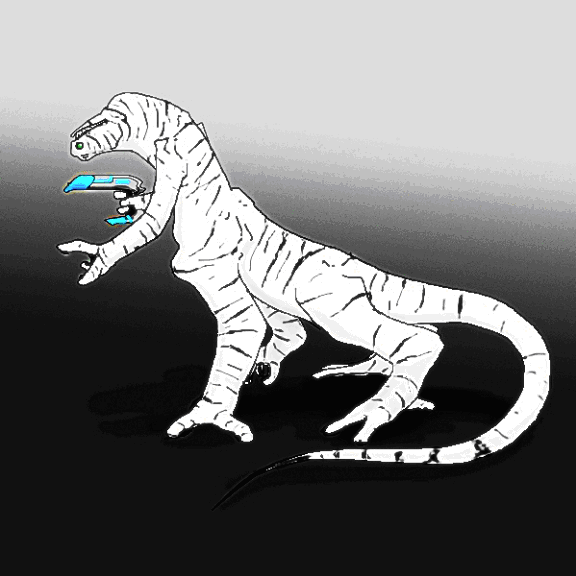
\includegraphics[width=\textwidth]{images/Aera.png}
}
    \caption{Aeran. Head is non-canonical and should treated as such. Rest of body is a reasonably solid depiction.}
    \label{fig:Aera-body}
\end{center}
\end{figure}


\subsection{Habitat}
The Aera homeworld was, prior to changes imposed by the technological
advancement of the Aera, a nearly seasonless planet with an
oxygen-nitrogen-neon atmosphere, on whose surface were a single large
landmass and many large and small islands. The mainland was nearly
entirely covered with jungles and marshgroves, with only small belts
of more sparsely overgrown land on the northern and southern reaches
of the continent. The rich jungle land was home to all sort and manner
of parasites, predators, diseases, and competitors for food. It was in
this vast, dark jungle that the Aera arose into sentience, tool use,
and civilization.

\subsection{Culture}
Aera culture is highly organized and decidedly hierarchical, but in
the form of a meritocracy rather than an aristocracy. While what has
constituted merit has morphed over the millennia since the first Aera
tribes selected work crews to cut back the encroachments of the jungle
upon their early settlements, given the relative position of the
pre-technological Aera in their local food chain, there has long been
a favoring of cleverness and determination over raw strength. The
current social and vocational position of any Aera is immediately
indicated by the color and pattern of an individual's coverall. The
Aera are ruled by a subset of the highest caste, with membership in
the oligarchy changing whenever either an individual steps down, or a
third of the other members call for a member's replacement. New
members must be confirmed by two thirds of the current oligarchy. It
is much more common for members to voluntarily remove themselves from
power, believing themselves more useful elsewhere in society, than to
be cast out. An average stay in the oligarchy lasts a few Aera years.

The long struggle of the Aera against the erosion of their society at
the hands of the natural world has instilled in them a deep respect
for that which has enabled them to conquer their environment:
technology. Not only is the advancement of technology greeted without
fear, the social position of the artificer and the engineer is one
more greatly elevated than that seen in any pre-Diaspora human
society. What is feared is the unmastered and uncontrolled. Even after
the last war between Aera and Aera was fought, bringing the last of
the major islands under the control of the mainland, the Aera only
slightly relaxed their military investment. Perhaps in large part due
to their short lifespan, and the consequential rapid dying off of
adherents to old theories, science advanced quickly, and with the
understanding of their place in the universe came a belief that just
as they had been forced to fight back against the jungle to keep
themselves alive, so would they likely have to push back against all
that waited for them beyond their world. Thus, eight centuries ago the
Aera burst forth from their homeworld, not afraid, but determined that
nothing would stand between them and their indefinite existence.

{\bf Factions and Organizational Groups}
Listed below are noteworthy Aeran sub-factions and organizational groups: 
\begin{itemize}
\item Aeran Merchant Marine
\end{itemize}

\subsection{Religion}
The nature of the Aera homeworld never inspired much belief in any
sort of loving deity. What began as a collection of local deities
coalesced, through conquest by what was to be the dominant group on
the entire planet, into a single pair of entites, one force of
creation, and one of destruction, both abstract, and both uncaring. As
time progressed, and the Aera advanced, these entities progressively
lost entity status and drifted into the realm of spiritual
concepts. Becoming more self-centered in their exploration of
existence, destruction morphed into personal death, and creation into
species survival. Organized religious activity among the Aera, such as
it was, ceased centuries ago, but the impact on their culture of the
concepts of death and survival is still quite strong. Indeed, Aeran
mausoleums are said to be, quite possibly, the only pieces of Aeran
art that might ever be considered beautiful. The Aera respect death,
but value is placed on the accomplishments made in the face of one's
imminent demise. All Aera are cremated, and the repositories for such
remains are vast public works, filled with displays of the
accomplishments of those entombed within, those who contributed
greatly to the species being rewarded with physical space devoted to
listing their deeds, and the rest consigned to a rotating schedule of
intermittent holograms and access via terminal displays. It is in such
places that an Aera would go to ponder, in silence and solitude,
relenting briefly from the near tireless schedule of a short-lived
species, the nature of its existence.

\subsection{Miscellaneous}
The Aera use a redundant numbering scheme:
Radix 3, digits drawn from the set of values {-2,-1,0,1,2} 

\section{Ancients}

\subsection{Physical characteristics}
There are precious few preserved remains of either species A or B
(especially B), so knowledge of their physiology is pieced together
from various, sometimes conflicting sources.

{\bf Species A}

Species A were moderately sized beings, between 1 - 3 meters in height, and no more than 2 meters in diameter. 

{\bf Species B}

Species B were smaller beings, no more than a meter wide, high, or thick. 


\subsection{Habitat}
The native habitats of these creatures are unknown. Given the nature
of the planets they settled, it can be assumed that they were
carbon-based lifeforms, and that at least of one of the two was an
oxygen breather.

\subsection{Culture}
Beyond their technological advancement, little is known. 

Excerpt from "A Brief History in Time and Space" 

"While there is much contention about the nature of the predecessors
of the Ancients, the Ancients themselves left enough rubble strewn
around the galactic arm to convince even a fairly hardened skeptic of
their having dwelled in these parts. The Ancients appear to have been
made up of at least two major species groups, and interacted with at
least three others, albeit it is not known whether these were client
species, or contemporaries from another part of the galaxy. Their
reign over this region lasted until about 1 to 2 million years ago,
whereupon they rapidly ceased to be present. There is a wealth of
evidence that severe infighting played some part in the destruction of
the Ancients, but, assuming there were victors in such a conflict,
little is known of what became of them.

The best source of such evidence, however limited, is the Uln
homeworld. While they are quite sensitive about the subject, the
widely held belief among the major races is that the Uln are the
descendants of the Ancient's equivalents of lab monkeys. The Uln
culture sprang up among the remains of a sprawling set of Ancient
structures... if they hadn't been so ill prepared for the gifts they
unintentionally received, they would have conquered the entire
arm. Fortunately for the aspirations of dominance held by other
species, the Uln were decidedly unprepared. Indeed, they spent so much
time blowing each other up with weapons they didn't entirely control
that it is a wonder that either they or the ruins on their planet
still survive.  The ruins, however, did not escape unscathed from the
genesis of the Uln culture. While assuredly the largest known source
of information on the Ancients, the ruins deliver little coherent
information about many key aspects of the Ancients' existences,
largely due to vast portions of many buildings having been turned to
dust."

To clarify, the statement about the Uln possibly having been able to
conquer the arm is contingent upon them NOT having blown most of the
ruins up, along with the devices they were using to blow each other
up, and large portions of their own species. No superweapons as such
are known to be currently possessed by the Uln. The Uln are in
possession of one particularly impressive piece of Ancient technology
(what is known as the Sul-Gatwa high castle), but it's potential is
effectively limited to the defense of their homeworld. However, even
as heavily damaged as the finds on the Uln world are, they remain the
best source for archeological research, and research visas remain a
large part of the Uln economy.

Why would this blasted planet be the best source of artifacts?
Because, unlike most of the planets that seem to have been inhabited
by the Ancients, it didn't have it's entire surface slagged, get
broken into a debris field of billions of pieces of rock, or become
pockmarked by craters implying assault equivalent to prolonged
planetary bombardment by 500Km wide asteroids.

Despite this, the occaisional piece of debris is found in such
places. However, the only officially reported finds of
fully-functioning Ancient technology have been the nano-plague and
various minor finds on the Uln homeworld.

The largest known piece of Ancient technology is the Sul-Gatwa high
castle. Whether or not it is technically functional is a matter of
some scholarly contention - the object is a slagged chunk of some
small moon sized ship or station. No systems appear to be remotely
functioning. However, what information has been declassified by the
Uln Royal Ingatwa fleet and confirmed via espionage implies that the
structure is so dense that it should have collapsed under its own
gravity into a solid mass - however, as the material that the high
castle is composed of defies the best efforts of science to explain or
duplicate (it has been jokingly dubbed "unobtainium") it could just be
some intrinsic property of the material and not evidence of
functioning gravitics. While the high castle has none of it's original
equipment and is, in essence a giant chuck of debris in orbit around
the Uln homeworld, every indication is that it retains the potential
to absorb absurd amounts of damage, and, as such, the centuries that
the Uln have spent arming it with their own weapons have made it the
most formidable planetary defense station known to exist. Its
existence, the threat of the Uln destroying what remains of the
Ancient artifacts, and general opinion that any of the major powers
could pen the Uln into their home system if necessary are believed to
be the primary factors responsible for the Uln remaining independant
entities.

Small fragments of Ancient technology, even completely non-functional,
fetch a fair price at any research facility or university
planet. Functional pieces of Ancient technology, even if relatively
useless, are of exceptional value, and it is not unheard of for
persons to attempt to make a career out of artifact prospecting,
subsisting on the rewards from finding small pieces of debris while
waiting for the big catch of working Ancient tech. However, as time
progresses, the easier pickings have already been scavenged, and
exploration of progressively more hostile environments has become
necessary to sustain the trickle of finds.

\section{Bzbr}

The Bzbr are a psuedo-reptilian species found on a jungle planet by
the Aera early in their expansion. The discovery of organized alien
intelligent life, even if harmless in it's neolithic state, furthered
Aera convictions about the dangers of the universe, even as they
worked to co-opt the Bzbr.

\subsection{Physical characteristics}
A Bzbr most closely resembles a jungle-green, copper-highlighted
1.5-meter long, ten-legged, arboreal reptilian with a nearly meter
long prehensile tail. Each limb has four segments, the fourth being
the hand/foot equivalent. The rear six legs are built for jumping, and
are used only for locomotion, the two underslung short arms primarily
for food manipulation, and the two forward inline limbs primarily for
gripping branches or other such objects, arching upwards and forward
from the rest of the body, in contrast to the other inline limbs,
which proceed upward and outward from the torso. Lacking vocal cords,
the Bzbr communicate in a simple language consisting of varied buzzing
tones produced by rubbing their feeder limbs together and motions of
the gripping limbs.

The Bzbr have three genders, breeder, broodherd, and
gatherer. Gatherers are the most common gender, and conduct all
hunting activities. Breeders are smaller than the gatherers, and
forage close to the nest area for roots and nest building material. In
far smaller number than the breeders or gatherers are the broodherds,
larger, stronger, sterile, and existing solely to protect the young
and territory of their sisters. Normal Bzbr nest groupings number in
the few dozens of adults. Bzbr are exceptionally short lived, living
only 35 - 40 years, even with modern medical technologies, but, given
their small size, this is not entirely unexpected.

\subsection{Habitat}
A world of jungle islands, spontaneous firestorms due to the high
oxygen content of the atmosphere, and extreme seasonal weather shifts,
the Bzbr homeworld can be safely considered unpleasant to all of the
known spacefaring races.

\subsection{Culture}
Adopted by the Aera out of some combination of pity and sympathy for
similar jungle origins, the Bzbr were pulled straight from the stone
age to the FTL age. Adapting about as well as can be expected to this
rapid change, many Bzbr simply went insane trying to adapt, but after
a few generations, the Bzbr had come to accept the new reality, even
if they were, due to rather much less than genius level average
intelligence, ill equipped to fully understand the full complexity of
it. Although not particularly bright or creative, the Bzbr are
actually quite good at both remembering and following instructions,
and have come to be used in various Aera space construction projects,
where they are valued for their ability to deftly maneuver in small
spaces and to leap from girder to girder. Bzbr, are, however, never
seen far from their Aera Patrons, as they are quite lost without
them. The Bzbr still, to some great degree, see the Aera as messengers
of the gods, having delivered them from the horrors of their world,
even if they know the Aera to be both mortal and fallible.

\subsection{Religion}
Though the Aera have attempted to convince them to do otherwise, the
Bzbr engage in hero-worship of the Aera. A majority of the Bzbr are
convinced that the actions taken in this universe play out in other
planes where the great nest of all life is threatened by chaos. They
believe that the Aera, by having brought greater order to their lives,
make them all great warriors in the other planes.

\subsection{Miscellaneous}
Bzbr use Aeran numbers. 

\section{Dgn}

The Dgn, like their brethren the Shmrn, are the descendants of a joint
Shaper and Lightbearer uplifting program begun with dextrous, tool
using, but pre-civilized saltwater marsh dwellers. The Dgn are the
branch cultivated by the Shapers and remain an integrated servant
class in Shaper society.

\subsection{Physical characteristics}
See images ~\ref{fig:Dgn-body} for bodyplan and ~\ref{fig:Dgn-motion} for locomotion (the Avian style is closest): 

\begin{figure}
\begin{center}
\makebox[\textwidth][c]{
    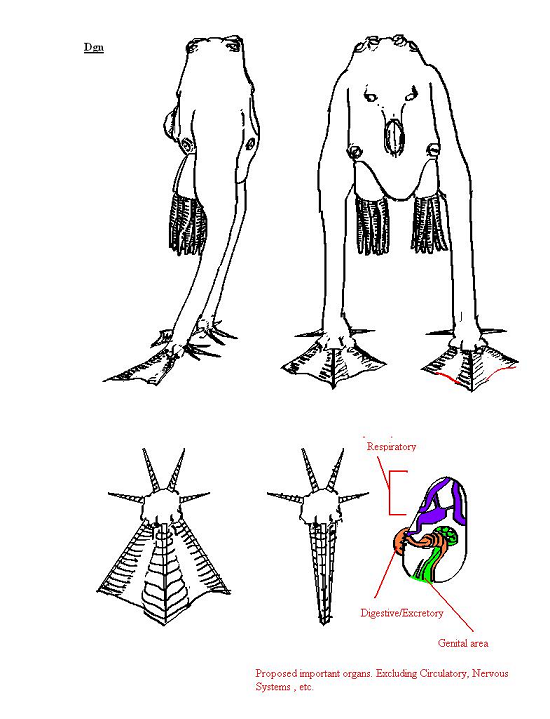
\includegraphics[width=\textwidth]{images/Dgn-body.png}
}
    \caption{Dgn body-plan}
    \label{fig:Dgn-body}
\end{center}
\end{figure}

\begin{figure}
\begin{center}
\makebox[\textwidth][c]{
    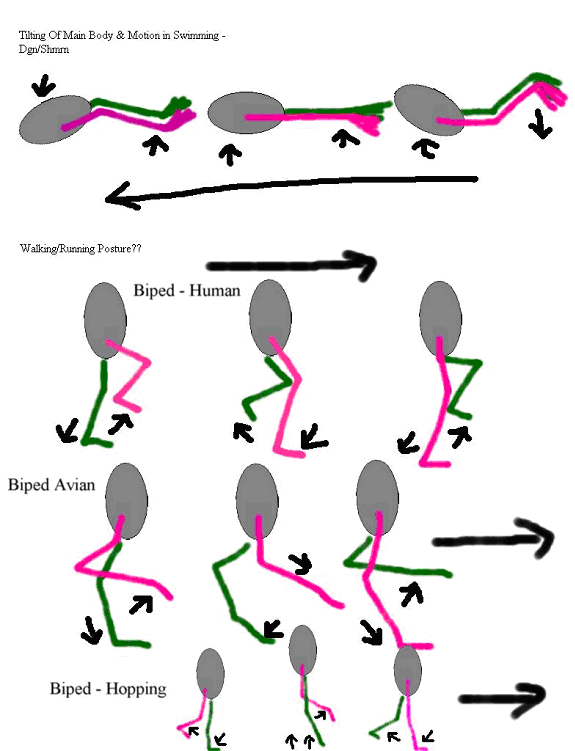
\includegraphics[width=\textwidth]{images/Dgn-motion.png}
}
    \caption{Dgn locomotion on land and in water}
    \label{fig:Dgn-motion}
\end{center}
\end{figure}



See Also: Shmrn (~\ref{subsec:Shmrn-species})

Through genetic engineering their life expectancy has been extended to over 50 years. 

\subsection{Habitat}

The Dgn can breathe in both atmospheric and aquatic conditions,
provided that there is sufficient oxygen dissolved in the water. They
do, however, require either a humid land environment, or frequent
re-wetting to keep both their skin and breathing orifices from drying
out. The native Dgn habitat ranged from coastal saltwater marsh-land
to tidal flats and into the coastal shallows themselves.

\subsection{Culture}

What native culture existed among the pre-modified Dgn has been
greatly altered. Bred for servitude, the Dgn are not greatly renowned
for intellectual achievements. The Dgn exist as a servant race for the
Shapers, working on nearly all Shaper aquatic projects, and filling
other unwanted roles in society. The one noted exception to this rule
is the use of Dgn as medical assistants in Shaper hospitals, where
their dexterity has proved them faster than humans at prepping the
injured for surgery. While the rights of the Dgn are well defined by
the Shapers, and abuse is not at all tolerated, their rights are not
the same as those of the Shapers, and if the Dgn are to be considered
citizens of the Shaper political body, then they are, at best, second
class citizens. The Shapers have built them to not be overly concerned
about this (the Shapers having had a different vision of what they
desired from their uplift than the Lightbearers, who were more
concerned with continued evidencing of their believed and beloved
superiority over lesser species). One cannot say that the Dgn are
entirely pleased with their position, but neither can one say that
there is fertile ground for revolt, as the Dgn do not seem to possess
within them a particular desire to be forced to decide their own
destinies. As the Dgn do not complain and the Shapers do not overtly
or actively seek to mistreat the Dgn, their freedom is something
sought after by activist groups rather than brought about by an armed
foreign entity.

\subsection{Religion}

Whatever glimmerings of disorganized religous beliefs they may have
had as more simple creatures have been lost. Currently prohibited from
engaging in organized religious activities due to historic fostering
of undesired solidarity.

\subsection{Miscellaneous}
Dgn use Human numbers. 

\section{Hoffman's blobs}

Hoffman's blobs are seemingly non-sentient creatures living in the
void of space. They were discovered by Burno Hoffman in the Barnard's
Star system.

\subsection{Physical characteristics}
Very little is known of those bizzare interstellar beings. The last
sighting has been in the Galileo system. Scientists are now flocking
to study these creatures before they leave, attempting to determine
how it is that they are able to sustain themselves in the void of
space. Observations suggest their size varying greatly, with the
largest individuals proving as large as a space cruiser, and the
smallest only the size of a shuttlecraft. It is uncleaer whether these
differences are attributable to age or polymorphism. The creatures
appear to primarily be drifters, but are capable of some acceleration.

\subsection{Habitat}
Hoffman's blobs live in the void of space. Since they were discovered
there have been six sightings of them, most recently in the Galileo
system.

\subsection{Culture}
There has not been any exhaustive research on the behavior of
Hoffman's blobs yet. From previous observations, it appears they
travel in flocks of about a dozen units.

\section{Humanity}

Table~\ref{table:relevantspecies} shows the relevant species in the UTCS time period and notes their organizational relations. FIXME (placeholder)

\begin{itemize}
\item	Homo Sapiens Sapiens (Faction with highest population percentage: Purists) 
\item	Homo Sapiens Superioris (Faction with highest population percentage: Shapers) 
\item	Homo Sapiens Cyberis (Faction with highest population percentage: Mechanists) 
\item	Homo Sapiens Pluralis (Faction with highest population percentage: Andolians) 
\item	Homo Sapiens Suprahomo (defunct) 
\item	Homo Sapiens Cosmonatalis (Faction with highest population percentage: Spaceborn) 
\end{itemize}
\subsection{Physical characteristics}
\begin{itemize}
\item Homo Sapiens Sapiens
\index{Homo Sapiens!Species info}
\index{Homo Sapiens!Homo Sapiens Sapiens}

Although small changes have occurred over the millenia, a great
percentage of the human population remains without intentional genetic
or physical modification, and thus remains not too far removed from
the humans of more ancient history. Whether through simple lack of
resources, lack of desire, or rejection of change, Homo Sapiens
Sapiens, unmodified except for the genetic drifts incurred over
centuries of colonization, remains the most populous of the human
subspecies.

\item Homo Sapiens Superioris
\index{Shaper!Species info}
\index{Homo Sapiens!Homo Sapiens Superioris|see {Shaper}}

Many eugenics programs have been launched in human history, but none
have been so successful. The path of self-affected evolution via
active genetic redesign has lead to a strain of humanity stronger,
more durable, more resistant to disease and injury, of higher average
intelligence, enjoying longer life-spans, and possessing keener
senses.  Assuming that the universally ink-black UV-resistant skin and
complete lack of any hair other than the signature blue-white
eye-brows is not disconcerting, any Superioris is almost certain to be
considered physically beautiful, but it takes some experience to
discern one Superioris from another. However, these benefits come at
the cost of much higher sustanence requirements, and a tremendous
narrowing of diversity.

\item Homo Sapiens Cyberis
\index{Mechanist!Species info}
\index{Homo Sapiens!Homo Sapiens Cyberis|see {Mechanist}}

Having replaced many of their body parts with mechanical equivalents,
or having forgone any pretense of human form, these cyborgs cover a
diverse and vibrant set of body types. Those with total body
replacement can usually pass anything short of close inspection if
they're willing to deal with maintenance of a synthetic flesh
exterior. If the goal is, as is often the case, to adapt the body to
the demands of work or habitat, anything from mining attachments to
full strength-enhancing endoskeletons could be an integral part of the
form. Locomotion seen to date ranges from bipedal to poly-pedal,
tracked, wheeled, or even sets of thrusters. In addition, this sort of
technical enhancement may provide the ability to extend one's lifespan
indefinitely if the base neurological systems have already been
altered to be non-senescent (provided one has access to regular
maintenance service). However, no matter how modified they may be, at
the least, portions of their brains and nervous systems remain.  While
communities of such modified humans exist on the worlds of many
factions, the Mechanist faction is the only full-fledged meme-group
centered upon the post-flesh goals of Homo Sapiens Cyberis.

\item Homo Sapiens Pluralis
\index{Andolian!Species info}
\index{Homo Sapiens!Homo Sapiens Pluralis|see{Andolian}}

While various communities have arisen that rely upon linked
existences, none save the Andolians have sufficiently differentiated
themselves en masse from the rest of humanity to be a discernable
grouping. Implanted at birth with hardware that allows data-net access
and an array of almost constantly transmitting sensors, a permanently
linked existence has rendered this strain of humanity notably
different in culture and mentality from all other strains.  While
every Pluralis retains its individuality, each is awash in a similarly
accessible sea of information. Culling from the group of those not
capable of entering into such an existence combined with a willingness
to engage in limited crafting of offspring has also lead to small but
noticeable genetic drift over the past 800 years. Implantation is
universal, and the use of synthetic or mechanically enhanced body
modifications is not uncommon, but the desire for total body
replacement present in the Cyberis strain is absent.  The linked
existence and general cultural proclivities of the Andolians have
brought them to near unity on their religious doctrine. While an
Andolian would refer to his/herself as a devout skeptic existing in
the absence of proof of the metaphysical, many others find it simpler
to call them Atheists.  While not overly concerned with improving the
physical form, health-related genetic traits deemed undesireable have
been recorded and then excised from the gene pool. When isolated for
long periods of time from any data-net, Pluralis individuals often
experience pronounced withdrawal symptoms, earning them the nickname
"Link-Junkies".

\item Homo Sapiens Suprahomo (Lightbearers) (Nearly Extinct) 
\index{Lightbearers!Species info}
\index{Homo Sapiens!Homo Sapiens Suprahomo|see {Lightbearers}}

One of the earlier factions to aggressively expand outward in the FTL
era were the Lightbearers, a meme-group built around the development
of a supra-human race. Believing the human form to be the sacred
forefront of evolution in the entire galaxy, they sought to claim the
place of their distilled and purified strain at the throne of all
sentients.

\item Homo Sapiens Cosmonatalis
\index{Spaceborn!Species info}
\index{Homo Sapiens!Homo Sapiens Cosmonatalis|see{Spaceborn}}

Crafted as a slave race by the now defunct Light-Bearer faction, the
Spaceborn, as they are commonly referred, remain frail and
over-specialized, incapable of surviving in planetary
environments. Instead, as they were designed, they spend their entire
lives in micro-gravity. The Spaceborn have a unique cardiovascular
system superbly tuned to life outside of a gravity well.  Their bone
structure, however, is a less cheery affair, and the Spaceborn, though
not suffering the degenerative effects of planetborn entities in
prolonged micro-gravity, never had much durability in the first place
and are weaker and more easily injured. They are almost universally
tall, lanky, and flexible, and all are possessed of a rather pallid
complexion tending toward a slight reddishness. Spaceborn frequently
begin developing severe medical problems between the age of 60-80
Earth years, giving them a somewhat shorter life expectancy than that
of the other subspecies.  Almost all Spaceborn live in habitats
situated in Andolian Protectorate space, having relocated from
Light-Bearer space after liberation from that faction.
\end{itemize}

\subsection{Habitat}

Originating on the third world of the Sol system, all variants of
humanity, even Homo Sapiens Cyberis, are most comfortable in
Oxygen-Nitrogen atmospheres, and temperatures not overly distant from
294 Kelvin.

\subsection{Culture}
Listed below are links to noteworthy human Meme-groups, organizations,
and governments:

FIXME 

\subsection{Religion}
Among the most mixed and varied in the known galaxy, running the gamut
from atheists to zealots. Refer to the individual groups for more
information.

\subsection{Miscellaneous}
Base 10. 

\section{Klk'k}
FIXME 

 
One of only five extant species to have achieved some measure of
space-flight prior to contact with other sentients, the Klk'k had what
can be readily argued as the worst first-contact experience on
record. Although the Andolian backed Ktah Restoration Project did much
to stem and repair the damage caused by the Lightbearers during their
occupation of Ktah, nearly a quarter of the Klk'k species were killed
by the Lightbearers, the majority of the deaths stemming from the
Lightbearers retargetting their fusion-tipped anti-orbital defense
missiles for ground impact and launching all batteries in a
scorched-earth response to the Hoshino Uprising. While the
laser-induced fusion warheads were exceptionally clean in the
radiologic sense, the scale of the bombardment was such that there
remain a number of areas of Ktah which have not fully recovered, even
at more than two centuries remove.

Currently, almost all Klk'k are citizens of the Andolian
Protectorate. While the Klk'k are self-governing over their own
colonies on domestic matters, with a government centered in Ktah, they
defer to the Andolians on external affairs. A significant minority of
the Klk'k population have become active adherents to the Andolian
meme-group, living integrated existences networked into surrounding
Andolian populations. Several mixed-species colonies featuring both
Humans and Klk'k exist, and there is both a human and Klk'k presence
on all Purth worlds.


\subsection{Physical characteristics}
average height range 4.5 to 5.5 feet (in meters?)

long, largish feet, reverse jointed knees, large easily splayed hips,
excellent jumpers, thick, disproportionally long, muscular legs in
proportion to generally much skinnier tops

wide, short, fair lengthed, back-bottom flanging head, with back
facing nostrils at the rear base between neck and jawbone

jaw is wider than head on each side. because of angle, more teeth on
bottom jaw than on top, bottom jaw teeth face slightly in, top jaw
teeth face slightly out

mouth contains 2 tongues. has no connection to air passageway. has
resonant "click" cavity in front top of mouth, behind and below the
rear of the bone ridges forming the eye sockets

eyes are large and wide set, and the sockets prononouced in their
bonyness

ears, such as they are, are 2 long curved ovoids, extending forward
from just behind and below the top of the jaw joint to somewhat even
with the top of the jaw joint and in front of the joint.  Mostly flush
with the skull, each ear is a series of cartilige-analog ridges
protruding slightly out from the side of the head to focus sound into
a central shallow curved trough, the bottom of which has numerous tiny
folds of hair-lined skin atop a drum

See additional discussion (later in document)

Figures ~\ref{fig:Klk'k-body-front},~\ref{fig:Klk'k-body-side}, and~\ref{fig:Klk'k-body-head} are poorly drawn sketches of the basic Klk'k body plan. Though
they show the general outlines, they are inconsistent as to whether
they are showing skeletal/muscular/etc. structures and details (to be
taken as rough guidance only - not canonical due to poor
implementation of desired visible outcomes (i.e. jacks can't draw
worth a damn))

\begin{figure}
\begin{center}
\makebox[\textwidth][c]{
    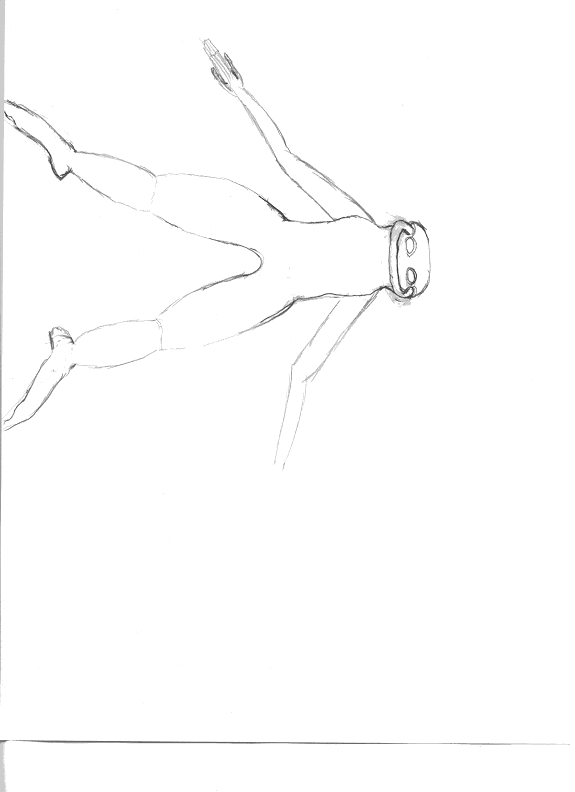
\includegraphics[width=0.75\textwidth]{images/Klk'k-bodyplan-front.png}
}
    \caption{Basic Klk'k body plan (front)}
    \label{fig:Klk'k-body-front}
\end{center}
\end{figure}
\begin{figure}
\begin{center}
\makebox[\textwidth][c]{
    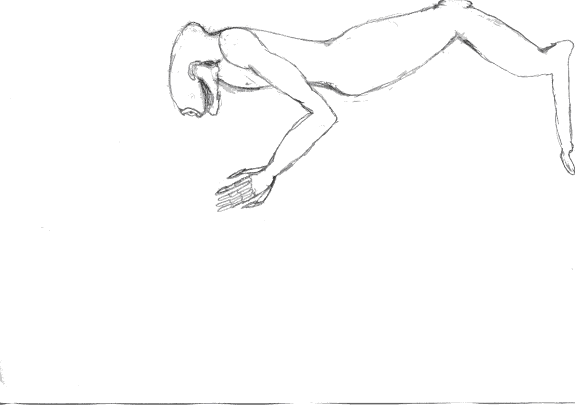
\includegraphics[width=\textwidth]{images/Klk'k-bodyplan-side.png}
}
    \caption{Basic Klk'k body plan (side)}
    \label{fig:Klk'k-body-side}
\end{center}
\end{figure}
\begin{figure}
\begin{center}
\makebox[\textwidth][c]{
    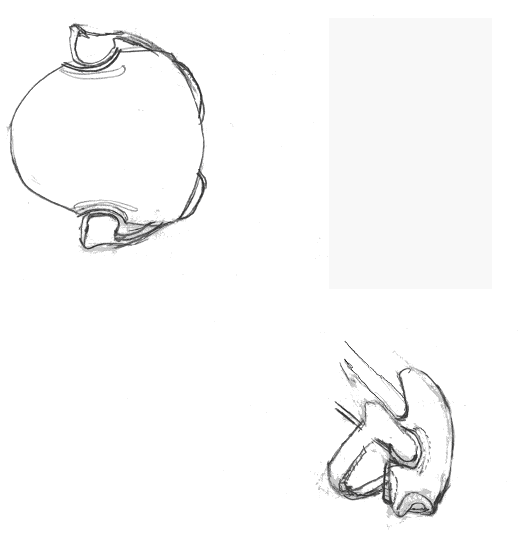
\includegraphics[width=\textwidth]{images/Klk'k-bodyplan-head.png}
}
    \caption{Basic skeletal structure of Klk'k head}
    \label{fig:Klk'k-body-head}
\end{center}
\end{figure}

The most anthropoid of the sentient species that humanity has
encountered (admittedly, two arms, two legs, two eyes, one head is
enough to place them ahead of most others), the Klk'k are nonetheless
notably alien in nature. Bipedal, with bilateral symmetry, the Klk'k
stand 1.3 to 1.5 meters tall on two splayed, reverse-jointed, muscular
legs, balancing on extremely elongated feet. Two arms,
disproportionately long by human standards, drape down from the
shoulders, each ending in a hand with four wiry fingers and two
thumbs, one on each side. The thumbs have something resembling nails,
while the rest of the fingers terminate with a hard, leathery, callus
covering the top and front, the finger-tips remaining fleshier. Klk'k
toes terminate in short, thick, blunt, stubby claws far more useful
for climbing than for tearing. The Klk'k head is wide and somewhat
squat in comparison to its breadth, being noticeably wider, at the
bottom, than the Klk'k neck. The Klk'k face features two large eyes
and a mouth that opens most of the way back to the jaw hinge. The
jawbone continues in an outward direction somewhat as it goes down
from the skull, further accentuating the width of the Klk'k head. The
Klk'k air passageways and digestive tract are separated. Breathing is
performed through two rear-facing nasal openings, one on each side of
the back of the head, situated behind and under the jawbone
attachment, opening where the head curves back to meet the neck. The
two eye sockets are protected by pronounced brow ridges. Inside the
mouth is a resonating click cavity, and two tongues. Klk'k have
several smaller, sharp, front teeth, and a smaller number of larger
grinding teeth, present only at the back of the mouth. Klk'k ears have
minimal external presence compared to human ears, presenting
themselves primarily as a furrow curving back and down along each side
of the Klk'k skull. The ears are water-tight, and Klk'k underwater
hearing is significantly superior to that of humans.

Klk'k are hairless, and the skin tends toward a swampy, uneven
green-brown, excepting the secondary sexual characteristics which
express themselves as thin, rosy-to-purplish highlights on the sides
of the head, hips, wrists, and ankles. Skin tends to be smooth, and
slightly leathery in texture, but a substantial layer of subcutaneous
fat keeps it from being hard to the touch. Both sexual and excretory
organs are positioned similarly to those of humans, at the posterior
of the torso. The Klk'k have two genders, the female of the species
tending to be the larger of the two, and distinguishable, among the
adult population, by the presence of more purple, rather than rosy,
highlights. Distinguishing between the genders of Klk'k children is a
more difficult task for the untrained human eye.

Klk'k have single fetus (with few exceptions) internal pregnancies,
and exceptionally long gestation periods. The later stages of the
pregnancy are extremely debilitating to the mother, eventually leaving
her nearly immobile as the fetus grows to increasing size and the
birthing blister migrates progressively closer to the
surface. However, at birth, the newborn Klk'k can already walk, swim,
and consume normal food.

Klk'k speech is produced primarily as a combination of vowels and
tones from the nasal airways and clicks from the tongues and
resonating chamber. Manipulation of the closures to the nasal airways
also produce a smaller number of consonants. The tonal nature of each
airway is independent, and harmonics have semantic and syntactic
meanings in most of the native Klk'k languages. The iconic Klk'k nasal
horn takes explicit advantage of the dual-tonal capabilities of the
Klk'k. Some human observers have likened Klk'k speech to listening to
a pair of Hawaiians having an animated conversation with a pair of
Khoisan, but most real xeno-linguists attempt to discourage such
simplistic comparisons as more misleading than informative. "Klk'k" is
itself an anthropic transliteration of their word for themselves,
likewise for Ktah, and Tk'latl, etc. As the Klk'k have proven far more
adept at understanding spoken human tongues, than the reverse, even if
they cannot produce the full range of human sounds, the anthropic
forms have become accepted standards, rather than requiring all humans
to utilize translator devices to refer to anything of Klk'k
origin. Klk'k living or traveling among humans tend to equip
themselves with vocalizing augmentation devices that fill in the
missing gaps in their ability to emulate human speech.

\subsection{Habitat}
Ktah is a warm, wet world with an Oxygen-Nitrogen atmosphere and vast
open stretches of ocean surrounding the two major continental
bodies. The Klk'k originated on the smaller of the two continents,
developing amidst the seemingly endless criss-cross of rivers and
bayous that dominate it. Though not amphibious, the Klk'k are quite at
home in the water, being excellent swimmers.

\subsection{Culture}
Humor plays a deep and intrinsic role in Klk'k culture, far beyond
that in any human one. While the Klk'k equivalents of humor and even
laughter have strong similarities to their human counterparts, the
situational appropriateness of humor is viewed quite
differently. There are few things that necessitate a somber decorum
for a Klk'k - they would see nothing inappropriate about joking and
laughing at someone's deathbed, funeral, execution, summit, board
meeting, intelligence briefing, etc. Indeed, quite the opposite is
true. Even war and combat are not seen as entirely serious realms --
there are numerous Klk'k stories involving tales of foes refraining
from death blows because each was waiting for the punchline of the
other's joke. Humor is also seen as appropriate in public actions,
officials, and governmental entities. In one particularly long-running
tradition, legislation is frequently put forward to change the Klk'k
anthem for the duration of a visiting dignitaries arrival in order to
make atrocious puns.

Being unable to find or generate humor in one's situation is a sign,
in a Klk'k, of a present or imminent psychosis, if often only a
temporary one. Klk'k can be riled to an indignant rage that, if short
lived, is still disturbing in its intensity. In Klk'k martial arts,
such as Amakakt, sparring contestants are often required to keep a
running dialog of humorous insults. If one of the combatants becomes
noticeably silent, the match is suspended, as it is a sign that
control has been lost, and the onset of rage may be approaching.

The basic Klk'k family unit is the the bond-set, based around a
mutually polyamorous clique arrangement. A bond-set usually consists
of 3-6 adult Klk'k and their assorted children, with the parentage of
the children coming from any arbitrary pairing within the
bond-set. Bond-sets consisting of only 2 Klk'k, save as a result of
the death of additional members, or as an initial state, are
considered strange, and their members potentially dysfunctional if
that arrangement persists. Bond-sets will continue to grow over time
by mutual interest in inclusion until they reach a steady point for
the individuals involved. Bond-sets with more than 6 members exist,
but are rare, as finding large numbers of co-interested partners is a
non-trivial task. Four members is the median expectation, and many
bond-sets of three partners will delay having children until a fourth
has joined. Some researchers believe the extended size of the basic
family unit to have roots stemming from the degree to which the later
stages of Klk'k pregnancies are completely incapacitating, leading to
a need for a larger supporting family unit.
\begin{itemize}
\item Bond-set Naming Conventions

The dominant culture for quite some time has used a strict two-name
scheme. When a bond-set is formed, the members choose a name for
themselves, and that is the bond-set name for those children raised by
that set. If the set changes, through addition, the name may be
changed or it may be kept, but the children will retain the old name,
unless very young. If the set changes through attrition, the name does
not change in order to honor what was, even if it is no more. One is
known by one's bond-set name (the name of those who raised you) and
your personal name, usually given in that order, thus Klk'k names are
not lineage tracing beyond a single generation.

\item Clothing and Ornamentation

Nudity was not a big deal in any notable pre-contact Klk'k culture,
and continues to be of little concern except among those Klk'k
visiting human worlds obsessed with particularly archaic
taboos. Common Klk'k coverings are as much practical and protective as
shielding from the public eye, featuring pockets, belts, places to put
or hang things, footwear, and isolated pieces to prevent scrapes and
scratches to various sensitive areas.

Klk'k style uni-gender semi-formalwear tends to be variants on a
loose, sleeveless (there is fabric straight from shoulder to neck, but
no collar), single-piece garment that runs completely flat across the
front, tapers slightly out from waist down and is slit in the back
somewhat below the end of the torso (the rear opening being convenient
for the Klk'k as their legs bend opposite those of
humans). Ornateness, except in extremely formal clothing, is highly
restrained, with patterns being limited to the edges and waist area,
running in thin seams around the garment. The prime regions of Ktah
are quite humid, and ostentatious layering would not have been
comfortable. Those looking for a more vibrant appearance tend to do so
with body paints on exposed skin rather than additional
clothing. Informal Klk'k clothing tends towards a short, loose skirt,
with tops, if any, varying by region.

There is also specific clothing to show respect, show allegiance, and
traditional body-paintings and tattoos. In particular, Amakakt tattoos
are expected among those practicing the martial art. A Tk'latl is
tattooed on the upper left topforearm/shoulder area, with annotations
denoting rank and record in Amakakt (the martial art heavily featuring
said Tk'latl). The ranking is above the Tk'latl, and consists of a
series of vertical bars of different color, denoting increasing ranks
attained, from left to right. A history of the matches is recorded in
colors corresponding to the rank of the opponents, and lies below the
Tk'latl, with vetical bars for victories and horizontal bars for
defeats.

Klk'k members of the Simons are known to frequently sport dynamic
tattoos, making their membership explicit when desired and hidden when
inconvenient.
\end{itemize}
\subsection{Religion}
The Klk'k frowned intensely upon organized religion even before they
settled under the wing of the Andolians. Klk'k history had been rife
enough with false prophecies and self serving church-like
establishments (including a theocracy that once dominated much of
Ktah) that the Klk'k analog to the Enlightenment had been rather total
in its sweeping reforms. Klk'k culture, however, has a long history of
veneration of ancestors, which continues in various ritualized forms
of behavior. There is no belief among the Klk'k that the deceased may
be contacted, nor is there any particular spiritual nature to the
reverence for those who came before, merely the conviction that it is
one's duty to honor the fact that, without them, one would not be.

\subsection{Miscellaneous}
Base 12, with numeral set derived from 2x2 entries in (2,3) double
base number system.

\section{Lmpl}

\subsection{Physical characteristics}
See Figure~\ref{fig:Lmpl} for image of a
Lmpl. Figure~\ref{fig:Lmpl-working} shows a Lmpl performing various
tasks.

\begin{figure}
\begin{center}
\makebox[\textwidth][c]{
    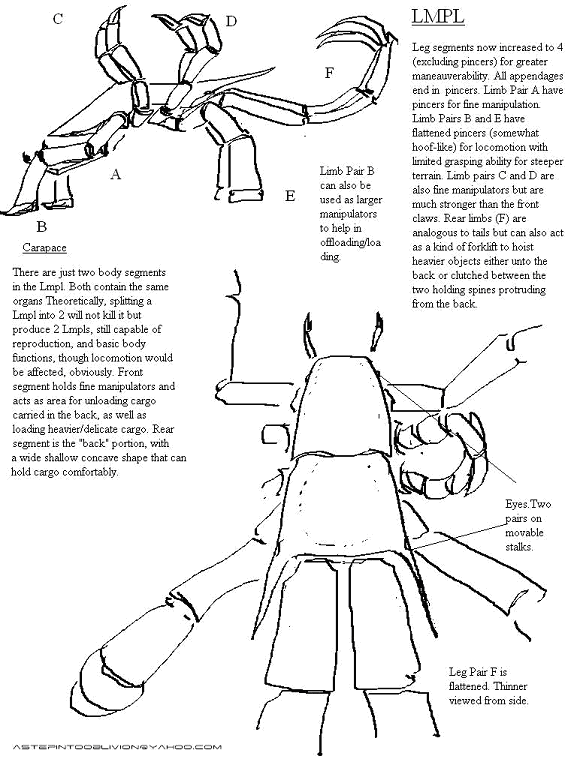
\includegraphics[width=0.75\textwidth]{images/Lmpl.png}
}
    \caption{Image of a Lmpl}
    \label{fig:Lmpl}
\end{center}
\end{figure}
\begin{figure}
\begin{center}
\makebox[\textwidth][c]{
    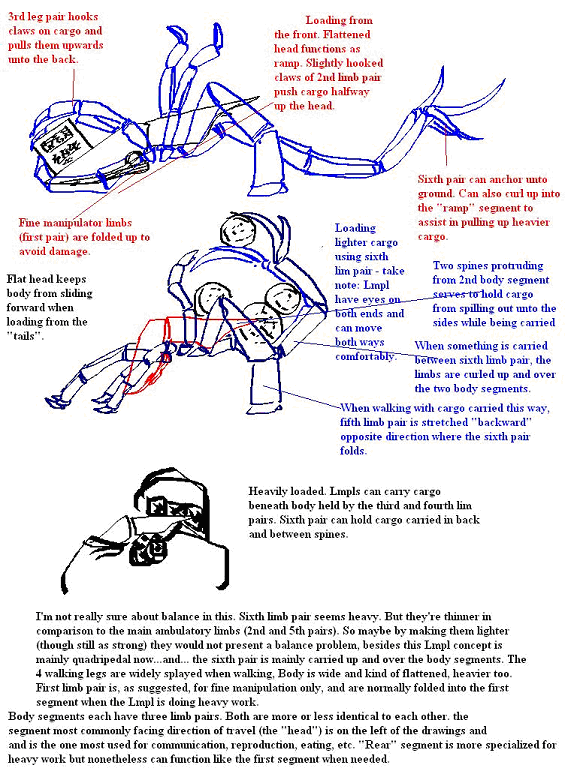
\includegraphics[width=0.75\textwidth]{images/Lmpl-working.png}
}
    \caption{Lmpl doing work}
    \label{fig:Lmpl-working}
\end{center}
\end{figure}


\subsection{Habitat}
Oxygen-Nitrogen 

\subsection{Culture}
Like the Nuhln, the Lmpl were a sub-sentient species that the Rlaan
selected for uplifting. The Lmpl were a project in adapting a lifeform
to an envioronment inhospitable to Rlaan workers. The Lmpl are
intelligent, but remarkably, and sometimes to a fault, single-minded,
though such is in keeping with their technical workforce mission. The
second of the two major uplift projects, the Lmpl are considered a
solid success, and enjoy their own niche role in Rlaan
society. Admittedly, as they are Oxygen-Nitrogen breathers, they spend
very little time actually in Rlaan society proper.

\subsection{Religion}
All Lmpl are adherents of Rlaanbzztkrlbzeentkaan (see ~\ref{Rlaanbzztkrlbzeentkaan}). 

\subsection{Miscellaneous}
The Lmpl use Rlaan numbers. 

\section{Mishtali}

The Mishtali were the first intelligent life forms Humanity came in
contact with, and at the time were enjoying a prolonged and happy
bronze age. Perhaps fortunately for them, the Unadorned were the
discovering faction, governing the Mishtali with a benign neglect. The
Mishtali managed the jump from a nomadic existence to being spaceport
baggage handlers quite well, all things considered, only eating a
fairly small number of colonists and tourists in the process.

\subsection{Physical characteristics}
See Figures~\ref{fig:Mishtali} and ~\ref{fig:Mishtali1} for details.

\begin{figure}
\begin{center}
\makebox[\textwidth][c]{
    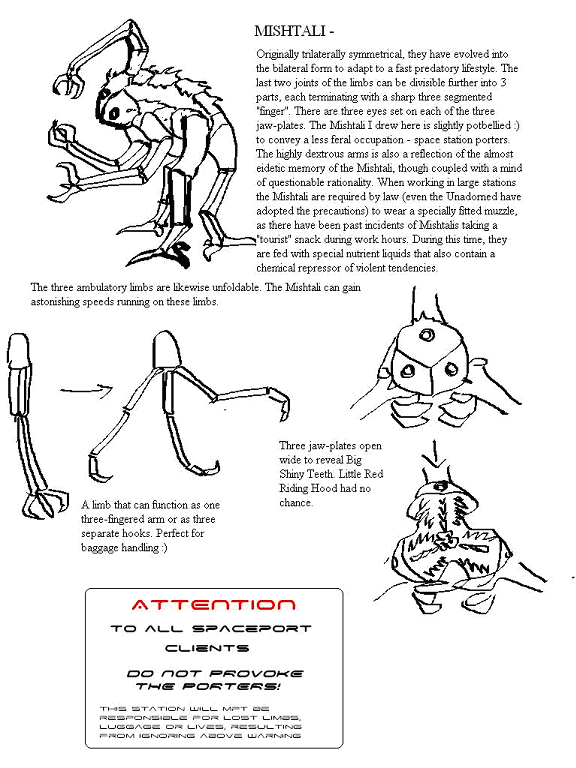
\includegraphics[width=0.75\textwidth]{images/Mishtali.png}
}
    \caption{Mishtali}
    \label{fig:Mishtali}
\end{center}
\end{figure}
\begin{figure}
\begin{center}
\makebox[\textwidth][c]{
    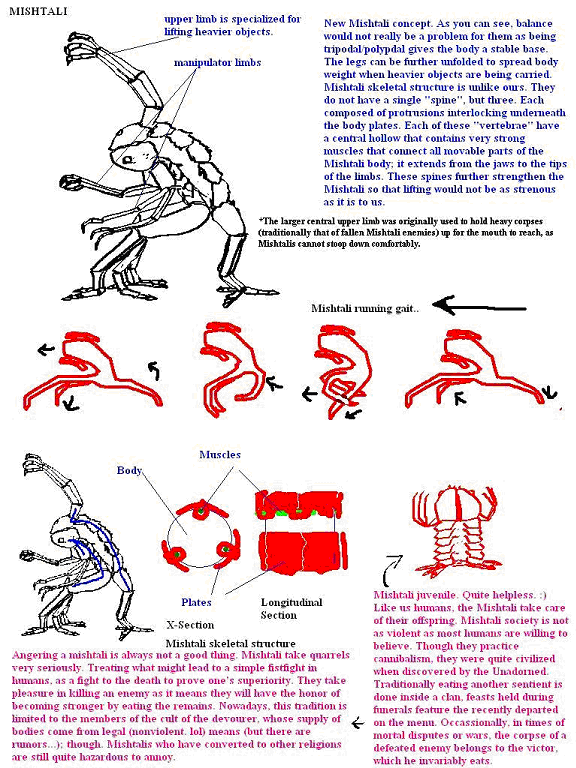
\includegraphics[width=0.75\textwidth]{images/Mishtali1.png}
}
    \caption{Mishtali}
    \label{fig:Mishtali1}
\end{center}
\end{figure}


\subsection{Habitat}
Oxygen-Nitrogen FIXME 

\subsection{Culture}
Given the cultural oddities of both the Unadorned, who come close to
religious reverence in their views on computers, and the Mishtali,
known for being the source of the Cult of the Devourer wherein the
religious rituals are accompanied by the consumption of the remains of
both Mishtali and alien sentients, it is believed by many to be just
as well that the Unadorned, as their discoverers, are responsible for
shepherding them.

\subsection{Religion}

The Mishtali practice a number of religions, both native and
foreign. Chief among the native religions in, albeit infamous,
notariety, is the Cult of the devourer. The Cult of the Devourer
centers on the belief that success in life is directly tied with what
one eats, and that the more powerful the being that was eaten, the
better one's life can be. Thus, eating the remains of sentient beings
is as good as it gets. This, obviously, raises a few issues among many
groups, but there are enough humans and Dgn willing to be paid for the
eventual consumption of their corpse that the churches of the Cult of
the Devourer tend not to lack for sustenance. These churches are, as a
rule, very festive and pleasant places to visit, provided one is not
turned off by the cuisine. The Mishtali have been very willing to
convert to just about anything, so the Mishtali also tend to have the
largest alien populations of most obscure human religions.

\subsection{Miscellaneous}
Base e.

This is what happens when math types (of admitedly questionable
initial sanity) decide to bring civilization to an undeveloped species
that doesn't understand exactly what is meant by "optimal".

\section{Nuhln}

\subsection{Physical characteristics}
Figure~\ref{fig:Nuhln} provides a clear depiction of a Nuhln.

\begin{figure}
\begin{center}
\makebox[\textwidth][c]{
    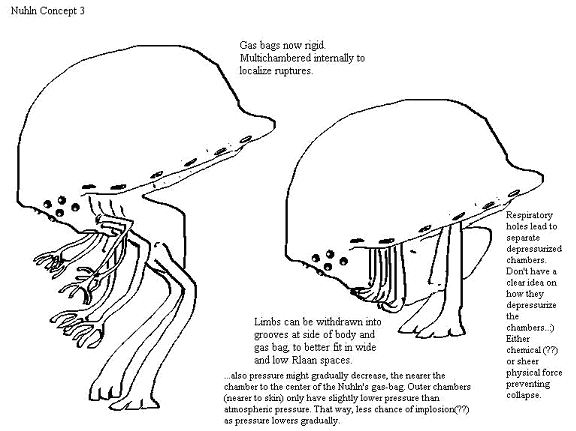
\includegraphics[width=\textwidth]{images/Nuhln.png}
}
    \caption{Image of a Nuhln}
    \label{fig:Nuhln}
\end{center}
\end{figure}

 
\subsection{Habitat}
Methane-Nitrogen 

\subsection{Culture}
Like the Lmpl, the Nuhln were a sub-sentient species selected by the
Rlaan for an uplift project. The first of the two major uplift
projects, the Nuhln are generally considered far less successful than
the Lmpl, being somewhat intellectually slow. They are almost
exclusively found performing jobs where the ability to repeatedly
perform seemingly mindless tasks without complaint is a distinct
positive attribute. Though present throughout Rlaan inhabited space,
they are a culturally subsumed group, possessing no internal culture
to speak of.

\subsection{Religion}
All Nuhln are adherents of Rlaanbzztkrlbzeentkaan (see ~\ref{Rlaanbzztkrlbzeentkaan}). 

\subsection{Miscellaneous}
The Nuhln use Rlaan numbers. 

\section{Purth}

The Purth are an uplifted client species of the Andolians. In large
part an experiment in synthesis of work done by the Unadorned and the
Mechanists, the Purth are cybernetic beings, with assistive AI and
built in networking capacity. It is only through these upgrades that a
Purth achieves something much like sentience.  Although they sometimes
operate autonomously from their Andolian patrons, Purth never do so
alone. Only by networking their minds together will a group of Purth
be confident enough to venture off without guidance.

\subsection{Physical characteristics}
The Purth were chosen primarily because of their very hardy
constitution, and have proved themselves invaluable in high gravity
applications. Each individual Purth is quite large, comparable to a
small motor vehicles, and covered in a skin heavily composed of
silicones. The silicones are at their most present on the footpads,
which allow the Purth to walk across still-cooling lava flows and
traverse boiling mineral springs.FIXME

\subsection{Habitat}
FIXME 

\subsection{Culture}
FIXME 

\subsection{Religion}
The Purth were pre-sentient before the Andolians altered them, and are
universally predisposed to ignore religious issues entirely.

\subsection{Miscellaneous}
Purth use binary, due to their number processing being heavily
computer assisted.

\section{Rlaan}

Ammonia-blooded, methane breathers from a cool world distantly
orbiting a hot star, the Rlaan are a collection of oddities. Unique
among the known space-faring groups, the Rlaan are actually two
separate species, the defenders and workers speciating some hundred
thousand or so years ago.

\subsection{Physical characteristics} 
{\em (Defender, Workers and Hybrids)}

Rlaan are radialy symmetric beings with a base four
split. Figure~\ref{fig:Rlaan-perspective} shows a perspective view of
a Rlaan from above. Their Workers (see
Figure~\ref{fig:Rlaan-worker-cutaway}) stand about one meter high at
the prime knee, and are nearly one meter in diameter. Members of their
Defender caste (see Figure~\ref{fig:Rlaan-defender-cutaway} for
cutaway image of Defender species) tend towards being 50\% larger in
both dimensions. Rlaan natively breathe a methane-based atmosphere,
and must wear special breathing apparatus to negotiate oxygen-nitrogen
environments. Their skeletal structure, being an exoskeletal carapace
supported internally by millions of reinforcing struts, is best suited
to lower gravity worlds, and leads to the use of mechanical assistance
on larger or denser rocky bodies.

\begin{figure}
\begin{center}
\makebox[\textwidth][c]{
    
\includegraphics[width=3in]{images/Rlaan-perspective.png}
}
    \caption{Rlaan - view from above and side}
    \label{fig:Rlaan-perspective}
\end{center}
\end{figure}
\begin{figure}
\begin{center}
\makebox[\textwidth][c]{
    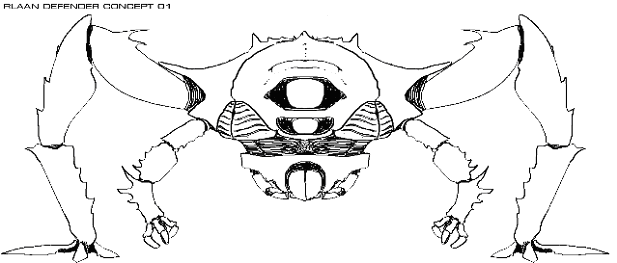
\includegraphics[width=\textwidth]{images/Rlaan-defender-cutaway.png}
}
    \caption{Rlaan Defender - front and back limbs omitted}
    \label{fig:Rlaan-defender-cutaway}
\end{center}
\end{figure}
\begin{figure}
\begin{center}
\makebox[\textwidth][c]{
    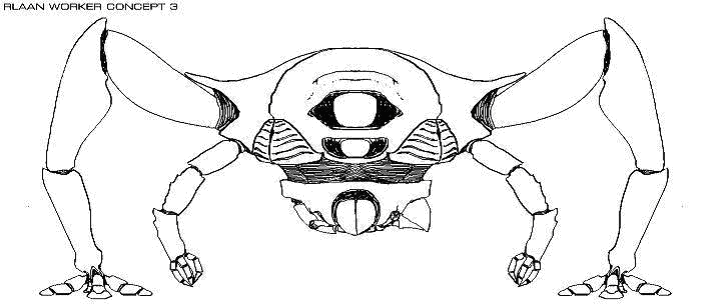
\includegraphics[width=\textwidth]{images/Rlaan-worker-cutaway.png}
}
    \caption{Rlaan Worker - front and back limbs omitted}
    \label{fig:Rlaan-worker-cutaway}
\end{center}
\end{figure}

Both species are similar in appearance, with the primary differences
being size, the degree of fine control in the manipulator appendages
(workers have better fine control), and the structural integrity of
the skeleton (defenders are less fragile than workers).  The defenders
tend towards darker shades of red and purple, whereas the workers are
somewhat pale. Though the offspring of worker-defender matings are
sterile, these hybrids exist as nearly 4\% of the population, and have
come to play important social roles, especially in the realm of
politics.  Rlaan are radially symmetric with four equivalent
segments. Each of these segments contains one compound eye composed of
four segments, one ambulatory appendage, one mouth with four
mandibles, one manipulator appendage, various local organs, and
portions of the central organs. The Rlaan skeleton is a supported
exoskeleton, that is to say, the exoskeleton is supported internally
by a network of millions of small extensions of the skeleton, which
together form a sort of highly porous lattice that the soft internals
reside in. A defender stands about 1.5 meters high at the top of its
carapace, and 2 meters high at its knee joint. The central body is
around one meter in diameter, and a third of a meter in thickness. Out
of this central body come the four abulatory limbs, going up and out
from the body to the knee joint, and then proceeding down where they
terminate in a four-splayed gripping foot. Suspended below the central
body is the "head" portion of the Rlaan, about half a meter in
diameter and also about a third of a meter in thickness, with its
bottom covered in a particularly thick extrusion of the
exoskeleton. The manipulator appendages sprout from the region
connecting the head with the main body, and end in four radially
arranged fingerlike structures. A worker's dimensions are about 70\%
that of a defender.

\subsection{Habitat}
With equatorial temperatures peaking near 230 K, seas of ammonia, and
a methane atmosphere, the Rlaan homeworld is not what most species
would consider a prime vacation spot. Life on this planet progresses
at a rather slower pace than that on water worlds, but proceeds
nonetheless. From the point of view of ammonia-methane life, the Rlaan
planet is actually quite toasty.

\subsection{Culture}
Rlaan lifespans tend to be between 250-350 years. This is believed to
be a large factor in their cultural homogeneity and the methodical
nature of their advances, both through space and as a culture. Rlaan
culture itself is a very dry affair, with social dynamics primarily
involved around expository investigations of philosophical debates
that have yet to be satisfactorily translated into the language of any
other species.

\subsubsection{Music}

Their music, if it can be called such, has been compared to "the set
of frequencies one would expect to register if a Myztherian Octpanther
were let loose in a campanile". On a more disturbing note, the Rlaan
central archives possess the largest collection of data concerning
Jerry Lewis and Yoko Ono outside of Human space. The Rlaan are,
however, regarded by many of the other space faring races as much more
intelligent than their culture's taste in art would suggest.

\subsubsection{Writing}

Rlaan written language appears as a sequence of characters consisting
of one to four radial slashes in each of four quadrants formed by a
pair of crossed lines. It is read in a counterclockwise spiral out
from a blank central region that is reserved for the signature glyphs
of the author. The Rlaan have vast stores of written documents going
back thousands of years, but attempts to decipher most of them have
met with limited success, as the concepts often being discussed seem
to have no corollaries in the languages of any other species.

\subsubsection{Science}

Rlaan science is more advanced in the fields of chemistry and genetic
manipulation than any of the other space-faring races. The Rlaan are
also quite knowledgeable about materials science and the advances in
the latter are often related to the former. Aside from these noted
cases though, Rlaan science has advanced more slowly than that of the
Humans or the Aera, and the extent of its advances is more a measure
of the age of Rlaan investigations into science than any particular
brilliance on the part of the Rlaan. Though not truly uncreative, the
Rlaan seem hard pressed in the department of inventive spontaneity. In
particular, the Rlaan are rather behind humanity in their exploration
of both artificial intelligence and tightly integrated biomechanical
systems, having sufficed with loosely coupled designer organisms.

\subsubsection{Politics}

The Rlaan are governed by a body whose name translates to The Rlaan
Assembly it appears to be some form of representative democracy, but
the exact methods of choosing one's representative seem complex and
arcane beyond the tolerance of most observers to bother attempting to
figure out. This body then churns out laws and regulations at a
breakneck pace, the enforcement of which is then delegated to the
complex Rlaan Bureaucracy. Attempts to understand the inner workings
of the Rlaan Bureaucracy have met only with confusion for all parties
involved. Strangely, the members of the Assembly are
disproportionately sterile hybrids, believed by the Rlaan to be more
levelheaded than either the aggressive defenders or the timid
workers. One thing that did translate clearly, however, was the Rlaan
differentiation between civilian and non-civilian. Given their
biological distinction between these two, it is easy to see why the
Rlaan have such firm views upon how civilians should be treated.

Notable Rlaan Factions and Organizational Entities
\begin{itemize}
\item The Rlaan Assembly 
\item Rlaan Briin 
\item Rlaan Merchants 
\item Rlaan Hunters 
\item Rlaan Enforcers 
\end{itemize}
\subsection{Religion}
\label{Rlaanbzztkrlbzeentkaan}
Most Rlaan are adherents of Rlaanbzztkrlbzeentkaan. What this means is
very difficult to say, as, though it is a text based religion, the
text is under constant revision. Indeed, the Rlaan Assembly regularly
submits changes and additions to the holy text. Contradictory edicts
abound, and scores of companion volumes are included with every copy
that debate the relative merits of breaking one set of edicts over
another. Edicts contradicting each other,however, are the least of a
reader's worries, as the universe is created 37 times in 17 entirely
distinct fashions, by a grand total of 4301 entities, albeit 4210 of
these were all in one creation story. History, morality, ethics, and
the fundamental nature of reality itself are all presented in so many
different forms in the text, that it defies rational understanding as
to how the Rlaan consider the book canonical and relevant. However,
they do. And they gather together at one of the 73 specified intervals
of worship, for those that interpret worship as being allowed, to
engage in whatever activity is currently believed to be both correct
and legal by the group that has thus met. Rlaan places of worship are
thus remarkably like most Rlaan art: constantly changing in nature but
composed of themes that are themselves mind-numbingly repetitive, and
constantly possessed of an aesthetic that runs counter to common human
tastes.

\subsection{Miscellaneous}
Depending on your viewpoint, the Rlaan use either base 4 or base
256. Namely, every Rlaan character is composed of 4 subcharacters, so,
going by the subcharacters, it's base 4, but there are 256 distinct
numerals per character read. Rlaan numbers are distinguishable from
the characters in the rest of the Rlaan script in that the center of
each subcharacter is marked with a dot. As far as the Rlaan are
concerned, it's base 256.

\section{Saahasayaay}

Fast, beautiful and deadly, while they serve the Rlaan, they do so
because of the technological and economic benefits gained from the
association rather than out of gratitude. Whereas the Rlaan succeeded
in making both the Lmpl and Nuhln useful and docile, the Saahasayaay
are indeed useful, but far from docile.

While the Saahasayaay are a single species in the technical sense,
their array of different metamorphic forms, each clearly of distinct
origins, is somewhat unique, and, as only certain of the forms are
possessed of any particular intelligence, and only one of accepted
sapience, in common reference "Saahasayaay" may often refer only to
the portion of the population in dominant sentient morphology.

The Saahasayaay have the strangest, and, on several levels, most
disturbing life cycle of any of the known extant sentients. Foremost
among its disturbing points is that the life cycle is clearly of
artificial origin external to the Saahasayaay homeworld. The
non-squeamish often find this more disturbing than the fact that
metamorphosis usually begins with the death of much of the body, and
proceeds via the semi-autonomous archival organ consuming what would
otherwise be the uneaten remnants of its own corpse to fuel its
generation of a new body. The archival organ, itself effectively
inedible, and encased in a protective shell, is not a native
feature. The organ features an absurd amount of unexpressed genetic
code - indeed, it contains genes describing thousands of species,
almost none of which are actually present on the Saahasayaay
homeworld. Indeed, the Saahasayaay appear to be the result of some
ancient (although not believed Ancient) xenoforming gone awry. Many of
the gene sequences present in the archival organ appear to be
irrevocably damaged or woefully incomplete, despite the presence of
significant error correcting facilities.

Only the lowest level of the metamorphic chain for the Saahasayaay can
actually breed. All other forms have been rendered sterile. This
lowest level is a fast growing photosynthetic invader species that has
infiltrated or replaced competitors in most of the native ecosystems
of the Saahasayaay planet. It cannot be correctly termed a plant,
animal, or fungus, although it shares some features with all of these
more familiar categories. While likely originally designed to be the
prime xenoforming agent for the planet, destroying native ecosystems
and replacing them with those of its creators, the archive creeper has
wandered from its original mission, producing a warped hybrid
ecosystem that almost certainly bears little resemblance to either the
original or intended replacement. The origins of the Saahasayaay are
clear in both their metamorphic paths, their traditional food chains,
and the sterility and monosexual nature of all of the extant forms
save for the archival creeper. Local "herbivores", for lack of a
better word, came to eat the creepers, but were in turn recorded and
replaced, themselves devoured and recreated by the archival organs
they attempted to consume. This effect then proceeded to trickle up
the food-chains of all of the ecosystems invaded by the creepers. A
limitation of this process, was, of course, that organisms smaller
than the archival organ were not readily assimilated. Thus, the
detritus feeders competing for flesh on the fallen corpse of an
assimilated species were more likely eaten by the archival organ than
the other way around.

The archival organ is an incredibly complex, advanced, and subtly
broken biological machine, but it is not itself remotely
intelligent. Likewise, it is not quite sufficiently autonomous to
generate widespread agreement as to it being referred to as a
symbiotic organism, especially as the genetic definitions are skewed,
given that it contains all of the genetic code for all of the "host"
bodies. All tissues in the archival organ feature cellular
immortality, and the archival organ is itself amortal (not aging, nor
dying from old age) although the bodies it produces do not share these
properties. The organ is well protected and possesses some independent
subsystems, so surviving the death of the rest of the body is common
(depending on the manner of host-death) - which is necessary, given
that such is the only means for morphological change and the
preservation of more interesting forms of species. The archival organ
plays key hormonal regulatory roles in all of the assimilated forms.

\subsection{Physical characteristics}
Terminal form Saahasayaay are physically impressive beings, if not,
because of mode of movement, as bulky as some of the other sapients,
and fossil records indicate this to be a quality preserved from
pre-assimilation times. They are beautiful, if possessed of features
that, if designed, would speak of a certain viciousness to the
crafting hand. The terminal Saahasayaay are the only extant sophonts
known to be able to fly, albeit they are, in practice, more often
gliders than active flyers through their thick and caustic
chlorine-nitrogen atmosphere. Their bodies are long, almost
serpentine, though the strong muscular development for the wings and
arms belies that image. They are bilaterally symmetric, with 4 wings
rising above, and 8 arms hanging below the largest and middlemost
segment of the body, set between a long tail at rear and longish neck
and fierce head at front. The front and rear sets of arms have
hand-like endings, gripping appendages of a gaunt leather-and-bone
appearance, that are dexterous, if clearly meant to hold fast to live
and struggling prey while the curved blade-like endings of the middle
four arms carved and scooped the meal into edible submission. Skin on
the middle-body is mostly hidden behind large, thin, overlapping
scale-like protrusions of smooth, hardened flesh, iridescent, ranging
through colors from green to red to gold. The tail, in cross section,
could be thought of as a square whose sides have been bent in, or
whose corners were pulled out, to produce a four-sided concave
shape. The tail is heavily segmented, as is the neck, which has a
similar shape, although much larger, and it lacks the short spines
protruding from the corners of each tail segment that serve to let the
tail be used to grip surfaces or objects it has been wrapped
around. The tail narrows somewhat as it progresses rearwards, but was
always fairly thin in comparison with the body. Towards the rear of
the tail, the spines end, and four specialized spines are present that
act as fins that can be raised or lowered to act as flight control
surfaces. The scale-like protrusions are much larger on the tail and
neck than on the body, corresponding heavily to the structure of the
segments themselves leaning somewhat towards a more chitinous-plates
appearance than scale-like appearance, for those portions, although in
truth it is only a matter of size and flexibility required for each
segment that has lead to the differing appearance, and not a
fundamental change in material. The head is slightly larger in girth
than the neck, excepting the mouth itself which is forward of the rest
of the head. The terminal form Saahasayaay have no teeth in their
mouth. Grinding, separating and pulverizing are instead done by
stone-hard protrusions that line their equivalent of the
esophagus. The mouth instead consists of a set of flexible, segmented
spines, connected to each other by membranes, that can be focused to a
point, as when sucking in fluids or flying, or opened to engulf a
portion of a prey animal. This semi-engulfing is necessary, as the
chunks of flesh freed from the target by the multiple bone-bladed
tongues that slash out violently from within the mouth might otherwise
fall out. There are four eyes, two at the corners of the top of the
head and two, more centered, below. There are ears and nasal openings
that lie on the side of the head. The brain itself is primarily on the
top of the head, although there is significant neural matter at the
bottom of the head that does optical processing for the lower eyes.


\subsection{Habitat}
All of the native species integrated by the archival organ are now
extinct. Thus, entire food-chains now consist of nominally Saahasayaay
organisms. It is presumed, given that all of the non-creeper
morphologies are sterile, that the intended process involved a
kill-off of all of the food-chains via a wave of progressive
morphology changes up the food-chain, thereby progressively starving
each link in the chain. Alternate theories presume an external agent
being introduced that would kill off all of the hybridized life forms,
while leaving the invaders intact, but the non-native codes are
sufficiently mangled that it has been difficult to test if such
differentiation would have been readily achievable. Given the large
number of codes stored, it is presumed that total kill-off was not an
intended goal. Clearly, however, none of these have happened,
especially those models requiring external intervention. Instead, the
regulatory mechanisms presumably in place to delay any native
depopulation until there has been sufficient infiltration of the
native populations have instead functioned merely to regulate the
frequency with which the next body of a dead Saahasayaay differs from
the previous. Also noteworthy is the terminal nature of the
Saahasayaay metamorphic process. Fossil records point to the ancestor
of whatever native species preceded the sapient Saahasayaay population
as having been wide-ranging, and wherever present, atop the food
chain. Thus, the Saahasayaay sophonts are currently the "terminal"
metamorphic form - an archival organ that survives a Saahasayaay
sapient's death will normally build another Saahasayaay sapient. Note
that none of the previous individual's memory or mentality is
preserved, and inefficiencies in conversion and the genetic
imperatives of brain development in the original source species, even
in the presence of a nearly full corpse, result in the production of a
juvenile individual.


\subsection{Culture}

The most successful of the Rlaan client species, the Saahasayaay are
not, unlike the Nuhln and Lmpl, true uplifts, having already achieved
some minimal level of societal advancement at the point of discovery.

The Rlaan have taken to using Saahasayaay troops to reinforce their
border with the Aera, are, however, somewhat hesitant to let this
concentration of troops return home.

As most of the Saahasayaay forms are not capable of complex thought,
they don't much consider either the nature of their life cycle, nor
that they often are eating what is technically a member of their own
species. This is not the case for terminal form, whose culture has
been deeply shaped by the role that death plays in the Saahasayaay
life-cycle, and the semi-reincarnations that are the daily occurrences
of Saahasayaay life. The terminal form Saahasayaay are, in fact, quite
bright, and learn voraciously, but a cultural disinterest in knowledge
unrelated to superior killing ability and an exceptionally low
life-expectancy rate due to unending war, murder, and ritual killings
has historically hampered internal sources of advancement. It is not
too difficult to see where their obsession with death has come from,
albeit only they, perhaps, can truly comprehend the directions it has
taken them in. It is fortunate for all other sapient species in the
region that the Saahasayaay were found in the stone-age by
space-faring sapients, and not the other way around, as the
Saahasayaay have no compunction when it comes to killing, whether it
be other sentients, each other, or lower Saahasayaay forms. Death is
the natural order for them, it is the source of progress, and their
right and duty to disperse. Their obedience to the Rlaan and restraint
in aggression against both the Rlaan and other species is predicated
on the Rlaan's greater ability to bring death upon them than they upon
the Rlaan, as well as the opportunity for greater empowerment that the
Rlaan bring to the Saahasayaay. Death is the ultimate blessing the
Saahasayaay believe they can bestow, and the frequent regeneration of
their fallen into newborns has utterly deprived them of the fear of
their own demise present in all other known organized species of
measurable intelligence.

Some of the other Saahasayaay forms possess some level of
intelligence, though none as pronounced as the terminal form
Saahasayaay. Some of these forms have been "domesticated" and the most
intelligent of these, generally considered comparable to some of the
Terran primates, are sometimes used in a servitor role. The most
valued of the servitors are granted a chance at "ascension" by being
taken to an isolated area, free of terminal Saahasayaay, and killed
swiftly, leaving the entire corpse intact. The lack of terminal
Saahasayaay in the area improves the likelihood that the next
metamorphic form will be a terminal Saahasayaay, rather than another
servitor, as the choice of next form is heavily influenced by the
presence of other forms detected by the archival organ, a
manifestation of its original, more overarching regulatory
role. Punishment in terminal Saahasayaay society rarely involves
killing of the archival organ, an act considered disgraceful unless
the individual in question has been deemed to be heretical to the
advancement of the Death God's agenda, but it almost universally
involves killing. Punishments range from the minor, a swift and clean
death followed by adoption for what most other species would consider
misdemeanors, to use as hunt bait and eventual consumption by lower
forms, to the most serious crimes being punished by the removal of the
archival organ, the starvation thereof for a period of time, to
increase the chance of form reversion, smearing the archival organ in
the mixed remains of lower forms to further increase the odds that the
next form will not be a terminal Saahasayaay, and then letting the
starving archival organ eat the victim (still conscious, but wracked
with crippling chemical imbalances) alive.

It is generally considered fortunate that only a small percentage of
the world known to be reachable via the jump network feature a
chlorine based ecology. The Saahasayaay, from the creeper on up,
feature a profoundly rapid metabolism, and they have quickly overrun
and populated other chlorine-worlds that they have been introduced
to. Indeed, it has long perplexed researchers as to why exactly the
concentration of chlorine-life friendly worlds is significantly higher
in the region of space containing the Saahasayaay homeworld, and then
marginal elsewhere. What many believe to be the likely originating
planet of the archive creeper is in very nearby space, just one jump
link removed from the Saahasayaay system, but it is difficult to
ascertain this connection with any certainty. The system shows signs
of previous habitation by a technological entity, but, outside of
semi-preserved ruins on various moons and other uninhabitable
locations, there is precious little left of the inhabitants. In
particular, what is believed to have been their homeworld would seem
to have fallen victim to both some sort of limited grey-goo event and
a widespread use of fusion, antimatter, and kinetic weapons that,
combined with the already reactive nature of the atmosphere, served to
make it exceptionally difficult to discern much about the previous
inhabitants. Levels of nano-plague are also exceptionally high in the
system, leading several researchers to advance theories that the
inhabitants made what proved to be a fatal mistake of attempting to
counter the nano-plague in an aggressively military fashion.

The Saahasayaay navigate 3D space with great agility, and, despite the
distinctly different dynamics of planetary and vacuum flight, make
excellent pilots in either medium. The Saahasayaay have not
significantly industrialized on their own, although their
technological usage has greatly advanced since absorption into the
Rlaan Assembly. All Saahasayaay ships are specially manufactured for
them by the Rlaan out-system, and Saahasayaay pilots shipped out to
military bases from one of the Saahasayaay worlds. The Rlaan are
somewhat reticent when it comes to providing the Saahasayaay with a
means to make their own starships. They are, however, more than
willing to freely give them technologies which increase their
sustainable populations so that they can draw upon more Saahasayaay
troops. The Saahasayaay, for their part, hunger for more control over
their own destiny, but are currently kept sated with the opportunity
to bestow much bigger deaths with the starships the Rlaan build for
them (the Saahasayaay consulting on certain aspects of the
design). Saahasayaay operating in Rlaan space must wear
atmosphere/temperature suits at all times, precluding flight
abilities. Their suits are therefore augmented with thrusters so as to
make them more comfortable - an uncomfortable Saahasayaay is not a
safe Saahasayaay, though there is of course, no such thing to begin
with. Saahasayaay work only with defenders and hybrids in Rlaan
society. They have no respect for the Rlaan workers, who cannot be
killers in any meaningful way, and the Saahasayaay are considered an
unnecessary threat in interacting with Rlaan workers.

\subsection{Religion}
The dominant belief structure of the Saahasayaay revolves around each
of them being an intruments of the great death god who sits in
judgment over the universe. The Saahasayaay belive themselves to be
the chosen people who alone are privy to the sentences being passed
down upon the mortals of this realm. Saahasayaay prophet halls are
built to express the joy of the hunt, the glory of the kill, and
subserviance to the great death god. The prophet halls are built in
keeping with the 3-dimensional nature of Saahasayaay travel, with
perches on many levels, and rank denoted by attainment of a higher
perch.

\subsection{Miscellaneous}
The Saahasayaay used to use a unary system with groupings done in sets
of 8 (flat, without a notion of base), but have been converted to use
of the Rlaan base 256 system.

\section{Shmrn}
\label{subsec:Shmrn-species}
The Dgn and Shmrn share a common time-of-uplift ancestor. The
resulting species was further refined in seperate efforts by the
Lightbearers and the Shapers into two distinct, but closely related
species. As the Lightbearers were destroyed as a meaningful entity,
the Shmrn were let loose as a freed species to settle new worlds.

\subsection{Physical characteristics}

\subsection{Habitat}

\subsection{Culture}

For above 3 categories, please see the following list of images: Figures \ref{fig:Shmrn-overview}, \ref{fig:Shmrn-ancestral}, \ref{fig:Shmrn-elder}, \ref{fig:Shmrn-medic}, \ref{fig:Shmrn-pilot}, \ref{fig:Shmrn-pilot1}, \ref{fig:Shmrn-footwear}, \ref{fig:Shmrn-formalwear}, \ref{fig:Shmrn-logo}, and \ref{fig:Shmrn-render}.

\begin{figure}
\begin{center}
\makebox[\textwidth][c]{
    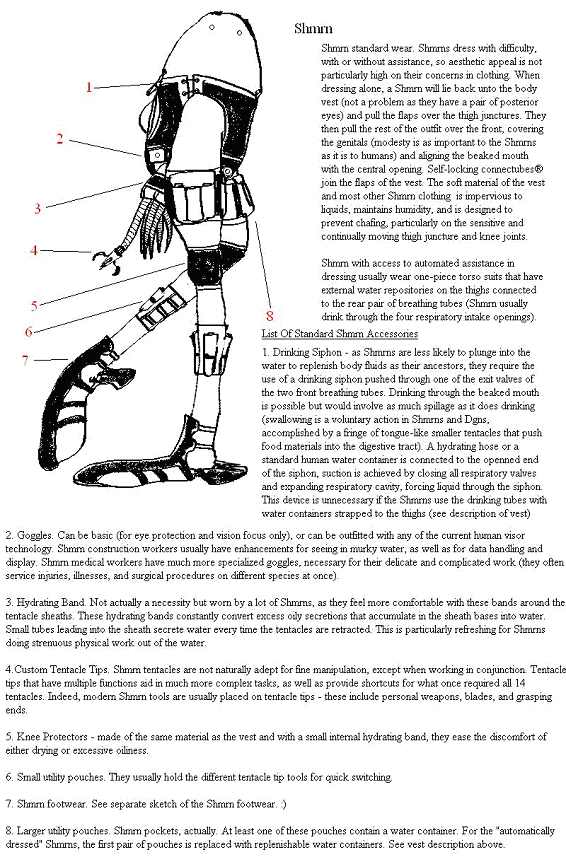
\includegraphics[width=0.75\textwidth]{images/Shmrn-overview.png}
}
    \caption{Shmrn Overview}
    \label{fig:Shmrn-overview}
\end{center}
\end{figure}
\begin{figure}
\begin{center}
\makebox[\textwidth][c]{
    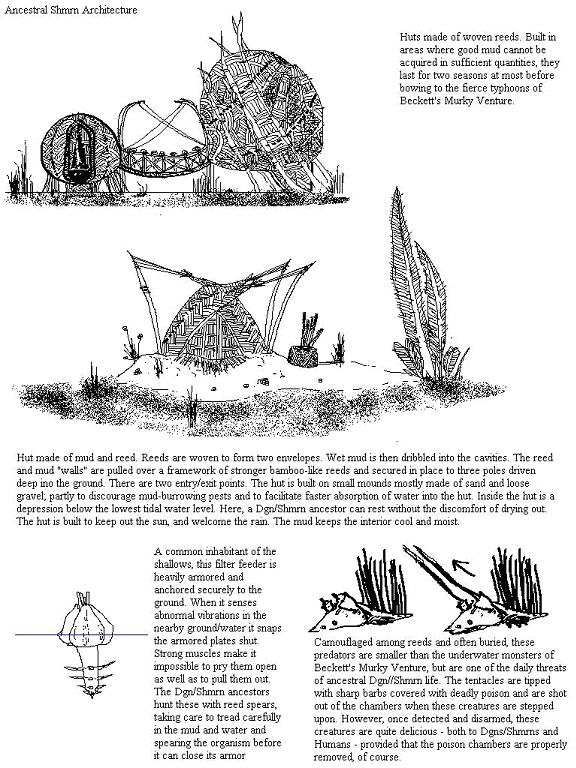
\includegraphics[width=0.75\textwidth]{images/AncestralShmrnArchitecture.png}
}
    \caption{Habitat of the ancestral Dgn/Shmrn}
    \label{fig:Shmrn-ancestral}
\end{center}
\end{figure}
\begin{figure}
\begin{center}
\makebox[\textwidth][c]{
    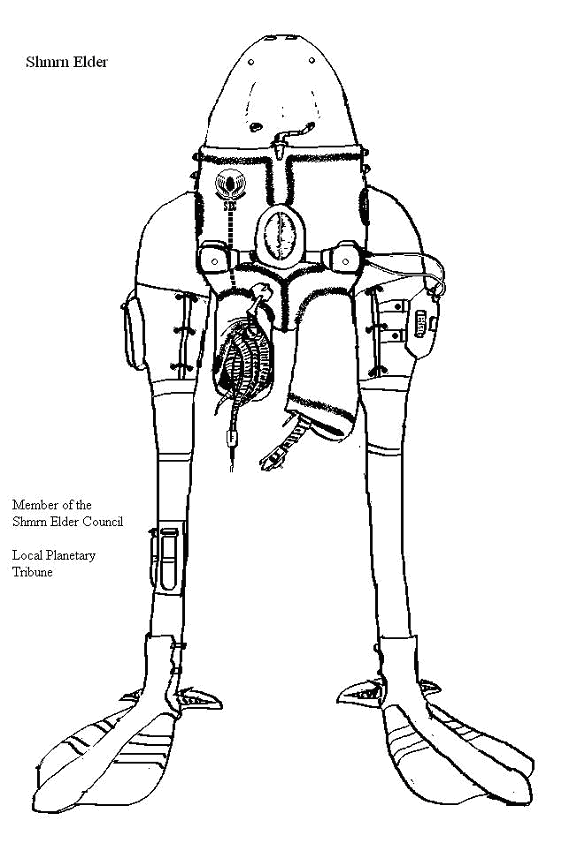
\includegraphics[width=0.75\textwidth]{images/Shmrn-elder.png}
}
    \caption{Shmrn Elder}
    \label{fig:Shmrn-elder}
\end{center}
\end{figure}
\begin{figure}
\begin{center}
\makebox[\textwidth][c]{
    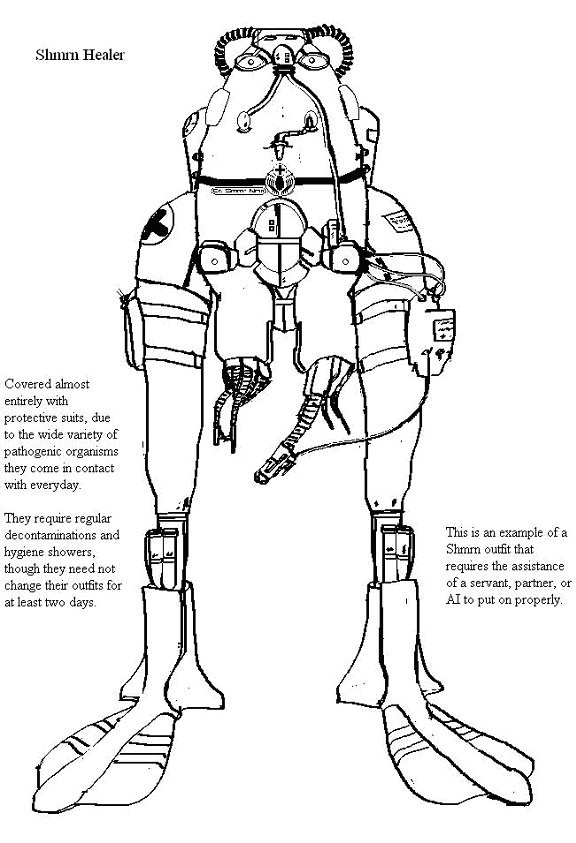
\includegraphics[width=0.75\textwidth]{images/Shmrn-medic.png}
}
    \caption{Shmrn Medic}
    \label{fig:Shmrn-medic}
\end{center}
\end{figure}
\begin{figure}
\begin{center}
\makebox[\textwidth][c]{
    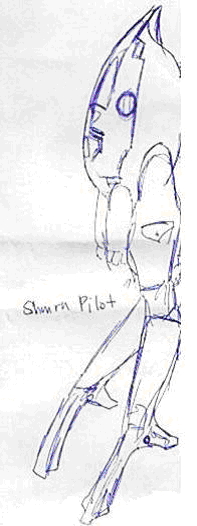
\includegraphics[width=0.25\textwidth]{images/Shmrn-pilot.png}
}
    \caption{Shmrn Pilot(1)}
    \label{fig:Shmrn-pilot}
\end{center}
\end{figure}
\begin{figure}
\begin{center}
\makebox[\textwidth][c]{
    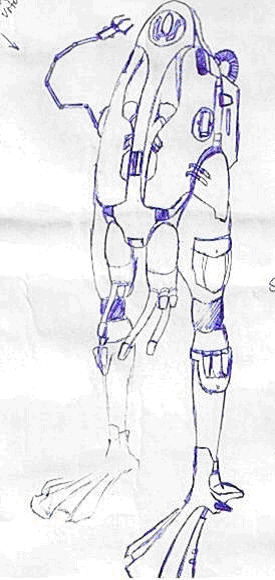
\includegraphics[width=0.25\textwidth]{images/Shmrn-pilot1.png}
}
    \caption{Shmrn Pilot(2)}
    \label{fig:Shmrn-pilot1}
\end{center}
\end{figure}
\begin{figure}
\begin{center}
\makebox[\textwidth][c]{
    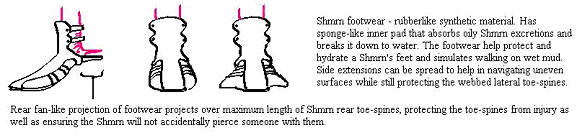
\includegraphics[width=\textwidth]{images/Shmrn-footwear.png}
}
    \caption{Shmrn footwear}
    \label{fig:Shmrn-footwear}
\end{center}
\end{figure}
\begin{figure}
\begin{center}
\makebox[\textwidth][c]{
    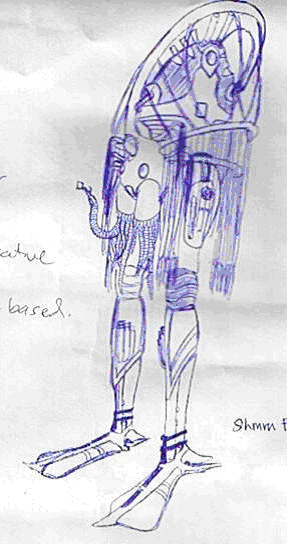
\includegraphics[width=0.5\textwidth]{images/Shmrn-formalwear.png}
}
    \caption{Shmrn formalwear}
    \label{fig:Shmrn-formalwear}
\end{center}
\end{figure}
\begin{figure}
\begin{center}
\makebox[\textwidth][c]{
    
\includegraphics[width=2in]{images/Shmrn-logo.png}
}
    \caption{Shmrn logo}
    \label{fig:Shmrn-logo}
\end{center}
\end{figure}
\begin{figure}
\begin{center}
\makebox[\textwidth][c]{
    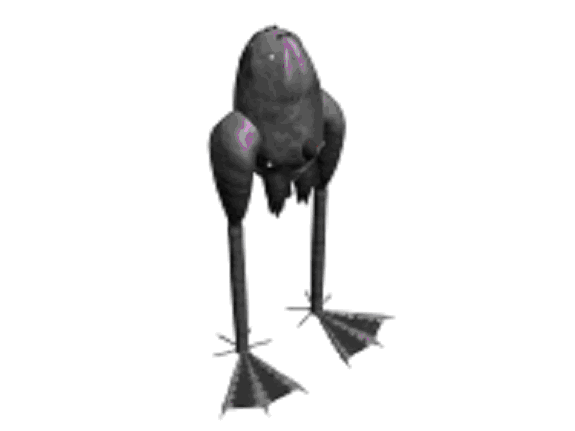
\includegraphics[width=\textwidth]{images/Shmrn-render.png}
}
    \caption{Shmrn - rendered}
    \label{fig:Shmrn-render}
\end{center}
\end{figure}

\subsection{Religion}
The Shmrn have a spiritual existence quite different from their
brothers the Dgn, with communal meetings contemplating the nature of
suffering over one's lifetimes dominating the organized religious
landscape. Shmrn culture and universe view centers on the principles
that life is unfair and painful, but a necessary stage to receive the
reward of eternal painlessness that awaits those who have, over
several lifetimes, overcome their desires to avoid the unpleasantness
of life.

\subsection{Miscellaneous}
Base 7. Nothing special. 

\section{Super Cetaceans (SuCets)}

Super Cetaceans (SuCets) are the result of what some consider the
first truly profound endeavours of Humanity in combining the fields of
genetics and cybernetics. While there are still SuCets around, they
are generally considered a "failed" experiment, never thinking in a
sufficiently compatible manner to become either useful tools or
partners, and requiring cybernetic additions that were too costly,
post nano-plague, for novelty value. Small communities of SuCets exist
on some of the more affluent and metropolitan oceanic worlds, and
their largest community, though quite small, remains on Earth.

\subsection{Physical characteristics}
The bulk of their genetic code derived from a potpourri of whales and
porpoises, they are oxygen breathing swimmers of immediately
recognizeable cetacean form, overcoming their lack of manipulator
limbs via integrated mechanical prosthesis.

\subsection{Habitat}
The shallower seas of the continental shelves and the vast waters of
oceans and oceanic worlds with oxygen-nitrogen atmospheres.

\section{Super Simians (SuSims)}

Super Simians (SuSims) and SuSim Cyborgs have been one of the more
stunting trends for "true" AIs, arising from the advances in the
fields of genetics and integrated cybernetics. For physically
manifested tasks considered too menial, too dangerous, or too
monotonous for Humans, the SuSims and SuSimCys proved cheaper, more
reliable, and, through advancements in genetics, easier to dominate
than AI alternatives.

As a client race they are quite prevalent in High-Born space as
servants. In other societies, however, the use of SuSims is seen as
inhumane or otherwise frowned upon.

\subsection{Physical characteristics}

The SuSims were constructed from augmented blends of Terran primates,
and many discernable features of their Chimpanzee and Bonobo ancestors
are immediately recognizeable. They remain hairy, not for practical
purposes, as much as to help convince their masters that the lines
between pet, tool, and slave have not been crossed in an era when some
"Humans" may be further distant genetically than the SuSims are from
Homo Sapiens Sapiens.

\subsection{Habitat}
They are capable of breathing an oxygen-nitrogen atmosphere. 

\section{Those who have only names (TWHON)}

What little is described of this group is gleaned from writings left
behind by the Ancients. While most descriptions are quite vague, it is
clear that TWHON, if the Ancients are a reliable source, were at least
as advanced as the Ancients, and much older.

\section{Uln}

FIXME 

\subsection{Physical characteristics}
 
8 limbs, 4 legs, 4 arms. Each arm end in a "hand" with 4 "fingers" one
of which is opposable. The four legs terminate in fleshy-padded feet,
each of which ends in sets of broad, thick, fore and back claws
capable of allowing "tree"-climbing. All four legs are visible in the
rear picture (this specimin has somewhat skinny front legs). The two
arm pairs are socketed between the two leg pairs, one pair of arms
reaching over the head, the other coming up from under. The head is
large and block-like, situated on a short, muscular stalk of a neck
protruding from the main torso. The main torso features twin rows of
breathing holes, visible on the back/underside.

There are 3 moving parts in the Uln jaw, a lower jaw, and two side
portions, all of which are normally involved in eating. There is a
single visual input band that stretches across the front and onto the
sides of the Uln head, forming a cover for their complicated compound
eye. Uln vision is actually remarkably good, and they can see from the
infrared/near-microwave into soft UV (hence, some interesting trends
in Uln clothing materials).

Figure~\ref{fig:Uln-bodyplan} sketches the basic shapes described above.

\begin{figure}
\begin{center}
\makebox[\textwidth][c]{
    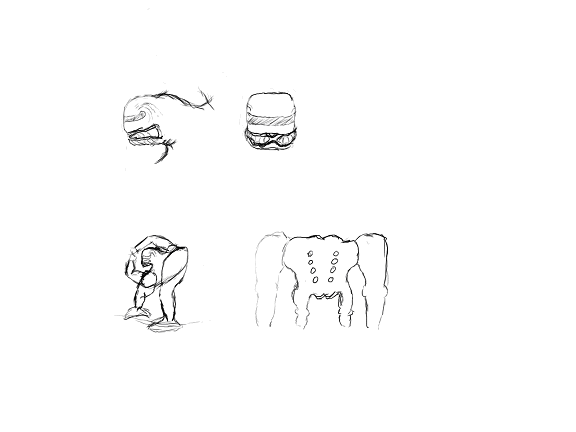
\includegraphics[width=\textwidth]{images/Uln-bodyplan.png}
}
    \caption{Partial sketches of Uln body plan, details of head.}
    \label{fig:Uln-bodyplan}
\end{center}
\end{figure}


\subsubsection{Digestion}

The Uln don't do well with carbonated beverages. At all. Their
digestive tract isn't suited to things that expand that rapidly upon
consumption, and they will make a horrid, stinky mess of things when
they exhibit that gem of convergent evolution (traditionally for toxin
removal) of spewing their food back out.

\subsection{Habitat}
FIXME 

Oxygen-Nitrogen.

       (Shmrn logo)


\subsection{Culture}
The Uln culture sprang up among the remains of a sprawling set of
Ancient structures and advanced in technology faster than their
biology or social structures could adapt, leading one noted human
researcher to note upon seeing them, "It was as if I had suddenly come
across a spacecraft piloted by Homo Erectus -- if they hadn't been so
ill prepared for the gifts they unintentionally received, they would
have conquered the entire arm." Fortunately for the aspirations of
dominance held by other species, the Uln were decidedly
unprepared. Indeed, they spent so much time blowing each other up with
weapons they didn't entirely control that it is a wonder that either
they or the ruins on their planet still survive.
\begin{itemize}
\item History

Uln development is somewhat difficult to follow, as they are not
actually "native" to their homeworld. Indeed, very little of the plant
and animal life on the entire planet appears to have been of native
origin, present for only millions of years. In particular, the species
on the planet appear to have come from many different origins, as is
sensible given the broad range over which Ancient sites have been
discovered in other star systems. The Uln are not generally very
talkative about their origins, especially as it is the common
agreement among the other sapients that they're the descendents of
whatever the Ancients were using for lab rats/monkeys. It is therefore
still a matter of some debate as to which features of the Uln are
naturally occurring, which were engineered, and what reasons there
were for such choices.

\item Clothing

The most commonly worn Uln garments range from "open-toed(clawed)"
short-boots, some utility pouches with straps around the upper arms
resting on the neck, and a helmet-scarf (draping down to cover more
sensitive regions between the underside of the neck and the lower
arms) which would be common casual-wear for the common peon, to the
foul-weather knee-length boots and helmet-poncho and the bizzare
extravagances of the aristocratic class, with gaudy creations not
unlike wearing an array of very fine wire-meshes and doilies, that
require servants to dress them. The back/underside is not normally
overly covered, though something may drape loosely behind the top arms
- to do otherwise would interfere with their breathing.
\end{itemize}
\subsection{Religion}
Growing up amidst the ruins of an exceptionally powerful and ancient
culture on a planet where life was artificially introduced gave the
Uln the idea that they were the children of failed gods. Convincing
them that they are much more likely the descendants of
lab-monkey-analogs from a long destroyed outpost hasn't gotten very
far. What passes for organization in Uln religion involves seasonal
festivals that mostly serve to reinforce the doctrinal line that being
born Uln is a wonderful thing, relative standard of living to the
other species be damned.

\subsection{Miscellaneous}
Base 4. Nothing special. 


\clearpage
\stepcounter{appendixcounter}
\refstepcounter{chapter}
\section*{Appendix \Alph{appendixcounter}: Faction information}
\addcontentsline{toc}{chapter}{Appendix \Alph{appendixcounter}: Faction information (In-game Viewpoint circa 3276 CE)}
FACTIONS of the UTCS Time Period


FIXME

§	Confed IntelSec 
o	Confederation Navy 
o	Exploratory Service 
o	Concerned Confederation Citizens Against the War 
o	Confed Pleasure Planet Travel Consortium (CPPTC) 

\section{Aeran Ascendancy}

The Aeran Ascendency governs the Aerans and Bzbr. The Aeran Ascendancy
is, in practice, a body wholly controlled by entirely Aeran will of
the Aeran Oligarchy. All distinct Aeran subgroups, such as the Aeran
Merchant Marines are subject to the edicts of the Aeran Oligarchy.

\subsection{Aera}
Faction data 
Aera 
Species 	Aera 
Homeworld (Origin) 	Aeneth 
Capital 	Aeneth 


\subsubsection{A Brief History of the Aera}

The Aera homeworld was home to extremely competitive ecosystems. It
was not a supportive environment. If one considers Earth the "mother"
of the human race, then, in comparison, Aeneth was an abusive
parent. The Aera evolved in an environment where a slew of things
really did want to kill/eat/infest them. Beginning with the early
harnessing of fire, and ending with industrial might, the Aera
remedied this problem by destroying the vast jungles that bore
them. However, their outlook on the universe was fundamentally shaped
by their beginnings in a direction that humans would consider
paranoid, or at least profoundly pessimistic and somewhat untrusting,
though the Area merely see it as prudent recognition of how the
universe works.

This outlook was greatly reinforced by the Aera experience with the
nano-plague. The precocious Aera, unlike humans or Rlaan, developed
jump-based FTL before having otherwise left their solar system. The
resultant reactivation of the nano-plague and the devastation it
wrought on their population, served to gel their concept of an
inherently antagonistic universe. Aeran society greatly increased its
militarization, heretofore on the wane since global unification, so as
to better prepare for potential conflicts in what, evidenced by the
nano-plague, they presumed was an inhabited galaxy.

The Aera are the youngest of the three currently dominant space-faring
major groups, but are also the most expansionist, fastest breeding,
shortest lived, and devote the highest fraction of their economy to
military and military related R\&D spending. They are not evil, they
are not delusional, they are not irrational, but they have some
fundamentally different assumptions they are working from that make
them somewhat difficult to get along with. Finding out that their
section of the jump network had them pinned by the Humans and Rlaan,
they first attempted to negotiate passage, and were rebuffed. They
then attempted to sneak a colony convoy through Rlaan space, but this
turned into an utter debacle after Aeran escorts killed Rlaan
Civilians, sparking a war lasting several years, that churned the
Rlaan-Aeran border into an abattoir. Although formal peace has never
been brokered between the two, a cease-fire has been in effect for
several years. The Aera have now turned their sights toward Human
space, invading Forsaken territory, hoping to push through toward the
less defended Forsaken/Confederation border crossings, carve a
corridor through to the other side of humans space, and keep it open
long enough so that they can send enough colonization fleets through
to the other side to make the venture worthwhile.

\subsubsection{Development}
Compared to contemporary 33rd century humans, the Aera are comparable
or somewhat more advanced in some of the physical sciences and their
applications, notably so with respect weaponizations of certain
technologies. They are noticeably behind in life sciences and AI.

Having been wandering the jump network for the least amount of time
(among the Rlaan/Humans/Aera), the Aera, though occupying the same
order of magnitude of systems as the Humans or the Rlaan
(Rlaan/Lmpl/Nuhln/Saahasayaay have most, followed by
Humans/Klk'k/Dgn/Purth/Mishtali, followed by Aera/Bzbr, then the much
smaller Uln, Shmrn) have not occupied many of them for nearly as
long. The Aera expanded in territory faster than that territory could
be developed up until running into the Uln. After one last push then
brought them to the Human and Rlaan borders as well, the Aera have
been racing to build up their newly settled colonies nearer the
borders, but the bulk of their industrial potential remains
concentrated in systems closer to their homeworld than to alien
space. This difference was especially clear during the Rlaan-Aera
conflict, wherein many newly settled Aeran colonies along the border
fell to the Rlaan assault, but the same Rlaan fleets were badly
bloodied when they tried to push into Aeran systems with more matured
defenses. Due to the war, Aeran military spending and infrastructure
development has been extravagant in comparison to human budgets, but
the Aera also had to cope with sizeable losses in personnel and
materiel.

While there are key differences between the level of population and
industrial development between the core colonies and the newer
colonies, due to the very strong central organizing forces in Aeran
governance and economy, this is not a deep political divide, nor an
economic one - it is merely a matter of the more fringe planets
growing as fast as they can into states undifferentiable from the more
core worlds. This centralization should not be taken as evidence that
Aerans are a selfless society of collectivists. Rather, the Aera have
a strong natural ability and desire to sublimate personal interests to
higher authority, a trait left over from their more pack-like
origins. Success, however, is still judged at individual granularity,
and Aera are entirely opportunistic about personal advancement when
the opportunity either does not come at the expense of the dictates of
higher authority, or places them into a position of higher authority.

\subsubsection{Culture}
The Aera are a bit culturally dour, although they do engage in
organizational events, such as rallies, sporting contests, and
Military parades. Entertainment pursuits, such as music, for personal
pleasure are not a significant thread in Aeran culture. Such pursuits
are seen as necessary avenues of release, but to devote oneself to
pursuing purely entertainment oriented activities merely because they
are pleasant is seen as wasteful, wantonly hedonistic, and a reckless
abandonment of one's duties. Entertainment with physical components,
such as sporting competitions, are viewed in a more favorable light.

In Aeran culture, mortality is to be pondered and meditated upon in
its inevitability. It is worth noting that it is not so much those
that came before them that the Aera cherish as the accomplishments of
those who came before them. The Aera perspective is that it is only
though accomplishment on behalf of the Aera that the Aera can
continue, and the dead, thereby, can continue to live in the memories
of the Aera.

\subsubsection{Organization}
Aera culture is highly organized and decidedly hierarchical, but in
the form of a meritocracy rather than an aristocracy. While what has
constituted merit has morphed over the millennia since the first Aera
tribes selected work crews to cut back the encroachments of the jungle
upon their early settlements, given the relative position of the
pre-technological Aera in their local food chain, there has long been
a favoring of cleverness and determination over raw strength. The
current social and vocational position of any Aera is immediately
indicated by the color and pattern of an individual's coverall. The
Aera are ruled by a subset of the highest caste, with membership in
the oligarchy changing whenever either an individual steps down, or a
third of the other members call for a member's replacement. New
members must be confirmed by two thirds of the current oligarchy. It
is much more common for members to voluntarily remove themselves from
power, believing themselves more useful elsewhere in society, than to
be cast out. An average stay in the oligarchy lasts a few Aera years.

Need to more usefully carve up faction vs. species information. Will
do so later.FIXME

\subsection{Aeran Merchant Marine}

Faction data 
Merchant Marines 
Species 	Aera 
Homeworld (Origin) 	Aeneth 
Capital 	Aeneth 

The Aera don't really have a civilian sector. All Aera resources are
controlled by the state, and ruled over by the Oligarchy. The Aera do,
however differentiate between combatant and non-combatant forces, and
the Merchant Marine, while armed, are designed to transport goods
through dangerous space rather than conquer said space. (It may be
duly noted that the Aera are predisposed to consider all space to be
dangerous).

\subsection{Bzbr}

Faction data 
Bzbr 
Species 	Bzbr 
Homeworld (Origin) 	Fixme? 
Capital 	Fixme? 
	
The Bzbr are a client race uplifted by the Aera. They are reasonable
laborers, but poor conversationalists, in part due to their lack of
vocal cords.  The Aera uplifted the Bzbr out of pity for the Bzbr due
to similarities the Bzbr homeworld had with the Aera homeworld.

The Bzbr engage in significant hero worship of the Aera, although
indications are that the Aera are not appreciative of this
tendency. The Bzbr are wholly integrated into the Aeran Ascendency,
and given extremely little self-control as a group. Aeran officials
permeate their entire governmental structure, itself in parts borrowed
from and imposed by the Aerans upon the existing stone-age Bzbr. The
Bzbr, however, remain near universally accepting of their Aeran
overlords due to a combination of religious reverence and vast
improvements in their standards of living. Experiences during the
Rlaan/Aera conflict found Bzbr to be even less accepting than Aerans
of non-Aeran governance. Their fanatical level of religious devotion
to the Aera found them to be prime subjects for guerilla actions
involving the likely demise of the participants.


\section{Confederation of Inhabited Worlds}

Faction data 
Confed 
Species 	Humans, Klk'k, Purth, Dgn and Mishtali 
Homeworld (Origin) 	Various 
Capital 	Mars 

The Confederation of Inhabited Worlds (Confed) is made up of
partially-autonomous member states, and was created with a primary
purpose being to arbitrate disputes between them in a more structured
and less violent way than the Andolian-Lightbearer dispute was
handled. In addition to this, with the Klk'k representing a reasonably
advanced alien species and the Andolian-Lightbearer war pushing home
notions of the potential for interstellar war, a re-evaluation of the
need for maintaining a unified defensive force was seen to be in
order.

Each constituent state is allowed to maintain its own military forces,
but it must submit some portion of its resources to maintaining the
Confederation fleet, which is distinct from any state's military.

The confederation's rights over its constituent states are those and
only those so ceded by the constituent states in the confederation
constitution. Admittedly, exactly what rights were ceded is always a
debatable issue. Likewise, the confederation's unicameral legislature
has oft attempted to pass dubiously constitutional edicts. However,
the constitutionality of the Homeland Security Forces is actually
unimpeachable, as they were specifically called for in the
constitution to bypass the previously tangled web of extradition
policies between the constituent states and to force some measure of
legal compatibility between said states such that outright and overt
support for groups violently antagonistic to other member states would
not be tolerated. While none of the member states is particularly
ecstatic about the confederation's nature and its imposition on their
internal affairs, all are, at least publicly, thankful for the unified
front that allows humanity to operate alongside alien entities much
larger than any single member state.

The civilian center of the confederation as well as the fleet
headquarters is located on Mars since the Sol location is symbolic of
humanity's common roots. Earth came with too much political baggage,
and so Mars was chosen to be the center of the confederation. A
hierarchy of civilian and military installations then extends out from
Mars to the furthest reaches of confederation space. While sufficient
function is distributed redundantly to prevent a catastrophic
beheading, only the confed installations on Mars can be said to have
been designed with splendor in mind, and thus hold no rivals among the
other installations.




\subsection{Andolian Protectorate}
\index{Andolian!Andolian Protectorate}

Faction data 
Andolian Protectorate 
Species 	Human, Klk'k and Purth 
Homeworld (Origin) 	Various 
Capital 	Kubernan 

The Andolian Protectorate refers specifically to a government. 

\subsubsection{Members}

All Andolians are members of the Andolian Protectorate, not all
members of the Andolian Protectorate are Andolians. In particular,
there are Klk'k, Purth, and non-Andolian human citizens of the
Protectorate (the non-Andolian humans mostly being non-integrationist
members of annexed entities or yet to be integrated immigrants to the
Protectorate from other polities). Andolians, being the dominant
faction within the Protectorate, are good indicators of how the
Protectorate will act.

\subsubsection{History}

The Andolian Protectorate was created by the Andolians as the
political entity controlling both Andolian and Klk'k interests. During
the formation of the Confederation, there was some consolidation of
minor factions, bringing an influx of non-Andolian humans into the
Protectorate (an extremely small minority of the human population born
into the Protectorate remains non-Andolian - less than 1\% of the total
human population). Many Klk'k are more accurately considered Andolian
at present (in ideological adherence), but the integrated Klk'k are a
distinct minority of the total Klk'k population, which is
ideologically more diverse.


\subsubsection{Andolians}

Faction data 
Andolians 
Species 	Human, primarily of the Pluralis variant. 
Homeworld (Origin) 	Earth 
Capital 	Kubernan 

Andolians are a human faction primarily consisting of the Pluralis
variant well developed in both information and physical resources. All
Andolians are members of the Andolian Protectorate but maintain a
subordinate government concerned with Andolian affairs.

Many of the major Human governments could be considered "ideocracies"
wherein a supermajority, often a near totality, of the population
governed by an entity are adherents of a given ideological
perspective. The Andolians were such a group, with a clear
correspondance between the Andolians (the adherents) and the Andolians
(the political entity controlled by the adherents) until the Andolians
came to have a more diverse political landscape when they became
Protectors of the Klk'k population, and later, the Purth. Many Klk'k
have since become integrated with the Andolian mainstream, but the
Protectorate remains more ideologically diverse than the Andolians
proper.

Needs more FIXME 

\subsubsection{Klk'k}

Faction data 
Klk'k 
Species 	Klk'k 
Homeworld (Origin) 	Ktah 
Capital 	Ktah 
Needs a better desc FIXME 

The Klk'k are a client race of the Andolians, but enjoy exceptional
freedom within this position. Indeed, while fiercely loyal to their
Andolian benefactors, there exist a non-trivial number of
independently operated Klk'k vessels. The Klk'k are perhaps best known
for their odd brand of twisted humor.

\subsubsection{Purth}
\index{Andolian@Purth}
\index{Purth@\textit{Purth}}

Faction data 
Purth 
Species 	Purth 
Homeworld (Origin) 	fixme 
Capital 	fixme 

The Purth are politically subserviant members of the Andolian
Protectorate, heavily reliant in most facets of their existence upon
the assistance of the Klk'k and Human members of the Protectorate. The
Purth do not operate independently, instead being heavily integrated
into the Protectorate military forces, as might be expected given
their origins as a cybernetics research project.  FIXME

\subsubsection{Spaceborn}

Faction data 
Spaceborn 
Species 	Spaceborn 
Homeworld (Origin) 	Cradle
Capital 	Kubernan 

Those Spaceborn who chose to remain as such rather than attempt to
reintegrate into more mainline human gene-pools live almost
exclusively under the auspices of their liberators, the Andolian
Protectorate. The Spaceborn make up a miniscule fraction of the total
Protectorate population, but are heavily involved in many of the
Protectorate's free-space construction and maintenance projects.


\subsection{Highborn}

Faction data 
Highborn 
Species 	Humans 
Homeworld (Origin) 	Earth 
Capital 	Fixme? 

The Highborn are a human faction better known for its disregard for
life than its art or achievement.

They are one of the oldest colonial groups and had significant
resources on Earth, lending them the cream of the initial colony
locations. They were the main defenders of the 1st Confed Party
Reform, which had forbidden the ISO.  Primary manufacturers of dueling
weaponry.  Motto: "There is no substitute for a superior human being."

\subsection{Homeland Security}

Faction data 
Homeland Security 
Species 	Human 
Homeworld (Origin) 	Earth 
Capital 	Mars 

The Homeland Security forces are primarily composed of Purists but
contain members from most human groups. The Homeland Security forces
exist for internal policing and control, especially in cases crossing
between the jurisdictional boundaries of member states of the
Confederation, as they are an arm of the Confederation rather an
amalgamation of forces from member states. While distinctly limited by
both practical and political concerns in how much pressure they can
bring to bear if a member state actively obstructs the pursuit of
their duties, they counterbalance by being more authoritarian then
generally deemed necessary within what is clearly their own
domain. This is known to be especially true of the IntelSec wing of
the Homeland Security Forces.

\subsection{Hunters}

Faction data 
Hunter 
Species 	Humans 
Homeworld (Origin) 	Earth 
Capital 	Non-governmental group. 

Arising in the profit opportunities of the lawlessness of the Diamond
Dust period, various mercenary groups underwent iterations of
consolidation due to expanding polities, increasing regulation, and a
decline in per-capita bounty-hunting opportunities. While still
comprised of numerous independent groups of guns-for-hire, the
Hunter's guild provides a unified interface for those seeking their
still-needed services and a well-financed legal wing to make sure that
bounty hunting remains as legal as it is profitable.

\subsection{League of Independent Human Worlds}

Faction data 
LIHW 
Species 	Human 
Homeworld (Origin) 	Earth 
Capital 	FIXME

Scattered across the frontiers of known space are many worlds housing
minor subsets of humanity which hold no place among the larger
meme-group entities.

Humanity has, throughout the past, been an oft balkanized lot. While
the bulk of human power and population has, for various reasons,
aligned itself with one of the major or minor meme-groups there are
many colonies, that, for reasons of either intense pluralism or
adherence to a tertiary meme-group have remained independent (examples
of such being the inhabitants of Vegan-ville, or the citizens of the
"Brotherhood of Militant Agnostics" (motto: "I don't know, and neither
do you!") ).

But in the wake of the Mankind's first notable interstellar fraternal
conflict--the demolishing of the Lightbearers by the Andolians--and
the efforts which followed in the founding of the Confed, whose
membership consists of the major meme-groups, the bulk of the lesser
subsets realized that--while they may not get along all that well with
each other--if they did not in some way present a united front of
resistance, they would likely be consumed by the major meme-groups. As
such, they joined the Confed united as the League of Independent Human
Worlds (LIHW), and, counter-intuitively, gained, through their
co-operation, a guarantee of protection of their individual and often
separatist modes of life.

Those that did not band together or exit en mass to Forsaken space,
are now only records in history books, having been overrun, subverted,
co-opted, or in other ways gobbled up by the major meme-groups.

\subsection{Mechanists}

Faction data 
Mechanist 
Species 	Mechanist 
Homeworld (Origin) 	Earth 
Capital 	Plato
FIXME Stub entry - taken from dynamic\_news\_content.py 
·	Full faction name: Mandate for Corporeal Perfection via the Abandonment of Flesh 
·	Government name: Concordance of Enlightened Ones 

\subsection{Merchant's Guild}

Faction data 
Interstellar Shipping and Mercantile Guild 
Species 	Humans 
Homeworld (Origin) 	Earth 
Capital 	Bantam 

A latecomer to the great sowing of Earth's seeds, a too-small planet,
previously passed over, became the new home for a group of colonists
united more by a desire to leave behind their varied existences in Sol
than by any common ethos. The colonists struck out from their
settlements in the deep canyons and valleys where the air was thicker,
clearing out the simple layers of native life, ever so slowly etching
humanity's presence indelibly into the planet's crust. However, the
future of their efforts did not lie on the surface of a world, but in
the cold of space surrounding it.

No too-small world can hope to passively hold on to the sort of
atmosphere that gives rise to sunny, green meadows alight with
frolicking schoolchildren. The release from the domes, from the deep
places, would be a Herculean task, but the insights bestowed by modern
science had given mere mortal men more abilities than the authors of
the ancient demigod had foreseen. In a common goal, the residents of
Bantam found new unity and identity. They labored together tirelessly
to construct the centerpiece of their terraforming effort: a colossal
station that would serve as both the shipyard producing and
maintaining the resource gathering fleet and the processing center
that would amalgamate the offerings of the entire system into
sustenance for Bantam's development.

It would likely have worked. 

The nano-plague struck without warning, long before the first human
FTL ship would visit the system. Only the near-paranoid levels of
over-engineering with which Rainbow station had been constructed saved
it from the fate of many of Bantam's residents, too reliant on cheap
and plentiful nanites. It was far too early in the terraforming effort
to live in the open, and suddenly overstrained environmental systems
caused entire cities to suffocate. Bantam was devastated, losing all
vibrancy and vitality in a matter of weeks. What before had been a
growing planet-wide civilization was now a collection of frightened
outposts of inhabitation. Thus were Rainbow station and its infant
fleet of resource gatherers nearly orphaned, the mother planet an
invalid. With the station barely able to sustain itself, the
stationers were left with the unenviable role of deciding whom amongst
Bantam's survivors they could afford to save.

As the Diamond Dust Age progressed, and Bantam continued to wither
away to a pale shadow of its brief heyday, Rainbow station endured,
growing throughout the period of isolation, if at a glacial
pace. Warning messages, lazily arriving at the speed of light from
their neighbors, came in one after the other, followed sometimes by
descriptions of chaos, and sometimes by silence. There was no official
expectation of assistance, but humans are renowned for their
counter-empirical optimism.

Thus, it was with great surprise and anticipation that the arrival of
the first FTL ship was greeted, and numbing disappointment the feeling
that swept the stationers when they learned that it was not a portend
of any mission of mercy. All, however, did not look grim. The visitors
were High-Born explorers, but from a family of lower standing. The
Marcos family realized that they had much to gain from control of
Rainbow station once it began producing jump capable vessels. With FTL
technology and the silent threat of a second abandonment for leverage,
the Marcos family gained a large stake in Rainbow station.

Luck had indeed changed for the better for the people of Bantam and
Rainbow. Not only were much needed resources flowing in from High-Born
space, payments for an ever increasing list of ship construction
orders, but Rainbow soon proved itself to occupy a prime location in
the jump network, a hub on what would remain for many decades the only
practical routes connecting several populous systems to each other -
including Sol.

Some colonies had fallen far and some had not had far to fall. The
lone merchant was a valuable target in a starved land. Neither were
the financial benefits of collusion upon profit margins lost upon the
increasing number of traders operating out of or, less commonly at the
time, passing through Rainbow. The first of the great mercantile
cartels was formed, again under the leadership of the Marcos clan, a
silent, nameless cartel that worked to establish a near monopoly on
interstellar trade in much of human space during the Reconstruction
period. Coercion, cooption, and even the occasional assassination were
all valid tools to grow the blossoming financial empire centered on
Rainbow and the slowly awakening Bantam. The Rainbow station cartel
was one of a few groups to capitalize upon the realization that, in
the absence of any overarching authorities, whomsoever dominated the
trade lanes now could well be able to do so for centuries to come,
barring fantastic advances in interstellar travel.

Generations passed. Competitors fell as they came, though some
struggled valiantly, and only the governments of the larger
meme-groups were sufficiently imposing to hold their own at the
bargaining tables. Shares of control of Rainbow station changed hands,
and it became wholly an instrument of the cartel, although Bantam and
Stationer descendants still held a plurality of control of the cartel,
a sizeable majority if one included the increasingly integrated Marcos
clan. The name of the station changed then as well, and the cartel
gained a name, rechristened Cherryh station and the Cherryh Mercantile
Trust (CMT), respectively.

Though flagrantly in bed with High-Born interests, the CMT maintained
a resolute official neutrality, even going so far as to make a point
of hiring other parties for anti-piracy protection rather than
building their own combat fleets. While many at the time took this to
be a purely political maneuver, those more informed knew that it was
actually a necessity. Cherryh station had been a vital trump card for
the CMT in the early portions of the Reconstruction period, but
mankind had recovered somewhat, and was once more advancing, and the
age of the station was beginning to show. Bulk freighters are in many
ways much easier to build than the tiny craft that protect them and
avoid obsolescence much longer, and Cherryh station was only up to the
task of constructing the first, and not the latter.

More modern shipyards, though not on the scale of the CMT's aging
beauty, were being constructed all over, and the competitive advantage
the CMT had enjoyed due to their production capacity was waning. There
was, however, little feared by the CMT at this point, as there was no
longer any competition of note to gain upon them. All other transport
of goods was in-system, governmental, or doomed to obscurity or
absorption. The CMT used this time to increase its wealth, strengthen
and modernize its infrastructure, and deepen its influence on various
governments. The resettlement of Bantam was in full swing.

The CMT's opportunity to rest did not last as long as they would have
preferred. The development of the SPEC drive dramatically changed the
landscape of trade routes, altered latencies, and made runs by smaller
vessels much more practical. Rapidly expanding borders made for new
regions for local competitors to exploit more rapidly than the CMT
might be able to react. However, like the age itself, the CMT had
matured. There would be no massive wave of assassinations or stream of
engineered third-party blockades. Rather, there would be the ultimate
buy-out - the largest recruitment effort ever mounted, a clarion call
summoning all traders to a common banner with the offer of common
profits. What could have been the death knell for the CMT merely
announced the birth of the Interstellar Shipping and Mercantile Guild,
which if it still had the CMT at its core, was, by the nature of its
creation, intended to be a beast with a very different public face.

The emergence of the Confederation only served to strengthen the
position of the Guild, being included in the Confederation Senate's
Committees despite technically only owning a single star system (the
plethora of commerce stations and trading outposts in the star systems
of other powers not counting as seats of population) - an important
technicality, as it would otherwise be difficult to pretend they were
a governmental entity in the same sense as the other Senate
members. The newly formed Confederation Navy and Homeland Security
forces served to decrease piracy along standard trade routes, even if
the decline of several independent powers in the face of enforcing new
Confederation regulations gave rise to a whole new breed of
paramilitary forces. While in matters internal to the Confederation
the Guild was still maintaining an increasingly less fictitious
neutrality on matters not of self-interest, there was no love lost
between the Forsaken and the Guild, the much lower profit margins
available on return trips never having enticed much Guild investment,
and Guild price fixing long having raised the ire of the
Forsaken. Guild presence in Forsaken space is thus limited to border
stations, much like the trade relations with the Uln and Rlaan.

Contact with alien trading partners was a great boon to the Guild, as
Guild political clout ensured that all major alien traffic would pass
through Guild trading stations, that Guild shipping would be awarded
nearly all lucrative inter-government contracts calling for human
merchants, and so forth. Moreover, no independent trader could so
easily call upon the shared resources of the Guild in obtaining
appropriate permissions from the Uln and Rlaan governments to conduct
business within their borders, or the expertise of a cultural
specialist in determining the likely intentions of an alien customer.

Though the upper echelons of the Guild are still plentifully stocked
with CMT personnel, the Guild favored success over nepotism, and many
rose through the ranks to positions of power - unlike the larger
meme-groups, no grand conversion of belief system is required for
acceptance, merely the conviction that profit conquers all, and timely
payment of portions thereof. The lower tiers of the Guild are full of
all sort and manner of small time traders who were willing to trade a
fraction of their profits for protection, access, and
opportunity. Unlike the pre-SPEC period, the smaller independent
traders are not actively squashed, and those who achieve success are
always initially courted rather than destroyed outright, but this is
largely because any emerging independent group which appeared to offer
a real threat would be rapidly legislated out of existence by calling
in favors in the Confederation Senate. The current Guild is rivaled
only by the logistical corps of some major meme-groups that did not
desire to give up the independence of their internal supply chains,
but even these entities are dwarfish by comparison. Though still not a
military power, nor aspiring to become one, the Guild's numerous
shipyards, kept modernized under lucrative Confederation contracts now
churn out capital and sub-capital military vessels for the
Confederation Navy alongside their freight bearing kin. With the
renovation of Cherryh station over the last few decades further
boosting production, the Guild shipyards maintain a distinct lead, by
tonnage, as the largest suppliers of Confederation military vessels.

\subsection{Purist}

Faction data 
Purist 
Species 	Human 
Homeworld (Origin) 	Earth 
Capital 	Earth 

A surprisingly large memegroup, and the dominant one in Sol, the
Purists seek a humanity free of changes to the species. They do not
stand for non-therapudic genetic modification, nor for unnecessary
cybernetic implants. They are, however, not opposed to technology
which is not used to alter humans. Motto: In being what we are, become
all that we can be.






\subsection{Shapers}

Faction data 
Shaper 
Species 	Human 
Homeworld (Origin) 	Earth 
Capital 	Bifröst 

The Shaper government, such as one exists, was originally constructed
along 'libertarian' lines (albeit with some elements that would seem
deeply foreign or even perhaps contradictory to any person harking to
the same 'libertarian' title who is not also a devotee of the Shaper
ideology), and is a generally minimalist entity, delegating many of
the tasks performed by the other human governments to private
interests within the Shaper populace. Confoundingly, the Shaper views
on children are remarkably collectivist, and closely tied to the
particular Shaper notions of what constitutes an actual human
existence. Government social programs are unheard of for adults, but
heavily invested for children, and while there are a number of
government standards committees, they almost exclusively produce
guidelines, rather than regulations. Government interference into the
economy is utterly untolerated. Individual civil liberties are
fiercely protected, and one of the more significantly funded programs,
aside from defense spending, is the publicly funded "Authority
Surveillance Guardianship" or ASGuard, the funding for which and chief
administrators of being determined directly by the Shaper populace.

Shaper society is egalitarian in opportunity, but extremely
competitive and indifferent, when not outright unforgiving, of
failure, with notable emphasis being put into ensuring that the
failings of members of one generation are not allowed to be magnified
through their offspring. Notably, procreation in any form (be it
cloning, or gene-mixing, or more traditional conception) is not
considered a right within Shaper society. The furtherance of one's
genetic material is deemed a privilege of personal success. Attempting
to raise Shaper children without appropriate resources or accepted
competence in child-rearing is considered criminally abusive of the
children. Non-Shaper children have a decidedly different legal status,
are protected only in a sense of general 'human' liberties, and are
under no circumstances the recipients of collective support.

It should be noted that childhood is a rather abbreviated thing in
Shaper society, due to genetic engineering and common practices
greatly affecting both pre-natal and post-natal growth and
learning. Natural childbirth is seen as exceptionally eccentric within
Shaper society and is tolerated in much the same way that artists in
the 20th century who deigned to use their own bodily fluids in their
artwork were tolerated, but far from welcomed. Normal Shaper children
are born in child producing factories, more often than not, with the
exception of vanity children, being very carefully designed from mixes
of parental DNA with sequences from currently popular designs. The
gestation period in such factories tends to runs toward 14 months, a
length second only to Andolian full-growth gestation-immersion tanks -
unlike the other cultures using the tanks to replace normal childbirth
where the delay of from conception to birth is often seen as an
inconvenience to the prospective parents and time-to-delivery is
generally minimized, Shaper society considers the physically
ineffectual infancy of normal humanity far more inconvenient (and
repugnantly archaic - an evolutionary solution from before our own
evolution was ours to control) than the delay. Shaper children leave
the tanks already able to walk, run, and metabolize most foods - which
is important, as they have a voracious metabolism that will lead them
to grow to their adult mass within another 7 years. Brain development
in Shaper children is also accelerated. The mind is extremely plastic
for the first two years post-natal, and allows for socialization and
other acclimating patterns to form via processes still analogous to
those of a human child, if a somewhat precocious and extremely
intelligent one. The brain then rapidly proceeds to develop fully all
of its cognitive regions, at the expense of much of the childlike
plasticity for reorganization, and the Shaper child begins their
"adolescence", a state lasting from age two through seven, during
which they will leave the direct care of their parents, and begin to
compete against one another to be able to progress through an
assortment of privately run educational facilities (albeit the
students themselves are still collectively supported at this
point). The general educational period lasts an intense five years,
ending at the same time as Shaper children achieve physical and legal
adulthood and are no longer supported in any collective fashion. This
academic feat is made possible by the extremely low sleep needs of the
Shaper body, the lack of any need to exercise or endure sun exposure
in order to maintain health and muscle tone, and the
genetically-engineered capacity for extreme focus, easy memorization,
and ravenous intellect that every Shaper is possessed of.

For those not at the top of the competition, they remain free to
choose their path, but even the dullest Shaper is more than bright
enough, and by the turn of adulthood, sufficiently scrubbed of initial
ignorance, to understand with fair clarity where they are likeliest to
find others willing to choose them, and the importance of their own
below-the-billing role in Shaper society. The Shaper population is not
very densely arrayed on their planets, and the most menial tasks are
handled by Dgn, engineered lifeforms, and machines. While the Shapers
utilize AIs, the bulk of these AIs, for the past several hundred
years, have generally been of foreign construction, and the Shapers
are somewhat wary of the allegiances of the AIs in their employ - both
to other AI entities and to their constructors. A number of Shaper
specialists are therefore employed to monitor the AIs, and some Shaper
research has gone into developing minds better suited to such
tasks. Social unrest remains extremely low among the Shaper population
- Shaper society is not utopian, but it is without noticeable friction
- despite the intense competition and uneven distribution of
resources. This is largely due to the firmness of belief in the Shaper
ideology ingrained into the population - the underlying rightness of
the system of struggle is accepted, the rightness of the goals of the
society unquestioned, and those involved are possessed of minds
capable of understanding how they have come to occupy their place in
society, their role in that society and its continued existence, and,
just as importantly, how other individuals in Shaper society fit into
the greater picture. They operate with self-interest, but informed,
exquisitely reasoned, and long-termed self-interest that includes a
notion of Shaper society that has been made difficult to cast as
counter to personal interests.

For those who succeed, there is more than time for art - to practice
The Art is success. In the Shaper ethos, design is king, and flesh is
the favored palette. Thus, Shaper spacecraft, if not aesthetically
neglected as with the Mechanists, and, to an arguably lesser extent,
the Unadorned, are not anywhere near as profound as their work
groundside. While there is some artistry at work in their inanimate
constructions, working with metal and stone is as cold as either to
the Shaper mind: pale when compared to the calling to bend the path of
life to one's will, expressed for as long as the creations may
continue to survive their competitors and environs. Those tools, such
as spacecraft, of which great functionality is demanded, suffer
greatly in relative aesthetics to architectures that may be bent to
support the aesthetic demands of myriad Shaper minds, writ in living
spaces filled with living things, but only those living things chosen
to be there. While this leads to jaw-dropping wonderlands of living
material populating their art-oriented enclosures and an enjoyable
spread of magnificent creations adorning most living areas, the
exercise in control over what life lives where leaves Shaper planets
as devoid of real wilderness as an industrial farming world, if far
prettier for the same detriment. There is a sense that even a vast
uninhabited stretch on a Shaper world, possessed of some paradise-like
qualities in its safety and provision as it may be, is just a
carefully tended garden laying fallow for future inhabitants to
paint. There is chaos allowed to taint the waiting land. Nature is not
allowed to sully any canvas destined for Shaper hands.

The outside observer rarely tends to have their eyes drawn to the
Shaper underachievers, both because of the higher standards of living
(relative to Purist worlds, for instance), even on the low end, that
the Shaper economy has (made possible, in large part, by limiting the
population density on Shaper worlds), and the astounding beauty that
the high end of the Shaper culture produces. There is a Shaper saying
that, "It is no accident that the path to perfection travels through
beauty." The functional and aesthetic are merged whenever tenable in
Shaper society, and there is a significant place reserved for the
aesthetic, even absent, though rarely in lieu of, the functional. To
create more perfectly is the pervasive goal, and beauty is often
aligned with the perfect for anything that must be seen. It should be
noted that Shaper artists have produced works considered masterpieces
in a plethora of genres, as is not unexpected given a population
wherein even the dullest of healthy individuals would have been
considered quite mentally gifted in millennia past - however, within
Shaper society itself, only the construction of life-art is held in
meaningful esteem. Other venues for expression are welcomed, but
reserved for hobbyists and amateurs, not professionals. To construct
epic compositions in and of the human form is the highest art in
Shaper society. As full of science and practical consideration as
their genepool is, it is also their most holy of pieces of art, and
those who have risen to operate upon it their idols.

There are three common Shaper forms. In decreasing order of
population, these are females, males, neuters. A fourth form, the
'hulk', is only debatably a "Shaper form" and even more divergent from
the human strain than the Shapers themselves - however as they are
non-reproducing, few in number, have limited interaction with the rest
of Shaper society, and are distinct in construction based upon their
version and intended purpose, it is easier to consider them apart from
the Shaper populace and group them with other designer human life
forms, despite being of Shaper origin and mentality. The first
females, males, and neuters are of the same height, and all beautiful
by most standards, providing the lack of hair is not a deterrent to
such a judgment being rendered, nor the lack of nipples on Shaper
males and neuters found distrubing. Shapers are not muscle-bound, but
neither are they in any way waifish, with toned and sleek muscles
making their presence subtly known underneath taut skin - their
physique sometimes evokes images of acrobats, swimmers, and dancers,
depending upon which portions thereof were being used for the
metaphor. All Shapers are in prime physical condition both for
strength and endurance, although there exist plenty of custom bio-mods
who are stronger or have higher endurance. Shapers remain in prime
condition without need for exercise. Neuters carry both male and
female genetic code, but do not express either set of reproductive
organs or secondary sexual characteristics, earning them nicknames
associated with old plastic dolls. Instead of physical features to
distinguish Shapers from one another, with their near-singular skin
and eye color and lack of hair to style, Shapers tend to use clothing
and other symbiotic adornments when wishing to express their
individuality. Even then, a non-Shaper would find it extremely
difficult to identify which Shaper is which. Although much diverted
genetically from most humans, they are still capable of producing
fertile offspring with other human subspecies. Though a misnomer, as
many of the genes require either a Shaper female's womb or a
Shaper-compatible gestation tank to activate, "half-Shapers" arising
from Shaper males fertilizing non-Shaper females are not uncommon
among most human factions, as restrictions on Shaper procreation
privileges do not extend to the production of non-Shaper children
("half-Shapers" are not eligible to become Shaper citizens and are
subject to the same stringent residency requirements as any other
non-Shaper wishing to settle on a Shaper planet). Far more rare are
"incomplete-Shapers" - those born to a Shaper mother by a non-Shaper
father, or otherwise gestated in a Shaper compatible tank. As the
Shaper genes, when activated, tend to be dominant,
"incomplete-Shapers" tend to much more strongly express their Shaper
heritage, although they are still not legally considered
Shapers. Those with Shaper ancestors are commonly recognizable for
their generally gray to blue-black skin, often violet irises set in
gray eyes, and sparse body hair, although it is difficult, if not
sometimes nearly impossible, to distinguish between those with Shaper
ancestors and those who are the product or progeny of the custom
bio-modified.

Shaper clothing tends to fall into one of two very distinct
categories. Shapers have exceptionally minimal body modesty, and any
wearing of clothing whose primary purpose is to keep portions of the
body hidden from sight is done so on account of the modesty of
non-Shapers with whom they must interact - after all, the Shaper body
is a work of art and science they are proud to display. Shaper
work/functional clothes, therefore, act primarily to protect more
sensitive surfaces, to keep softer tissues in place during
motion/exertion, and to provide convenient places to store objects
being used. Such clothes are considered artful to the degree that they
do not interfere with the natural Shaper form and movement thereof. On
the other hand, as Shaper mastery both of their own body and their
environment is very advanced, with clothing for them somewhat
superfluous save for statement anyway in most climes and many
conditions, Shaper art-wear is something else entirely. High-end
Shaper art-wear often takes the form a living, generally translucent
expanse of vegetation designed at the protein and genome level by the
wearer - anything from a thin film, to a sheet-like wrap, to a
crawling expanse of vines, flowering if watered. Those less talented,
but financially equipped, will pay top credits to be similarly
designed for and decorated. Those in neither situation may opt to
obtain a license to perform minor customizations on existing designs,
or, for the even lower social rungs, to simply wear something mass
marketed - the Shaper equivalent of a cheap suit. Less common, but far
from rare, are non-vegetable incarnations of the above. Also common in
Shaper fashion are full-body markings and bioluminescent symbiotes
worn in lieu of jewelery. Full-body markings are normally applied by
developing pore patterns in body-sized engineered leaves that will
leave temporary colorations when wrapped around the body. Shaper
art-wear, though itself only exported as a luxury item, has become
very influential to Highborn fashion. Luxury items such as art-wear
and living rugs account for a noteworthy portion of Shaper exports, in
keeping with the unmatched tangible beauty of Shaper art. This
tangible and enduring nature, and it's profitable export, stands in
stark contrast to the only other major society with a comparable
number of artists, the Andolians, whose art the link-blind cannot even
sense, and whose works come and vanish on whim.

The Shapers are quietly contemptuous of most other meme-groups. They
find the Purists shameful, the Unadorned defective, the Highborn
arrogant and outmoded, the Merchants merely an unfortunate necessity,
and the Mechanists downright repulsive. Though they disagree
vehemently with the Andolians on a number of fundamental premises and
future directions, they respect them for their accomplishments. The
Shapers find the Rlaan interesting, the Uln pitiful, and the Aera
worthy, if unsympathetic, adversaries, if hopeless materialist
aesthetes incapable of appreciating life in any way valuable to the
Shapers.

The Shapers, with their superhuman aims, were a pre-Diaspora offshoot
of what later became the larger, supra-human aiming Lightbearer
meme-group. The two groups had wildly diverging goals and methodology,
despite both seeking a sort of embodied human perfection. Expedience,
however, makes strange bedfellows. Through location and shared
technological expertise, each group had something to offer the other,
even if each found the other ideologically perverse. Thus, what began
as a minor Shaper investment into a Lightbearer mission that would
bear closer to Shaper than Lightbearer space blossomed into a wary
partnership when the discovery of the ancestral Dgn made the Shaper
experience with non-human genetics immediately more valuable. However,
the partnership with the Lightbearers was not particularly long-lived,
as ideological differences made it exceptionally difficult for either
side to continue to operate in good faith absent obvious mutual
advantage, and by the time the aptly named Beckett's Murky Venture had
been exploited, there was little obvious advantage to continued
pretense of cooperation. Initial Shaper political, financial, and
resource support for the Lightbearers during the Fraternal War was
linked not to political or ideological support of the Lightbearers,
but a firm opposition to what they felt to be Andolian Imperialism and
the desecration of the natural sovereignty of the Lightbearers -
clearly, it didn't help that the Shapers thought the Andolians to be
even more ideologically disturbed than the Lightbearers; while the
Shapers thought the Lightbearers perversely misguided in their vision
of embodied human perfection, it was at least a goal that resonated
with their society, whereas the Andolian lust for abstract and
vaporous group progress that would somehow lead to a "bettering" of
mankind and thereby the individuals thereof struck the individualist
Shapers as a demented non-sequitur that was downright
unintelligible. The interjection of an expanding, and, if human,
foreign in an almost alien sense entity into a neighboring polity was
clearly cause for alarm, never mind the Klk'k - they, after all,
weren't human. That the Shapers cut off all support for the
Lightbearers after the revelation of the existence of the Spaceborn
indicates, importantly, that, at the time, they either thought us, or
themselves (depending upon one's perspective) to still be human, and
thus deserving of the fundamental human rights that run through the
core of their belief system. While some Lightbearers did flee to some
degree of protection within Shaper systems toward the end of the war,
it was that same sort of protection offered Nazi scientists captured
by the Russians after World War two - protection of ones life, but not
an opportunity to live, only an opportunity to be worked until
whatever useful knowledge you had could be extracted and you yourself
forgotten. Much has been rumored, but little ever confirmed about what
exactly occurred when the Simons later conducted raids into labs
believed to be housing unaccounted for Lightbearers in Shaper
space. It is well known that the Shapers were absolutely livid over
the Lightbearers' use of human slaves, and it is suspected that a far
darker hell awaited those who fled to Shaper space than they expected.

Notably, the Shapers never gave any indication that they were incensed
by the detailed descriptions of what the Lightbearers had subjected
the Shmrn to, and it is generally conjectured that they were privy to
that information long prior to its distribution by the
Andolians. Apparently, giving the Shmrn a strongly defined sense of
self, dignity, modesty, and a mind muddied by the introduction of
human derived genetic codes for brain development, all in the name of
allowing the Shmrn to truly appreciate and understand the physical and
emotional torture and suffering being inflicted upon them by the
Lightbearers in a way that the Lightbearers themselves could
understand, was not cause for outrage in the Shaper population because
the Shmrn weren't human. This lack of response, though attributed by
some as merely arising from their part in creating the Shmrn, led many
to believe that, if and when the Shapers considered themselves or the
rest of humanity to no longer be human, similar indifference could be
expected to follow were anything to come to affect the rest of
humanity differently than the Shapers. The topic of rights for
associated non-human species has continued to be a topic of contention
between Confederation factions, with the Andolians and the Shapers
tending to lead very different camps in such discussions. Likewise,
even on the topic of human rights, the different principles held by
the Andolians and Shapers has led to rather different stances being
taken on a number of policy decisions. On the topic of human slavery,
however, the two groups stand united, a unity that was formative in
the early Confederation.

Human slavery, as a viable economic pillar, died with the industrial
revolution. Human slavery, for personal pride, amusement, or
perversion, was reborn with mastery over the genome. No longer was it
necessary to steal away random human flotsam and unprotected child
assets, instilling fear and bringing hatred upon the slave trader -
instead, human flesh could be molded into whatever form the customer
desired, and raised from birth into servitude, birthed from a machine
without commentary on the subject. It became difficult in some places
to distinguish between slavery and child abuse. Such undertakings
remained quiet sorts of enterprises until after humanity had finally
ridden nano-technology and genetics to a post-sufficiency economy. In
the introverted, contented meme-group world of that past, the only
objection to someone outside one's meme-group raising slaves was one
of purely moral basis - it was simply unlikely to affect those outside
the participating meme-group. As SuSims, human-derived PAIs, and other
genetically engineered servant species became more increasingly
prevalent, it was increasingly difficult to gain a motivating
consensus on the issue when, despite many believing that human slavery
was over some line, agreement on where in the gray murk such a line
existed was not forthcoming.

It was not until the formation of the Confederation that such things
truly changed. All were free to not do business with polities allowing
behavior deemed "objectionable", but with the Confederation, a
sufficiently forceful hand could be put upon the hilt of a very sharp
dagger that could be aimed, if in unwieldy and cacophonous fashion, at
those sufficiently outside the mainstream of the relevant political
bodies. Human slavery was outlawed. Certain forms of indentured
servitude, especially as concerned AIs, were not outlawed, given
certain contract conditions, much to the dismay of the Andolians and
the relief of other parties unwilling to emancipate their few AIs that
survived the nano-plague. Vagaries in defining both "consenting" and
"adult" as they were framed in the stipulations concerning indentured
servitude - the Shapers being appeased by such, as they believed it
the right of any adult to enter into any contract that did not
permanently disenfranchise them, if the contract was entered into in
an informed and free fashion - have continued to allow fringe
operators to continue practices against the spirit if not the letter
of the laws. However, those who are foolish enough to flagrantly
flaunt their slim loophole existence generally find themselves
ruthlessly and utterly squashed by Andolian and Shaper forces
comprising the military wing of the Confederation taskforce on human
slavery - which often delights in opportunities to expand the
operations slightly to associated enterprises, which often are
subsidiaries of otherwise difficult to legally attack organized
criminal undertakings (especially those with good standing with
CMT). Even those guileful and careful enough to stay within the
loophole lines are sometimes paid visits by the Simons. Strangely,
there aren't as many complaints as one might expect - some things just
become a cost of doing business. Indeed, in polities where the Simons
can move freely, human merchandise tends not to move much at all - but
then again, in places where the Simons can move freely, human
merchandise tends to not be much desired.

\subsubsection{A note on the Dgn within Shaper society}
The Dgn were never really emancipated, because the Shapers don't
consider them to have ever been slaves as such - you have to be human
first to be a slave in the Shaper mind. Dgn are just useful art that
talks, and have been constructed to play particular roles in Shaper
society - the Shapers view them in a way not dissimilar to how AIs are
viewed by many LIHW, Forsaken, and some Purists: thinking machines,
that do work on our behalf when properly treated and guided. The
Shapers have no particular respect for the status of uplifts -
somewhat more for those naturally arriving at sapience, and far less
for AIs - but their quest for superhuman perfection has left them
interested in themselves and what other species can offer them in
terms of genes and understanding thereof, but not in other species, or
even so much in other humans except as if furthers their goals or
offends their tenets. The Dgn are treated with indifference to what
others may believe their "rights" rather than cruelty in oppression.

\subsubsection{Dgn}

Faction data 
Dgn 
Species 	Dgn 
Homeworld (Origin) 	fixme 
Capital 	fixme 

Need a desc for controlled space and space faction strength status/goals FIXME 

\subsection{Unadorned}

Faction data 
Unadorned 
Species 	Human 
Homeworld (Origin) 	Earth 
Capital 	fixme 

The Unadorned worship the cold logic of machines, and seek to abandon
the limitations of human emotion and irrationality. Often referred to
as the "mad monks of Myztheria", the fact that the other factions
believe them to be somewhat insane has not stopped them from making
use of their advances in AI and other computational fields. Indeed,
the Unadorned find religious veneration of computational logic
entirely... logical. Motto: Freed of noise, the mind will make true
music.
 
\subsubsection{Mishtali}

Faction data 
Mishtali 
Species 	Mishtali 
Homeworld (Origin) 	fixme 
Capital 	fixme 

Politically subserviant to the Unadorned, the Mishtali have
significant control over affairs in their home system, but have little
impact on external affairs.

\section{Rlaan Assembly}

Faction data 
Rlaan 
Species 	Rlaan 
Homeworld (Origin) 	4th planet of 
Capital 	
FIXME 
 
\subsection{Rlaan Enforcers}

Faction data 
Enforcers 
Species 	Rlaan 
Homeworld (Origin) 	SCx9362 
Capital 	probably not same 

Vaguely analogous to a policing force, the Rlaan Enforcers keep are
the armed group responsible for keeping order within the confines of
the Rlaan Assembly's domain. Their most active utilizations are as
customs/border patrol agents, anti-piracy patrols, and garrison
duties.  FIXME (more would be nice here)
 
\subsection{Lmpl}

Faction data 
Lmpl 
Species 	Lmpl 
Homeworld (Origin) 	fixme 
Capital 	4th planet of SCx9362 

Politically impotent members of the Rlaan Assembly, they are not
considered citizens. Indeed, the Rlaan view them more as intelligent
tools. They are, however, steadfastly loyal to their Rlaan masters,
and not prone to complaining about their servitude, nor, for that
matter, anything else unless it is disruptive to whatever task at hand
they have fixated upon. They are heavily used throughout the Rlaan
civilian sector in operations on Oxygen-Nitrogen worlds, crewing their
own Oxygen variants of Rlaan civilian craft.
 
\subsection{Nuhln}

Faction data 
Nuhln 
Species 	Nuhln 
Homeworld (Origin) 	fixme 
Capital 	4th planet of SCx9362 

Unlike the Lmpl who have some degree of independent existence, working
on worlds inhospitable to the Rlaan, the Nuhln are completely subsumed
by the Rlaan culture they are surrounded by. Their existence,
somewhere between pets and paper-pushers, is not one that can be
readily disentangled from that of the Rlaan they serve. What
self-governance they exert is more akin to a union than a government,
existing primarily to ensure continued reasonable working conditions,
and created by Rlaan edict rather than arising internally.
 
\subsection{Rlaan Briin}

Faction data 
Rlaan Briin 
Species 	Rlaan
Homeworld (Origin) 	fixme 
Capital 	fixme 

The Rlaan Briin are an anthrophilic Rlaan subculture. Some are so
interested in studying humanity "in the wild" that they perform
full-body transplants into anthropomorphic self-contained encounter
suits so as to live in human habitations.
 
\subsection{Rlaan Hunters}

Faction data 
Rlaan 
Species 	Rlaan 
Homeworld (Origin) 	4th planet of 
Capital 	

Formed post contact with humanity and modeled on the human Hunter
faction, the Rlaan Hunters are almost entirely composed of sterile
Worker/Defender hybrids who failed in the political arena. Although
Rlaan culture was too coherent to have had to deal the issues that
plagued Human space, these Rlaan were quite happy to offer to try out
their solutions - for a fee.  Rlaan Merchants

\subsection{Rlaan Merchant Steering Committee}
Faction data 
Rlaan Merchants 
Species 	Rlaan 
Homeworld (Origin) 	SCx9362 
Capital 	fixme 

The Rlaan Merchant Steering Committee acts to coordinate various Rlaan
merchant groups to supply the Rlaan worlds and military with needed
and desired goods both local and foreign, although it only exercises
notably active control over foreign trade. Like all Rlaan civilian
craft, Rlaan merchant ships are entirely unarmed, though heavily
armored and shielded, are crewed entirely by workers, and are
protected via a convoy system.
 
\subsection{Saahasayaay}

Faction data 
Saahasayaay 
Species 	Saahasayaay 
Homeworld (Origin) 	fixme 
Capital 	fixme 
FIXME 
 
\section{Forsaken}

Faction data 
Forsaken 
Species 	Humans 
Homeworld (Origin) 	Earth 
Capital 	Ajani 


Overview 

The "Forsaken", as they are collectively known, are the
descendents of various victims of one of the more tragic eras of
Humanity's expansion into space. Six centuries ago, slowboats were
made obsolete by the development of FTL travel. However, this didn't
help those colonists already en route, who, upon reaching their
destinations, found the worlds slated for their colonization already
inhabited by settlers that had leapfrogged them in humanities
continued outward expansion. Arriving hopelessly out of synch with the
rest of human society and finding themselves deprived of both their
worlds and nanite-based technology, these groups found they had more
in common with each other than anyone else, and set out to colonize
the worlds no one else had wanted to.

A minor faction due both to the initial power gap and the consequent
constant state of "playing catch-up", they were not asked to
participate in the conferences that begat the Confederation, nor would
they have accepted, having no love for the powers that had done
nothing to stop the leapfrogging of colony worlds that had been slated
them. Likewise, as the dominant strains of thought at the time within
Forsaken space considered the Confederations's protection would be at
best hollow, and at worst a pretense for tyranny, the Forsaken
declined an offer to join the LIHW, and instead focused on settling
the Diaspora sector, keeping their distance, to the best of their
ability, from the developing Confederation.
 
See also : ''On the origin of The Forsaken'' 

\section{Shmrn}

Faction data 
Shmrn 
Species 	Shmrn 
Homeworld (Origin) 	Beckett's Murky Venture 
Capital 	fixme 
FIXME 


\section{Uln (Sul-Gatwa Dynasty)}
Faction data 
Uln 
Species 	Uln 
Homeworld (Origin) 	fixme 
Capital 	fixme 
FIXME 

\section{Interstellar Church of True Form's Return}

Faction data 
Luddite 
Species 	Human 
Homeworld (Origin) 	Earth 
Capital 	Unknown 

Originating as an extremist faction of what was then the growing
Purist movement spawned by the nano-plague, the blatant intolerance of
their doctrines and violent terrorist tactics have put them in poor
standing with every governmental entity worthy of being called
such. Often referred to in derogatory fashion by the misnomer
'Luddites' (it isn't directly applicable because they aren't directly
anti-technologists - their beliefs revolve around returning from the
distinctly altered forms of human existence that, enabled by
technology, humans have explored) the members of this organization are
hunted throughout civilized space, except where given shelter by
extremist interests within the Purist faction.

 
\section{Interstellar Socialist Organization}

Faction data 
Interstellar Socialist Organization (ISO) 
Species 	Humans 
Homeworld (Origin) 	Earth 
Capital 	Somewhere in Forsaken space. 

Undoubtedly one of the oddest memegroups, the Interstellar Socialist
Organization (ISO) seeks to return back to the workers of the
inhabited galaxy control over the means of production. Notwithstanding
the fact that this has more or less happened in some other memegroups,
nor that some others no longer have an economy where this arrangement
is coherrent, the ISO still seeks to have everyone join their utopian
dream.

What the ISO lack in numbers they attempt to make up for in
determination. Unhappy with the dominant free-market capitalist
process employed in the majority of human space, the ISO have turned
to less savory methods to achieve their goals. Being primarily a
paramilitary group, they now focus on industrial sabotage and
political destabilization efforts. Although they heavily shy away from
excessive civilian body-counts, never resorting to anti-civilian
terrorism, they do try to suborn the citizens of the Confederation at
every turn.

With no active control over any planets or industrial sectors, their
resources have been limited. And although they do share a few
co-dominant meme planets, mainly within Forsaken space, their
infrastructure remains minimal and most of their equipment and ships
must be acquired, purchased or stolen from outside suppliers (For
example, the Sickle and Hammer ship designations are post-facto
nicknames applied to ships formerly known as the Goose and the Toad
respectively, before significant ISO acquisition and usage).

Economic backing, what of it there is, is believed to come primarily
out of various ISO communities in Forsaken space and locally targeted
resources funneled from other groups who benefit from destabilizations
in various regions of Confed space. The ISO survives because they have
been long perceived as more a nuisance than a dire threat, and because
the Confed has been unwilling to expend the political capital
necessary to undertake such large scale military operations in
Forsaken space, especially considering the longstanding bitterness of
the Forsaken has held for the Confed.

Due to prompting from major factions intensely opposed to their
economic vision, the confederacy has banned membership in this
memegroup.
 
\section{Lightbearer}

Faction data 
Lightbearer 
Species 	Lightbearer 
Homeworld (Origin) 	Earth 
Capital 	Cradle (defunct)
(Defunct Meme-group comprised of members of the "suprahuman" strain of humanity) 

From a planet discovered on a joint mission with the Shapers the
Lightbearers cultivated some of the early Dgn, further twisting their
development along their own designs until they settled upon what are
now the Shmrn.

When later a Lightbearer exploratory group discovered the Klk'k
homeworld they prepared to subjugate, and "correct" this species,
whose somewhat anthropomorphic construction they viewed as a mockery
of the divine human form. Fortunately for the Klk'k, the Andolians
discovered them only some weeks after the first Lightbearer
pacification vessel had arrived at the planet. The Andolians were
outraged at the Lightbearers' actions against civilized sapients, and
threw themselves against the Lightbearers in the first full-fledged
human interstellar war.

The Andolian's greater manufacturing base outperformed the
Lightbearer's economy. As the Lightbearer military-industrial complex
collapsed, a secret was revealed that not even the Lightbearer allies
had known about, namely, the existence of the Spaceborn a genetically
engineered slave race of humans, designed to live their lives in zero
gravity so as to prevent Lightbearer from having to deal with such a
menial task as laboring in vacuum.

It is this revelation that is believed to bear primary responsibility
for the lack of action taken by any other faction when the Andolians
proceeded to eliminate not only the industrial capacity of the
Lightbearer, but also the Lightbearers themselves.

Those that did not manage to escape to Shaper or Highborn space, or
were not fortunate enough to be killed in the assaults on their
worlds, had the dubious honor of being turned over to the Klk'k, the
Spaceborn, and the Shmrn. The ensuing combination of sterilization and
incarceration served to eliminate the Lightbearer meme from the realm
of dominant thought.


\clearpage
\stepcounter{appendixcounter}
\refstepcounter{chapter}
\section*{Appendix \Alph{appendixcounter}: Vega Strike Trailer Script}
\addcontentsline{toc}{chapter}{Appendix \Alph{appendixcounter}: Vega Strike Trailer Script}
\section{VS PROMOTIONAL VIDEO SCRIPT}
\begin{verbatim}
VEGA STRIKE TRAILER 1
(SHOOTING SCRIPT, 6th DRAFT)
1.
FADE IN:

1 INT. - BLACK BACKGROUND 							1

Uniform black space, MOS.

TEXT: "BEFORE SUCCESS" in white FADES IN.
BEAT.
TEXT: "COMES SURVIVAL" FADES IN.

All text FADES OUT.

SOUND FADES IN. The MUSIC yields a feeling of
SUSPENSE--'the CALM BEFORE the STORM'.

A SILENT CASCADE OF GOLDEN COINS begins to fall FORWARD and
AWAY from the camera as if it were pointing down, in SLOW
MOTION. As the coins tumble down, they catch the light
briefly and send off FLASHES of growing intensity.

NARRATOR (V.O.)
Those who see in her all they
lust after, should not
forget...

As the NARRATOR speaks,

DISSOLVE IN (OVERLAY,  SCREEN,
FADED EDGES, TOP-RIGHT CORNER):

1A EXT. - ALIEN WORLD - DAWN 						1A

LONG SHOT of an ASTRONAUT planting a FLAG on the ground.
Beyond him, past the UNEARTHLY ROCK SHAPES, the STARRY SKY
is clearly visible through the THIN ATMOSPHERE, which
becomes a tenous band of light that meets the RAISING SUN
in the horizon.

DISSOLVE IN (SIMILAR OVERLAY, BOTTOM RIGHT):

1B INT. - A LUMINOUS CHAMBER - DAY 					1B

CLOSE UP ON MEDAL shining on an UNIFORMED CHEST, below
HIGH-RANK INSIGNIA(s). Previous overlay DISSOLVES OUT. BEAT.

2.

DISSOLVE IN (OVERLAY, BOTTOM-LEFT):

1C INT. - TROPHY WALL - DAY 							1C

SLOW TRACKING SHOT along a wall covered by FRAMED PICTURES
of WELL-DRESSED characters and NEWSPAPER CLIPS, AWARDS and
TROPHIES while the previous overlay DISSOLVES OUT. A place
of honor is given to an ENLARGED MAGAZINE COVER that reads
"SpaceTIME: MAN OF THE LIGHT-YEAR".

DISSOLVE IN (OVERLAY, TOP-LEFT):

1D INT. - IN FRONT OF FIREPLACE - AFTERNOON

CLOSE UP of TWO WINE GLASSES CLINKING. Previous overlay
DISSOLVES OUT.

BEAT. Last overlay DISSOLVES OUT.

The coin flashes have become so intense that they're almost
blinding now. A last coin causes a

BRIGHT-WHITE FLASH TO:

2 EXT. - PLANET ORBIT - NIGHT 						2

HAND HELD/CLOSE UP of an AERAN FIGHTER'S HULL.
MUSIC KICKS UP suddenly into HIGHER GEAR. ZOOM OUT to
HANDHELD RUNNING SHOT of a WING of AERA FIGHTERS speeding
across a CONFED FLEET, which is composed of countless
CAPITAL SHIPS and CONFED FIGHTERS darting past the camera.
Nearby BLASTS of ARTILLERY FIRE SHAKE the frame violently.
The Aera fighters climb, then dive as they dodge ARTILLERY
FIRE and strike a CONFED CAPITAL SHIP, the hull of which
FLASHES as it takes the hits.
CUT TO:
3 EXT. - PLANET ORBIT - CONTINUING ACTION 				3

LONG SHOT, MOS. SLOW PAN TO THE RIGHT across the
battlefield where the two fleets battle over the shining
blue world. Capital ships in both sides seem to perform a
slow yet complex choreography. Their dark shapes are only
lit by ephemeral, SOUNDLESS FLASHES OF GUNFIRE and BLASTS.
Endless streams of TRACER SHOTS fly in all directions.
Fighters are mere fireflies rushing back and forth.
3.

SMASH CUT TO:

4 EXT. - ORBITAL STATION OVER PLANET - TWILIGHT 			4

MUSIC has STOPPED. EXTREME CLOSE-UP of the MIRRORLIKE
FACEPLATE of an EVA SUIT under a COLD LIGHT. The planet,
FIRE and EXPLOSIONS are reflected upon its surface for a
moment, then FADE OUT, leaving the faceplate BLANK while
SCENE LIGHTING SHIFTS into HOT RED hues. MUSIC STARTS
again, growing more and more OMINOUS. The HELMET is
rotating away from the camera, revealing CRACKS in the
glass and STREAKS and SPATTERS of DRIED BLOOD that flowed
out from them.

5 FULL-BODY, CONTINUING 							5

The suit is clearly meant for a humanoid occupant. Parts of
it have been ripped away. The exposed FLESH appears FROZEN,
its surface disfigured by DARK GAPING HOLES.

6 LONG SHOT 									6

The suit is little more than a floating white speck near a
DEVASTATED, DESERTED STATION. A ruined Confed CAPITAL of
type seen in battle appears near the TWISTED FRAMEWORK of
the DOCK surrounded by DEBRIS. Below, the GLOWING RED
CRESENCT that is the planet appears as if on fire.

MUSIC STOPS.

NARRATOR (V.O.)
Space is a harsh mistress.

There's a DISTORTED, SHRILL ECHOING SCREAM.
CUT TO BLACK & DISSOLVE TO:

7 EXT. - BLACK BACKGROUND 							7

MUSIC starts again, increasingly ADVENTUROUS and at the
same time growing more and more MENACING. SLOW CONTINUOUS
PULL IN into:

TEXT: "Venture into a vast dynamic universe"
BEAT.
TEXT: "where the rules are always changing."
4.

CUT TO:

8 EXT. - GAMEPLAY FOOTAGE 							8

of different SPACE VISTAS is shown.
FADE TO:

9 EXT. - BLACK BACKGROUND 							9

SLOW PULL-IN

TEXT: "Choose your mission. Choose your enemies."
BEAT.
TEXT: "Get the right gear for a killer job."

CUT TO:

10 EXT. - GAMEPLAY FOOTAGE 						10

that showcases some appealing starship models in flight.

FADE TO:

11 EXT. - BLACK BACKGROUND 						11

SLOW PULL-IN.

TEXT: "Become a tycoon, a pioneer,"
BEAT.
TEXT: "or a name feared in a thousand worlds"
CUT TO:

12 EXT. - GAMEPLAY FOOTAGE 						12

demonstrating SPACE COMBAT in different scenarios.

MUSIC STOPS.
FADE TO:

13 EXT. - BLACK BACKGROUND 						13

LOGO: "Vega Strike/Upon the Coldest Sea" FADES IN slowly.
BEAT
TEXT: "http://vegastrike.sf.net", small, FADES IN below
logo.
FADE OUT.
\end{verbatim}


{
\small
\bibliographystyle{abbrv}
\small
\cleardoublepage
\renewcommand\bibname{References}
\renewcommand{\thechapter}{References}
\refstepcounter{chapter}
\label{References:References}
\bibliography{biblio}
}
\addcontentsline{toc}{chapter}{References}

\nomenclature{FTL}{Faster Than Light}
\nomenclature{VSU}{Vega Strike Universe}
\nomenclature{UtCS}{{\it Upon the Coldest Sea}. A time period in the VSU starting around 3276 CE}


\clearpage
\phantomsection
\renewcommand{\thechapter}{Glossary}
\refstepcounter{chapter}
\label{Glossary:Glossary}
\printglossary
\addcontentsline{toc}{chapter}{Glossary}

\clearpage
\phantomsection
\renewcommand{\thechapter}{Index}
\refstepcounter{chapter}
\label{Index:Index}
\addcontentsline{toc}{chapter}{Index}
\printindex


\end{document}


% LocalWords:  JS UtCS
